\documentclass[11pt]{book}

\usepackage{lipsum}
\usepackage{comment}
\usepackage{verbatim}
\usepackage{latexcad}  % Position sensitive
\usepackage[maxfloats=25]{morefloats}
\usepackage[english]{babel}

\usepackage{graphicx}
\graphicspath{{}{Images/}}  % Look in ./ and Images/
\usepackage{xcolor}  % Make cells of an array a specific color

\usepackage{makeidx}
\usepackage{mathptmx}

\usepackage{amsfonts}
\usepackage[hyphens]{url}

\usepackage{fontspec}
\setmainfont{Times New Roman}
%\usepackage{cmbright}
%\usepackage{lmodern}
%\usepackage{epic,eepic}
%\usepackage{pstricks}

\usepackage{mathptmx, listings, framed, xcolor}

\definecolor{shadecolor}{rgb}{0.97,0.97,0.97} % light gray code background
%\definecolor{shadecolor}{rgb}{1.0,1.0,1.0} % white code background (saves ink)

\usepackage{amsmath}
\usepackage{float}
\usepackage{array}
\usepackage{tabularx}
\usepackage{longtable}
\usepackage{makecell}

\usepackage{fancyhdr}

\usepackage{tocloft}  % Code listings and ToC Control
% The first argument (2em) is the indentation of \subsubsection entries in the ToC.
%The second argument (3em) controls the width allotted for the section numbering.
\cftsetindents{subsubsec}{9em}{3em} 
\cftsetindents{paragraph}{9em}{3em} 





\usepackage{tocbibind}
\usepackage{shorttoc}
\usepackage{minitoc}
%\dominitoc % Initialize mini tables of contents

                           
% Swap the behavior of \cite and \citep
% \cite{} -> (Author, 2024)
 % \citep{}  -> Author (2024)
\usepackage[round]{natbib} 
\let\citeold\cite
\let\cite\citep
\let\citep\citeold


\newlistof{listoflistings}{lol}{List of Listings}
\newcommand{\listlistingname}{Listing} % Title for individual listings
\newcommand{\lstoflisting}[1]{\addcontentsline{lol}{section}{\protect\numberline{}#1}}




%%%%%%%%%%%%%%%%%%%
% Code Listings
%%%%%%%%%%%%%%%%%%%
% Define toggle variables for Chisel and Both Versions
\usepackage{ifthen}
\newboolean{verilogversion}
\newboolean{chiselversion}
\setboolean{verilogversion}{true}  % Set to true to include Verilog listings
\setboolean{chiselversion}{true}   % Set to true to include Chisel listings
\newcommand{\ifverilog}[1]{\ifthenelse{\boolean{verilogversion}}{#1}{}}
\newcommand{\ifchisel}[1]{\ifthenelse{\boolean{chiselversion}}{#1}{}}

% Define a color scheme for code
\definecolor{keywordcolor}{RGB}{0,0,255}
\definecolor{commentcolor}{RGB}{0,128,0}
\definecolor{stringcolor}{RGB}{163,21,21}

\usepackage{etoolbox}
\robustify{\lstinputlisting}

% Define Verilog style
\lstdefinestyle{verilogStyle}{
    language=Verilog,
    basicstyle=\ttfamily\small,          % Monospaced font for code
    keywordstyle=\color{keywordcolor}\bfseries, % Keywords in bold 
    commentstyle=\color{commentcolor}\itshape,  % Comments in italic 
    stringstyle=\color{stringcolor},     % Strings in red
    %frame=single,                        % Frame around the code
    captionpos=b,                        % Caption position below
    morekeywords={always_ff, always_comb, logic, loop, repeat, doInParallel, for} % Extra keywords
}

% Define Chisel style
\lstdefinestyle{chiselStyle}{
    language=Scala,                      % Chisel uses Scala syntax
    basicstyle=\ttfamily\small,          % Monospaced font for code
    keywordstyle=\color{keywordcolor}\bfseries, % Keywords in bold 
    commentstyle=\color{commentcolor}\itshape,  % Comments in italic 
    stringstyle=\color{stringcolor},     % Strings in red
    %frame=single,                        % Frame around the code
    captionpos=b,                        % Caption position below
    morekeywords={val, var, def, module, for, when, otherwise} % Extra keywords for Chisel
}

\usepackage{mdframed} % Replace 'framed' with 'mdframed'
\lstnewenvironment{chiselcode}[1][]{
    \mdframed[
      backgroundcolor=gray!10,
      linecolor=black,
      skipabove=10pt,
      skipbelow=10pt,
      leftmargin=0pt,
      rightmargin=0pt,
      innerleftmargin=5pt,
      innerrightmargin=5pt,
      innertopmargin=5pt,
      innerbottommargin=5pt,
    ]
    \lstset{style=chiselStyle,#1}
}{
    \endmdframed
}

% Define verilogcode environment
\lstnewenvironment{verilogcode}[1][]{
    \mdframed[
      backgroundcolor=gray!10,
      linecolor=black,
      skipabove=10pt,
      skipbelow=10pt,
      leftmargin=0pt,
      rightmargin=0pt,
      innerleftmargin=5pt,
      innerrightmargin=5pt,
      innertopmargin=5pt,
      innerbottommargin=5pt,
    ]
    \lstset{style=verilogStyle,#1}
}{
    \endmdframed
}

\DeclareRobustCommand{\includechiselcode}[2][]{%
    \begin{mdframed}[
        backgroundcolor=gray!10,
        linecolor=black,
        skipabove=10pt,
        skipbelow=10pt,
        leftmargin=0pt,
        rightmargin=0pt,
        innerleftmargin=5pt,
        innerrightmargin=5pt,
        innertopmargin=5pt,
        innerbottommargin=5pt,
    ]%
    \lstinputlisting[style=chiselStyle,#1]{#2}%
    \end{mdframed}%
}

\DeclareRobustCommand{\includeverilogcode}[2][]{%
    \begin{mdframed}[
        backgroundcolor=gray!10,
        linecolor=black,
        skipabove=10pt,
        skipbelow=10pt,
        leftmargin=0pt,
        rightmargin=0pt,
        innerleftmargin=5pt,
        innerrightmargin=5pt,
        innertopmargin=5pt,
        innerbottommargin=5pt,
    ]%
    \lstinputlisting[style=verilogStyle,#1]{#2}%
    \end{mdframed}%
}


\DeclareRobustCommand{\includecode}[2]{%
    \ifthenelse{\boolean{chiselversion}}{%
        \includechiselcode[caption={#2 Code (Chisel)},label={lst:chisel_\string#2}]{#1/Chisel/src/#2.scala}%
    }{}%
    \ifthenelse{\boolean{verilogversion}}{%
        \includeverilogcode[caption={#2 Code (Verilog)},label={lst:verilog_\string#2}]{#1/Verilog/src/#2.sv}%
    }{}%
}




\setlength{\textheight}{22cm} \setlength{\textwidth}{16cm}
\topmargin 323mm \advance \topmargin -\textheight \divide
\topmargin by 4 \advance \topmargin -1.0in \leftmargin 216mm
\advance \leftmargin -\textwidth \divide \leftmargin by 2 \advance
\leftmargin -1.0in \oddsidemargin \leftmargin \evensidemargin
\leftmargin


%******************
% List Parameters
%*****************
%\usepackage{etoolbox} % For patching commands
\usepackage{enumitem} % Required for customizing list environments
\setlist[itemize,1]{ 
    %label=\scalebox{1.5}{\textbullet},
    left=3em,           % Increase indent 
    topsep=0.25em,       % Space above the list
    partopsep=0em,      % Additional space above if starting a new paragraph
    parsep=0.5em,         % Space between paragraphs inside the list
    itemsep=0.5em,       % Space between list items
    listparindent=0em,    % Space for paragraphs inside the list
    after=\vspace{0.5em}\noindent % Remove indentation after all lists
}
\setlist[itemize,2]{
    label=$\diamond$,
    left=3em,           % Increase indent 
    topsep=0.25em,       % Space above the list
    partopsep=0em,      % Additional space above if starting a new paragraph
    parsep=0.5em,         % Space between paragraphs inside the list
    itemsep=0.5em,       % Space between list items
    listparindent=0em,    % Space for paragraphs inside the list
    %after=\vspace{1em}\noindent % Remove indentation after all lists
}

\setlist[enumerate,1]{ % Top-level list
    label=\arabic*),   % 1), 2), 3), ...
    left=3em,         
    topsep=0.25em,     
    partopsep=0em,     
    parsep=0.5em,        
    itemsep=0.5em,     
    listparindent=0em, 
    after=\vspace{0.5em}\noindent
}
\setlist[enumerate,2]{ % Second-level nested list
    label=\alph*),     % a), b), c), ...
    topsep=0.25em,     
    partopsep=0em,     
    parsep=0.5em,        
    itemsep=0.5em,     
    listparindent=0em, 
    %after=\vspace{1em}\noindent
}

\dominitoc % initialize minitoc

\makeindex

%\includeonly{01_preliminaries, 08_parallel_computing_N-OS}
% 02_combinational_circuits_0-OS,             03_memory_circuits_1-OS, 04_automata_2-OS}

%%%%%%%%%%%%%%%%%%%%%%%%
% DOCUMENT
%%%%%%%%%%%%%%%%%%%%%%%%
\begin{document}
\pagestyle{fancy}
\sloppy

%%%%%%%%%%%%%%%%%%%%%%%%%%%%%%
% HEADER / FOOTER
%%%%%%%%%%%%%%%%%%%%%%%%%%%%%%%
\fancyhead{} % Clear all header fields
%\fancyhead[RO,LE]{\footnotesize \textbf{Gheorghe M. \c{S}tefan: \emph{Structured Computer Architecture}}} % Right on odd pages, left on even pages
\fancyhead[RO,LE]{\footnotesize \textbf{\emph{Structured Computer Architecture}}} % Right on odd pages, left on even pages
\fancyhead[LO]{\scriptsize \leftmark} % Chapter title in the left header on odd pages
\fancyhead[RE]{\scriptsize \leftmark} % Chapter title in the right header on even pages
\fancyfoot{} % Clear all footer fields
\fancyfoot[RO]{\footnotesize \thepage} % Right for odd pages
\fancyfoot[LE]{\footnotesize \thepage} % Left for even pages


%%%%%%%%%%%%%%%%%%%%%%%%%%%%%%%%%%%%
% Title
%%%%%%%%%%%%%%%%%%%%%%%%%%%%%%%%%%%%
\title{Structured Computer Architecture: \par
An Order-Based Approach 
}
\author{{\bf {\em John Glossner and Gheorghe M. \c{S}tefan}}}
 \date{{{\today \\ \bf {\em -- First Edition  --}}}}


\maketitle

%%%%%%%%%%%%%%%%%%%%%%%%%%%%%%%%%
% Front matter
%%%%%%%%%%%%%%%%%%%%%%%%%%%%%%%%%
\pagenumbering{roman}
\part*{FRONT MATTER}

%%%%%%%%%%%%%%%%%%%%%%%%%%%%%%%%%%%
% Copyright
%%%%%%%%%%%%%%%%%%%%%%%%%%%%%%%%%%%%
\chapter*{Copyright}
\addcontentsline{toc}{chapter}{Copyright}

\noindent

\section*{Copyright Notice}
\addcontentsline{toc}{section}{CC-BY-NC-ND 4.0}
\vspace{2em}
The text of this book is copyright CC-BY-NC-ND

Copyright © 2024 John Glossner and Gheorghe M. \c{S}tefan. This work is licensed under a Creative Commons Attribution-NonCommercial-NoDerivatives 4.0 International License (CC BY-NC-ND 4.0).

\section*{Code License}
\addcontentsline{toc}{section}{Code License}

\includecode{.}{copyright}

This document was prepared with \LaTeX $\, 2_{\epsilon}$

\sloppy

%%%%%%%%%%%%%%%%%%%%%%%%%%%%%%%
% Preface
%%%%%%%%%%%%%%%%%%%%%%%%%%%%%%%
\chapter*{Preface}
\addcontentsline{toc}{chapter}{Preface}

\section*{Forward}
\addcontentsline{toc}{section}{Forward}

This textbook arose from an introductory course on Computer Architecture taught at Rivier University in the Fall of 2024. It draws on Gheorghe M. \c{S}tefan's years of teaching Computer Architecture at the University of Bucharest.

Unlike other Computer Architecture textbooks, this book approaches the subject from a Computer Science theoretical perspective. By an ordered approach, we start with the most basic 0-order computing system - one with stateless operations. We then describe computing systems in terms of their loop order progressing order-by-order. Table \ref{tab:orders_of_computing_systems} shows the order of the progression of computing systems.

%***********************************
% TABLE: Order of Computing Systems
%***********************************
\begin{table}[h!]
\centering
\renewcommand{\arraystretch}{1.2} % Increase row height for vertical centering
\begin{tabular}{|>{\centering\arraybackslash}m{2cm} | >{\centering\arraybackslash}m{4cm} | >{\centering\arraybackslash}m{4cm} | >{\centering\arraybackslash}m{4cm}|}
\hline
\textbf{Order} & \textbf{Definition} & \textbf{Components} & \textbf{Example} \\ \hline

0-Order & No loops. Stateless systems where output is determined by current input only. & Logic gates (AND, OR, NOT). & Simple combinational circuits, e.g., Multiplexer, adders, ALU. \\ \hline

1st-Order & One loop. Memory Circuits & Flip-flops, latches, registers, RAM, SRAM, ROM. & D flip-flop. \\ \hline

2nd-Order & Two loops. Automata. & Mealy, Moore automaton & Counters, FSMs, ALUs with registers. \\ \hline

3rd-Order & Three loops. Processing units executing instructions. & ALU, control units, registers. & Simple microprocessor, e.g., CPU. \\ \hline

4th-Order & Four loops. Processor plus one Memory & Program and Data in single memory. & von Neumann abstract machine. \\ \hline

5th-Order & Processor with two memories. & Separate Program and Data memories. & Harvard abstract machine. \\ \hline

nth-Order & N loops. Multi-processor systems. & SCAN and REDUCE & TBD \\ \hline

\end{tabular}
\caption{Orders of Computing Systems}
\label{tab:orders_of_computing_systems}
\end{table}


Part I of this book is intended for undergraduate study. No specific background is required other than high school mathematics. Part II of this book is designed for senior-level undergraduate students or first-year graduate students.

The Theory of Computing is demonstrated with practical examples. 
Most of the descriptions of the structures and the simulation of their behavior are written in the System Verilog HDL. Students may install the AMD/Xilinx Vivado Design Suite \footnote{\url{https://www.xilinx.com/content/xilinx/en/support/download.html/}} (\url{}) or use online tools such as EDA Playground \footnote{\url{https://www.edaplayground.com}} or jdoodle \footnote{\url{https://www.jdoodle.com}}.


%%%%%%%%%%%%%%%%%%%%%%%%%%%%%%%%%%
% Short Table of Contents
%%%%%%%%%%%%%%%%%%%%%%%%%%%%%%%%%%
\setcounter{tocdepth}{3}
\shorttoc{Contents}{1} % Only sections

%%%%%%%%%%%%%%%%%%%%%%%%%%%%%%%%%%%%%%%%%%%%%%%%%%%%%%%%%%%%
% Table of Contents
%%%%%%%%%%%%%%%%%%%%%%%%%%%%%%%%%%%%%%%%%%%%%%%%%%%%%%%%%%%%
\renewcommand*\contentsname{Contents (detailed)}
\setcounter{tocdepth}{4}

\tableofcontents

\listoffigures
%\addcontentsline{toc}{chapter}{List of Figures}

\listoftables
%\addcontentsline{toc}{chapter}{List of Tables}

%\listoflistings

%%%%%%%%%%%%%%%%%%%%%%%%%%%%%%
% MAIN DOCUMENT
%%%%%%%%%%%%%%%%%%%%%%%%%%%%%%
\mainmatter
\pagenumbering{arabic}

%\renewcommand{\chaptername}{Section}

\newtheorem{theorem}{Theorem}[chapter]
\newtheorem{exemplu}{Example}[chapter]
\newtheorem{definition}{Definition}[chapter]
\newtheorem{problem}{Problem}[chapter]
\newtheorem{project}{Project}[chapter]
\newtheorem{simulation}{VeriSim}[chapter]
\newtheorem{verisum}{SystemVerilogSummary}%[chapter]
\newtheorem{corollary}{Corollary}[chapter]
\newtheorem{proof}{Proof}[chapter]


%%%%%%%%%%%%%%%%%%%%%%%%%%%%%%%%%%
\part{NUMBER SYSTEMS AND REPRESENTATIONS}
%%%%%%%%%%%%%%%%%%%%%%%%%%%%%%%%%%
\chapter{A Brief History of Numbers and Representations}
\minitoc
%%%%%%%%%%%%%%%%%%%%%%%%%%%%%%%%%%%
% Number Systems
%%%%%%%%%%%%%%%%%%%%%%%%%%%%%%%%%%%
\section{A Brief History of Number Systems}
%%%%%%%%%%%%%%%%%%%%%%%%%%%%%%%%%%%%%%%%%%%
\subsection{Early Development}
%%%%%%%%%%%%%%%%%%%%%%%%%%%%%%%%%%%%%%%%%%%
Early humans used tally marks to record quantities, such as notches on bones or stones, dating back to approximately 30,000 BCE \cite{ifrah2000universal}. More structured systems emerged with the Babylonians, who developed a base-60 system around 2000 BCE, and the Egyptians, who used hieroglyphic numerals around 3000 BCE \cite{ore1990number}. The base-12 system, or duodecimal system, emerged due to its practicality in trade, measurement, and division of goods. Its divisibility by 2, 3, 4, and 6 made it ideal for splitting quantities evenly \cite{wells2010number}. These systems laid the foundation for positional notation and arithmetic, with remnants of base-60 and base-12 still evident today in the division of time into 60 minutes and 60 seconds, the 12 months of a year, the 12 inches in a foot, and the grouping of items into dozens in commerce.

The Hindu-Arabic numeral system, developed between 500–1200 CE, introduced the concept of zero and a fully positional decimal system. This innovation transformed arithmetic and facilitated the development of more advanced mathematical concepts, forming the basis of the modern number system \cite{kline1990mathematics}.

The binary number system, foundational to digital computing, was first described by the Indian mathematician Pingala in the 2nd century BCE. Later, in the 17th century, Gottfried Wilhelm Leibniz formalized binary arithmetic, recognizing its potential for simplifying calculations \cite{kline1990mathematics}. This system’s alignment with the on-off states of electrical circuits made it the natural choice for modern computers.

%%%%%%%%%%%%%%%%%%%%%%%%%%%%%%%%%%%%%%%%%%%%
\subsection{Evolution of Mathematical Sets}
%%%%%%%%%%%%%%%%%%%%%%%%%%%%%%%%%%%%%%%%%%%%

The evolution of mathematical sets reflects humanity's growing understanding of quantity, ratios, and continuity.

\paragraph{Integers (\( \mathbb{Z} \)).}
The Babylonians and Egyptians used whole numbers for trade and astronomy. However, the concept of negative numbers was not widely accepted until Indian mathematician Brahmagupta introduced them in the 7th century CE to represent debts \cite{burton2010-number}. 

\paragraph{Rational Numbers (\( \mathbb{Q} \)).}
Rational numbers were extensively studied by the Greeks, particularly in their exploration of ratios in geometry. The discovery of irrational numbers, such as \( \sqrt{2} \), challenged their worldview, leading to the distinction between rational and irrational quantities \cite{maor2007}.

\paragraph{Real Numbers (\( \mathbb{R} \)).}
Real numbers evolved from the need to describe continuous quantities. Euclid's work on incommensurable lengths hinted at irrational numbers, but rigorous definitions came in the 19th century through the works of Dedekind (via Dedekind cuts) and Cantor (via set theory) \cite{rosen2018}.

\paragraph{Complex Numbers (\( \mathbb{C} \)).}
Complex numbers arose in the 16th century as mathematicians like Cardano and Bombelli sought solutions to polynomial equations, particularly cubic and quartic equations \cite{boyer1991history}. Initially dismissed as "imaginary," they were formalized in the 18th and 19th centuries by mathematicians such as Euler, Argand, and Gauss. Euler introduced the formula \( e^{i\theta} = \cos\theta + i\sin\theta \), Argand developed the geometric interpretation of complex numbers on the complex plane, and Gauss expanded their application to number theory and algebra \cite{kline1990mathematics, stewart2015-foundations}. Today, complex numbers are essential in fields like quantum mechanics, engineering, and signal processing \cite{maor2007}.


%%%%%%%%%%%%%%%%%%%%%%%%%%%%%%%%%%%%%%%%%%%%%%%%%%%%%%
\subsection{Pre-Computer Number Representations}
%%%%%%%%%%%%%%%%%%%%%%%%%%%%%%%%%%%%%%%%%%%%%%%%%%%%%%

The representation of numbers has evolved alongside advances in mathematics, science, and technology. While early systems like the Babylonian base-60 and Hindu-Arabic decimal notation provided the foundation for positional number systems, more specialized representations emerged to address the computational challenges of different eras. From manual calculations to the computer age, each system reflects the requirements and constraints of its time.

Before the advent of digital computers, numerical representations were primarily designed for manual or mechanical computation. These early methods focused on simplifying arithmetic while addressing the limitations of the tools available.

\paragraph{Decimal Positional Systems.}
The Hindu-Arabic numeral system, which became dominant during the medieval period, introduced positional notation and the concept of zero. This innovation enabled efficient manual computation and set the stage for future representations in mechanical and digital systems \cite{ifrah2000, burton2010-history}.

\paragraph{10's Complement for Subtraction.}
The concept of complements, such as 10's complement, predates the computer era and was used in mechanical calculators like the 19th-century Arithmometer. By representing negative numbers as the difference between a base (e.g., \( 10^n \)) and a positive value, subtraction could be performed as addition with a small adjustment. This method inspired later binary complement systems used in digital computers \cite{randell1982origins}.

\paragraph{Logarithmic Representations.}
In the early 17th century, John Napier introduced logarithms, enabling the multiplication of large numbers by adding their logarithms. Logarithmic tables and slide rules became essential tools for computation, representing a precursor to modern computational methods \cite{stewart2008-taming}.

%%%%%%%%%%%%%%%%%%%%%%%%%%%%%%%%%%%%%%%%%%%%
\subsection{Number Representations in Computing}
%%%%%%%%%%%%%%%%%%%%%%%%%%%%%%%%%%%%%%%%%%%%

The transition from mechanical to digital systems necessitated new numerical representations tailored to the constraints and capabilities of electronic computers.

\paragraph{Binary and Two's Complement.}
With the advent of binary systems, representing numbers using only two states (0 and 1) became standard in computing. Negative numbers posed a challenge, initially addressed with signed magnitude representation. However, this method proved inefficient for arithmetic operations, leading to the adoption of two's complement \cite{kline1990mathematics}. In two's complement, the negative of a number is represented as its binary complement plus one, simplifying subtraction and enabling efficient hardware implementation.

\paragraph{Excess-\( k \) Representations.}
First used in analog computing systems, excess-\( k \) representations became a cornerstone of digital computing with the IEEE 754 floating-point standard. By biasing the representation of numbers, excess-\( k \) allows for simplified comparisons and normalization, making it ideal for scientific computations \cite{goldberg1991}.

\paragraph{Fixed-Point Arithmetic.}
Fixed-point representation emerged as a practical solution for embedded systems and early computers with limited hardware capabilities. By dedicating a fixed number of bits to the fractional and integer parts of a number, fixed-point arithmetic provided a simpler alternative to floating-point for real-time applications \cite{smith1997science}.

\paragraph{Floating-Point Systems.}
The need for a dynamic range in numerical representation led to the development of floating-point systems. Introduced formally in the mid-20th century and standardized with IEEE 754 in 1985, floating-point representation encodes numbers as a sign, exponent, and mantissa. This system balances precision, range, and computational efficiency, making it indispensable for modern scientific computing \cite{goldberg1991}.

\paragraph{Binary Coded Decimal (BCD).}
BCD, introduced in the early computer era, represents decimal digits directly in binary form. This representation avoids rounding errors associated with binary floating-point arithmetic, making it ideal for financial and accounting systems \cite{randell1982origins}. Despite its storage inefficiency, BCD remains in use for applications requiring exact decimal precision.

%%%%%%%%%%%%%%%%%%%%%%%%%%%%%%%%%%%%%%
\subsection{Modern Trends and Challenges}
%%%%%%%%%%%%%%%%%%%%%%%%%%%%%%%%%%%%%%
Arbitrary precision and energy-efficient representations are current areas of continued research and development.

\begin{itemize}
    \item Arbitrary Precision Arithmetic: Modern software libraries support representations that exceed hardware constraints, enabling computations with arbitrarily high precision for cryptography and scientific research \cite{smith1997science}.
    \item Energy-Efficient Representations: In the era of low-power devices and AI accelerators, representations like fixed-point and logarithmic encoding are experiencing a resurgence due to their energy efficiency.
    \item Approximate Computing: To reduce power consumption and improve efficiency, approximate computing techniques trade precision for energy savings in tasks like image processing, machine learning, and data analytics. These methods employ representations that prioritize computational simplicity over exactness, reflecting the growing importance of resource-constrained systems \cite{han2013approximate}.
\end{itemize}

%*************************
% Chapter 2 Arithmetic
%*************************
\chapter{Number Systems}\label{chapt:number_systems}
\minitoc
%%%%%%%%%%%%%%%%%%%%%%%%%%%%
\section{Decimal Arithmetic}
%%%%%%%%%%%%%%%%%%%%%%%%%%%%

%****************************
\subsection{Decimal Addition}
%****************************
In the decimal system, addition is performed by aligning numbers according to their place values (units, tens, hundreds, etc.), adding each column from right to left. If the sum in a column exceeds 9, the digit in the "tens" place of the sum becomes a "carry," which is added to the next column on the left.
\vspace{\baselineskip}\par
For example, let's add \( 456 \) and \( 378 \) step-by-step:
\vspace{\baselineskip}\par
Initial Setup:
  \begin{itemize}
       \item  Start by arranging the numbers vertically by place value.
   \end{itemize}
\[
\begin{array}{cccc}
    & 4 & 5 & 6 \\
  + & 3 & 7 & 8 \\
  \hline
\end{array}
\]

\vspace{\baselineskip}\par
Step 1: Add the Units Column:
   \begin{itemize}
       \item Add the units column: \( 6 + 8 = 14 \), which is greater than 9.
       \item Write down 4 in the units place and carry over 1 to the tens column.
   \end{itemize}
\[
\begin{array}{cccc}
    & & 1 & \\ % Carry row shifted left by one column
    & 4 & 5 & 6 \\
  + & 3 & 7 & 8 \\
  \hline
    & & & 4 \\
\end{array}
\]

\vspace{\baselineskip}\par
Step 2: Add the Tens Column:
  \begin{itemize}
       \item Now, move to the tens column.
       \item Add \( 5 + 7 = 12 \), and add the carry of 1, which gives \( 12 + 1 = 13 \).
       \item Write down 3 in the tens place and carry over 1 to the hundreds column.
   \end{itemize}
\[
\begin{array}{cccc}
    & 1 & 1 & \\ % Carry row shifted left
    & 4 & 5 & 6 \\
  + & 3 & 7 & 8 \\
  \hline
    & & 3 & 4 \\
\end{array}
\]

\vspace{\baselineskip}\par
Step 3: Add the Hundreds Column:
  \begin{itemize}
       \item Finally, add the hundreds column.
       \item Add \( 4 + 3 = 7 \), then add the carry of 1, which gives \( 7 + 1 = 8 \).
       \item Write down 8 in the hundreds place.
   \end{itemize}
\[
\begin{array}{cccc}
    & 1 & 1 & \\ % Carry row remains the same
    & 4 & 5 & 6 \\
  + & 3 & 7 & 8 \\
  \hline
    & 8 & 3 & 4 \\
\end{array}
\]

\vspace{\baselineskip}\par
Final Result:
  \begin{itemize}
       \item The sum of \( 456 + 378 \) is \( 834 \).
   \end{itemize}



%**********************************
\subsection{Decimal Multiplication}
%**********************************
Decimal multiplication involves breaking down the operation into several smaller multiplications and then adding the results. Here’s a step-by-step example multiplying \( 23 \) by \( 45 \):

\vspace{\baselineskip}\par
Set Up the Multiplication:
  \begin{itemize}
    \item Arrange \( 23 \) and \( 45 \) in a vertical multiplication layout.
   \end{itemize}
\[
\begin{array}{rcccc}
    & & 2 & 3 \\ % First number (23)
  \times & & 4 & 5 \\ % Second number (45)
  \hline
\end{array}
\]

\vspace{\baselineskip}\par
Step 1: Multiply by the Units Digit (5):
  \begin{itemize}
   \item Multiply each digit in \( 23 \) by \( 5 \), starting from the rightmost digit (units).
    \begin{itemize}
      \item Units Column: \( 3 \times 5 = 15 \). Write down 5 and carry over 1.
   \item Tens Column: \( 2 \times 5 = 10 \), plus the carry of 1 gives 11. Write down 1 and carry over 1 to the next column.
   \end{itemize}
   \item Result after multiplying \( 23 \) by \( 5 \): \( 115 \).

\end{itemize}
\[
\begin{array}{rccccc}
   & 1 & 1 &  &  \\ % Carry row shifted left by one column
   & & 2 & 3 \\ % Number 23
  \times & & & 5 \\ % Multiplier 5
  \hline
  & 1 & 1 & 5 &  \\ % Result of 23 * 5
\end{array}
\]

\vspace{\baselineskip}\par
Step 2: Multiply by the Tens Digit (4):
  \begin{itemize}
  \item Write a 0 in the units place
   \item Multiply each digit in \( 23 \) by \( 4 \)
   \item Tens column: \( 3 \times 4 = 12 \). Write down 2 and carry over 1.
   \item Hundres column: \( 2 \times 4 = 8 \), plus the carry of 1 gives 9. Write down 9.
  \end{itemize}

\[
\begin{array}{rcccccc}
         &  & 1 &   &   & & \\ % Carry row
         &  & 2 & 3 &   & &\\ 
  \times &  &   & 4 &   & &\\ 
  \hline
        &   & 1 & 1 & 5 & & \\ 
        &   & 9 & 2 & 0 &
\end{array}
\]

\vspace{\baselineskip}\par
Step 3: Add the Results:
  \begin{itemize}
  \item \(5 + 0 = 0 \). Write a 5 in the units place
   \item \(1 + 2 = 3\). Write a 3 in the tens place
   \item \(9 + 1 = 10\). Write a 0 in the hundreds place. Carry the 1.
   \item \(1 + 0 = 1\). Write a 1 in the thousands place.
  \end{itemize}
\[
\begin{array}{rcccccc}
        & 1 &  &    &  &  & \\
        &   & 1 & 1 & 5 & & \\ 
        &   & 9 & 2 & 0 &   \\
        \hline
        & 1 & 0  & 3  & 5  &  
\end{array}
\]

Thus, \( 23 \times 45 = 1035 \).



%*******************************
\subsection{Decimal Subtraction}
%*******************************
The concepts of carrying (in addition) and borrowing (in subtraction) are important in basic arithmetic:

\begin{itemize}
    \item Carrying occurs in addition when a sum exceeds the base value (10 in decimal). The extra value is "carried" to the next column.
    \item Borrowing occurs in subtraction when the top digit in a column is smaller than the bottom digit. We "borrow" 1 from the next column to the left.
\end{itemize}

For example, let’s subtract \( 456 \) from \( 812 \):

\vspace{\baselineskip}\par
Initial Setup:
  \begin{itemize}
     \item Write the numbers vertically, aligning them by place value.
     \end{itemize}
\[
\begin{array}{cccc}
    & 8 & 1 & 2 \\
  - & 4 & 5 & 6 \\
  \hline
\end{array}
\]

\vspace{\baselineskip}\par
Step 1. Right Column (Units Place):
  \begin{itemize}
   \item Start with the units column. \( 2 - 6 \) is not possible because 2 is less than 6, so we need to borrow.
   \item  Borrow 1 from the tens column. This turns the 2 into 12 and reduces the tens place from 1 to 0.
   \item Now, \( 12 - 6 = 6 \), so we write down 6 in the units place.
   \end{itemize}
\[
\begin{array}{cccc}
    & 8 & 0 & 12 \\ % Show the borrow
  - & 4 & 5 & 6 \\
  \hline
    & & & 6 \\
\end{array}
\]
   

\vspace{\baselineskip}\par
Step 2. Middle Column (Tens Place):
 \begin{itemize}
   \item Move to the tens column, where we now have \( 0 - 5 \).
   \item Since 0 is less than 5, we need to borrow again.
   \item Borrow 1 from the hundreds column, turning the 0 into 10 and reducing the hundreds column from 8 to 7.
   \item Now, \( 10 - 5 = 5 \), so we write down 5 in the tens place.
   \end{itemize}
\[
\begin{array}{cccc}
    & 7 & 10 & 12 \\ % Show the second borrow
  - & 4 & 5 & 6 \\
  \hline
    & & 5 & 6 \\
\end{array}
\]
   

\vspace{\baselineskip}\par
Step 3. Left Column (Hundreds Place):
 \begin{itemize}
   \item Finally, move to the hundreds column.
   \item \( 7 - 4 = 3 \), so we write down 3 in the hundreds place.
   \end{itemize}
\[
\begin{array}{cccc}
    & 7 & 10 & 12 \\ % Carry rows remain for context
  - & 4 & 5 & 6 \\
  \hline
    & 3 & 5 & 6 \\
\end{array}
\]

This yields \( 812 - 456 = 356 \).



%****************************
\subsection{Decimal Division}
%****************************
Long division is a method for dividing two numbers to find how many times one number fits into another. We’ll illustrate this by dividing \( 853 \) by \( 4 \), showing each step in detail.

\vspace{\baselineskip}\par
Set Up the Division Problem:
 \begin{itemize}
    \item We write \( 853 \) as the dividend (the number being divided) and \( 4 \) as the divisor (the number we’re dividing by).
    \end{itemize}

\[
\begin{array}{r@{\hskip\arraycolsep}c@{\hskip\arraycolsep}l}
&  & \\
4 &\big)& \overline{853} \\
\end{array}
\]

\vspace{\baselineskip}\par
Step 1. Divide the Hundreds Place:
 \begin{itemize}
    \item First, see how many times \( 4 \) fits into the hundreds digit of \( 853 \), which is \( 8 \).
    \item \( 4 \) fits into \( 8 \) exactly \( 2 \) times. Write \( 2 \) above the \( 8 \) in the quotient position.
    \item Multiply \( 2 \times 4 = 8 \) and subtract from \( 8 \), leaving \( 0 \).
    \end{itemize}
\[
\begin{array}{rrrr}
       & 2 &   &  \\
       \cline{2-4}
    4) & 8 & 5 & 3 \\
       & -8 &  &    \\
\hline
    & 0 \\
\end{array}
\]

\vspace{\baselineskip}\par
Step 2. Bring Down the Next Digit (Tens Place):
 \begin{itemize}
    \item Bring down the next digit in \( 853 \), which is \( 5 \).
    \item Now, determine how many times \( 4 \) fits into \( 5 \). It fits \( 1 \) time. Write \( 1 \) above the \( 5 \) in the quotient.
    \item Multiply \( 1 \times 4 = 4 \) and subtract from \( 5 \), leaving \( 1 \).
\end{itemize}
\[
\begin{array}{rrrr}
       & 2 & 1  &  \\
       \cline{2-4}
    4) & 8 & 5 & 3 \\
       &  & -4  &    \\
\hline
    & & 1 &\\
\end{array}
\]

\vspace{\baselineskip}\par
Step 3. Bring Down the Last Digit (Units Place):
 \begin{itemize}
    \item Bring down the last digit in \( 853 \), which is \( 3 \).
    \item Determine how many times \( 4 \) fits into \( 13 \). It fits \( 3 \) times. Write \( 3 \) in the quotient.
    \item Multiply \( 3 \times 4 = 12 \) and subtract from \( 13 \), leaving \( 1 \).
  \end{itemize}
\[
\begin{array}{rrrr}
       & 2 & 1 & 3 \\
       \cline{2-4}
    4) & 8 & 5 & 13 \\
       &  &   & -12   \\
\hline
    & &  & 1 \\
\end{array}
\]

\vspace{\baselineskip}\par
Final Quotient:
Since there are no more digits to bring down and the remainder is \( 1 \), the division is complete. The result of \( 853 \div 4 \) is \( 213 \) with a remainder of \( 1 \).
\[
853 \div 4 = 213 \text{ with a remainder of } 1
\]



%*****************************************************
\subsection{Alternative Decimal Arithmetic Algorithms}
%*****************************************************
Alternative algorithms for addition and subtraction provide efficient strategies that are often different from standard grade-school methods. For example, left-to-right addition, also known as column-wise addition, allows numbers to be added starting from the leftmost digit, making it easier to track partial sums and perform mental calculations \cite{maharaj2010}. Another technique, the breaking apart method, or partial sums addition, involves adding corresponding place values individually before summing them together, which is particularly effective for simplifying multi-digit addition \cite{ashlock1998}. The compensation method, widely used in mental arithmetic, adjusts one number to a nearby round number, simplifying the addition or subtraction process and then compensating for the change afterward \cite{bobis2004}. 

Subtraction techniques also include counting up, where the user counts up from the subtrahend to the minuend, eliminating the need for borrowing \cite{neill1993}. The equal additions method, often called European subtraction, adds the same amount to both numbers to avoid borrowing entirely, making subtraction easier \cite{martin1992}. Swedish subtraction, or direct subtraction, allows for direct subtraction of digits without borrowing, even if intermediate negative values occur; these values are later adjusted with a single borrowing step \cite{nelson2002}. Finally, the complements method for subtraction, often used in digital systems, involves converting the subtrahend to its 10’s complement and adding it to the minuend, simplifying the subtraction process in certain contexts \cite{niven1991}. 

Alternative algorithms for multiplication and division offer different approaches that can often be more intuitive or efficient than standard methods. The Russian Peasant Multiplication algorithm, also known as the doubling and halving method, involves doubling one factor and halving the other, discarding rows where the halved value is even, and summing the remaining doubled values to reach the final product \cite{ifrah2000}. Lattice multiplication, or the grid method, simplifies multi-digit multiplication by arranging the partial products within a lattice and summing along diagonals, providing a highly visual way to handle carrying and alignment \cite{smith2009}. Egyptian multiplication, similar to the Russian method, involves doubling but skips halving, using only sums of doubles that match the multiplicand to achieve the product \cite{koch1970}. 

For division, the chunking or partial quotients method involves repeated subtraction of multiples of the divisor from the dividend, allowing for a flexible approach that does not require exact division at each step \cite{reys1995}. Another approach is cross multiplication for division, which leverages factors to simplify division tasks through a series of multiplications and subtractions \cite{parker2014}. Finally, Vedic mathematics techniques, such as vertically and crosswise multiplication, enable complex multiplications and divisions through specific rules that streamline steps by focusing on place values and relationships between numbers \cite{tirthaji1992}. Each of these methods provides unique strategies for simplifying multiplication and division, and they are especially helpful for mental calculations or visual learners.

%******************************
\subsection{10's Complement} \label{sub:10s_complement}
%******************************
Because 2's complement is used in nearly all modern computers, we show an example of 10's complement to illustrate the technique.
The 10’s complement is a method for simplifying subtraction by converting it into addition. 

\vspace{\baselineskip}\par
For any \( n \)-digit number:
 \begin{itemize}
    \item The 10's complement of a number is obtained by subtracting each digit from 9 and then adding 1 to the least significant digit of the result.
    \item If the result of the addition results in a leading carry (a "1" at the beginning of the number), it can be dropped, which effectively gives the correct result for the subtraction.
  \end{itemize}

\vspace{\baselineskip}\par
In essence:
\[
\text{10's complement of a number } x = (10^n - x)
\]
where \( n \) is the number of digits in the number.

\vspace{\baselineskip}\par
To subtract a number \( B \) from \( A \) using 10’s complement:
 \begin{itemize}
    \item Find the 10’s complement of \( B \).
    \item Add this complement to \( A \).
    \item Drop the leading 1 if there’s an overflow (carry) in the result, which finalizes the subtraction.
    \end{itemize}
  
\vspace{\baselineskip}\par
Example: Subtract \( 275 \) from \( 500 \) using 10’s complement
\vspace{\baselineskip}\par
Step 1. Find the 10’s Complement of 275:
  \begin{itemize}
    \item Subtract each digit of 275 from 9
  \end{itemize}  
     \[
     999 - 275 = 724
     \]
  \begin{itemize}
    \item Add 1 to the result:
  \end{itemize}
     \[
     724 + 1 = 725
     \]
   So, the 10’s complement of 275 is 725.

\vspace{\baselineskip}\par
Step 2. Add the 10’s Complement of 275 to 500:
   \[
   500 + 725 = 1225
   \]

Step 3. Drop the Leading 1:
   - Since 1225 has a leading 1, we drop it to get the final result:
   \[
   1225 \rightarrow 225
   \]

Thus, \( 500 - 275 = 225 \).



%%%%%%%%%%%%%%%%%%%%%%%%%%%%%%
\section{Positional Notation}
%%%%%%%%%%%%%%%%%%%%%%%%%%%%%%

Positional notation is a method for representing numbers in which the position of each digit in a number determines its value. This is a foundational concept in arithmetic and computer science, as it enables efficient representation and manipulation of numbers. In positional notation, each position is associated with a power of a given base (or radix), allowing numbers to be represented compactly and with minimal symbols \cite{ross2008}.

%******************************************
\subsection{Positional Notation in Base 10}
%******************************************

In the decimal system, which is base 10, each digit in a number corresponds to a specific power of 10, depending on its position. For any integer \( N \) composed of \( n \) digits \( d_n, d_{n-1}, \ldots, d_1, d_0 \), we can write \( N \) as:
\[
N = d_n \cdot 10^n + d_{n-1} \cdot 10^{n-1} + \ldots + d_1 \cdot 10^1 + d_0 \cdot 10^0
\]
where each \( d_i \) is a digit contained in the set \(d \in D = \{0, 1, 2, 3, 4, 5, 6, 7, 8, 9\}
 \). 
 \vspace{\baselineskip}\par
 \( 10^n \) represents the highest place value, where \( d_n \) is the coefficient.
Each subsequent term decreases the power of 10 by one, moving from left to right in the number.

%*****************************************************
\subsection{Example of Positional Notation in Base 10}
%*****************************************************

To illustrate, let’s examine the number \( 357 \). We can expand this number based on its positional values as follows:
\[
357 = 3 \cdot 10^2 + 5 \cdot 10^1 + 7 \cdot 10^0
\]
Breaking down each part:
\begin{itemize}
    \item The leftmost digit, \( 3 \), is in the hundreds place. Its positional value is \( 3 \cdot 10^2 = 300 \).
    \item The middle digit, \( 5 \), is in the tens place, contributing \( 5 \cdot 10^1 = 50 \).
    \item The rightmost digit, \( 7 \), is in the units place, contributing \( 7 \cdot 10^0 = 7 \).
\end{itemize}
Adding these values gives:
\[
357 = 300 + 50 + 7
\]
which confirms that the positional notation accurately represents the number \( 357 \).

%*********************************************
\subsection{Importance of Positional Notation}
%*********************************************
The power of positional notation lies in its ability to represent large numbers compactly. Unlike systems that use tally marks or other non-positional symbols, positional notation can handle any magnitude of numbers with a finite set of symbols, scaling efficiently as numbers grow. For instance, to represent a number like \( 357 \), only three digits are required in base 10. In contrast, a tally mark system would require writing out 357 individual tally marks, which could be grouped for readability but remains far less efficient than positional notation.

%**********************************************************
\subsection{Positional Notation for Arithmetic Operations}
%**********************************************************
Positional notation also enables straightforward arithmetic operations such as addition, subtraction, multiplication, and division by aligning numbers by their place values. For example, adding two numbers in positional notation involves summing each pair of digits in the same place value and carrying over if the sum exceeds 9. This place-based structure makes arithmetic systematic and algorithmic, lending itself well to both manual and computational methods of calculation \cite{burton2011}.


%********************************
\subsection{Base/Radix Concepts}
%********************************
In mathematics and computer science, a base (also called a radix) is the number of unique symbols, including zero, used to represent numbers in a positional numeral system \cite{knuth1997,rosen2018}. The base of a number system is denoted by \( r \), and the unique symbols, or digits, are contained in the set \( D = \{0, 1, 2, \ldots, r-1\} \). In the decimal (base 10) system, for example, \( r = 10 \), and the set of digits \( D \) is \( \{0, 1, 2, 3, 4, 5, 6, 7, 8, 9\} \). However, in other bases, such as binary (base 2) or hexadecimal (base 16), the set \( D \) and the value of \( r \) would differ.

%*******************************************
\subsection{Generalized Positional Notation}
%*******************************************

For a number in any base \( r \), the representation follows a similar positional notation structure to base 10. A number \( N \) in base \( r \) with \( n+1 \) digits can be written as:
\[
N = d_n \cdot r^n + d_{n-1} \cdot r^{n-1} + \ldots + d_1 \cdot r^1 + d_0 \cdot r^0
\]
where each \( d_i \in D \) is an integer from \( 0 \) to \( r-1 \) and represents the coefficient of each power of \( r \). This means that each position in the number corresponds to a specific power of \( r \), with \( r^n \) representing the highest place value (determined by the leftmost digit, \( d_n \)) and each subsequent term decreasing by a power of \( r \).

%****************************************************
\subsection{Positional Notation for Different Bases}
%****************************************************
The decimal system (base 10) is just one example of a positional numeral system. Other bases follow the same general rules but use different sets of digits. For instance:
\begin{itemize}
    \item Binary (base 2): Uses \( D = \{0, 1\} \), with each position representing powers of 2. This system is fundamental in digital computing, as all binary values can be represented by combinations of 0 and 1. A number \( N \) in binary can be represented as:
    \[
    N = d_n \cdot 2^n + d_{n-1} \cdot 2^{n-1} + \ldots + d_1 \cdot 2^1 + d_0 \cdot 2^0
    \]

    \item Octal (base 8): Uses \( D = \{0, 1, 2, 3, 4, 5, 6, 7\} \), where each position represents powers of 8. A number \( N \) in octal can be represented as:
    \[
    N = d_n \cdot 8^n + d_{n-1} \cdot 8^{n-1} + \ldots + d_1 \cdot 8^1 + d_0 \cdot 8^0
    \]

    \item Hexadecimal (base 16): Uses \( D = \{0, 1, 2, 3, 4, 5, 6, 7, 8, 9, A, B, C, D, E, F\} \), where each position represents powers of 16. A number \( N \) in hexadecimal can be represented as:
    \[
    N = d_n \cdot 16^n + d_{n-1} \cdot 16^{n-1} + \ldots + d_1 \cdot 16^1 + d_0 \cdot 16^0
    \]

    \item Duodecimal (base 12): Uses \( D = \{0, 1, 2, 3, 4, 5, 6, 7, 8, 9, \text{A}, \text{B}\} \), where each position represents powers of 12. A number \( N \) in duodecimal can be represented as:
    \[
    N = d_n \cdot 12^n + d_{n-1} \cdot 12^{n-1} + \ldots + d_1 \cdot 12^1 + d_0 \cdot 12^0
    \]

    \item Sexagesimal (base 60): Uses \( D = \{0, 1, 2, \ldots, 59\} \), with each position representing powers of 60. A number \( N \) in sexagesimal can be represented as:
    \[
    N = d_n \cdot 60^n + d_{n-1} \cdot 60^{n-1} + \ldots + d_1 \cdot 60^1 + d_0 \cdot 60^0
    \]
\end{itemize}



Bases 2, 8, and 16 are often used in computing and digital electronics because of their implementation properties. Historically, base 60, or the sexagesimal system, was used by the ancient Babylonians for mathematical and astronomical calculations, and its influence persists today in the way we measure time (e.g., 60 seconds in a minute, 60 minutes in an hour) \cite{robson2008}. Base 12, known as the duodecimal system, has also been significant, with roots in ancient cultures where it was valued for its divisibility by multiple factors (2, 3, 4, and 6), making it useful for trade, measurements, and time-keeping systems. Traces of base 12 are still evident in modern units, such as a dozen (12 items) and the division of hours into sets of 12 on a clock face \cite{ifrah2000}.



%%%%%%%%%%%%%%%%%%%%%%%%%%%%
\section{Binary Arithmetic}
%%%%%%%%%%%%%%%%%%%%%%%%%%%%
Binary arithmetic is the foundation of all digital computer systems because binary numbers, composed of only two digits (0 and 1), correspond directly to the on-off states of transistors, which are the basic building blocks of digital circuits. These two states are convenient for digital electronics because they can easily represent high and low voltage levels, aligning with binary logic \cite{knuth1997}. Despite its simplicity, binary arithmetic follows the same general rules as decimal arithmetic. This reduction to two possible states significantly simplifies hardware design and enables efficient processing \cite{rosen2018}.

%***************************
\subsection{Binary Addition}
%***************************
Binary addition operates similarly to decimal addition but involves only the digits 0 and 1, with carry rules adapted to binary logic. Binary addition requires only four basic cases:

\[
\begin{array}{l}
    0 + 0 = 0 \\
    0 + 1 = 1 \\
    1 + 0 = 1 \\
    1 + 1 = 10 \quad (\text{where 1 is carried to the next higher bit})
\end{array}
\]

When the sum of two bits equals 2 (in decimal), this triggers a carry to the next higher bit, as shown in the last case. This carry-over behavior is fundamental to binary addition and is analogous to the carry mechanism in decimal addition. For instance, adding the binary numbers \( 1011 \) and \( 1101 \) proceeds as follows:

\[
\begin{array}{cccccl}
  & 1& 1 & 1 & 1 &     (\text{Carry}) \\ % Carry row
  &  & 1 & 0 & 1 & 1    \\ % First binary number
+ &  & 1 & 1 & 0 & 1    \\ % Second binary number
  \hline
  & 1 & 1 & 0 & 0 & 0    \\ % Result row
\end{array} = 11000_2
\]

This example demonstrates that binary addition, although straightforward, can require multiple carry operations when the bit values sum to 1 in successive columns \cite{knuth1997art}.

%******************************
\subsection{Binary Subtraction}
%******************************
Binary subtraction is similar to decimal subtraction, with borrowing rules adapted to the binary system. Binary subtraction also involves four basic cases:

\[
\begin{array}{l}
    0 - 0 = 0 \\
    1 - 0 = 1 \\
    1 - 1 = 0 \\
    0 - 1 = 1 \quad (\text{borrow 1 from the next higher bit})
\end{array}
\]

When subtracting a larger bit from a smaller bit (such as \( 0 - 1 \)), we need to "borrow" from the next higher bit, just as in decimal subtraction. This process is slightly simplified in binary because the only possible values are 0 and 1, reducing the complexity of borrowing. For instance, consider subtracting \( 101 \) from \( 1100 \):

Step 1: Initial Setup. We add a 0 to the subtrahend to align the digits.
\[
\begin{array}{rcccc}
    & 1 & 1 & 0 & 0 \\ % First binary number (1100)
  - & 0 & 1 & 0 & 1 \\ % Second binary number (101)
  \hline
    &   &   &   &   \\
\end{array}
\]

Step 2: Subtract the rightmost column.

Here, \(0 - 1\) requires borrowing from the second column. Since the second column also has \(0\), we need to move leftward until we find a \(1\) to borrow. The third column has a 1. The minuend is set to \colorbox{yellow}{0} and the borrow row is set to two.
\[
\begin{array}{rcccc}
    \text{Borrow:} &   &   & 2 & 0 \\ % Borrow initiated for the rightmost column
                   & 1 & \fcolorbox{yellow}{yellow}{0} & 0 & 0 \\ % First binary number
                 - & 0 & 1 & 0 & 1 \\ % Second binary number
  \hline
                   &   &   &   & 1 \\ % Result after subtracting rightmost column
\end{array}
\]

Step 3. Move the \(2\) to the first column subtracting \(1\) from the second column. 
\[
\begin{array}{rcccc}
    \text{Borrow:} &   &   & 1 & 2 \\ % Borrow initiated for the rightmost column
                   & 1 & 0 & 0 & 0 \\ % First binary number
                 - & 0 & 1 & 0 & 1 \\ % Second binary number
  \hline
                   &   &   &   & 1 \\ % Result after subtracting rightmost column
\end{array}
\]



Step 4. We can subtract \(1-0=1\) and place the result in the second column.
\[
\begin{array}{rcccc}
    \text{Borrow:} &   &   & 1 & 2 \\ % Borrow initiated for the rightmost column
                   & 1 & 0 & 0 & 0 \\ % First binary number
                 - & 0 & 1 & 0 & 1 \\ % Second binary number
  \hline
                   &   &   & 1 & 1 \\ % Result after subtracting rightmost column
\end{array}
\]

Step 5. The third column has \(0-1\) so we need to borrow again. We set the fourth column minuend to \colorbox{yellow}{0} and place a 2 in the borrow row. We can then complete the subtraction \(2-1=1\) and place it in the third row of the result.
\[
\begin{array}{rcccc}
    \text{Borrow:} &   & 2 & 1 & 2 \\ % Borrow initiated for the rightmost column
                   & \fcolorbox{yellow}{yellow}{0} & 0 & 0 & 0 \\ % First binary number
                 - & 0 & 1 & 0 & 1 \\ % Second binary number
  \hline
                   &   & 1 & 1 & 1 \\ % Result after subtracting rightmost column
\end{array}
\]

Step 7. We complete the result by subtracting \(0-0=0\) and place a 0 in the fourth column of the result.
\[
\begin{array}{rcccc}
    \text{Borrow:} & 0 & 2 & 1 & 2 \\ % Borrow initiated for the rightmost column
                   & 0 & 0 & 0 & 0 \\ % First binary number
                 - & 0 & 1 & 0 & 1 \\ % Second binary number
  \hline
                   & 0 & 1 & 1 & 1 \\ % Result after subtracting rightmost column
\end{array}= 0111_2
\]

This example illustrates that borrowing in binary works similarly to decimal borrowing.

%***************************************
\subsection{Binary Multiplication - TBD}
%***************************************
\lipsum[1]

%*********************************
\subsection{Binary Division - TBD}
%*********************************
\lipsum[1]


%*************************
% Chapter 3 Formal Notation
%*************************
\chapter{Numerical Sets}
\minitoc
%%%%%%%%%%%%%%%%%%%%%%%%%%%%%%%%%%%%%%%%%%%%
\section{Formal Notation for Numerical Sets}
%%%%%%%%%%%%%%%%%%%%%%%%%%%%%%%%%%%%%%%%%%%%
Our description of number systems and algorithms has been informal. We now formalize what sets of numbers we will be computing with. The development of mathematical sets, including integers, rational numbers, real numbers, and complex numbers, define what numbers a processor can compute. Integers are used for memory addressing, while processors use real and complex numbers to solve problems in many applications, including calculus and physics. 

%**************************************************
\subsection{The Set of Integers (\( \mathbb{Z} \))}
%**************************************************
The set of integers, denoted by \( \mathbb{Z} \) (from the German word "Zahlen," meaning "numbers"), consists of positive and negative whole numbers, as well as zero \cite{knuth1997}. Integers are foundational concepts in arithmetic, memory addressing, and computer architecture.

Formally:
\[
\mathbb{Z} = \{\dots, -3, -2, -1, 0, 1, 2, 3, \dots\}
\]

%*****************************************
\subsubsection{Properties of $\mathbb{Z}$}
%*****************************************

\begin{itemize}
    \item \textbf{Closure}: \( \mathbb{Z} \) is closed under addition, subtraction, and multiplication. 
    \[
      \text{For any } a, b \in \mathbb{Z} \text{, } a + b  \text{,  }  a - b \text{, and }  a \cdot b \text{ are also in } \mathbb{Z}
    \]
    \item \textbf{Associativity}: Addition and multiplication in \( \mathbb{Z} \) are associative:
    \[
    (a + b) + c = a + (b + c) \quad \text{and} \quad (a \cdot b) \cdot c = a \cdot (b \cdot c).
    \]
    \item \textbf{Commutativity}: Addition and multiplication are commutative:
    \[
    a + b = b + a \quad \text{and} \quad a \cdot b = b \cdot a.
    \]
    \item \textbf{Existence of Identity Elements}: The additive identity is \( 0 \), and the multiplicative identity is \( 1 \):
    \[
    a + 0 = a \quad \text{and} \quad a \cdot 1 = a \quad \forall a \in \mathbb{Z}.
    \]
    \item \textbf{Existence of Inverses}: Every integer \( a \) has an additive inverse \( -a \) such that:
    \[
    a + (-a) = 0.
    \]
    However, \( \mathbb{Z} \) does not contain multiplicative inverses for nonzero elements, as division does not always yield an integer.
    
    \vspace{\baselineskip}\par
    \item \textbf{Distributive Property}: Multiplication distributes over addition:
    \[
    a \cdot (b + c) = (a \cdot b) + (a \cdot c).
    \]
    \item \textbf{Ordered Set}: \( \mathbb{Z} \) is an ordered set with a natural less-than relation (\( < \)) satisfying:
    \[
    a < b \implies a + c < b + c \quad \text{and} \quad a < b, \; c > 0 \implies a \cdot c < b \cdot c.
    \]
\end{itemize}


%******************************************
\subsubsection{Subsets of \( \mathbb{Z} \)}
%******************************************
Various subsets of integers are frequently used:

\begin{itemize}
    \item \textbf{Positive integers:} Denoted as \( \mathbb{Z}^+ \) or \( \mathbb{N}^+ \), representing all integers greater than zero:
    \[
    \mathbb{Z}^+ = \mathbb{N}^+ = \{1, 2, 3, \dots\}
    \]
    \item \textbf{Negative integers:} Denoted as \( \mathbb{Z}^- \), representing all integers less than zero:
    \[
    \mathbb{Z}^- = \{-1, -2, -3, \dots\}
    \]
    \item \textbf{Natural numbers including zero:} Denoted as \( \mathbb{N} \), representing non-negative integers:
    \[
    \mathbb{N} = \{0, 1, 2, 3, \dots\}
    \]
\end{itemize}


%******************************************************
\subsection{The Set of Real Numbers (\( \mathbb{R} \))}
%******************************************************
The set of real numbers, denoted as \( \mathbb{R} \), represents a continuous spectrum of numbers along the number line. This set includes both rational and irrational numbers and is fundamental in mathematics and science.

%*********************************************
\subsubsection{Properties of \( \mathbb{R} \)}
%*********************************************
\begin{itemize}
    \item \textbf{Closure}: \( \mathbb{R} \) is closed under addition, subtraction, multiplication, and division (except by zero). For all \( a, b \in \mathbb{R} \):
    \[
    a + b \in \mathbb{R}, \quad a - b \in \mathbb{R}, \quad a \cdot b \in \mathbb{R}, \quad \text{and, if } b \neq 0, \; \frac{a}{b} \in \mathbb{R}.
    \]
    
    \item \textbf{Associativity}: Addition and multiplication in \( \mathbb{R} \) are associative:
    \[
    (a + b) + c = a + (b + c), \quad (a \cdot b) \cdot c = a \cdot (b \cdot c).
    \]

    \item \textbf{Commutativity}: Addition and multiplication are commutative:
    \[
    a + b = b + a, \quad a \cdot b = b \cdot a.
    \]

    \item \textbf{Existence of Identity Elements}: \( \mathbb{R} \) has both additive and multiplicative identity elements:
    \[
    a + 0 = a \quad \text{(additive identity)}, \quad a \cdot 1 = a \quad \text{(multiplicative identity)}.
    \]

    \item \textbf{Existence of Inverses}:
    \begin{itemize}
        \item For every \( a \in \mathbb{R} \), there exists an additive inverse \( -a \) such that:
        \[
        a + (-a) = 0.
        \]
        \item For every \( a \in \mathbb{R}, \; a \neq 0 \), there exists a multiplicative inverse \( a^{-1} \) such that:
        \[
        a \cdot a^{-1} = 1.
        \]
    \end{itemize}

    \item \textbf{Distributive Property}: Multiplication distributes over addition:
    \[
    a \cdot (b + c) = (a \cdot b) + (a \cdot c).
    \]

    \item \textbf{Density}: \( \mathbb{R} \) is dense, meaning that between any two distinct real numbers \( a, b \in \mathbb{R} \), there exists another real number \( c \in \mathbb{R} \) such that:
    \[
    a < c < b.
    \]

    \item \textbf{Completeness}: \( \mathbb{R} \) is a complete metric space. This means that every Cauchy sequence (see Section \ref{sub:cauchy}) of real numbers converges to a limit that is also in \( \mathbb{R} \).

\vspace{\baselineskip}\par
    \item \textbf{Ordered Field}: \( \mathbb{R} \) is an ordered field, meaning it is equipped with a total order \( \leq \) that satisfies:
    \[
    a \leq b \implies a + c \leq b + c, \quad a \leq b \; \text{and} \; c > 0 \implies a \cdot c \leq b \cdot c.
    \]

    \item \textbf{Continuity}: The real numbers form a continuum with no gaps, enabling the definition of limits, derivatives, and integrals in calculus.
\end{itemize}

%**************************************
\subsubsection{Subsets of $\mathbb{R}$} 
%**************************************
    \begin{itemize}
        \item Rational numbers (\( \mathbb{Q} \)): Numbers expressible as fractions of integers.
        \item Irrational numbers: Numbers not expressible as fractions (e.g., \( \sqrt{2} \), \( \pi \)).
    \end{itemize}
    
%****************************
\subsection{Cauchy Sequences} \label{sub:cauchy}
%****************************
A Cauchy sequence is a mathematical concept used to describe sequences of numbers (or elements in a metric space) that become arbitrarily close to each other as the sequence progresses \cite{rudin1976}. It plays a fundamental role in real analysis and the study of completeness in metric spaces (see Section \ref{sub:metric_space}).

%*****************************************
\subsubsection{Cauchy Sequence Definition}
%*****************************************
A sequence \( \{x_n\} \) in a metric space \( (X, d) \) is called a Cauchy sequence if, for every \( \epsilon > 0 \), there exists a positive integer \( N \) such that for all \( m, n \geq N \):
\[
d(x_m, x_n) < \epsilon.
\]
Where:
\begin{itemize}
    \item \( d(x_m, x_n) \): The distance between the elements \( x_m \) and \( x_n \).
    \item \( \epsilon > 0 \): An arbitrarily small positive number.
\end{itemize}

In simpler terms, a Cauchy sequence is one in which the terms get "closer and closer" to each other as the sequence progresses. This closeness is defined without reference to a specific limit point, relying instead on the internal behavior of the sequence.

%********************************************
\subsubsection{Properties of Cauchy Sequence}
%********************************************
\begin{enumerate}
    \item Cauchy Sequences in \( \mathbb{R} \):
    \begin{itemize}
        \item In the set of real numbers (\( \mathbb{R} \)), every Cauchy sequence converges to a limit within \( \mathbb{R} \).
        \item This property arises because \( \mathbb{R} \) is a complete metric space.
    \end{itemize}

    \item Cauchy Sequences in General Metric Spaces:
    \begin{itemize}
        \item Not all Cauchy sequences converge in general metric spaces.
        \item A metric space is called a complete metric space if every Cauchy sequence in the space converges to a limit within the space.
    \end{itemize}

    \item Examples:
    \begin{itemize}
        \item The sequence \( \{1, 1/2, 1/3, 1/4, \dots\} \) is a Cauchy sequence in \( \mathbb{R} \), as the terms get arbitrarily close to each other as \( n \to \infty \).
        \item In \( \mathbb{Q} \) (the set of rational numbers), the sequence \( \{3, 3.1, 3.14, 3.141, \dots\} \), which approaches \( \pi \), is a Cauchy sequence. However, it does not converge in \( \mathbb{Q} \) because \( \pi \notin \mathbb{Q} \).
    \end{itemize}
\end{enumerate}

%**************************
\subsubsection{Importance}
%**************************
Cauchy sequences:
\begin{itemize}
    \item Define completeness: A space is complete if all Cauchy sequences converge within the space.
    \item Analyze convergence: They allow studying the behavior of sequences independently of a known limit.
    \item Construct the real numbers: The real numbers (\( \mathbb{R} \)) can be constructed by "completing" the rational numbers (\( \mathbb{Q} \)) using equivalence classes of Cauchy sequences.
\end{itemize}

%**********************************************
\subsection{\( \mathbb{R} \) as a Metric Space} \label{sub:metric_space}
%**********************************************
\( \mathbb{R} \), the set of real numbers, is a metric space when equipped with the standard metric (distance function) \cite{rudin1976}. A metric space is defined as a set \( X \) along with a metric \( d: X \times X \to \mathbb{R} \) that satisfies the following properties for all \( x, y, z \in X \):

%*************************
\subsubsection{Properties}
%*************************
\begin{enumerate}[noitemsep, left=1cm, topsep=0pt]
    \item \textbf{Non-negativity}: \( d(x, y) \geq 0 \), and \( d(x, y) = 0 \) if and only if \( x = y \).
    \item \textbf{Symmetry}: \( d(x, y) = d(y, x) \).
    \item \textbf{Triangle inequality}: \( d(x, z) \leq d(x, y) + d(y, z) \).
    \item \textbf{Definiteness}: \( d(x, y) > 0 \) if \( x \neq y \).
\end{enumerate}

\subsubsection{ \( \mathbb{R} \) with the Standard Metric}

The real numbers form a metric space under the \textit{standard metric}, defined as:
\[
d(x, y) = |x - y|,
\]
where \( |x - y| \) is the absolute value of the difference between \( x \) and \( y \).

\subsubsection{Standard Metric Properties:}

\begin{itemize}
    \item \textbf{Non-negativity}: \( |x - y| \geq 0 \), and \( |x - y| = 0 \) if and only if \( x = y \).
    \item \textbf{Symmetry}: \( |x - y| = |y - x| \).
    \item \textbf{Triangle inequality}: For any \( x, y, z \in \mathbb{R} \),
    \[
    |x - z| \leq |x - y| + |y - z|.
    \]
    \item \textbf{Definiteness}: \( |x - y| > 0 \) when \( x \neq y \).
\end{itemize}

Since the standard metric satisfies these properties, \( (\mathbb{R}, d) \) is a metric space.

%************************************************
\subsubsection{Completeness of \( \mathbb{R} \)}
%************************************************
In addition, \( \mathbb{R} \) is a \textit{complete metric space}, meaning every Cauchy sequence in \( \mathbb{R} \) converges to a limit that is also in \( \mathbb{R} \). This property distinguishes \( \mathbb{R} \) from other metric spaces such as \( \mathbb{Q} \) (the rationals), where Cauchy sequences may not converge within \( \mathbb{Q} \).

%******************************************************
\subsubsection{Alternative Metrics on \( \mathbb{R} \)}
%******************************************************
While \( d(x, y) = |x - y| \) is the most common, other metrics can also be defined on \( \mathbb{R} \). Examples include:

\begin{itemize}
    \item The maximum norm:
    \[
    d_\infty(x, y) = \max\{|x|, |y|\}.
    \]
    \item The generalized \( p \)-metric for \( p > 0 \):
    \[
    d_p(x, y) = (|x - y|^p)^{1/p}.
    \]
\end{itemize}

The metric choice determines the metric space's topology and properties, making \( \mathbb{R} \) a versatile mathematical structure in different contexts.

%*********************************
\subsubsection{Historical Context}
%*********************************
The need for \( \mathbb{R} \) arose from limitations in rational numbers for describing geometric concepts. For example:

\begin{itemize}
    \item The diagonal of a square (\( \sqrt{2} \)) is irrational.
    \item The ratio of a circle's circumference to its diameter (\( \pi \)) is irrational.
\end{itemize}

Rigorous definitions of \( \mathbb{R} \) emerged in the 19th century through Dedekind cuts and Cauchy sequences, establishing its completeness \cite{rosen2018, stewart2015}.

\subsubsection{Applications}
Real numbers underpin analysis, continuity, and the infinite processes essential in mathematics and physics. They enable the definition of functions, derivatives, and integrals as well as modeling real-world phenomena.

%*****************************************************************************
\subsection{Comparing the Properties of \( \mathbb{Z} \) and \( \mathbb{R} \)}
%*****************************************************************************
Since most processors compute using $\mathbb{Z}$ and $\mathbb{R}$, we compare the differences between these sets.
The sets \( \mathbb{Z} \) (integers) and \( \mathbb{R} \) (real numbers) have distinct properties that reflect their differing algebraic and topological structures. This section highlights the properties unique to \( \mathbb{Z} \), those unique to \( \mathbb{R} \), and their implications.

%*****************************************************************************
\subsubsection{Properties of \( \mathbb{Z} \) Not Shared by \( \mathbb{R} \)}
%****************************************************************************
\begin{enumerate}[topsep=0pt]
    \item Discrete Structure:
        \begin{itemize}
            \item \( \mathbb{Z} \) is a discrete set, meaning there is a "gap" between consecutive elements. For any \( a, b \in \mathbb{Z} \), if \( a \neq b \), then \( |a - b| \geq 1 \).
            \item In contrast, \( \mathbb{R} \) is a continuous set, with no gaps between elements.
        \end{itemize}
        
    \item No Multiplicative Inverses (Non-Divisible):
        \begin{itemize}
            \item Nonzero integers in \( \mathbb{Z} \) do not have multiplicative inverses within \( \mathbb{Z} \). For example, \( \frac{1}{2} \notin \mathbb{Z} \).
            \item In \( \mathbb{R} \), every nonzero element has a multiplicative inverse.
        \end{itemize}

    \item Subring:
     \begin{itemize}
        \item \( \mathbb{Z} \) is a subring of \( \mathbb{R} \), meaning it is closed under addition, subtraction, and multiplication but not division.
        \item \( \mathbb{R} \) is a field that supports division.
    \end{itemize}

    \item Discrete Order:
     \begin{itemize}
        \item \( \mathbb{Z} \) is ordered such that the "next" integer is uniquely defined (e.g., \( a+1 \) for any \( a \in \mathbb{Z} \)).
        \item In \( \mathbb{R} \), there is no "next" real number due to its continuity.
    \end{itemize}

    \item Unique Factorization:
     \begin{itemize}
        \item \( \mathbb{Z} \) has the property of unique factorization, where every integer can be expressed uniquely (up to order and sign) as a product of prime numbers.
        \item \( \mathbb{R} \), as a field, does not have a concept of factorization into primes.
    \end{itemize}
\end{enumerate}

%*****************************************************************************
\subsubsection{Properties of \( \mathbb{R} \) Not Shared by \( \mathbb{Z} \)}
%*****************************************************************************
\begin{enumerate}[topsep=0pt]
    \item Completeness:
    \begin{itemize}
        \item \( \mathbb{R} \) is a complete metric space, meaning every Cauchy sequence in \( \mathbb{R} \) converges to a limit within \( \mathbb{R} \) \cite{rudin1976}.
        \item \( \mathbb{Z} \) is not complete because sequences that seem to converge (e.g., \( \{1, 2, 3, \dots\} \)) do not have limits within \( \mathbb{Z} \).
    \end{itemize}

    \item Field Structure:
    \begin{itemize}
        \item \( \mathbb{R} \) is a field, allowing addition, subtraction, multiplication, and division (except by zero) \cite{Sutherland02}.
        \item \( \mathbb{Z} \) is only a ring, lacking division as a closed operation.
    \end{itemize}

    \item Density:
    \begin{itemize}
        \item \( \mathbb{R} \) is dense, meaning that between any two real numbers, there exists another real number.
        \item \( \mathbb{Z} \) is not dense; there are no integers between \( n \) and \( n+1 \) for any \( n \in \mathbb{Z} \).
    \end{itemize}

    \item Infinite Subdivisibility:
    \begin{itemize}
        \item \( \mathbb{R} \) includes fractions, irrationals, and transcendental numbers, allowing infinite precision and continuity.
        \item \( \mathbb{Z} \) only contains whole numbers.
    \end{itemize}

    \item Metric Space with Infinitesimal Distances:
    \begin{itemize}
        \item \( \mathbb{R} \) has a natural metric \( d(x, y) = |x - y| \) with arbitrarily small distances.
        \item \( \mathbb{Z} \) has a discrete metric \( d(x, y) = 1 \) for \( x \neq y \), with no intermediate values \cite{munkres2000}.
    \end{itemize}
\end{enumerate}

%********************************************************************************
\subsubsection{Summary Table of Differences between $\mathbb{Z}$ and $\mathbb{R}$}
%**********************************************************************************
\[
\begin{array}{|c|c|c|}
\hline
\textbf{Property} & \mathbb{Z} & \mathbb{R} \\
\hline
\text{Structure} & \text{Discrete set} & \text{Continuous set} \\
\hline
\text{Division} & \text{Not closed under division} & \text{Closed under division (except by zero)} \\
\hline
\text{Density} & \text{Not dense (gaps between elements)} & \text{Dense (no gaps)} \\
\hline
\text{Completeness} & \text{Not complete} & \text{Complete (Cauchy sequences converge)} \\
\hline
\text{Factorization} & \text{Unique factorization into primes} & \text{No concept of factorization} \\
\hline
\text{Metric} & \text{Discrete metric: } d(x, y) = 1 & \text{Standard metric: } d(x, y) = |x - y| \\
\hline
\end{array}
\]

%***********************************************************
\subsection{The Set of Rational Numbers (\( \mathbb{Q} \))}
%**********************************************************
The set of rational numbers, denoted \( \mathbb{Q} \), consists of all numbers that can be expressed as the ratio of two integers:
\[
\mathbb{Q} = \left\{ \frac{p}{q} \; \middle| \; p, q \in \mathbb{Z}, \; q \neq 0 \right\}.
\]

%*********************************************
\subsubsection{Properties of \( \mathbb{Q} \)}
%*********************************************
\begin{itemize}
    \item \textbf{Closure}: \( \mathbb{Q} \) is closed under addition, subtraction, multiplication, and division (except by zero). For any \( a, b \in \mathbb{Q} \):
    \[
    a + b \in \mathbb{Q}, \quad a - b \in \mathbb{Q}, \quad a \cdot b \in \mathbb{Q}, \quad \text{and, if } b \neq 0, \; \frac{a}{b} \in \mathbb{Q}.
    \]

    \item \textbf{Associativity}: Addition and multiplication in \( \mathbb{Q} \) are associative:
    \[
    (a + b) + c = a + (b + c), \quad (a \cdot b) \cdot c = a \cdot (b \cdot c).
    \]

    \item \textbf{Commutativity}: Addition and multiplication in \( \mathbb{Q} \) are commutative:
    \[
    a + b = b + a, \quad a \cdot b = b \cdot a.
    \]

    \item \textbf{Existence of Identity Elements}: \( \mathbb{Q} \) has additive and multiplicative identity elements:
    \[
    a + 0 = a \quad \text{(additive identity)}, \quad a \cdot 1 = a \quad \text{(multiplicative identity)}.
    \]

    \item \textbf{Existence of Inverses}:
    \begin{itemize}
        \item Every \( a \in \mathbb{Q} \) has an additive inverse \( -a \) such that:
        \[
        a + (-a) = 0.
        \]
        \item Every nonzero \( a \in \mathbb{Q} \) has a multiplicative inverse \( a^{-1} \) such that:
        \[
        a \cdot a^{-1} = 1.
        \]
    \end{itemize}

    \item \textbf{Distributive Property}: Multiplication distributes over addition:
    \[
    a \cdot (b + c) = (a \cdot b) + (a \cdot c).
    \]

    \item \textbf{Density}: \( \mathbb{Q} \) is dense in \( \mathbb{R} \), meaning that between any two distinct real numbers \( a, b \in \mathbb{R} \), there exists a rational number \( c \in \mathbb{Q} \) such that:
    \[
    a < c < b.
    \]

    \item \textbf{Countability}: \( \mathbb{Q} \) is countable, meaning its elements can be arranged in a one-to-one correspondence with the natural numbers \( \mathbb{N} \). Unlike \( \mathbb{R} \), which is uncountable, \( \mathbb{Q} \) is a smaller infinity.

\vspace{\baselineskip}\par
    \item \textbf{Incompleteness}: \( \mathbb{Q} \) is not complete. There exist Cauchy sequences in \( \mathbb{Q} \) that do not converge within \( \mathbb{Q} \). For example, the sequence \( \{1, 1.4, 1.41, 1.414, \dots\} \) (approaching \( \sqrt{2} \)) has no limit in \( \mathbb{Q} \) because \( \sqrt{2} \notin \mathbb{Q} \).
\end{itemize}


%**************************************
\subsubsection{Subsets of $\mathbb{Q}$}
%**************************************
\begin{itemize}
    \item \textbf{Proper Fractions}:
    Rational numbers whose absolute value is less than \( 1 \), excluding \( 0 \):
    \[
    \text{Proper fractions} = \{q \in \mathbb{Q} \mid 0 < |q| < 1\}.
    \]

    \item \textbf{Improper Fractions}:
    Rational numbers whose absolute value is greater than or equal to \( 1 \):
    \[
    \text{Improper fractions} = \{q \in \mathbb{Q} \mid |q| \geq 1\}.
    \]
\end{itemize}



%**********************************************************
\subsection{The Set of Complex Numbers (\( \mathbb{C} \))}
%*********************************************************
% TODO: Get references ADI TI Mfast
Most processors do not directly support operations on complex numbers. However, special purpose processors including some Digital Signal Processors have provided limited support particularly for Fast Fourier Transform operations. 

The set of complex numbers, denoted \( \mathbb{C} \), consists of all numbers that can be expressed in the form:
\[
z = a + bi, \quad \text{where } a, b \in \mathbb{R} \text{ and } i^2 = -1.
\]
Here, \( a \) is called the real part of \( z \), denoted \( \text{Re}(z) \), and \( b \) is called the imaginary part, denoted \( \text{Im}(z) \). Complex numbers extend the real number system to include solutions to polynomial equations that have no real roots, such as \( x^2 + 1 = 0 \).

%**********************************************
\subsubsection{Properties of \( \mathbb{C} \)}
%**********************************************
\begin{itemize}
    \item \textbf{Closure}: \( \mathbb{C} \) is closed under addition, subtraction, multiplication, and division (except division by zero). For all \( z_1, z_2 \in \mathbb{C} \):
    \[
    z_1 + z_2 \in \mathbb{C}, \quad z_1 - z_2 \in \mathbb{C}, \quad z_1 \cdot z_2 \in \mathbb{C}, \quad \text{and, if } z_2 \neq 0, \; \frac{z_1}{z_2} \in \mathbb{C}.
    \]

    \item \textbf{Associativity}: Addition and multiplication in \( \mathbb{C} \) are associative:
    \[
    (z_1 + z_2) + z_3 = z_1 + (z_2 + z_3), \quad (z_1 \cdot z_2) \cdot z_3 = z_1 \cdot (z_2 \cdot z_3).
    \]

    \item \textbf{Commutativity}: Addition and multiplication in \( \mathbb{C} \) are commutative:
    \[
    z_1 + z_2 = z_2 + z_1, \quad z_1 \cdot z_2 = z_2 \cdot z_1.
    \]

    \item \textbf{Existence of Identity Elements}: \( \mathbb{C} \) has additive and multiplicative identity elements:
    \[
    z + 0 = z \quad \text{(additive identity)}, \quad z \cdot 1 = z \quad \text{(multiplicative identity)}.
    \]

    \item \textbf{Existence of Inverses}:
    \begin{itemize}
        \item Every \( z \in \mathbb{C} \) has an additive inverse \( -z \) such that:
        \[
        z + (-z) = 0.
        \]
        \item Every nonzero \( z \in \mathbb{C} \) has a multiplicative inverse \( z^{-1} \) such that:
        \[
        z \cdot z^{-1} = 1.
        \]
    \end{itemize}

    \item \textbf{Distributive Property}: Multiplication distributes over addition:
    \[
    z_1 \cdot (z_2 + z_3) = (z_1 \cdot z_2) + (z_1 \cdot z_3).
    \]

\vspace{\baselineskip}\par
    \item \textbf{Field Structure}: \( \mathbb{C} \) is a field, satisfying all the axioms of a field under addition and multiplication.

    \item \textbf{Algebraic Closure}: \( \mathbb{C} \) is **algebraically closed**, meaning that every non-constant polynomial with coefficients in \( \mathbb{C} \) has a root in \( \mathbb{C} \). For example:
    \[
    z^n + c_{n-1}z^{n-1} + \dots + c_1z + c_0 = 0, \quad c_i \in \mathbb{C}, \; \exists z \in \mathbb{C}.
    \]

    \item \textbf{Non-Orderable}: Unlike \( \mathbb{R} \), \( \mathbb{C} \) cannot be totally ordered in a way that is compatible with its field operations. There is no relation \( \leq \) such that \( a \leq b \implies a + c \leq b + c \) and \( a \cdot c \leq b \cdot c \).

\vspace{\baselineskip}\par
    \item \textbf{Complex Conjugate}: Every \( z = a + bi \in \mathbb{C} \) has a complex conjugate \( \overline{z} = a - bi \), which satisfies:
    \[
    z \cdot \overline{z} = a^2 + b^2 \quad \text{(a non-negative real number)}.
    \]

    \item \textbf{Norm (Magnitude)}: The norm or magnitude of \( z = a + bi \) is given by:
    \[
    |z| = \sqrt{a^2 + b^2}.
    \]
    This satisfies the triangle inequality:
    \[
    |z_1 + z_2| \leq |z_1| + |z_2|.
    \]
\end{itemize}


These properties make \( \mathbb{C} \) an essential mathematical system for solving equations, analyzing systems, and modeling phenomena in engineering, physics, signal processing, and quantum mechanics.

%%%%%%%%%%%%%%%%%%%%%%%%%%%%%%%%%%%%%%%%%%%%%%%%%%%%%%%%%%%%
\subsection{Sets of Numbers and Representations of Numbers}
%%%%%%%%%%%%%%%%%%%%%%%%%%%%%%%%%%%%%%%%%%%%%%%%%%%%%%%%%%%%
In mathematics and computer science, it is essential to distinguish between sets of numbers, such as \( \mathbb{Z} \) (the set of integers), and representations of numbers, such as two's complement, excess-\( k \), or Binary Coded Decimal (BCD). While representations are methods for encoding and manipulating numbers in practical systems, the sets themselves are abstract mathematical constructs that define properties and operations independent of specific implementations. This distinction has significant implications for understanding the properties, limitations, and behaviors of numerical systems.

%******************************
\subsubsection{Sets of Numbers}
%******************************
A set of numbers is a mathematical construct that defines a collection of elements, operations, and properties. Common sets of numbers include:

\begin{itemize}
    \item \( \mathbb{N} \) (Natural Numbers): The set of non-negative integers \( \{0, 1, 2, \dots\} \).
    \item \( \mathbb{Z} \) (Integers): The set of all integers \( \{\dots, -2, -1, 0, 1, 2, \dots\} \).
    \item \( \mathbb{R} \) (Real Numbers): The set of all numbers on the continuous number line, including both rational and irrational numbers.
\end{itemize}

Each set is defined by specific properties:
\begin{itemize}
    \item Closure: Operations such as addition, subtraction, or multiplication remain within the set.
    \item Associativity and Commutativity: Mathematical operations are consistent and well-defined.
    \item Existence of Identity and Inverses: Sets may include elements like \( 0 \) (additive identity) or \( -x \) (additive inverse).
\end{itemize}

These sets are abstract and independent of how numbers are represented in physical or computational systems.

%**************************************
\subsubsection{Representations of Numbers}
%**************************************
Representations of numbers refer to the ways in which numbers are encoded, stored, and manipulated in practical systems, such as computers or calculators. Examples of representations include:

\begin{itemize}
    \item Two's Complement: A binary representation for signed integers.
    \item Excess-\( k \): A biased representation commonly used in floating-point exponents.
    \item Binary Coded Decimal (BCD): Encodes each decimal digit as a separate binary sequence.
    \item IEEE 754 Floating-Point: A standardized representation for real numbers.
\end{itemize}

Unlike sets, representations are constrained by practical factors such as finite memory, bit-width, and computational efficiency. This can result in behaviors and limitations that deviate from the properties of the corresponding mathematical sets.

%**************************************************************
\subsubsection{Key Differences Between Sets and Representations}
%***************************************************************
While representations encode numbers from a specific set, they may not fully exhibit the properties of that set. For example:

\begin{itemize}
    \item Closure: In two's complement, the result of adding two numbers can overflow and exceed the representable range, even though addition within \( \mathbb{Z} \) is closed.
    \item Symmetry: The set \( \mathbb{Z} \) is symmetric around \( 0 \), but representations like two's complement have an asymmetric range due to the extra negative value (\( -2^{n-1} \)).
    \item Arithmetic Operations: Subtraction in excess-\( k \) may require decoding and re-encoding, as direct subtraction of encoded values can produce incorrect results.
\end{itemize}

These deviations arise because representations are designed for efficiency and practicality rather than mathematical purity.

Representations often have a limited range and precision due to finite storage:
\begin{itemize}
    \item In \( \mathbb{Z} \), there is no upper or lower bound on integers. However, in two's complement, the range is limited to \( [-2^{n-1}, 2^{n-1} - 1] \) for \( n \)-bit systems.
    \item In \( \mathbb{R} \), real numbers are continuous and infinite. In IEEE 754, real numbers are approximated using finite precision, leading to rounding errors.
\end{itemize}

Errors can propagate in numerical representations, even when the underlying set is exact. For example:
\begin{itemize}
    \item Floating-point arithmetic introduces rounding errors due to the inability to represent certain numbers exactly (e.g., \( 0.1 \)).
    \item BCD ensures exact decimal representation but requires correction during arithmetic operations like subtraction, which can be slower.
\end{itemize}

Representations often prioritize specific tasks or applications:
\begin{itemize}
    \item Excess-\( k \) simplifies comparisons in floating-point systems, but it is not closed under subtraction without decoding.
    \item BCD facilitates precise decimal arithmetic for financial systems but is less efficient for general-purpose computation.
\end{itemize}


While sets like \( \mathbb{Z} \), \( \mathbb{Q} \), and \( \mathbb{R} \) define the abstract mathematical properties of numbers, representations are practical implementations tailored to computational systems. A representation may encode elements of a set, but it might not preserve all the properties of the set. Understanding these differences is critical in applications where precision, range, or specific properties (e.g., symmetry or closure) are required. Representations must be chosen carefully based on the demands of the task, as their limitations can impact accuracy, efficiency, and correctness in practical systems.


%%%%%%%%%%%%%%%%%%%%%%%%%%%%%%%%%%%%%%%%%%%
\subsection{Historical Development of Sets}
%%%%%%%%%%%%%%%%%%%%%%%%%%%%%%%%%%%%%%%%%%%
The concept of integers (\( \mathbb{Z} \)) dates back to ancient civilizations, such as the Babylonians and Egyptians, who used whole numbers for trade and astronomy. Negative numbers were later introduced in India, as seen in the works of Brahmagupta (7th century CE), who used them to represent debts \cite{burton2010-number}.

Rational numbers (\( \mathbb{Q} \)) were used by the Greeks, particularly in their exploration of ratios and proportions in geometry. The Pythagoreans initially believed all quantities were rational until the discovery of irrational numbers challenged this view \cite{maor2007}.

Real Numbers (\( \mathbb{R} \)) evolved to address the need for completeness in geometry and calculus. Euclid's work on incommensurable lengths (circa 300 BCE) hinted at irrational numbers, while 19th-century mathematicians such as Dedekind and Cantor rigorously defined the real number system \cite{rosen2018}.

Complex Numbers (\( \mathbb{C} \)) arose from attempts to solve polynomial equations. Initially regarded as "imaginary," they were formalized by mathematicians like Euler and Gauss in the 18th and 19th centuries. Today, \( \mathbb{C} \) is essential in fields ranging from engineering to quantum mechanics \cite{stewart2015-foundations}.



%*********************************
% Number Representations
%*********************************
\chapter{Finite Unsigned Integer Binary Representations in $\mathbb{N}$}
\minitoc
%%%%%%%%%%%%%%%%%%%%%%%%%%%%%%%%%%%%%%%%%%%%%%%%%%%%%%%%
\section{Finite Unsigned Integer Binary Representations in $\mathbb{N}$}
%%%%%%%%%%%%%%%%%%%%%%%%%%%%%%%%%%%%%%%%%%%%%%%%%%%%%%%%
Unlike traditional positional notation, where the number of digits can extend indefinitely, digital systems must represent both integers and non-integer values within a constrained bit-width. This finite bit-width limits the precision and range of values that can be represented, necessitating specialized schemes to approximate an infinite set of values.

Complement systems, Binary-Coded Decimal (BCD), and floating-point formats, are examples of number representations that have been developed to accommodate specific needs. These alternative representations extend beyond traditional positional/base systems by providing advantages for particular operations, memory usage, or display accuracy, for both integer and non-integer data \cite{knuth1997art, rosen2018, tanenbaum2013}.

Depending upon the representation chosen, the same value may have more than one representation or no representation.



%***********************************
\subsection{Unsigned Binary Numbers}
%***********************************
Unsigned binary numbers are a subset of the natural numbers \( \mathbb{N} \), where each number is represented in binary form using a finite sequence of binary digits, or bits. Formally, let \( B = \{0, 1\} \) be the set of binary digits. For an \( n \)-bit representation, a natural number \( x \in \mathbb{N} \) can be expressed as:

\[
x = \sum_{i=0}^{n-1} b_i \cdot 2^i, \quad \text{where } b_i \in B \; \text{for all } i.
\]

The set of \( n \)-bit unsigned binary numbers can be defined as:
\[
B_n = \left\{ x \in \mathbb{N} \; \middle| \; 0 \leq x < 2^n \right\}.
\]

Here:
\begin{itemize}
    \item \( n \) is the number of bits used to represent the binary number.
    \item \( 2^n \) is the total number of unique binary values representable with \( n \) bits.
    \item Note that \( 2^n \) is not part of \( B_n\).
    \item \( b_i \) is a binary digit (0 or 1) representing the coefficient for \( 2^i \), the positional value at bit \( i \).
\end{itemize}




%***********************************************
\subsection{Range of Unsigned Binary Numbers}
%***********************************************

Since digital systems are finite, the number of bits, \( n \), limits the range of values that can be represented. For \( n \)-bit unsigned binary numbers, the range is:
\[
B_n = \{0, 1, 2, \dots, 2^n - 1\}.
\]

Each number in \( B_n \) can be uniquely represented in binary form as a sequence of \( n \) bits:
\[
x = b_{n-1} \cdot 2^{n-1} + b_{n-2} \cdot 2^{n-2} + \dots + b_1 \cdot 2^1 + b_0 \cdot 2^0, \quad b_i \in \{0, 1\}, \; i = 0, 1, \dots, n-1.
\]

\begin{itemize}
    \item \( b_{n-1} \) is the most significant bit (MSB), corresponding to \( 2^{n-1} \).
    \item \( b_0 \) is the least significant bit (LSB), corresponding to \( 2^0 \).
    \item Each bit \( b_i \) can take the value \( 0 \) or \( 1 \).
\end{itemize}

Example for \( n = 3 \)
%\vspace{\baselineskip}\par

For \( B_3 = \{0, 1, 2, 3, 4, 5, 6, 7\} \), the binary representation and expansion for each number are:

\[
\begin{aligned}
x = 0 & \Rightarrow 0 \cdot 2^2 + 0 \cdot 2^1 + 0 \cdot 2^0 = 000, \\
x = 1 & \Rightarrow 0 \cdot 2^2 + 0 \cdot 2^1 + 1 \cdot 2^0 = 001, \\
x = 2 & \Rightarrow 0 \cdot 2^2 + 1 \cdot 2^1 + 0 \cdot 2^0 = 010, \\
x = 3 & \Rightarrow 0 \cdot 2^2 + 1 \cdot 2^1 + 1 \cdot 2^0 = 011, \\
x = 4 & \Rightarrow 1 \cdot 2^2 + 0 \cdot 2^1 + 0 \cdot 2^0 = 100, \\
x = 5 & \Rightarrow 1 \cdot 2^2 + 0 \cdot 2^1 + 1 \cdot 2^0 = 101, \\
x = 6 & \Rightarrow 1 \cdot 2^2 + 1 \cdot 2^1 + 0 \cdot 2^0 = 110, \\
x = 7 & \Rightarrow 1 \cdot 2^2 + 1 \cdot 2^1 + 1 \cdot 2^0 = 111.
\end{aligned}
\]


For an unsigned integer using \( n \) bits, the smallest representable value is 0 (all bits set to 0), and the largest representable value is when all bits are set to 1, which corresponds to \( 2^n - 1 \). Thus, the range of an \( n \)-bit unsigned integer is:

\[
[0, 2^n - 1] \text{ sometimes written as } [0, 2^n)
\]

This means that increasing \( n \) by one bit doubles the range of values that can be represented, as each additional bit allows for twice as many combinations.

Mathematically, \( < 2^n \) ensures clarity in interval definitions. In engineering, the range is often expressed as \( [0, 2^n - 1] \), explicitly naming the smallest and largest values. Mathematics focuses on the formal definition of the set and its properties, whereas engineering prioritizes practical application, particularly the endpoints of the range. The maximum value \( 2^n - 1 \) is a natural consequence of the interval \( [0, 2^n) \). Engineers often emphasize \( 2^n - 1 \) because it corresponds to the largest representable value in an \( n \)-bit binary system. The mathematical definition \( 0 \leq x < 2^n \) and the engineering range \( 0 \text{ to } 2^n - 1 \) describe the same set \( B_n \), with \( |B_n| = 2^n \).

%*******************************************************
\subsection{Example Ranges for Different Bit Lengths}
%*******************************************************

Table \ref{tab:binary_representations} shows the minimum and maximum values for different bit lengths, along with the representation of the number 5 in each range.

\begin{table}[h!]
\centering
\caption{Binary Representations for Different Bit Lengths}
\label{tab:binary_representations}
\[
\begin{array}{|c|l|r|r|r|}
\hline
\textbf{Bit Length} & \textbf{Range} & \textbf{Minimum Value} & \textbf{Maximum Value} & \textbf{Example 5} \\
\hline
4\text{-bit}  & [0, 15]            & 0000_2 & 1111_2  & 0101_2 \\
8\text{-bit}  & [0, 255]           & 00000000_2 & 11111111_2 & 00000101_2 \\
16\text{-bit} & [0, 65535]         & 0000000000000000_2 & 1111111111111111_2 & 0000000000000101_2 \\
\hline
\end{array}
\]
\end{table}

%*********************************************************************
\subsection{\( B_n \) with Overflow and Underflow (Modulo Arithmetic)}
%*********************************************************************
In digital systems, the representation of unsigned binary numbers is constrained by a fixed number of bits, \( n \). When computations exceed the representable range of \( n \)-bit numbers, an \textit{overflow} occurs, and when computations fall below zero, an \textit{underflow} occurs. In both cases, numbers are typically handled using \textit{modulo arithmetic}, where the result "wraps around" to stay within the range defined by \( n \) bits. This behavior ensures that computations remain bounded within the cyclic range \( [0, 2^n - 1] \) and is fundamental in computer arithmetic, particularly for operations in finite fields, cryptography, and low-level programming.



The set of \( n \)-bit unsigned binary numbers with modulo arithmetic can be defined as:
\[
B_n = \left\{ x \in \mathbb{N} \; \middle| \; x \equiv y \pmod{2^n}, \; y \in \{0, 1, \dots, 2^n - 1\} \right\}.
\]

This equation defines the set \( B_n \), which represents the set of \( n \)-bit unsigned binary numbers under modulo arithmetic:
\begin{itemize}
    \item \( x \in \mathbb{N} \): \( x \) is a natural number.
    \item \( x \equiv y \pmod{2^n} \): \( x \) is congruent to \( y \) modulo \( 2^n \).
    \begin{itemize}
        \item In mathematical terms:
        \(
            x - y \quad \text{is divisible by } 2^n, \quad \text{or equivalently,} \quad x \mod 2^n = y.
            \)
    \end{itemize}
    \item \( y \in \{0, 1, \dots, 2^n - 1\} \): \( y \) is within the valid range for \( n \)-bit unsigned binary numbers.
\end{itemize}

\vspace{\baselineskip}\par
This representation ensures that any \( x \in \mathbb{N} \) maps to an equivalent value \( y \) in the range \( [0, 2^n - 1] \) using the modulo \( 2^n \) operation.

%**********************************************
\subsubsection{Overflow and Underflow Behavior}
%**********************************************
In this system, the arithmetic operations are defined modulo \( 2^n \), which handles both \textit{overflow} and \textit{underflow} by wrapping around within the range \( [0, 2^n - 1] \). For any two numbers \( a, b \in B_n \):
\begin{itemize}
    \item Addition: \( (a + b) \mod 2^n \)
    \item Subtraction: \( (a - b) \mod 2^n \)
    \item Multiplication: \( (a \cdot b) \mod 2^n \)
\end{itemize}

\vspace{\baselineskip}\par
For example, in a 3-bit system (\( n = 3 \)):
\[
B_3 = \{0, 1, 2, 3, 4, 5, 6, 7\}.
\]

Overflow Example

If \( a = 6 \) and \( b = 5 \), then:
\[
(a + b) \mod 2^3 = (6 + 5) \mod 8 = 11 \mod 8 = 3.
\]

Underflow Example

If \( a = 2 \) and \( b = 5 \), then:
\[
(a - b) \mod 2^3 = (2 - 5) \mod 8 = -3 \mod 8 = 5.
\]

\vspace{\baselineskip}\par
This modulo behavior ensures that results always wrap around into the valid range \( [0, 2^n - 1] \), regardless of whether the computation results in overflow (values exceeding \( 2^n - 1 \)) or underflow (negative values).

%********************************************************
\subsubsection{Computer Arithmetic Example Overflow} \label{subsub:overflow_example}
%********************************************************
In a 4-bit binary system, the maximum representable unsigned integer is \( 1111_2 \) (or 15 in decimal). If we add 1 to this value, it results in an overflow, as the sum exceeds the 4-bit limit and requires a 5th bit (carry bit) to fully represent the result. However, since we’re limited to 4 bits, this overflow is often discarded, causing the result to wrap around to 0.

\[
\begin{array}{rccccc}
       & & 1 & 1 & 1 & 1 \\ % First number (maximum 4-bit value)
    +  & &   &   &   & 1 \\ % Number to add (1)
    \hline
\text{Carry:} & 1 & 0 & 0 & 0 & 0 \\ % Carry row indicating overflow
\end{array}
\]

Since the result exceeds 4 bits, we end up with a number that can't be represented with 4 bits:

\[
10000_2 = 16_{10}
\]

If we limit ourselves to only 4 bits, we discard the carry (the leftmost bit), and the result wraps around to:

\[
0000_2 = 0_{10}
\]

In systems that do not handle overflow, such operations may produce unintended results, particularly when only the lower 4 bits are retained, causing the system to interpret the result as 0.

%********************************************************
\subsubsection{Computer Arithmetic Example Underflow} \label{subsub:underflow_example}
%********************************************************
In a 4-bit binary system, the minimum representable unsigned integer is \( 0000_2 \) (or 0 in decimal). If we subtract 1 from this value, it results in an underflow, as the difference falls below the representable range for unsigned numbers. In modulo arithmetic, this causes the result to wrap around to the maximum value for a 4-bit system.

\[
\begin{array}{rccccc}
       &   & 0 & 0 & 0 & 0 \\ % First number (minimum 4-bit value)
    -  &   &   &   &   & 1 \\ % Number to subtract (1)
    \hline
\text{Borrow:} & 1 & 1 & 1 & 1 & 1 \\ % Borrow row indicating underflow
\end{array}
\]

The computation results in \( -1 \), which cannot be represented in an unsigned 4-bit system. Instead, the value wraps around modulo \( 2^4 = 16 \):

\[
-1 \equiv 15 \pmod{16}
\]

This means the result of \( 0000_2 - 1 \) in a 4-bit system is:

\[
1111_2 = 15_{10}
\]

In systems that use modulo arithmetic, this behavior ensures that all results remain within the valid range \( [0, 15] \). However, underflow can lead to unintended results if the system does not explicitly handle such cases or if signed arithmetic is required but unsigned arithmetic is used.


%*************************************************************************
\subsection{Definition of \( B_n \) with Clipping (Saturation Arithmetic)}
%*************************************************************************
In certain digital systems, particularly in Digital Signal Processors (DSPs), overflow and underflow are handled differently from the standard modulo arithmetic approach. Instead of wrapping around, values that exceed the representable range are clipped to the largest representable value. Values that are less than the representable range are clipped to $0$. 
This behavior ensures that computations remain within bounds without introducing wraparound artifacts, which can be undesirable in signal processing applications. This is sometimes called saturation arithmetic or saturating arithmetic.

When clipping (saturation arithmetic) is used to handle overflow and underflow, the set \( B_n \) of \( n \)-bit unsigned binary numbers is defined as follows:

\[
B_n = \left\{ 
\begin{aligned}
&x, &\text{if } 0 \leq x < 2^n, \\
&0, &\text{if } x < 0, \\
&2^n - 1, &\text{if } x \geq 2^n.
\end{aligned}
\right.
\]

This definition ensures that:
\begin{itemize}
    \item Values within the range \( [0, 2^n - 1] \) remain unchanged.
    \item Values below \( 0 \) (underflow) are clipped to \( 0 \).
    \item Values above \( 2^n - 1 \) (overflow) are clipped to \( 2^n - 1 \).
\end{itemize}

%**************************************************************
\subsubsection{Behavior of Arithmetic Operations with Clipping}
%**************************************************************
The clipping operation effectively maps \( x \geq 2^n \) to the maximum value \( 2^n - 1 \), providing a bounded and monotonic representation of results. For any operation (addition, subtraction, multiplication) resulting in \( r \):
\[
r_{\text{clipped}} = \min(\max(r, 0), 2^n - 1).
\]

Example for \( n = 3 \) (\( B_3 = \{0, 1, 2, 3, 4, 5, 6, 7\} \)):
\begin{itemize}
    \item Addition:
   \( r = 6 + 5 = 11 \quad \text{exceeds }  7  \quad r_{\text{clipped}} = 7 \).
    \item Subtraction:
   \( r = 2 - 4 = -2 \quad  \text{below } 0 \quad r_{\text{clipped}} = 0 \).
    \item Multiplication:
   \( r = 3 \cdot 3 = 9 \quad \text{exceeds } 7 \quad r_{\text{clipped}} = 7 \).
\end{itemize}



%********************************************************
\subsubsection{Computer Arithmetic Example: Overflow with Clipping} \label{subsub:overflow_clipping_example}
%********************************************************
In a 4-bit binary system with clipping, the maximum representable unsigned integer is \( 1111_2 \) (or 15 in decimal). If we add 1 to this value, instead of wrapping around, the result is clipped to the maximum value \( 1111_2 \).

\[
\begin{array}{rccccc}
       & & 1 & 1 & 1 & 1 \\ % First number (maximum 4-bit value)
    +  & &   &   &   & 1 \\ % Number to add (1)
    \hline
\text{Carry:} & 1 & 0 & 0 & 0 & 0 \\ % Carry row indicating overflow
\end{array}
\]

Since the result exceeds the 4-bit limit, it is clipped to the maximum value:
\[
\text{Clipped result: } 1111_2 = 15_{10}
\]

In this system, clipping prevents the value from wrapping around to 0 and ensures that the result remains within the representable range \( [0, 15] \).

%********************************************************
\subsubsection{Computer Arithmetic Example: Underflow with Clipping} \label{subsub:underflow_clipping_example}
%********************************************************
In a 4-bit binary system with clipping, the minimum representable unsigned integer is \( 0000_2 \) (or 0 in decimal). If we subtract 1 from this value, instead of wrapping around to the maximum value, the result is clipped to the minimum value \( 0000_2 \).

\[
\begin{array}{rccccc}
       &   & 0 & 0 & 0 & 0 \\ % First number (minimum 4-bit value)
    -  &   &   &   &   & 1 \\ % Number to subtract (1)
    \hline
\text{Borrow:} & 1 & 1 & 1 & 1 & 1 \\ % Borrow row indicating underflow
\end{array}
\]

The computation results in \( -1 \), which is not representable in an unsigned 4-bit system. Instead of wrapping around, the value is clipped to the minimum value:
\[
\text{Clipped result: } 0000_2 = 0_{10}
\]

Clipping ensures that results remain bounded within the valid range \( [0, 15] \), preventing unintended wraparound behavior in cases of underflow.




\chapter{Finite Signed Binary Integer Representations in $\mathbb{Z}$}
\minitoc
%%%%%%%%%%%%%%%%%%%%%%%%%%%%%%%%%%%%%%%%%%%%%%%%%%%%%%%%
\section{Finite Signed Binary Integer Representations in $\mathbb{Z}$}
%%%%%%%%%%%%%%%%%%%%%%%%%%%%%%%%%%%%%%%%%%%%%%%%%%%%%%%%
Signed implementations implement a finite subset of $\mathbb{Z}$ and thus overlap operations with unsigned natural number $\mathbb{N}$ In a computer, the equivalent of placing a minus sign in front of a number led to the sign-magnitude representation. Other representations turn out to be more computationally efficient.  We saw in Section \ref{sub:10s_complement} that a 10's complement representation turns a decimal subtraction into an addition. 

We now generalize binary representations to include negative numbers. In unsigned binary systems, numbers are limited to non-negative values within the range \( [0, 2^n - 1] \), where \( n \) is the number of bits. To represent negative numbers, several methods are employed, each with unique properties and use cases. These methods extend the binary representation system to include both positive and negative integers, enabling a broader range of applications such as arithmetic operations, signed comparisons, and signed data storage.

The most common methods for representing negative numbers in binary include:
\begin{itemize}
    \item Signed-Magnitude Representation
    \item One's Complement
    \item Two's Complement
    \item Excess-\( k \) Representation
\end{itemize}

Each method modifies the interpretation of the most significant bit (MSB) to indicate the sign of the number, allowing the binary system to represent both positive and negative values. In the following sections, we explore each of these methods in detail, highlighting their advantages, disadvantages, and applications.

%%%%%%%%%%%%%%%%%%%%%%%%%%%%%%%%%%%%%%%%%%%%
\subsection{Signed-Magnitude Representation}
%%%%%%%%%%%%%%%%%%%%%%%%%%%%%%%%%%%%%%%%%%%%
The signed-magnitude representation is one of the simplest methods for representing negative numbers in binary. It extends the unsigned binary system by reserving the most significant bit (MSB) as a \textit{sign bit}, while the remaining bits represent the magnitude of the number. This approach allows for both positive and negative integers to be encoded within the same binary system.

%*************************
\subsubsection{Definition}
%*************************
In an \( n \)-bit signed-magnitude system:
\begin{itemize}
    \item The MSB (bit \( n-1 \)) indicates the sign:
    \begin{itemize}[label={}]
        \item \( 0 \): Positive number
        \item \( 1 \): Negative number
    \end{itemize}
    \item The remaining \( n-1 \) bits represent the magnitude of the number, interpreted as an unsigned binary value.
\end{itemize}

Formally, a number \( x \) in signed-magnitude representation can be expressed as:
\[
x = (-1)^{s} \cdot M,
\]
where:
\begin{itemize}
    \item \( s \) is the MSB (sign bit: \( 0 \) for positive, \( 1 \) for negative),
    \item \( M \) is the magnitude represented by the remaining \( n-1 \) bits.
\end{itemize}



%************************************************************
\subsubsection{Properties of Signed-Magnitude Representation}
%************************************************************
The following are the mathematical properties of this representation:

\begin{enumerate}[left=1cm]
    \item Bit Allocation:
    \begin{itemize}
        \item For an \( n \)-bit signed-magnitude representation:
        \item The Most Significant Bit (MSB) is the \textit{sign bit}, denoted \( s \):
       \[
       s = 
       \begin{cases} 
       0, & \text{if the number is non-negative} \\
       1, & \text{if the number is negative.}
       \end{cases}
       \]
        \item The remaining \( n-1 \) bits represent the \textit{magnitude}, denoted \( m \), where \( m \in \{0, 1, \dots, 2^{n-1} - 1\} \).
    \end{itemize}

    \item Range:
    \begin{itemize}
        \item The representable range of numbers is:
     \[
     -\left(2^{n-1} - 1\right) \leq x \leq 2^{n-1} - 1.
     \]
     For example, in a 4-bit system:
     \[
     x \in \{-7, -6, -5, -4, -3, -2, -1, +0, +1, +2, +3, +4, +5, +6, +7\}.
     \]
     \end{itemize}

    \item Dual Representation of Zero:
     \[
     0000_2 \; (\text{positive zero, } +0) \quad \text{and} \quad 1000_2 \; (\text{negative zero, } -0).
     \]

     \item Arithmetic Operations:
     \begin{itemize}
        \item Arithmetic operations must account for the separation of sign and magnitude:
        \item Addition: Requires determining the signs of both operands and performing magnitude-based addition or subtraction based on the signs.
        \item Subtraction: Requires determining the relative magnitudes of the operands and adjusting the sign of the result accordingly.
    \end{itemize}

    \item Symmetry:
    \begin{itemize}
        \item The representation is symmetric about zero. For any \( x \) with \( s = 0 \), the negative counterpart is obtained by setting \( s = 1 \) while keeping the same magnitude \( m \).
    \end{itemize}

    \item Sign Bit Interpretation:
    \begin{itemize}
        \item The MSB (sign bit) does not contribute to the magnitude of the number but determines the polarity:
        \[
        x = (-1)^s \cdot m.
        \]
    \end{itemize}

    \item Magnitude Interpretation:
    \begin{itemize}
        \item The magnitude is interpreted as a standard unsigned integer using the remaining \( n-1 \) bits:
        \[
            m = \sum_{i=0}^{n-2} b_i \cdot 2^i, \quad b_i \in \{0, 1\}.
        \]
    \end{itemize}
\end{enumerate}


For a 4-bit signed-magnitude representation:
\[
x = (-1)^s \cdot m, \quad s = \text{MSB}, \; m = \text{binary value of remaining bits}.
\]

\[
\begin{array}{|c|c|}
\hline
\textbf{Positive Numbers (\( s = 0 \))} & \textbf{Negative Numbers (\( s = 1 \))} \\
\hline
0000 = 0 & 1000 = -0 \\
0001 = 1 & 1001 = -1 \\
0010 = 2 & 1010 = -2 \\
0011 = 3 & 1011 = -3 \\
0100 = 4 & 1100 = -4 \\
0101 = 5 & 1101 = -5 \\
0110 = 6 & 1110 = -6 \\
0111 = 7 & 1111 = -7 \\
\hline
\end{array}
\]

Note that $-0$ is often treated as equivalent to \( +0 \)



%**************************************************************
\subsubsection{Arithmetic with Signed-Magnitude Representation}
%**************************************************************
\paragraph{Addition} Example (4-bit signed-magnitude):
\[
3 + (-2)
\]
In signed-magnitude:
\[
3 = 0011, \quad -2 = 1010
\]

Step-by-step addition:
\begin{itemize}
    \item Determine the larger magnitude (\( 3 > 2 \)).
    \item Subtract the smaller magnitude from the larger:
   \[
   3 - 2 = 1
   \]
    \item Assign the sign of the larger magnitude (\( + \)):
   \[
   \text{Result: } 0001 = 1.
   \]

\end{itemize}

\paragraph{Subtraction} Example (4-bit signed-magnitude):
\[
-3 - 2
\]
In signed-magnitude:
\[
-3 = 1011, \quad 2 = 0010
\]
Step-by-step subtraction:
\begin{itemize}
    \item Determine the larger magnitude (\( 3 > 2 \)).
    \item Add the magnitudes:
   \[
   3 + 2 = 5
   \]
    \item Assign the sign of the first operand (\( - \)):
   \[
   \text{Result: } 1101 = -5.
   \]
\end{itemize}

%************************************************************
\subsubsection{Trade-offs of Signed-Magnitude Representation}
%************************************************************
Advantages:
\begin{itemize}
    \item Simple to Understand: The use of a sign bit and magnitude closely mirrors the way humans write signed decimal numbers.
    \item Clear Separation of Sign and Magnitude: The MSB clearly indicates the sign, while the remaining bits represent the magnitude.
\end{itemize}

Disadvantages:
\begin{itemize}
    \item Two Representations for Zero: Both \( 0000 \) (\( +0 \)) and \( 1000 \) (\( -0 \)) exist, which can lead to inconsistencies and inefficiencies.
    \item Complex Arithmetic: Arithmetic operations, such as addition and subtraction, require extra steps to manage the sign bit and may involve separate logic for handling positive and negative values.
    \item Limited Practical Use: Except for IEEE-754 floating point, signed-magnitude is rarely used in modern digital systems due to its inefficiencies.
\end{itemize}


%%%%%%%%%%%%%%%%%%%%%%%%%%%%%%%%%%%%%%%%%%%%%
\subsection{One's Complement Representation}
%%%%%%%%%%%%%%%%%%%%%%%%%%%%%%%%%%%%%%%%%%%%
The one's complement representation is a method for representing signed integers in binary. It improves upon the signed-magnitude representation by eliminating the dual representation of zero, while still maintaining a straightforward method for negating numbers. In one's complement, negative numbers are represented by inverting (complementing) all the bits of their positive counterparts.

%*************************
\subsubsection{Definition}
%*************************

In an \( n \)-bit one's complement system:
\begin{itemize}
    \item **Positive Numbers**: Represented the same way as in unsigned binary, with the MSB (most significant bit) set to \( 0 \) for non-negative values.
    \item **Negative Numbers**: Represented by inverting all the bits (one's complement) of the positive value.
\end{itemize}

Formally, for an integer \( x \) in one's complement representation:
\[
x =
\begin{cases}
\text{Binary representation of } x, & \text{if } x \geq 0, \\
\sim (\text{Binary representation of } |x|), & \text{if } x < 0,
\end{cases}
\]
where \( \sim \) represents the bitwise NOT operation (inversion of all bits).

%************************************************************
\subsubsection{Properties of One's Complement Representation}
%************************************************************

The following are the mathematical properties of this representation:

\begin{enumerate}[left=1cm]
    \item Bit Allocation:
    \begin{itemize}
        \item For an \( n \)-bit one's complement representation:
        \item The Most Significant Bit (MSB) is the \textit{sign bit}, denoted \( s \):
       \[
       s = 
       \begin{cases} 
       0, & \text{if the number is non-negative} \\
       1, & \text{if the number is negative.}
       \end{cases}
       \]
        \item The remaining \( n-1 \) bits represent the \textit{magnitude}, with negative numbers represented as the bitwise complement of their positive counterparts.
    \end{itemize}

    \item Range:
    \begin{itemize}
        \item The representable range of numbers is:
     \[
     -(2^{n-1} - 1) \leq x \leq 2^{n-1} - 1.
     \]
     For example, in a 4-bit system:
     \[
     x \in \{-7, -6, -5, -4, -3, -2, -1, +0, -0, +1, +2, +3, +4, +5, +6, +7\}.
     \]
     \end{itemize}

    \item Dual Representation of Zero:
     \[
     0000_2 \; (\text{positive zero, } +0) \quad \text{and} \quad 1111_2 \; (\text{negative zero, } -0).
     \]

    \item Arithmetic Operations:
    \begin{itemize}
        \item Arithmetic operations use standard binary addition, with carries propagated as needed.
        \item Addition and subtraction are consistent for positive and negative numbers, but special care must be taken to handle the dual representation of zero.
    \end{itemize}

    \item Symmetry:
    \begin{itemize}
        \item The representation is symmetric about zero. For any \( x \) with \( s = 0 \), the negative counterpart is obtained by flipping all bits in the binary representation.
    \end{itemize}

    \item Sign Bit Interpretation:
    \begin{itemize}
        \item The MSB (sign bit) determines the polarity:
        \[
        x = (-1)^s \cdot \text{Magnitude}.
        \]
    \end{itemize}

    \item Magnitude Interpretation:
    \begin{itemize}
        \item Negative numbers are interpreted as the bitwise complement of their positive counterpart.
        \[
        \text{Magnitude} = 
        \begin{cases} 
        \text{Unsigned value of bits}, & \text{if } s = 0, \\
        \text{Bitwise complement of unsigned value}, & \text{if } s = 1.
        \end{cases}
        \]
    \end{itemize}
\end{enumerate}


Example for a 4-bit one's complement representation:
\[
x = (-1)^s \cdot \text{Magnitude}, \quad s = \text{MSB}.
\]

\[
\begin{array}{|c|c|}
\hline
\textbf{Positive Numbers (\( s = 0 \))} & \textbf{Negative Numbers (\( s = 1 \))} \\
\hline
0000 = +0 & 1111 = -0 \\
0001 = +1 & 1110 = -1 \\
0010 = +2 & 1101 = -2 \\
0011 = +3 & 1100 = -3 \\
0100 = +4 & 1011 = -4 \\
0101 = +5 & 1010 = -5 \\
0110 = +6 & 1001 = -6 \\
0111 = +7 & 1000 = -7 \\
\hline
\end{array}
\]

Note that \( -0 \) is often treated as equivalent to \( +0 \).

%************************************************************
\subsubsection{Arithmetic with One's Complement Representation}
%************************************************************
\paragraph{Addition} Example (4-bit one's complement):
\[
3 + (-2)
\]
In one's complement:
\[
3 = 0011, \quad -2 = 1101
\]

Step-by-step addition:
\begin{itemize}
    \item Add the binary numbers:
   \[
   0011 + 1101 = 10000
   \]
    \item Discard the carry bit:
   \[
   \text{Result: } 0000 = +0 \; (\text{or } -0).
   \]
\end{itemize}

\paragraph{Subtraction} Example (4-bit one's complement):
\[
-3 - 2
\]
In one's complement:
\[
-3 = 1100, \quad 2 = 0010
\]
Step-by-step subtraction:
\begin{itemize}
    \item Add the first operand and the complement of the second operand:
   \[
   1100 + 1101 = 1 1001
   \]
    \item Discard the carry bit:
   \[
   \text{Result: } 1001 = -6.
   \]
\end{itemize}

%************************************************************
\subsubsection{Trade-offs of One's Complement Representation}
%************************************************************
Advantages:
\begin{itemize}
    \item Simple Hardware: Arithmetic operations can be performed using standard binary addition and subtraction logic.
    \item Symmetry: The representation is symmetric, simplifying certain mathematical operations.
\end{itemize}

\noindent Disadvantages:
\begin{itemize}
    \item Dual Representation of Zero: Both \( 0000 \) (\( +0 \)) and \( 1111 \) (\( -0 \)) exist, which can cause ambiguity.
    \item Carry Handling: Addition requires special handling for the end-around carry, complicating hardware design.
    \item Limited Practical Use: Due to its inefficiencies, one's complement is rarely used in modern systems, having been largely replaced by two's complement representation.
\end{itemize}

%%%%%%%%%%%%%%%%%%%%%%%%%%%%%%%%%%%%%%%%%%%%%
\subsection{Two's Complement Representation}
%%%%%%%%%%%%%%%%%%%%%%%%%%%%%%%%%%%%%%%%%%%%%
The two's complement representation is the most widely used method for representing signed integers in modern computing systems. It resolves the inefficiencies of signed-magnitude and one's complement, providing a simple and consistent way to represent both positive and negative integers, while ensuring efficient arithmetic operations. In two's complement, negative numbers are represented by the bitwise complement of their positive counterparts, plus one.

%**************************
\subsubsection{Definition}
%*************************
In an \( n \)-bit two's complement system:
\begin{itemize}
    \item Positive Numbers: Represented the same way as in unsigned binary, with the most significant bit (MSB) set to \( 0 \).
    \item Negative Numbers: Represented by the two's complement of their positive counterpart, calculated as:
    \[
    \text{Two's complement of } x = \sim x + 1,
    \]
    where \( \sim x \) denotes the bitwise complement (inversion) of \( x \).
\end{itemize}

Formally, the value \( x \) in two's complement representation is:
\[
x =
\begin{cases}
\text{Binary representation of } x, & \text{if } x \geq 0, \\
2^n + x, & \text{if } x < 0.
\end{cases}
\]

This method simplifies arithmetic operations and eliminates the ambiguity of multiple representations for zero.

%************************************************************
\subsubsection{Properties of Two's Complement Representation}
%************************************************************

The following are the mathematical properties of this representation:

\begin{enumerate}[left=1cm]
    \item Bit Allocation:
    \begin{itemize}
        \item For an \( n \)-bit two's complement representation:
        \item The Most Significant Bit (MSB) is the \textit{sign bit}, denoted \( s \):
       \[
       s = 
       \begin{cases} 
       0, & \text{if the number is non-negative} \\
       1, & \text{if the number is negative.}
       \end{cases}
       \]
        \item The remaining \( n-1 \) bits represent the magnitude, with negative numbers represented as the two's complement (bitwise complement plus 1) of their positive counterparts.
    \end{itemize}

    \item Range:
    \begin{itemize}
        \item The representable range of numbers is:
     \[
     -2^{n-1} \leq x \leq 2^{n-1} - 1.
     \]
     For example, in a 4-bit system:
     \[
     x \in \{-8, -7, -6, -5, -4, -3, -2, -1, 0, +1, +2, +3, +4, +5, +6, +7\}.
     \]
     \end{itemize}

    \item Unique Representation of Zero:
     \[
     0000_2 = 0.
     \]

    \item Arithmetic Operations:
    \begin{itemize}
        \item Arithmetic operations use standard binary addition and subtraction, including the sign bit, without special handling for the sign.
        \item Overflow detection is necessary when performing operations near the boundaries of the representable range.
    \end{itemize}

    \item Symmetry:
    \begin{itemize}
        \item The representation is nearly symmetric, except for the most negative number (\( -2^{n-1} \)), which does not have a positive counterpart in the range.
    \end{itemize}

    \item Sign Bit Interpretation:
    \begin{itemize}
        \item The MSB (sign bit) determines the polarity and contributes to the magnitude:
        \[
        x = -s \cdot 2^{n-1} + \sum_{i=0}^{n-2} b_i \cdot 2^i, \quad b_i \in \{0, 1\}.
        \]
    \end{itemize}

    \item Magnitude Interpretation:
    \begin{itemize}
        \item The magnitude of a negative number is obtained by taking its two's complement:
        \[
        \text{Two's complement} = \text{Bitwise complement} + 1.
        \]
    \end{itemize}
\end{enumerate}

Example for a 4-bit two's complement representation:
\[
x = -s \cdot 2^{n-1} + \text{Unsigned value of remaining bits}, \quad s = \text{MSB}.
\]

\[
\begin{array}{|c|c|}
\hline
\textbf{Positive Numbers (\( s = 0 \))} & \textbf{Negative Numbers (\( s = 1 \))} \\
\hline
0000 = 0 & 1000 = -8 \\
0001 = 1 & 1001 = -7 \\
0010 = 2 & 1010 = -6 \\
0011 = 3 & 1011 = -5 \\
0100 = 4 & 1100 = -4 \\
0101 = 5 & 1101 = -3 \\
0110 = 6 & 1110 = -2 \\
0111 = 7 & 1111 = -1 \\
\hline
\end{array}
\]

Note that there is a unique representation for zero (\( 0000 \)).


%************************************************************
\subsubsection{Arithmetic with Two's Complement Representation}
%************************************************************
\paragraph{Addition} Example (4-bit two's complement):
%******************************************************
\(
3 + (-2)
\)
\begin{enumerate}
    \item Representation in 2's Complement

\[
3 = 0011, \quad -2 = 1110
\]

    \item Addition
\begin{itemize}
    \item Add the binary numbers
   \[
   0011 + 1110 = 1 0001
   \]
    \item Discard the carry bit:
   \[
   \text{Result: } 0001 = 1.
   \]
\end{itemize}
\end{enumerate}

%*********************************************************
\paragraph{Subtraction} Example (4-bit two's complement):
%*********************************************************
\(
-3 - 2
\)
\begin{enumerate}
    \item Representation in 2's Complement
\[
-3 = 1101, \quad 2 = 0010
\]

    \item Subtraction
\begin{itemize}
    \item Add the first operand and the two's complement of the second operand:
   \[
   1101 + 1110 = 1 1011
   \]
    \item Discard the carry bit:
   \[
   \text{Result: } 1011 = -5.
   \]
\end{itemize}
\end{enumerate}


\paragraph{Multiplication} 4-bit 2's Complement Multiplication: $-3 \times 2$
\begin{enumerate}
    \item Representation in 2's Complement:
   \begin{itemize}
       \item Decimal \( -3 \): Represented in 4-bit 2's complement as \( 1101_2 \).
       \item Decimal \( 2 \): Represented in 4-bit 2's complement as \( 0010_2 \).
   \end{itemize}

    \item Perform Unsigned Multiplication
    \begin{itemize}
        \item To preserve precision, it can be shown that multiplication require $2n$ bits for $n-bit$ operands.
        \item Treat the binary numbers as unsigned values and multiply them. This requires extending to 8 bits to avoid truncation during intermediate calculations. 
    \end{itemize}   
   \[
   1101_2 \times 0010_2 = 11010_2.
   \]

    \item Interpreting the Result in 2's Complement:
   
   \begin{itemize}
        \item Since this is a signed multiplication in 4-bit 2's complement, the result needs to fit within 4 bits, and overflow is possible.
       \item Truncate the result to the lower 4 bits: \( 1010_2 \).
       \item \( 1010_2 \) in 4-bit 2's complement represents \( -6 \) (calculated as \( -2^{3} + 2^{1} = -8 + 2 = -6 \)).
   \end{itemize}
   
\end{enumerate}


%*****************************************************************
\subsubsection{Intermediate Overflow in 2's Complement Arithmetic}
%*****************************************************************
In 2's complement arithmetic, it is permissible for intermediate results to overflow during a sequence of arithmetic operations, as long as the final result falls within the representable range. This is because 2's complement arithmetic operates modulo \( 2^n \), where \( n \) is the number of bits, and modular arithmetic ensures correctness under these conditions.

In a system with \( n \)-bit 2's complement representation:
\begin{itemize}
    \item Arithmetic operations (e.g., addition and subtraction) are performed modulo \( 2^n \).
    \item Overflow occurs when intermediate results exceed the maximum representable value (\( 2^{n-1} - 1 \)) or go below the minimum representable value (\( -2^{n-1} \)).
    \item Intermediate overflow wraps around modulo \( 2^n \), and as long as the final result is within the representable range, the computation is valid.
\end{itemize}

%********************************************
\paragraph{Example of Intermediate Overflow.}
%********************************************
Consider an 8-bit 2's complement system (\( n = 8 \)), where the representable range is \( -128 \) to \( 127 \).

\begin{enumerate}
    \item Compute \( 100 + 50 - 90 \):
    \begin{enumerate}
        \item Step 1: Compute \( 100 + 50 \):
        \begin{itemize}
            \item Decimal representation: \( 100 + 50 = 150 \), which exceeds the maximum representable value (\( 127 \)).
            \item Binary representation of \( 100 \): \( 01100100_2 \).
            \item Binary representation of \( 50 \): \( 00110010_2 \).
            \item Binary result (9-bit, showing overflow): \( 10010110_2 \).
            \item Truncated to 8 bits: \( 10010110_2 \), which represents \( -106 \) in 2's complement.
        \end{itemize}
        Intermediate result wraps around modulo \( 2^8 \):
        \[
        150 \mod 256 = -106 \quad (\text{in 2's complement: } 150 - 256 = -106).
        \]

        \item Step 2: Subtract \( 90 \):
        \begin{itemize}
            \item Decimal representation: \( -106 - 90 = -196 \), which overflows again.
            \item Binary representation of \( -106 \): \( 10010110_2 \).
            \item Binary representation of \( 90 \): \( 01011010_2 \).
            \item Binary result (9-bit, showing overflow): \( 101111100_2 \).
            \item Truncated to 8 bits: \( 00111100_2 \), which represents \( 60 \) in 2's complement.
        \end{itemize}
        Final result wraps around modulo \( 2^8 \):
        \[
        -196 \mod 256 = 60 \quad (\text{in 2's complement: } -196 + 256 = 60).
        \]
    \end{enumerate}
        \item     The true sum in \( \mathbb{Z} \) is \( 100 + 50 - 90 = 60 \), which is correctly represented within the range of 2's complement. The intermediate overflows did not affect the correctness of the final result due to modular arithmetic.
\end{enumerate}

%*****************************************************
\paragraph{Key Property of 2's Complement Arithmetic.}
%*****************************************************
2's complement arithmetic is closed under modular addition and subtraction, which ensures that the wrapping behavior of overflow does not affect the correctness of the final result. As long as the final sum or difference falls within the representable range, intermediate overflows are irrelevant.
\begin{itemize}
    \item Intermediate overflow results in wrapping around, but this is consistent with the properties of 2's complement arithmetic.
    \item Binary truncation ensures that only the least significant 8 bits are retained, preserving correctness modulo \( 2^8 \).
    \item The final result (\( 60 \)) lies within the representable range of \( -128 \) to \( 127 \).
\end{itemize}

%**********************************
\paragraph{Practical Implications.}
%**********************************
\begin{itemize}
    \item Hardware Arithmetic:
    CPUs use fixed-width registers, allowing intermediate results to overflow without error detection unless explicitly checked.
    \item Algorithms:
    Algorithms relying on modular arithmetic, such as checksums or cryptographic methods, leverage this property for correctness.
    \item Multiplication:
    Intermediate overflow in multiplication may invalidate the result unless carefully managed, as modular behavior affects multiplication differently.
\end{itemize}


%************************************************************
\subsubsection{Trade-offs of Two's Complement Representation}
%************************************************************
Advantages:
\begin{itemize}
    \item Closed Under Addition and Subtraction: ensures that the wrapping behavior of overflow does not affect the correctness of the final result.
    \item Simplified Arithmetic: Addition and subtraction use the same logic as unsigned integers, without requiring separate handling for the sign.
    \item Unique Representation of Zero: Avoids ambiguity and inefficiency caused by dual-zero representations.
    \item Widely Used: Two's complement is the standard representation for signed integers in modern computing systems.
\end{itemize}

Disadvantages:
\begin{itemize}
    \item Asymmetric Range: The most negative number (\( -2^{n-1} \)) has no positive counterpart, which can lead to edge-case issues in arithmetic.
    \item Overflow Detection: Additional logic is needed to detect overflow in operations near the boundaries of the range.
\end{itemize}


%%%%%%%%%%%%%%%%%%%%%%%%%%%%%%%%%%%%%%%%%%
\subsection{Excess-\( k \) Representation}
%%%%%%%%%%%%%%%%%%%%%%%%%%%%%%%%%%%%%%%%%%
The excess-\( k \) (or biased) representation is a method for representing signed integers in binary by introducing a bias (offset) \( k \) to the actual value. This approach effectively maps both positive and negative integers to non-negative binary representations, simplifying certain arithmetic and logical operations. Excess-\( k \) is widely used in applications such as floating-point exponent representation, where a purely positive range of values is advantageous.

%*************************
\subsubsection{Definition}
%*************************
In an \( n \)-bit system using excess-\( k \) representation:
\begin{itemize}
    \item \( k = 2^{n-1} \) (the midpoint of the representable range) is the bias applied to the actual value.
    \item A signed integer \( x \) is encoded as:
    \[
    \text{Excess-} k \text{ value} = x + k,
    \]
    where \( x \) is the actual signed integer, and \( k \) is the bias.
\end{itemize}

The binary representation of the excess-\( k \) value corresponds to its unsigned binary encoding.

%************************************************************
\subsubsection{Properties of Excess-\( k \) Representation}
%************************************************************

The following are the mathematical properties of this representation:

\begin{enumerate}[left=1cm]
    \item Bit Allocation:
    \begin{itemize}
        \item For an \( n \)-bit excess-\( k \) representation, the value of \( k \) is:
       \[
       k = 2^{n-1} - 1.
       \]
        \item The encoded value \( E \) is calculated as:
        \[
        E = x + k, \quad \text{where } x \text{ is the actual signed integer.}
        \]
        \item All \( n \) bits represent the biased (offset) value, with no explicit sign bit.
    \end{itemize}

    \item Range:
    \begin{itemize}
        \item The representable range of numbers is:
     \[
     -k \leq x \leq 2^n - 1 - k.
     \]
     For example, in a 4-bit system (\( k = 7 \)):
     \[
     x \in \{-7, -6, -5, -4, -3, -2, -1, 0, +1, +2, +3, +4, +5, +6, +7\}.
     \]
     \end{itemize}

    \item Unique Representation of Zero:
     \[
     E = k, \quad \text{or } 0111_2 \text{ in a 4-bit system.}
     \]

    \item Arithmetic Operations:
    \begin{itemize}
        \item Arithmetic requires converting the biased value back to its true signed integer form:
        \[
        x = E - k.
        \]
        \item After performing arithmetic on \( x \), the result is re-encoded as:
        \[
        E = x + k.
        \]
    \end{itemize}

    \item Symmetry:
    \begin{itemize}
        \item The representation is symmetric about zero, as the bias \( k \) ensures equal spacing for positive and negative values.
    \end{itemize}

    \item Interpretation:
    \begin{itemize}
        \item The value is interpreted as:
        \[
        x = E - k, \quad E \in \{0, 1, \dots, 2^n - 1\}.
        \]
        \item The excess-\( k \) representation shifts the range of representable integers so that the minimum value corresponds to \( 0 \), and zero corresponds to \( k \).
    \end{itemize}
\end{enumerate}

Example for a 4-bit excess-\( 7 \) representation (\( k = 7 \)):
\[
x = E - 7, \quad E = \text{binary value}.
\]

\[
\begin{array}{|c|c|}
\hline
\textbf{Encoded Value (\( E \))} & \textbf{Actual Value (\( x \))} \\
\hline
0000 = 0 & -7 \\
0001 = 1 & -6 \\
0010 = 2 & -5 \\
0011 = 3 & -4 \\
0100 = 4 & -3 \\
0101 = 5 & -2 \\
0110 = 6 & -1 \\
0111 = 7 & 0 \\
1000 = 8 & +1 \\
1001 = 9 & +2 \\
1010 = 10 & +3 \\
1011 = 11 & +4 \\
1100 = 12 & +5 \\
1101 = 13 & +6 \\
1110 = 14 & +7 \\
1111 = 15 & +8 \\
\hline
\end{array}
\]


\subsubsection{Arithmetic with Excess-\( k \) Representation}
%************************************************************
\paragraph{Comparisons}
%************************************************************
One of the key advantages of excess-\( k \) representation is that it allows direct comparison of encoded values without needing to decode them into their actual signed values. This simplifies hardware design and improves computational efficiency for certain applications.

Example: Comparing \( -2 \) and \( 1 \) in Excess-\( 7 \)
\[
E = x + k, \quad \text{where } x \text{ is the actual value}.
\]

Step 1: Encode the values for \( -2 \) and \( 1 \):
\[
E = -2 + 7 = 5, \quad \text{or } 0101_2.
\]
\[
E = 1 + 7 = 8, \quad \text{or } 1000_2.
\]

Step 2: Compare the encoded values.
In excess-\( 7 \), the comparison of \( E \) values directly determines the result:
\[
0101_2 < 1000_2 \quad \Rightarrow \quad -2 < 1.
\]

There is no need to decode \( E \) back into \( x \), as the ordering of \( E \) values mirrors the ordering of the actual values \( x \). This property of excess-\( k \) representation makes it particularly useful in systems where frequent comparisons are required, such as in sorting algorithms or conditional logic in floating-point exponent comparisons. By avoiding decoding, the computational overhead is significantly reduced.

%************************************************************
\paragraph{Addition}
%************************************************************
In excess-\( k \) notation, addition can always be performed directly on the encoded values without converting to their actual values. This is because the bias \( k \) is consistent across all numbers, and the addition operation preserves this bias. Below is a detailed explanation of why this works.

%%%%%%%%%%%%%%%%%%%%%%%%%%%%%
% TODO: Fix to use enumerate
%%%%%%%%%%%%%%%%%%%%%%%%%%%%%
In excess-\( k \), a number \( x \) is encoded as:
\[
E = x + k
\]
where \( k \) is the bias.

When adding two numbers \( x_1 \) and \( x_2 \):
\begin{enumerate}[left=1cm]
    \item Their encoded values are:
    \[
    E_1 = x_1 + k, \quad E_2 = x_2 + k
    \]
    \item Adding these encoded values directly:
    \[
    E_{\text{sum}} = E_1 + E_2 = (x_1 + k) + (x_2 + k) = (x_1 + x_2) + 2k
    \]
    \item The result is encoded with an excess of \( 2k \), not \( k \). To interpret the result in excess-\( k \), subtract \( k \) from the result:
    \[
    E_{\text{corrected}} = E_{\text{sum}} - k = (x_1 + x_2) + k
    \]
\end{enumerate}

Thus, the encoded values can be added directly, and the result will remain valid in the excess-\( k \) system after interpreting it correctly (i.e., accounting for the excess \( k \)).

 \vspace{\baselineskip}\par
\textbf{Addition Example} (4-bit excess-\( 7 \)):
\[
3 + (-2)
\]
In excess-\( 7 \):
\[
3 = 1010, \quad -2 = 0101
\]

Step-by-step addition:
\begin{itemize}
    \item Add the encoded values directly:
    \[
    1010 + 0101 = 1111.
    \]
    \item Subtract the excess (\( 7 \)) to interpret the result:
    \[
    1111 - 0111 = 1000.
    \]
    \item The result in excess-\( 7 \) is \( 1000 \), corresponding to the actual value \( 1 \).
\end{itemize}

%************************************************************
\paragraph{Subtraction}
%************************************************************
Attempting to perform subtraction directly in excess-\( 7 \) notation using binary arithmetic can lead to incorrect results due to the way the bias affects the encoded values. Subtraction is not symmetric in excess-\( k \), as directly subtracting encoded values \( E_1 \) and \( E_2 \) includes the bias \( k \) in both values. When subtracting:
\[
E_{\text{diff}} = E_1 - E_2 = (x_1 + k) - (x_2 + k) = (x_1 - x_2)
\]
The bias cancels out, so the result is correct in terms of the actual value. However, handling negative results in binary may require re-encoding or adjustments to ensure the result stays within the bounds of the representation.

 \vspace{\baselineskip}\par
Assume (4-bit excess-\( 7 \)):
\[
-3 - 2
\]
In excess-\( 7 \):
\[
-3 = 0100, \quad 2 = 1001
\]

Step-by-step subtraction:
\begin{itemize}
    \item Compute the two's complement of \( 1001 \) (the encoded value of \( 2 \)):
    \begin{itemize}[noitemsep, left=1.5cm]
        \item Find the one's complement of \( 1001 \):
        \[
        \text{One's complement of } 1001 = 0110
        \]
        \item Add \( 1 \) to obtain the two's complement:
        \[
        0110 + 0001 = 0111
        \]
    \end{itemize}
    \item Add the two's complement of \( 1001 \) to \( 0100 \):
    \[
    0100 + 0111 = 1011
    \]
    \item Since there is no carry out, the result is \( 1011 \).
    \item Subtract the excess (\( 0111 \)) to interpret the result:
    \[
    1011 - 0111 = 0100
    \]
    \item The result in excess-\( 7 \) is \( 0100 \), corresponding to:
    \[
    x = E - k = 0100_2 - 0111_2 = 4 - 7 = -3
    \]
    \item However, this does not match the expected result of \( -5 \).
\end{itemize}

To accurately perform the subtraction \( -3 - 2 \) in excess-\( 7 \) notation, it's necessary to convert the encoded values back to their actual decimal values:


%************************************************************
\subsubsection{Trade-offs of Excess-\( k \) Representation}
%************************************************************
Advantages:
\begin{itemize}[topsep=0pt]
    \item Simplified Comparison: Excess-\( k \) enables direct comparison of encoded values without decoding. Since the bias is uniform across all numbers, their relative magnitudes are preserved, allowing comparisons like \( E_1 < E_2 \) to directly reflect \( x_1 < x_2 \).
    \item Simplified Addition: Addition can be performed directly on the encoded values without decoding, as the bias \( k \) does not affect the sum. The result remains valid in excess-\( k \) form as long as the interpretation accounts for the bias.
    \item Symmetry: The representation ensures equal spacing between positive and negative values, making it suitable for balanced encoding systems.
    \item Common in Floating Point: Widely used in the exponent field of IEEE-754 floating-point numbers, where excess-\( k \) simplifies comparisons and operations on exponents.
\end{itemize}

 \vspace{\baselineskip}\par
\noindent Disadvantages:
\begin{itemize}[topsep=0pt]
    \item Conversion Overhead for Subtraction: Subtraction often requires decoding the values into their actual numerical equivalents to handle differences correctly, especially when the result is negative. Re-encoding is needed after the operation.
    \item Ambiguity: The value of \( k \) (the bias) must be known to interpret the representation correctly, which can introduce complexity in systems where multiple biases are used.
    \item Limited Use in General Arithmetic: Excess-\( k \) is not commonly used for general-purpose integer arithmetic because of its dependence on decoding and re-encoding for operations like subtraction.
    \item Overflow/Underflow Handling: Care must be taken to ensure that results of arithmetic operations stay within the valid range of encoded values, as excess-\( k \) systems do not naturally handle overflow or underflow.
\end{itemize}


%*****************************************************************
\subsection{Summary Table of Common Signed Number Representations}
%*****************************************************************
Table \ref{tab:signed_number_representations} summarizes the key properties of signed-magnitude, one's complement, two's complement, and excess-\( k \) representations:

\renewcommand{\arraystretch}{1.3} % Adjust row height for better readability
\setlength{\tabcolsep}{5pt} % Adjust column separation for better spacing

\begin{longtable}{|m{2.8cm}|m{4.8cm}|m{2.1cm}|m{4.8cm}|}
\caption{Comparison of signed number representations with fixed column widths and wrapped text.}
\label{tab:signed_number_representations} \\
\hline
\makecell{\textbf{Representation}} & \makecell{\textbf{Key Features}} & \makecell{\textbf{Range}} & \makecell{\textbf{Advantages/Disadvantages}} \\ \hline
\endfirsthead
\hline
\textbf{Representation} & \textbf{Key Features} & \textbf{Range} & \textbf{Advantages/Disadvantages} \\ \hline
\endhead
\hline
\endfoot

\makecell{\textbf{Signed} \\ \textbf{Magnitude}} & 
MSB indicates the sign (0 for positive, 1 for negative). 
\vspace{\baselineskip}\par
Remaining bits represent magnitude. 
\vspace{\baselineskip}\par
Dual representation of zero (+0, -0). &
\makecell{$-2^{n-1} + 1$ \\ \\ to \\ \\ $2^{n-1} - 1$} &
Simple to understand.
\vspace{\baselineskip}\par
Complex arithmetic due to sign handling.
\vspace{\baselineskip}\par
Inefficient for general computation.
\\ \hline

\makecell{\textbf{One's} \\ \textbf{Complement}} &
MSB indicates the sign (0 for positive, 1 for negative). 
\vspace{\baselineskip}\par
Negative numbers are bitwise complements of positive numbers. 
\vspace{\baselineskip}\par
Negative zero exists but treated as equivalent to positive zero. &
\makecell{$-2^{n-1} + 1$ \\ \\ to \\ \\ $2^{n-1} - 1$} &
Simplified negation by bit inversion.
\vspace{\baselineskip}\par
Slightly improved arithmetic efficiency.
\vspace{\baselineskip}\par
Requires end-around carry for addition/subtraction.
\vspace{\baselineskip}\par
Negative zero can cause inefficiencies.
 \\ \hline

\makecell{\textbf{Two's} \\ \textbf{Complement}} &
MSB indicates the sign (0 for positive, 1 for negative). 
\vspace{\baselineskip}\par
Negative numbers are represented as bitwise complements plus one. 
\vspace{\baselineskip}\par
Single representation for zero. &
\makecell{$-2^{n-1}$ \\ \\ to \\ \\ $2^{n-1} - 1$} &
Efficient arithmetic without special handling.
\vspace{\baselineskip}\par
Eliminates ambiguity of zero.
\vspace{\baselineskip}\par
Standard representation in modern computing.
\vspace{\baselineskip}\par
Asymmetric range (one extra negative value).
 \\ \hline

\makecell{\textbf{Excess-}\( k \)} &
Encodes values by adding a bias $k$ ($k = 2^{n-1}$). 
\vspace{\baselineskip}\par
Values are shifted to ensure all are non-negative. Common in floating-point exponent representation. &
\makecell{$-2^{n-1}$ \\ \\ to \\ \\ $2^{n-1} - 1$} &
Uniform binary range simplifies comparisons.
\vspace{\baselineskip}\par
Ideal for exponent encoding in floating-point systems.
\vspace{\baselineskip}\par
Requires bias adjustments for arithmetic.
\vspace{\baselineskip}\par
Less intuitive for human interpretation.
\\ \hline
\end{longtable}
\renewcommand{\arraystretch}{1} % Reset to default value


%%%%%%%%%%%%%%%%%%%%%%%%%%%%%%%%%%%%%%%%%%%%%%%%%%%%%%%
\subsection{Binary Coded Decimal (BCD) Representation}
%%%%%%%%%%%%%%%%%%%%%%%%%%%%%%%%%%%%%%%%%%%%%%%%%%%%%%%
Binary Coded Decimal (BCD) is a class of binary encoding for decimal numbers where each decimal digit is represented by a fixed number of binary bits, typically four. This encoding allows decimal digits to be stored and manipulated directly in a binary system, avoiding conversion between decimal and binary representations. BCD is widely used in financial applications, calculators, and digital systems where precision and human-readability of decimal values are critical \cite{Hennessy19, stallings2020}.

%********************************
\subsubsection{Definition of BCD}
%********************************
In BCD, each decimal digit (0 through 9) is encoded as a 4-bit binary value. For example:
\[
\text{Decimal: } 0 \; \rightarrow \; \text{BCD: } 0000, \quad \text{Decimal: } 9 \; \rightarrow \; \text{BCD: } 1001.
\]
A decimal number is represented by concatenating the BCD codes of its individual digits. For example:
\[
\text{Decimal: } 47 \; \rightarrow \; \text{BCD: } 0100 \; 0111.
\]

%*******************************************************
\subsubsection{Properties of Binary Coded Decimal (BCD)}
%*******************************************************
\begin{enumerate}
    \item Bit Allocation
    \begin{itemize}
        \item Each decimal digit is represented by a 4-bit binary code.
        \item Invalid combinations (e.g., \( 1010 \) through \( 1111 \)) are unused and may trigger errors in systems that strictly enforce BCD.
    \end{itemize}

    \item Range:
    \begin{itemize}
        \item Each 4-bit group represents a decimal digit from 0 to 9.
        \item For an \( n \)-digit decimal number, BCD requires \( 4n \) bits.
        \item Example: A 3-digit decimal number (\( 0 \; \text{to} \; 999 \)) requires \( 12 \) bits in BCD.
    \end{itemize}

    \item Unique Representation of Numbers:
    \begin{itemize}
        \item Each decimal digit has a unique 4-bit representation, ensuring that conversions between decimal and BCD are exact.
    \end{itemize}

    \item Arithmetic Operations:
    \begin{itemize}
        \item Addition and subtraction require special handling to ensure results remain in valid BCD.
        \item Overflow is corrected by adding \( 6 \) (binary \( 0110 \)) to the result when a sum exceeds 9.
    \end{itemize}

    \item Human-Readable Decimal Encoding:
    \begin{itemize}
        \item BCD aligns closely with human-readable decimal notation, making it useful in systems requiring precise representation of decimal numbers, such as financial and accounting systems.
    \end{itemize}
\end{enumerate}

%*********************************
\subsubsection{Arithmetic using BCD}
\paragraph{Addition}
%**********************************
Encoding Example:
\[
\text{Decimal: } 259 \; \rightarrow \; \text{BCD: } 0010 \; 0101 \; 1001
\]

 Addition Example (in BCD):
\[
7 + 8
\]
Step-by-step addition:
\begin{itemize}
    \item Add the binary representations:
    \[
    0111 + 1000 = 1111 \; (\text{invalid BCD code}).
    \]
    \item Correct the result by adding \( 0110 \):
    \[
    1111 + 0110 = 0001 \; 0101.
    \]
    \item The result is \( 15 \), encoded as \( 0001 \; 0101 \) in BCD.
\end{itemize}

%*********************************
\paragraph{Subtraction}
%*********************************
We want to compute:
\(
75 - 46 = 29
\)
using Binary Coded Decimal arithmetic.

\vspace{\baselineskip}\par
BCD Representation:
\begin{itemize}[noitemsep, left=1cm]
    \item \( 75 \) in BCD:
    \(
    0111 \; 0101
    \)
    \item \( 46 \) in BCD:
    \(
    0100 \; 0110
    \)
\end{itemize}

\vspace{\baselineskip}\par
Step-by-Step Subtraction:
\begin{enumerate}
    \item Subtract Each Digit Individually:
    \begin{itemize}
        \item Perform the subtraction digit by digit, starting from the least significant digit (LSD):
        \item The subtraction in the LSD results in \( 5 - 6 = -1 \), which is invalid in BCD.
           \[
           \begin{array}{c@{\;}c@{\;}cc}
           & 0111 & 0101 \; & (\text{75 in BCD}) \\
           - & 0100 & 0110 \; &(\text{46 in BCD}) \\
           \hline
           & 0011 & -0001 &
           \end{array}
           \]
    \end{itemize}

    \item Apply Borrow Correction:
    \begin{itemize}
        \item Since \( 5 - 6 = -1 \), borrow \( 1 \) from the next higher digit.
        \item In BCD, borrowing subtracts \( 1 \) from the higher digit and adds \( 10 \) (binary \( 1010 \)) to the lower digit.

    \vspace{\baselineskip}\par
   Corrected subtraction:
   \[
   \begin{array}{c@{\;}c@{\;}cc}
   & 0110 & 1111 \; & (\text{After Borrowing}) \\
   - & 0100 & 0110 & \\
   \hline
   & 0010 &  1001  &
   \end{array}
   \]
    \end{itemize}

    \item The final result in BCD is:
     \[
     0010 \; 1001 \; (\text{BCD for } 29)
     \]

\end{enumerate}

%***********************************************
\subsubsection{Trade-offs of BCD Representation}
%***********************************************
Advantages:
    \begin{itemize}
        \item Precise representation of decimal numbers.
        \item Avoids errors due to floating-point approximations in decimal systems.
        \item Simplifies display formatting for human-readable outputs.
    \end{itemize}
    
\vspace{\baselineskip}\par    
\noindent Disadvantages:
    \begin{itemize}
        \item Inefficient use of storage, as only 10 out of 16 possible 4-bit values are used.
        \item Arithmetic operations are slower compared to binary due to correction steps.
        \item Subtraction in BCD requires handling invalid results (e.g., negative digits) through borrow correction. By borrowing and adding \( 10 \) to the LSD, we ensure the result remains valid in BCD.
        \item Less common in modern general-purpose computing due to inefficiencies.
    \end{itemize}

%**********************************
\subsubsection{Applications of BCD}
%**********************************
BCD is commonly used in applications requiring exact decimal representation and arithmetic, such as:
\begin{itemize}
    \item Financial systems (e.g., accounting and banking software).
    \item Digital clocks and calculators.
    \item Embedded systems where human-readable output is necessary.
\end{itemize}

%************************************************************
\subsubsection{Example: Floating-Point vs. BCD in Financial Applications}
%************************************************************
This example shows why BCD is used in financial applications. A financial application needs to add \$1.10 and \$0.30, which should result in \$1.40. The values are represented in both binary floating-point  and BCD to illustrate the differences in accuracy \cite{goldberg1991}.

\paragraph{Floating-Point Representation:}
Floating-point uses binary fractions to approximate decimal values. We encode \$1.10 and \$0.30 as 32-bit IEEE 754 single-precision floating-point numbers.

\begin{enumerate}
    \item Representation:
    \begin{itemize}
        \item  For \$1.10:
     \(
     1.10_{10} = 1.00011001100110011\ldots_2 \quad (\text{recurring in binary})
     \)    
     \begin{itemize}

     \item Approximated in floating-point as:
     \(
     1.10 \approx 1.099999904632568359375
     \)
    \end{itemize}
    
   \item For \$0.30:
     \(
     0.30_{10} = 0.010011001100110011\ldots_2 \quad (\text{recurring in binary})
     \)
     \begin{itemize}
     \item Approximated in floating-point as:
     \(
     0.30 \approx 0.2999999821186065673828125
     \)
     \end{itemize}     
    \end{itemize}

    \item Add approximations
   \[
   1.099999904632568359375 + 0.2999999821186065673828125 = 1.3999998867511749267578125
   \]

    \item The floating-point result is approximately:
   \[
   \text{\$1.3999999 (not exactly \$1.40)}.
   \]
    
\end{enumerate}

\paragraph{BCD Representation:}
In BCD, each decimal digit is encoded precisely without approximation. We encode \$1.10 and \$0.30 in BCD.

\begin{enumerate}
    \item Representation:
    \begin{enumerate}
        \item For \$1.10:
     \(
     \text{BCD: } 0001 \; 0001 \; 0000
     \)

        \item For \$0.30:
     \(
     \text{BCD: } 0000 \; 0011 \; 0000
     \)
    \end{enumerate}

    \item Addition:
    \begin{itemize}
        \item Adding the BCD values:
   \[
   \begin{array}{cccc}
     & 0001 & 0001 & 0000 \; (\$1.10) \\
   + & 0000 & 0011 & 0000 \; (\$0.30) \\
   \hline
     & 0001 & 0100 & 0000 \; (\$1.40)
   \end{array}
   \]
    \end{itemize}

   \item The BCD result is exactly:
   \[
   \text{\$1.40 (no rounding error)}.
   \]

\end{enumerate}

This example highlights why BCD is preferred in financial applications. It guarantees exact decimal arithmetic, avoiding the rounding errors and inaccuracies inherent in binary floating-point representation. While floating-point is more efficient for general-purpose computation, its limitations make it unsuitable for contexts like financial systems, where precision is critical.

Floating-Point:
    \begin{itemize}
        \item Binary fractions cannot precisely represent many decimal values (e.g., 0.1, 0.3).
        \item Arithmetic introduces small inaccuracies, such as \$1.3999999 instead of \$1.40.
        \item Errors accumulate over multiple operations, making floating-point unsuitable for precise financial calculations.
    \end{itemize}
    
BCD:
    \begin{itemize}
        \item Decimal digits are encoded exactly, avoiding conversion errors.
        \item Arithmetic is performed directly on decimal representations, ensuring precision.
        \item The result is always exact for decimal numbers, as seen with the correct sum of \$1.40.
    \end{itemize}



%%%%%%%%%%%%%%%%%%%%%%%%%%%%%%%%%%%%%%%%%%%%%%%%%%%%%
\subsection{Other Representations for Signed Numbers}
%%%%%%%%%%%%%%%%%%%%%%%%%%%%%%%%%%%%%%%%%%%%%%%%%%%%%
In addition to the widely known methods of signed-magnitude, one's complement, two's complement, and excess-\( k \), other binary representations for signed numbers have been used historically or in specialized systems. These alternative representations often address specific challenges, such as reducing error, improving computational efficiency, or handling broader dynamic ranges.


\paragraph{Sign-and-Logarithm Representation: } 
Numbers are represented using a sign bit and the logarithm of their absolute value. This method is particularly useful for encoding a wide dynamic range of values with fewer bits. Sign-and-logarithm representations have been used in early scientific computations and audio processing systems where efficiency in representation outweighed complexity in arithmetic. However, addition and subtraction operations are computationally expensive, as they require converting numbers back to linear scale. This method is conceptually similar to floating-point representations but lacks their generality \cite{hamming1980}.

\paragraph{Gray Code: } 
Gray code is a binary numeral system where consecutive numbers differ by only one bit. Although Gray code is typically used in signal encoding and rotary encoders, it has been adapted for signed number representations in niche applications. This representation reduces errors in digital communication systems by minimizing bit transitions. However, arithmetic operations in Gray code are nontrivial and require conversion to standard binary \cite{gray1953}.

\paragraph{Offset Binary (Biased Binary: )} 
Offset binary, also known as biased binary, is similar to excess-\( k \) but applies a fixed bias directly to the binary representation of both positive and negative numbers. This representation is often used in digital signal processing (DSP) systems to encode signals symmetrically around zero. Applications include Analog-to-Digital Converters (ADCs) and Digital-to-Analog Converters (DACs). The primary drawback is that arithmetic operations require normalization to adjust for the bias, similar to excess-\( k \) \cite{oppenheim2014}.

\paragraph{Base-2 Signed-Digit (SD) Representation: } 
A signed-digit representation allows each digit to independently represent a value of \(-1\), \( 0 \), or \( +1 \). This system enables carry-free addition, making it highly efficient for certain high-speed arithmetic systems and redundant number systems. However, it requires special encoding and decoding processes, which complicates implementation. This method is primarily used in specific high-performance computing applications \cite{koren2002}.

\paragraph{Balanced Ternary: }
Balanced ternary is a non-binary numeral system that uses three digits: \(-1\), \( 0 \), and \( +1 \). While not strictly binary, it has been considered for signed representations in early computing systems. One notable example is the Soviet Setun computer, which used balanced ternary due to its efficiency in certain calculations. However, its lack of compatibility with modern binary-based digital systems limits its applicability today \cite{lukyanov1961}.

\paragraph{Segmented Representations: }
In segmented representations, numbers are divided into multiple segments, with some segments used to encode the sign and others for magnitude or auxiliary components. These representations are rarely used in general-purpose systems but have been employed in specialized hardware architectures for non-standard data types. Segmented representations are complex to decode and implement for arithmetic operations, which has limited their adoption \cite{smith1991}.

\paragraph{Residue Number System (RNS): }
The residue number system represents numbers as a set of residues modulo several pairwise coprime integers. This system supports signed numbers by choosing appropriate moduli. RNS is advantageous for high-speed computation in specialized domains such as cryptography and signal processing. While addition, subtraction, and multiplication are efficient in RNS, comparison and division operations are significantly more complex, which limits its use in general computing \cite{heydari2016}.

\paragraph{Summary: } 
While signed-magnitude, one's complement, two's complement, and excess-\( k \) dominate practical use cases for signed number representations, alternative methods like sign-and-logarithm, Gray code, and residue number systems have found applications in specialized domains. These representations are often chosen to address specific challenges, such as reducing error, enhancing computational speed, or simplifying logical comparisons. However, their complexity and limited hardware compatibility have restricted their adoption in general-purpose computing.


\chapter{Finite Real Number Representations in $\mathbb{R}$}
\minitoc
%%%%%%%%%%%%%%%%%%%%%%%%%%%%%%%%%%%%%%%%%%%%%%%%
\section{Finite Real Numbers in $\mathbb{R}$}
%%%%%%%%%%%%%%%%%%%%%%%%%%%%%%%%%%%%%%%%%%%%%%%%

The set of real numbers, denoted \( \mathbb{R} \), includes all rational and irrational numbers and forms a continuous, uncountable set. While theoretically infinite, practical computations in digital systems can only represent a finite subset of \( \mathbb{R} \). Finite representations of real numbers are constrained by the limitations of hardware and software, leading to approximations in many cases. This section explores finite real numbers, their representations, and their implications in computation.

%%%%%%%%%%%%%%%%%%%%%%%%%%%%%%%%%%%%%%%%%%%%
\subsection{Definition and Characteristics}
%%%%%%%%%%%%%%%%%%%%%%%%%%%%%%%%%%%%%%%%%%%%

Finite real numbers are those real numbers that can be precisely represented within a given computational framework or mathematical system. For instance, within the context of floating-point arithmetic, a finite real number must satisfy:

\[
x \in \mathbb{R} \quad \text{and} \quad \text{finite precision representation exists}.
\]

Unlike integers, which are discrete, real numbers encompass rational values (e.g., \( \frac{1}{2} \), \( 0.75 \)) and irrational values (e.g., \( \sqrt{2} \), \( \pi \)). Finite real numbers are typically confined to the subset of \( \mathbb{R} \) that can be approximated by rational representations due to hardware precision constraints.

%%%%%%%%%%%%%%%%%%%%%%%%%%%%%%%%%%%%%%%%%%%%%
\subsection{Representation of Real Numbers}
%%%%%%%%%%%%%%%%%%%%%%%%%%%%%%%%%%%%%%%%%%%%%

In computation, real numbers are often represented using **floating-point** or **fixed-point** formats:

\paragraph{Floating-Point Representation.}
The IEEE 754 standard defines floating-point formats, which approximate real numbers using a finite number of bits. A floating-point number is expressed as:

\[
x = (-1)^s \cdot m \cdot 2^e,
\]

where:
\begin{itemize}[noitemsep]
    \item \( s \): The sign bit (0 for positive, 1 for negative),
    \item \( m \): The significand or mantissa, representing the precision,
    \item \( e \): The exponent, representing the range.
\end{itemize}

For example, the decimal number \( 6.25 \) can be represented as:

\[
6.25 = 1.5625 \cdot 2^2 \quad \text{(binary: \( 1.101 \cdot 2^2 \))}.
\]

This representation enables a wide range of real numbers to be stored efficiently, but it introduces rounding errors for numbers that cannot be precisely represented.

\paragraph{Fixed-Point Representation.}
Fixed-point representation divides the available bits into integer and fractional parts. For example, in an 8-bit fixed-point format with 4 bits for the integer part and 4 for the fractional part, the number \( 6.25 \) is represented as:

\[
6.25 = 0110.0100_2.
\]

Fixed-point representations are simpler but have a limited dynamic range compared to floating-point.

%%%%%%%%%%%%%%%%%%%%%%%%%%%%%%%%%%%%%%%%%%%%
\subsection{Examples of Finite Real Numbers}
%%%%%%%%%%%%%%%%%%%%%%%%%%%%%%%%%%%%%%%%%%%%

Consider practical examples of finite real numbers:

\begin{itemize}[noitemsep]
    \item **Rational Numbers:** Numbers like \( 0.75 \) or \( 0.333... \) are approximated with a finite number of decimal or binary digits, depending on the precision.
    \item **Irrational Numbers:** Irrationals like \( \pi \) or \( \sqrt{2} \) are represented by truncated or rounded approximations. For instance, \( \pi \) may be approximated as \( 3.14159265358979 \) in double precision.
    \item **Large or Small Magnitudes:** Real numbers with large or small magnitudes, such as \( 6.022 \times 10^{23} \) (Avogadro's number) or \( 1.602 \times 10^{-19} \) (charge of an electron), are stored in scientific notation using floating-point systems.
\end{itemize}

%%%%%%%%%%%%%%%%%%%%%%%%%%%%%%%%%%%%%%%%%%%%%%%%%
\subsection{Challenges in Finite Real Representations}
%%%%%%%%%%%%%%%%%%%%%%%%%%%%%%%%%%%%%%%%%%%%%%%%%

The finite representation of real numbers introduces challenges in computation:

\paragraph{Rounding Errors.}
Due to limited precision, some numbers cannot be represented exactly, leading to rounding errors. For instance, the decimal \( 0.1 \) has no exact binary representation and is approximated, resulting in errors in calculations.

\paragraph{Overflow and Underflow.}
Numbers exceeding the range of the floating-point format result in overflow, while numbers too close to zero result in underflow, both leading to inaccuracies or loss of data.

\paragraph{Loss of Associativity.}
Finite precision arithmetic breaks mathematical properties like associativity. For example:

\[
(a + b) + c \neq a + (b + c),
\]

when \( a, b, c \in \mathbb{R} \) are subject to rounding.

%%%%%%%%%%%%%%%%%%%%%%%%%%%%%%%%%%%%%%%%%%%
\subsection{Applications and Implications}
%%%%%%%%%%%%%%%%%%%%%%%%%%%%%%%%%%%%%%%%%%%

Finite real numbers are indispensable in computational systems, with applications in fields like:

\begin{itemize}[noitemsep]
    \item **Scientific Computation:** High-precision floating-point numbers enable simulations in physics, chemistry, and engineering.
    \item **Graphics and Gaming:** Fixed-point arithmetic is often used for real-time calculations in graphics and gaming to minimize computational overhead.
    \item **Machine Learning:** Neural networks rely heavily on floating-point operations to handle large datasets and complex models efficiently.
\end{itemize}

Despite their limitations, finite representations provide a practical means to approximate real-world problems.

%%%%%%%%%%%%%%%%%%%%%%%%%%%%%%%%%%%%%%%
\subsection{Conclusion}
%%%%%%%%%%%%%%%%%%%%%%%%%%%%%%%%%%%%%%%

Finite real numbers are a computationally tractable subset of \( \mathbb{R} \), enabling efficient approximations of both rational and irrational numbers. However, their limitations, including rounding errors and range constraints, necessitate careful consideration in algorithm design. As computational systems evolve, innovations in numerical representation may further mitigate these challenges, expanding the utility of finite real numbers in \( \mathbb{R} \).




%%%%%%%%%%%%%%%%%%%%%%%%%%%%%%%%%%%%%%%%%%%%%
\section{Finite Real Numbers in $\mathbb{R}$}
%%%%%%%%%%%%%%%%%%%%%%%%%%%%%%%%%%%%%%%%%%%%%
Floating-point representation is designed to approximate real numbers in \( \mathbb{R} \) within the constraints of a finite bit-width. It provides a practical way to represent a vast, continuous range of values, including both very large and very small magnitudes, but only at discrete points within that range. The set of numbers representable in floating-point format depends on the specific encoding scheme, such as the IEEE 754 standard, which defines numbers in terms of a sign bit, an exponent, and a mantissa (or significand). Formally, a floating-point number \( x \) can be expressed as:

\[
x = (-1)^s \cdot (1 + m) \cdot 2^e,
\]

where:
\begin{itemize}
    \item \( s \) is the sign bit (\( 0 \) for positive and \( 1 \) for negative numbers),
    \item \( m \) is the fractional part of the mantissa in normalized form (\( 0 \leq m < 1 \)),
    \item \( e \) is the exponent, which determines the range.
\end{itemize}

The representation divides the real line into a finite set of points due to limited precision, creating gaps between successive representable numbers. These gaps increase with magnitude, leading to a logarithmic distribution of representable values. This allows floating-point systems to handle a broad dynamic range but introduces rounding errors for values that fall between representable points. Additionally, special values such as \( \pm \infty \) and Not-a-Number (NaN) extend the representation to handle overflow, underflow, and undefined operations. Thus, floating-point numbers form a finite subset of \( \mathbb{R} \), optimized for computational efficiency in scientific and engineering applications.


\subsection{Floating-Point Representation}

For real numbers or values with fractional components, \textbf{floating-point representation} uses a finite bit sequence to approximate numbers over a broad range. The IEEE 754 standard for floating-point numbers defines a representation:
\[
x = (-1)^s \times (1.m) \times 2^{(e - \text{bias})}
\]
where:
\begin{itemize}
    \item \( s \) is the sign bit.
    \item \( m \) represents the fractional part (or mantissa) in normalized binary form.
    \item \( e \) is the exponent, stored with an offset (bias) to handle positive and negative exponents.
\end{itemize}

The finite bit-width used for the mantissa limits precision, while the exponent range constrains the representable magnitude of numbers, leading to rounding errors and overflow or underflow in extreme cases. This format enables a flexible range of values, suitable for scientific and engineering computations within finite constraints.

\subsection{Summary}

In contrast to the theoretically infinite positional notation of standard numeral systems, finite representations in digital computing encode numbers within a limited bit-width, each tailored to optimize specific aspects of computation, precision, or range. By partitioning bits into designated roles (e.g., sign, exponent, mantissa), these representations strike a balance between fidelity and computational efficiency \cite{knuth1997art, rosen2018, tanenbaum2013}.



%%%%%%%%%%%%%%%%%%%%%%%%%%%%%%%%%%%%%%%%%%%%%
\subsection{Fixed Point}
%%%%%%%%%%%%%%%%%%%%%%%%%%%%%%%%%%%%%%%%%%%%%





\chapter{Character Representations}
\minitoc
%%%%%%%%%%%%%%%%%%%%%%%%%%%%%
\section{Character Encodings}
%%%%%%%%%%%%%%%%%%%%%%%%%%%%%

%%%%%%%%%%%%%%%%%%%%%%%%%%%%%%%%%%
\subsection{Alphabetic Characters}
%%%%%%%%%%%%%%%%%%%%%%%%%%%%%%%%%%





%*************************
% Part 1 Summary
%*************************
\chapter{Summary of Number Systems and Representations}
\minitoc
%%%%%%%%%%%%%%%%%%%%%%%%%%%%%%%%%%%%%%%%%%%
\section{A Brief History of Number Systems}
%%%%%%%%%%%%%%%%%%%%%%%%%%%%%%%%%%%%%%%%%%%
The development of number systems has a long and varied history that spans different civilizations and cultures. Early humans initially used tally marks to record quantities, such as notches on bones or stones, which are believed to date back to around 30,000 BCE \cite{ifrah2000universal}. As civilizations advanced, more sophisticated methods of counting and calculation were developed, such as the Babylonian base-60 system around 2000 BCE and the Egyptian hieroglyphic numerals around 3000 BCE \cite{ore1990number}. These early number systems paved the way for more advanced systems, eventually leading to the Hindu-Arabic numeral system, which is the basis of our modern decimal system.

The binary number system, which uses only two symbols (0 and 1), was first described by Indian mathematician Pingala in the 2nd century BCE. However, it was not until the 17th century that Gottfried Wilhelm Leibniz formally developed binary arithmetic, recognizing its potential for simplifying computations \cite{kline1990mathematics}. This binary system is foundational to digital computing, as it aligns naturally with the on-off states of electrical circuits in modern computers.
%%%%%%%%%%%%%%%%%%%%%%%%%%%%%%%%%%%
\section{Historical Development of Representations}
%%%%%%%%%%%%%%%%%%%%%%%%%%%%%%%%%%%
The evolution of numerical representations parallels the development of mathematical concepts such as integers, rational numbers, and real numbers. Each representation arose to address specific computational, theoretical, or practical challenges faced by mathematicians and engineers throughout history.

%***************************************************
\subsection{Early Numerical Systems and Integers}
%****************************************************
The earliest forms of number representation date back to ancient civilizations such as the Babylonians and Egyptians, who developed positional numeral systems to encode whole numbers for trade, astronomy, and geometry. The concept of integers (\( \mathbb{Z} \)) itself is ancient, but negative numbers were not widely accepted until much later.

Negative numbers emerged in Indian mathematics. Brahmagupta (7th century CE) introduced rules for operations on positive and negative quantities, using them to represent debts and surpluses \cite{burton2010-history}. This conceptual breakthrough laid the foundation for representations that handle both positive and negative values, such as signed-magnitude systems and, eventually, two's complement.

%*********************************************
\subsection{Rational Numbers and Fractions}
%*********************************************
The Greeks, particularly the Pythagoreans, extensively explored rational numbers (\( \mathbb{Q} \)) through ratios and proportions in geometry. However, the discovery of irrational numbers, such as \( \sqrt{2} \), challenged their worldview and led to deeper inquiries into the nature of numbers \cite{maor2007}.

Representations of rational numbers often relied on fractions, which were widely used across cultures. The decimal system developed much later, with the Hindu-Arabic numeral system (circa 500–1200 CE) introducing positional notation and a decimal point, enabling precise representation of fractional quantities.

%***************************************
\subsection{Real and Complex Numbers}
%***************************************
Real numbers (\( \mathbb{R} \)) emerged to address the need for continuity in geometry and calculus. The Greeks hinted at irrational numbers in Euclid's works on incommensurable lengths, but rigorous definitions came much later. Dedekind (via Dedekind cuts) and Cantor (via set theory) formalized the real number system in the 19th century \cite{rosen2018}.

Complex numbers (\( \mathbb{C} \)) arose in the 16th century as mathematicians attempted to solve cubic and quartic equations. Initially dismissed as "imaginary," they were formalized by Euler, Argand, and Gauss. By the 19th century, complex numbers were recognized as essential in mathematics, physics, and engineering \cite{stewart2008-taming}.

%*************************************************
\subsection{Representations in the Digital Age}
%*************************************************
The digital age introduced new challenges for representing numbers in computing systems. Finite storage and efficiency constraints drove the development of binary-based representations:

\begin{itemize}
    \item Two's Complement: Developed to simplify arithmetic operations on signed integers. By encoding negative numbers as the binary complement of positive numbers plus one, it eliminated the ambiguity of zero found in earlier systems like signed magnitude.
    \item Excess-\( k \): A biased representation first used in analog computing systems and later adopted for exponents in IEEE 754 floating-point standards. Its ability to simplify comparisons and normalize data made it indispensable in numerical computing.
    \item Binary Coded Decimal (BCD): Designed to facilitate precise decimal arithmetic, particularly in financial systems. BCD encoding avoids errors associated with binary floating-point approximations but at the cost of storage inefficiency.
\end{itemize}

The introduction of IEEE 754 standards in 1985 further standardized the representation of real numbers in digital systems, balancing precision, range, and efficiency. These standards remain a cornerstone of numerical computation today.

\subsection{Contemporary Applications and Limitations}

Modern systems employ diverse numerical representations tailored to specific applications:
\begin{itemize}
    \item Floating-point representations enable accurate simulations in physics, graphics, and machine learning.
    \item BCD remains important in financial and accounting software where decimal precision is required.
    \item Custom representations, such as fixed-point arithmetic, are used in embedded systems to minimize hardware complexity.
\end{itemize}




%%%%%%%%%%%%%%%%%%%%%%%%%%%%%%%
\part{FROM GATES TO PROCESSORS}
%%%%%%%%%%%%%%%%%%%%%%%%%%%%%%%
\chapter{Combinational Circuits:  No-Loop, Zero-Order Systems (0-OS)}\label{lect1}
\minitoc
In this chapter, we make a compromise and provide an introduction to the field of digital circuits that introduces only the necessary concepts to understand the principles on which the organization and architecture of computers are based. We generally present functional or behavioral designs in preference to highly optimized structural components.

%%%%%%%%%%%%%%%%%%%%%%%%%%%
\section{Boolean Algebra}
%%%%%%%%%%%%%%%%%%%%%%%%%%
Boolean algebra is a branch of mathematics that deals with binary variables and logical operations. It serves as the foundation for modern digital logic and computer science, enabling the design and analysis of digital circuits and computational algorithms. Developed in the mid-19th century, Boolean algebra forms the basis of everything from simple electronic gates to complex processors.

%*********************************
\subsection{Historical Background}
%*********************************
Boolean algebra was introduced by George Boole in \emph{An Investigation of the Laws of Thought}, published in 1854 \cite{boole1854book}. Boole sought to formalize the process of human reasoning using a symbolic language, representing logical relationships through algebraic structures. Although initially developed as a tool for philosophy and logic, Boolean algebra found practical applications in the early 20th century when Claude Shannon demonstrated its utility in designing electrical circuits \cite{shannon38}.

Shannon's master's thesis, \emph{A Symbolic Analysis of Relay and Switching Circuits}, linked Boolean algebra with electrical switches, showing how logical operations could be implemented using relay circuits. This work laid the foundation for digital circuit design and the development of modern computers \cite{shannon38}.

%***********************
\subsection{Basic Concepts}
%************************
Boolean algebra operates on a binary set \( B = \{0, 1\} \), where:
\begin{itemize}
    \item \( 0 \) represents \textbf{false}.
    \item \( 1 \) represents \textbf{true}.
\end{itemize}

%*******************
\subsection{Operations}
%*******************
\paragraph{AND (\( \land \)).} A binary operation where \( A \land B = 1 \) if and only if both \( A = 1 \) and \( B = 1 \).
\paragraph{ OR (\( \lor \)).}  A binary operation where \( A \lor B = 1 \) if at least one of \( A \) or \( B \) equals \( 1 \).

\paragraph{NOT (\( \neg \)).} A unary operation where \( \neg A = 1 \) if \( A = 0 \), and \( \neg A = 0 \) if \( A = 1 \).

%*****************
\subsection{Laws}
%*****************
These operations obey the following basic laws:
\paragraph{Commutative Law:} 
\[
A \lor B = B \lor A, \quad A \land B = B \land A
\]

\paragraph{Associative Law:} 
\[
A \lor (B \lor C) = (A \lor B) \lor C, \quad A \land (B \land C) = (A \land B) \land C
\]

\paragraph{Distributive Law:} 
\[
A \land (B \lor C) = (A \land B) \lor (A \land C)
\]

\paragraph{Identity Law:} 
\[
A \lor 0 = A, \quad A \land 1 = A
\]

\paragraph{Complement Law:} 
\[
A \lor \neg A = 1, \quad A \land \neg A = 0
\]

%***************************
\subsection{DeMorgan's Laws}
%***************************
Augustus De Morgan (1806–1871) was a British mathematician and logician whose work played an important role in the development of formal logic and algebra. Born in India and educated in England, De Morgan became the first professor of mathematics at University College London \cite{grattan1997}. 

De Morgan's Laws were introduced in his 1847 book, \emph{Formal Logic: or, The Calculus of Inference, Necessary and Probable} \cite{deMorgan1847}. In this work, De Morgan formalized rules for distributing negations over logical operators, providing a foundation for algebraic reasoning in logic. While the concepts underlying these laws can be traced back to Aristotelian logic, De Morgan was the first to formalize them using algebraic symbols.

His work paralleled that of George Boole, whose algebraic system, now known as Boolean algebra, was published in the same period. Together, De Morgan and Boole changed the field of logic, moving it from a purely philosophical discipline to a mathematical one \cite{grattan1997}.

DeMorgan's Laws are fundamental principles in Boolean algebra, describing the relationships between logical conjunction (AND), disjunction (OR), and negation (NOT). They provide a way to express the complement of a compound expression in terms of the complements of its components. These laws are especially useful in digital logic design and simplification, as they allow for the transformation of logic expressions to equivalent forms using fewer gates or alternate gate configurations \cite{rosen2018, tanenbaum2013}.

Mathematically, DeMorgan's Laws state:
\[
\neg (A \lor B) = (\neg A) \land (\neg B), \quad \neg (A \land B) = (\neg A) \lor (\neg B)
\]

These laws can be proven using truth tables or algebraic manipulation and hold for any Boolean variables \( A \) and \( B \). In words:
\begin{itemize}
    \item The complement of a disjunction (\( A \lor B \)) is equivalent to the conjunction of the complements (\( \neg A \land \neg B \)).
    \item The complement of a conjunction (\( A \land B \)) is equivalent to the disjunction of the complements (\( \neg A \lor \neg B \)).
\end{itemize}

%**********************************************
\subsubsection{Applications of DeMorgan's Laws}
%**********************************************
DeMorgan’s Laws are widely applied in the simplification and design of digital circuits. For example, consider the simplification of the following expression that enables the implementation of the logic using AND gates and inverters rather than a more complex combination of gates \cite{rosen2018, karnaugh1953}.
\[
\neg (A \lor B \lor C) = \neg A \land \neg B \land \neg C
\]

%******************************************
\subsection{Applications in Digital Logic}
%*****************************************
Boolean algebra provides the mathematical framework for designing and analyzing digital circuits. Logical gates such as AND, OR, and NOT are implemented in hardware to perform the basic operations of Boolean algebra. More complex circuits, such as multiplexers, decoders, and arithmetic logic units (ALUs), are built using combinations of these gates.

%*************************************************
\subsubsection{Simplification of Logic Expressions}
%*************************************************
One of the uses of Boolean algebra in digital logic is the simplification of logic expressions to minimize the number of gates required in a circuit. Simplification methods include:

\begin{itemize}
    \item \textbf{Boolean identities}: Using the laws of Boolean algebra to rewrite expressions  to convert between AND-OR logic and NAND-NOR logic \cite{rosen2018}.
    \item \textbf{Karnaugh maps}: A graphical method for simplifying logic functions \cite{karnaugh1953}.
    \item \textbf{Quine-McCluskey algorithm}: A tabular approach to minimize logic expressions \cite{quine1952}.
\end{itemize}

%%%%%%%%%%%%%%%%%%%%%%%
\section{Truth Tables}
%%%%%%%%%%%%%%%%%%%%%%%
Truth tables are a fundamental tool in Boolean algebra, logic, and digital circuit design. They provide a systematic way to represent and analyze the behavior of logical expressions and digital circuits by listing all possible input combinations and their corresponding output values \cite{rosen2018, tanenbaum2013}.

%****************************************************
\subsection{Definition and Structure of Truth Tables}
%****************************************************
A truth table is a tabular representation of a logical expression or circuit. It includes the following components:
\begin{itemize}
    \item Input Variables: Columns representing the logical variables (\( A, B, \ldots, N \)).
    \item Output Values: Columns representing the result of applying a logical operation or expression to the input variables.
    \item Rows: Each row corresponds to a unique combination of input variable values, covering all \( 2^n \) possible combinations for \( n \) variables.
\end{itemize}

For example, the truth table for a simple AND operation (\( A \land B \)) is as follows:
\[
\begin{array}{|c|c|c|}
\hline
A & B & A \land B \\
\hline
0 & 0 & 0 \\
0 & 1 & 0 \\
1 & 0 & 0 \\
1 & 1 & 1 \\
\hline
\end{array}
\]

%****************************************************
\subsection{Logical Operators and Their Truth Tables}
%****************************************************
Truth tables are used to describe the behavior of basic logical operators. The primary logical operations include:
\begin{itemize}[noitemsep, topsep=0pt]
    \item NOT (\( \neg \)): Negation inverts the value of a single variable.
    \[
    \begin{array}{|c|c|}
    \hline
    A & \neg A \\
    \hline
    0 & 1 \\
    1 & 0 \\
    \hline
    \end{array}
    \]
    
    \item AND (\( \land \)): Returns true if both inputs are true.
    \[
    \begin{array}{|c|c|c|}
    \hline
    A & B & A \land B \\
    \hline
    0 & 0 & 0 \\
    0 & 1 & 0 \\
    1 & 0 & 0 \\
    1 & 1 & 1 \\
    \hline
    \end{array}
    \]
    
    \item OR (\( \lor \)): Returns true if at least one input is true.
    \[
    \begin{array}{|c|c|c|}
    \hline
    A & B & A \lor B \\
    \hline
    0 & 0 & 0 \\
    0 & 1 & 1 \\
    1 & 0 & 1 \\
    1 & 1 & 1 \\
    \hline
    \end{array}
    \]

    \item XOR (\( \oplus \)): Returns true if exactly one input is true.
    \[
    \begin{array}{|c|c|c|}
    \hline
    A & B & A \oplus B \\
    \hline
    0 & 0 & 0 \\
    0 & 1 & 1 \\
    1 & 0 & 1 \\
    1 & 1 & 0 \\
    \hline
    \end{array}
    \]
\end{itemize}

%****************************************
\subsection{Applications of Truth Tables}
%****************************************
Truth tables are used in various domains of computer science, mathematics, and engineering:
\begin{enumerate}
    \item Expression Simplification: Truth tables help simplify logical expressions by identifying equivalent forms.
    \item Circuit Design: In digital electronics, truth tables describe the behavior of combinational circuits such as multiplexers, decoders, and adders.
    \item Validation and Verification: Logical correctness of algorithms and circuits can be validated using truth tables.
    \item Set Theory and Predicate Logic: Truth tables are used to analyze logical relationships and implications in formal proofs.
\end{enumerate}

%*************************************************************
\subsection{Constructing Truth Tables for Complex Expressions}
%*************************************************************
For complex expressions involving multiple variables and operators, truth tables are constructed by evaluating the expression step-by-step:
\begin{enumerate}
    \item List all possible input combinations (\( 2^n \) rows for \( n \) variables).
    \item Break the expression into subexpressions and calculate their values row by row.
    \item Combine subexpression results to compute the final output.
\end{enumerate}

For example, consider \( \neg (A \lor B) \land C \). The truth table is as follows:
\[
\begin{array}{|c|c|c|c|c|c|}
\hline
A & B & C & A \lor B & \neg (A \lor B) & \neg (A \lor B) \land C \\
\hline
0 & 0 & 0 & 0 & 1 & 0 \\
0 & 0 & 1 & 0 & 1 & 1 \\
0 & 1 & 0 & 1 & 0 & 0 \\
0 & 1 & 1 & 1 & 0 & 0 \\
1 & 0 & 0 & 1 & 0 & 0 \\
1 & 0 & 1 & 1 & 0 & 0 \\
1 & 1 & 0 & 1 & 0 & 0 \\
1 & 1 & 1 & 1 & 0 & 0 \\
\hline
\end{array}
\]

%****************************************
\subsection{Limitations of Truth Tables}
%****************************************
While truth tables are highly effective for small-scale problems, their size grows exponentially with the number of variables (\( 2^n \) rows for \( n \) variables). This makes them impractical for analyzing complex systems with a large number of inputs. In such cases, alternative methods such as Karnaugh maps, Quine-McCluskey algorithms, or software tools are employed \cite{karnaugh1953, rosen2018}.


%%%%%%%%%%%%%%%%%%%%%%%%%%%%%%%%
\section{Digital Domain}
%%%%%%%%%%%%%%%%%%%%%%%%%%%%%%%%
%******************************************
\subsection{Signals in the Digital Domain}
%******************************************
In the electronic digital domain, we work with only two values (see Figure \ref{fig:logic_levels}):

\placedrawing[H]{figures/01_01_digital_0_and_1.lp}{The two levels of the signal in the digital domain. Low level (0 Volt) for {\tt 0} or {\tt false}, and high level ($V_{DD}$ Volt) for {\tt 1} or {\tt true}.}{fig:logic_levels}

\begin{itemize}
\item 0, represented by the electrical value 0 V, having two meanings:
\begin{itemize}
\item the numerical value {\tt 0}
\item the logic value {\tt false}
\end{itemize}
\item 1, represented by the electrical value $V_{DD}$ V, having two meanings:
\begin{itemize}
\item the numerical value {\tt 1}
\item the logic value {\tt true}
\end{itemize}
\end{itemize}

The signals used in a digital system are of two types:
\begin{itemize}
\item non-periodic, with a certain structure ("random") adapted to the process of simulating the operation of a digital system
\item periods, usually with a strictly alternating structure, used as clock signals by which the operation of a digital system is synchronized.
\end{itemize}

Any simulation is based on the generation of waveforms with which the simulated circuit is stimulated on its inputs. We describe two generated waveforms: one "random" and one usable as a periodic signal.

%###################
% WaveformGenerator
%###################
\ifthenelse{\boolean{chiselversion}}{
%*************************************************
\subsubsection{Chisel Implementation of Waveforms}
%*************************************************
\includechiselcode[caption={Waveform Generator Code (Chisel)},     label={lst:chisel_waveformgenerator}, firstline=8, firstnumber=8, lastline=24]{\chiselSourceDir/waveFormGenerator.scala}

Listing \ref{lst:chisel_waveformgenerator} shows a Chisel version of a \texttt{WaveFormGenerator} module with two distinct output waveforms: \texttt{randomWave} and \texttt{clockWave}. Both signals are driven by internal logic that determines their behavior over time.

The \texttt{randomWave} signal is defined as a repeating sequence of Boolean values: \texttt{false}, \texttt{true}, \texttt{false}, \texttt{true}, and \texttt{false}. A register, \texttt{randomIndex}, is used to track the current position in this sequence. The module cycles through the sequence in order, and when the last value is reached, the index resets to zero, causing the pattern to loop indefinitely. 

The \texttt{clockWave} signal generates a toggling clock with a period of two cycles. This is achieved using a register, \texttt{clockToggle}, which alternates between \texttt{true} and \texttt{false} on each clock cycle. The result is a square wave output that can be used as a clock signal for other hardware modules or for synchronization purposes.

The \texttt{WaveFormGenerator} module demonstrates the generation of simple waveforms using high-level constructs in Chisel. By abstracting away low-level timing details, it provides a clean and maintainable implementation suitable for hardware design and simulation.

\begin{figure}[H]
    \centering
    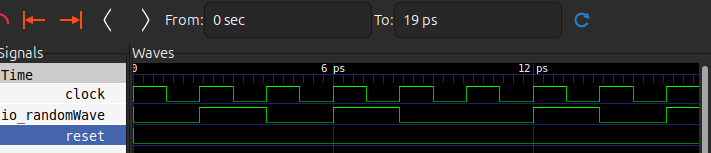
\includegraphics[width=\textwidth]{Images/verilator_waveformgenerator_screenshot.png} 
    \caption{Waveforms for generated SystemVerilog Verilator simulation}
    \label{fig:verilator_wave}
\end{figure}

\includechiselcode[caption={Waveform Generator Code with Emit SystemVerilog (Chisel)},     label={lst:chisel_waveformgenerator_emit_sv}, firstline=26, firstnumber=26, lastline=29]{\chiselSourceDir/waveFormGenerator.scala}

Chisel has the capability to emit SystemVerilog, Verilog, Waveforms (vcd), and circuit diagrams (svg). Section \ref{sub:verilator_test_driver} shows the process for generating the waveform shown in Figure \ref{fig:verilator_wave}. It uses Verilator rather than internal Chisel output.
}%end chisel

\ifthenelse{\boolean{verilogversion}}{
%*********************************************************
\subsubsection{SystemVerilog Implementation of Waveforms}
%*********************************************************    
\includeverilogcode[caption={Waveform Generator Code (Hand Written Verilog)},     label={lst:verilog_waveformgenerator}, firstline=8, firstnumber=8, lastline=999]{\verilogSourceDir/waveFormGenerator.sv}

Listing \ref{lst:verilog_waveformgenerator} shows the hand written SystemVerilog module, \texttt{waveFormGenerator}. It generates two output waveforms: a \texttt{randomWave} signal and a \texttt{clock} signal. The \texttt{randomWave} signal transitions between predefined states based on explicit delays specified using the \texttt{\#} operator. It begins at \texttt{0}, transitions to \texttt{1} after 2 time units, back to \texttt{0} after 6 more time units, to \texttt{1} after 4 additional time units, and finally to \texttt{0} after 8 time units. The simulation halts 5 time units later using the \texttt{\$stop} command. The \texttt{clock} signal is a periodic waveform toggling its state every 2 time units, implemented with a \texttt{forever} loop.

\placedrawing[H]{figures/01_02_waveSim.lp}{Waveforms generated by Vivado for hand written SystemVerilog simulation}{fig:vivado_wave}

Figure \ref{fig:vivado_wave} shows the results of simulating the {\tt waveFormGenerator.sv} module using Vivado.

}%end verilog

\ifthenelse{\boolean{verilogversion} \and \boolean{chiselversion}}{   
%*********************************************************************************
\subsubsection{Comparison of Chisel and SystemVerilog Implementation of Waveforms}
%**********************************************************************************
In the Chisel implementation of the \texttt{waveFormGenerator}, the functionality is expressed using high-level abstractions. The \texttt{randomWave} is generated as a cyclic sequence of Boolean values, and its transitions are determined by a counter that increments on every clock cycle. Unlike the Verilog version, the Chisel implementation does not explicitly emulate timing delays but instead assumes uniform timing for each state in the sequence. 

While both implementations generate a \texttt{randomWave} and a clock-like signal, they differ in their timing behavior and functionality. The Verilog version explicitly specifies time delays for signal transitions and provides a clear stop condition using \texttt{\$stop}. The Chisel version is higher-level, more abstract, and assumes regular timing intervals without emulating the exact delays. This makes the Chisel version more suitable for hardware synthesis, where timing is managed by the clock, while the Verilog version offers precise control for simulation purposes.
}%end both true

%%%%%%%%%%%%%%%%%%%%%%%%%%%%%%%%%%%%%%%%%%%
\section{One-Input Combinational Circuits}
%%%%%%%%%%%%%%%%%%%%%%%%%%%%%%%%%%%%%%%%%%%
Combinational circuits are a fundamental type of digital circuit where the outputs are determined solely by the current inputs, without any memory or feedback elements. They perform logical and arithmetic operations based on Boolean algebra. Examples of combinational circuits include logic gates (AND, OR, NOT), arithmetic circuits (adders, subtractors), and data routing components (multiplexers, encoders). These circuits are deterministic, meaning their outputs are uniquely determined by the given inputs \cite{mano2017}.

%******************************
\subsection{Formal Description}
%******************************
A one-input combinational circuit is a digital logic circuit where the output depends solely on the value of a single binary input \( A \). Such circuits are governed by a Boolean function \( f(A) \), where \( f: \{0, 1\} \to \{0, 1\} \). The output is computed instantaneously based on the input value, with no memory or feedback elements involved. The behavior of the circuit can be described by a truth table, which enumerates the two possible input values (\( A = 0 \) and \( A = 1 \)) and their corresponding outputs (\( f(0) \) and \( f(1) \)). 

\begin{table}[H]
  \begin{center}
    \caption{One-input circuits.}
    \label{tab:one_input_circuits}
    \begin{tabular}{|c||c|c|c|}
      \hline
      A&  &  NOT&  BUFFER      \\ \hline \hline
      0&  &   1&       0    \\ \hline
      1&  &   0&       1    \\ \hline
    \end{tabular}
  \end{center}
\end{table}

\placedrawing[H]{figures/02_01_not.lp}{Graphic representation of the NOT and BUFFER circuits.}{fig:one_input_ckt}

Table \ref{tab:one_input_circuits} shows the truth table for a NOT gate, which inverts the input (\( f(A) = \neg A \)), and BUFFER (constant) circuit, which outputs a fixed value regardless of the input (\( f(A) = 0 \) or \( f(A) = 1 \)). Figure \ref{fig:one_input_ckt} shows the logic circuit symbol of the NOT and BUFFER combinational circuits. This is also called a gate symbol.

%***************************************************
\subsection{Physical Implementation of NOT Circuit}
%***************************************************
The physical implementation of a NOT circuit, or inverter, bridges the abstract concept of Boolean algebra with real-world digital hardware. A NOT gate takes a single input and produces an output that is its logical complement. In practice, this is typically achieved using transistor-based designs, such as CMOS (Complementary Metal-Oxide-Semiconductor) technology. 

The delay inherent in a NOT circuit, commonly referred to as the \emph{gate delay}, arises from the physical properties of the transistors and the interconnects. When the input changes state, the transistors must charge or discharge the capacitive load at the output. This charging and discharging process is influenced by factors such as the capacitance of the output node, the resistance of the transistors, and the speed of the power supply. As a result, the propagation delay, defined as the time taken for the output to reach a certain percentage of its final value after a change in input, becomes an important metric in digital circuit performance. 

Understanding where gate delays originate is important for designing circuits that meet timing requirements in high-speed applications. The interested reader can consult Appendix \ref{app:physical_implementations} for more information.

%%%%%%%%%%%%%%%%%%%%%%%%%%%
\section{Two-input gates}
%%%%%%%%%%%%%%%%%%%%%%%%%%%
Two-input gates depend on two binary inputs. Common two-input gates include AND, OR, XOR, NAND, and NOR. 

%*******************************
\subsection{Formal Description}
%******************************
Two-input gates are fundamental components in digital logic that perform Boolean operations on two binary variables, \( A \) and \( B \), to produce a single output \( f(A, B) \). Mathematically, these gates implement functions \( f: \{0, 1\} \times \{0, 1\} \to \{0, 1\} \), where the domain consists of all possible ordered pairs of binary inputs, and the range is restricted to binary outputs. 

Each type of two-input gate corresponds to a specific Boolean operation, such as AND (\( f(A, B) = A \land B \)). The behavior of these gates can be fully specified using truth tables, which enumerate all possible input combinations and their corresponding outputs.

\begin{table}[H]
  \begin{center}
    \caption{Two-input Combinational Gates Truth Table.}
    \label{tab:two_input_gates}
    \begin{tabular}{|c|c||c|c|c|c|c|c|}
      \hline
      $A$& $B$&   OR&        NOR&              AND&     NAND&              XOR&         XNOR \\ 
       &  &  $A\lor B$ & $\neg (A \lor B)$& $A\land B$& $\neg (A \land B)$&  $A\oplus B$&   $\neg (A \oplus B)$                              \\ \hline \hline
      0& 0&  0&         1&                 0&       1&                  0&           1\\ \hline
      0& 1&  1&         0&                 0&       1&                  1&           0\\ \hline
      1& 0&  1&         0&                 0&       1&                  1&           0\\ \hline
      1& 1&  1&         0&                 1&       0&                  0&           1\\ \hline
    \end{tabular}
  \end{center}
\end{table}

Table \ref{tab:two_input_gates} shows the truth table for combinational 2-input gates and Table \ref{tab:logic_gates_summary} shows the summary of their interpretations.

\begin{description}
\item[AND]: \( A \cdot B = AB \), where \( AB = 1 \) only if both \( A \) and \( B \) are 1, otherwise \( AB = 0 \). \\
    Numerical interpretation: Arithmetic product. \\
    Symbolic interpretation:  Gate, because \( A = 1 \) opens the way for \( B \). \\
    Alternative names: Conjunction, multiply gate, all-or-nothing gate \cite{boole1854book, rosen2018}.

\item[NAND]: \( \neg (A \cdot B) \), where the output is \( 0 \) only if both \( A \) and \( B \) are 1; otherwise, the output is \( 1 \). \\
    Symbolic interpretation: Universal gate. \\
    Alternative names: Sheffer stroke, negated AND gate \citep{sheffer1913, rosen2018}.

\item[OR]: \( A + B \), where \( A + B = 1 \) if at least one of \( A \) or \( B \) is \( 1 \); otherwise, \( A + B = 0 \). \\
    Symbolic interpretation: Inclusive OR. \\
    Alternative names: Disjunction, any-or-all gate \cite{rosen2018}.

\item[NOR]: \( \neg (A + B) \), where the output is \( 0 \) if at least one of \( A \) or \( B \) is \( 1 \); otherwise, the output is \( 1 \). \\
    Symbolic interpretation: Universal gate. \\
    Alternative names: Peirce arrow, negated OR gate \cite{peirce1885, rosen2018}.

\item[XOR]: Exclusive OR, because it excludes the case \( A = B = 1 \) in determining \( 1 \) on the output. \\
    \( A \oplus B = 1 \) when only one of the inputs \( A \) or \( B \) is \( 1 \). \\
    Logic interpretation: Conditioned inverter, i.e., \( \text{if } A = 0 \text{ then } A \oplus B = B, \text{ else } A \oplus B = B' \). \\
    Numerical interpretation: Modulo-2 sum. \\
    Symbolic interpretation: Anticoincidence. \\
    Alternative names: Either-or gate, modulo-2 adder \cite{shannon48, rosen2018}.

\item[XNOR]: \( \neg (A \oplus B) \). \\
    Symbolic interpretation: Coincidence. \\
    Alternative names: Equality gate, NOT XOR \cite{mano2017, rosen2018}.
\end{description}

\begin{table}[htbp]
\centering
\renewcommand{\arraystretch}{1.5} % Adjust row height
\setlength{\tabcolsep}{5pt} % Adjust column spacing
\begin{tabular}{|>{\centering\arraybackslash}p{2cm}|>{\centering\arraybackslash}p{3cm}|>{\centering\arraybackslash}p{2cm}|>{\centering\arraybackslash}p{5cm}|}
\hline
\textbf{Logic Gate} & \textbf{Numerical} & \textbf{Symbolic} & \textbf{Alternative Names} \\ \hline

OR  & Logical addition (no carry) \( A + B \) & \( A \lor B \) & Disjunction, Any-or-All Gate, Inclusive OR \\ \hline

NOR  & Complement of OR: \( 1 - (A + B) \) & \( \neg (A \lor B) \) & Peirce Arrow, Negated OR Gate, Universal Gate \\ \hline

AND & Logical multiplication \( A \cdot B \) & \( A \land B \) & Conjunction, Multiply Gate, All-or-Nothing Gate \\ \hline

NAND  & Complement of AND: \( 1 - (A \cdot B) \) & \( \neg (A \land B) \) & Sheffer Stroke, Negated AND Gate, Universal Gate \\ \hline

XOR  & Modulo-2 addition \( A \oplus B \) & \( A \oplus B \) & Exclusive OR, Modulo-2 Adder, Anticoincidence \\ \hline

XNOR  & Complement of XOR: \( 1 - (A \oplus B) \) & \( \neg (A \oplus B) \) & Exclusive NOR, Equality Gate, Coincidence \\ \hline

\end{tabular}
\caption{Summary of Logical Gates and their Interpretations}
\label{tab:logic_gates_summary}
\end{table}

Many of the historical names in \ref{tab:logic_gates_summary} stem from different disciplines. Terms like conjunction, disjunction, and negation originate from symbolic logic. Coincidence and anticoincidence were used in early telecommunications signal processing contexts. Practical descriptions like multiply gate and modulo-2 adder reflect the role of these gates in arithmetic and data processing. Modern digital logic has largely standardized the terms AND, OR, XOR, etc., as defined by IEEE and other standard bodies \cite{ieee_std_91}.

\placedrawing[H]{figures/02_07_two_input_gates.lp}{Graphical representation of the most used two-input gates.}{fig:graphical_gates}
Figure \ref{fig:graphical_gates} shows the graphical representations of logic gates. These originated from the need to visually depict logical operations in a way that facilitated the design and analysis of digital systems. These representations were inspired by symbolic logic and Boolean algebra, where logic functions were expressed using abstract symbols. Early pioneers, such as Claude Shannon, formalized the connection between Boolean algebra and electronic circuits, enabling the translation of logical expressions into circuit designs \cite{shannon48}. Over time, distinct shapes were assigned to each gate for clarity—such as the triangular symbol for NOT gates and the curved line for OR gates. Standardization efforts by organizations like the IEEE and IEC later codified these symbols, ensuring universal recognition and consistency in circuit diagrams \cite{ieee_std_91}. 


\placedrawing[H]{figures/02_08_non_inverting_gate_waveforms.lp}{Wave forms for the non-inverting gates.}{fig:waveforms}
Waveforms are tools used in digital logic for visualizing and analyzing the behavior of signals over time. They represent the changes in voltage levels for inputs, outputs, and intermediate nodes in a circuit, making it easier to understand timing relationships, transitions, and delays. The use of waveforms emerged alongside the development of oscilloscopes and other signal measurement tools in the early 20th century, as engineers needed a method to observe electrical signals in real-time. With the advent of digital systems, waveforms became a standard way to represent binary signals, where high and low voltage levels correspond to logical 1s and 0s, respectively. Waveforms allow engineers to verify the correct operation of logic circuits and diagnose timing-related issues such as glitches, race conditions, and setup/hold violations \cite{horowitz1993, ieee_waveform}. Their graphical nature complements schematic diagrams by providing temporal information that is not inherently visible in static circuit representations.


Figure \ref{fig:waveforms} shows the behavior of AND, OR and XOR gates. They are driven by the signals $A$ and $B$ represented in the first two wave forms. Besides the logic response to the inputs, timing characteristics are also shown. 
\begin{itemize}
    \item $t_+$: the positive transition time (the duration of the positive edge)
    \item $t_-$: the negative transition time (the duration of the negative edge)
    \item $t_{pLH}$: the propagation time  of the signal through the gate for the transition from Low to High
    \item $t_{pHL}$: the propagation time  of the signal through the gate for the transition from High to Low
\end{itemize}

We leave the treatment of timing to a course on digital logic design. It is a critical component in building working systems but is abstracted away in this book.

%%%%%%%%%%%%%%%%%%%%%%%%%%%
\section{Many-Input Gates}
%%%%%%%%%%%%%%%%%%%%%%%%%%%
Many-input gates are an essential extension of basic logic gates, allowing the combination of more than two inputs into a single logical operation. These gates operate based on the principles of Boolean algebra and are widely used in digital systems to manage complex logical expressions. For instance, an \( n \)-input AND gate outputs a logical \( 1 \) only when all \( n \) inputs are \( 1 \), while an \( n \)-input OR gate outputs \( 1 \) when at least one of the inputs is \( 1 \). As the number of inputs increases, the complexity of the gate's behavior grows exponentially, governed by the number of possible input configurations.

Mathematically, the total number of distinct \( n \)-input gates is \( N^{2^n} \), where \( N \) represents the number of possible output values (typically \( N = 2 \) for binary logic), and \( 2^n \) is the total number of unique input configurations for \( n \) inputs. This exponential growth means that even for relatively small \( n \), the number of possible logic gates becomes vast and impractical to enumerate. For example, with \( n = 3 \), there are \( 2^{2^3} = 256 \) possible gates. For \( n > 2 \), Boolean algebra rules are necessary for simplifying and managing these functions, enabling the design of practical circuits without explicitly listing all possible gates.

In modern digital design, many-input gates are often implemented using a combination of smaller gates, as direct implementation can become physically and computationally impractical for large \( n \). For example, a 16-input AND gate might be constructed hierarchically by combining multiple 2-input AND gates. This modular approach leverages the fundamental properties of Boolean algebra to efficiently implement complex logical functions in hardware. 


Let's consider some significant examples:

\begin{itemize}
    \item (A')' = A
    \item AB + AB' = A(B + B') = A $\cdot$ 1 = A\\
    When B=1 the expression takes the value A, and when B=0 the expression still takes the value A, we conclude that the value of B does not matter and the expression takes the value A.
    \item A + A'B = A + B\\
    This can be proved by the truth table in Table \ref{tab:truth_table_proof}.
    \begin{table}[H]
  \begin{center}
    \caption{Truth table proof of A + A'B = A + B.}
    \label{tab:truth_table_proof}
    \begin{tabular}{|c|c||c|c|c||c|}
      \hline
      A& B&  A'& A'B& A+A'B& A+B   \\ \hline \hline
      0& 0&   1&   0&     0&   0   \\ \hline
      0& 1&   1&   1&     1&   1   \\ \hline
      1& 0&   0&   0&     1&   1   \\ \hline
      1& 1&   0&   0&     1&   1   \\ \hline
    \end{tabular}
  \end{center}
\end{table}
    \item A $\oplus$ B = (A' $\oplus$ B)' = (A $\oplus$ B')' = A' $\oplus$ B'
    \item A + B = (A'B')' \\
    From de Morgan's rule, A or B is 1 is equivalent to the fact that it is not true that A is 0 and B is 0.
    \item AB = (A' + B')'\\
    From de Morgan rule, A and B are 1 is equivalent to the fact that it is not true that A is 0 or B is 0.
\end{itemize}

%*********************************
\subsection{Seven-Segment Display}
%*********************************
A 7-segment display is a common example of a combinational circuit that illustrates the concept of many-input logic gates. It consists of seven individual segments, labeled a through g, which can be illuminated to form numerical digits (0–9). The control logic for a 7-segment display is designed as a combinational circuit that takes a binary-coded decimal (BCD) input, typically 4 bits, and determines which segments should be activated to display the corresponding digit. Each segment is controlled by a Boolean expression derived from the binary input, effectively making the display a complex many-input gate. The circuit highlights how combinational logic can efficiently decode binary inputs into human-readable visual representations.

% FIXME: Get a 7-segment only drawing
\placedrawing[H]{figures/01_03_7seg_and_adder.lp}{The version of digital circuits. {\bf a.} Logic circuit: trans-coder for seven-segment display. {\bf b.} Numeric circuit: four-bit numbers adder.}{fig:7_segment_display}

Figure \ref{fig:7_segment_display} shows the transcoder for a 7-segment display. It receives four-bit coded decimal numbers, from 0 to 9, and convert them in 7-bit codes, a to g, indicating the segments to be activated, according to Table \ref{tab:sevenSeg}.

The logic expression for the output {\tt a} is:
\begin{center}
$a =   B'_3 \cdot B'_2 \cdot B'_1\cdot B'_0  + B'_3 \cdot B'_2 \cdot B_1\cdot B'_0  +
        B'_3 \cdot B'_2 \cdot B_1\cdot B_0  + B'_3 \cdot B_2 \cdot B'_1\cdot B_0  + $ \\
        $B'_3 \cdot B_2 \cdot B_1\cdot B'_0  + B'_3 \cdot B_2 \cdot B_1\cdot B_0  +
        B_3 \cdot B'_2 \cdot B'_1\cdot B'_0  + B_3 \cdot B'_2 \cdot B'_1\cdot B_0  $
\end{center}
or a simpler version by negatin the negated function:
$$a =  (a')' =  (B'_3 \cdot B'_2 \cdot B'_1\cdot B_0  + B'_3 \cdot B_2 \cdot B'_1\cdot B'_0)' = (B'_3 \cdot B'_1 \cdot (B_2 \oplus B_0))' = B_3 + B_1 + (B_2 \oplus B_0)'$$


\begin{table}[H]
  \begin{center}
    \caption{Seven-segment display truth table.}
    \label{tab:sevenSeg}
    \begin{tabular}{|c||c|c|c|c||c|c|c|c|c|c|c|}
      \hline
     & $B_3$ & $B_2$ & $B_1$ & $B_0$ & a & b & c & d & e & f & g \\ \hline \hline
     0& 0 & 0 & 0 & 0 & 1 & 1 & 1 & 1 & 1 & 1 &   \\ \hline % 0
     1& 0 & 0 & 0 & 1 &    & 1 & 1 &    &    &    &   \\ \hline % 1
     2& 0 & 0 & 1 & 0 & 1 & 1 &    & 1 & 1 &    & 1 \\ \hline % 2
     3& 0 & 0 & 1 & 1 & 1 & 1 & 1 & 1 &    &    & 1 \\ \hline % 3
     4& 0 & 1 & 0 & 0 &    & 1 & 1 &    &    & 1 & 1 \\ \hline % 4
     5& 0 & 1 & 0 & 1 & 1 &    & 1 & 1 &    & 1 & 1 \\ \hline % 5
     6& 0 & 1 & 1 & 0 & 1 &    & 1 & 1 & 1 & 1 & 1 \\ \hline % 6
     7& 0 & 1 & 1 & 1 & 1 & 1 & 1 &    &    &    &   \\ \hline % 7
     8& 1 & 0 & 0 & 0 & 1 & 1 & 1 & 1 & 1 & 1 & 1 \\ \hline % 8
     9& 1 & 0 & 0 & 1 & 1 & 1 & 1 & 1 &    & 1 & 1 \\ \hline % 9
    \end{tabular}
  \end{center}
\end{table}

%#######################
% 7 Segment Display Code
%#######################
\ifthenelse{\boolean{chiselversion}}{
%*************************************************
\subsubsection{Seven Segment Display (Chisel)}
%*************************************************
\includechiselcode[caption={Seven Segment Display (Chisel)},     label={lst:chisel_sevensegmentdisplay}, firstline=9, firstnumber=9, lastline=28]{\chiselSourceDir/SevenSegmentDisplay.scala}

Listing \ref{lst:chisel_sevensegmentdisplay} shows the \texttt{SevenSegmentDisplay} class is a Chisel module that decodes a 4-bit binary input (\texttt{binIn}) into a 7-bit output (\texttt{segOut}) representing the activation of segments on a seven-segment display. The input, \texttt{binIn}, can take values from 0 to 9, and the module determines which segments (labeled \texttt{a} through \texttt{g}) should be illuminated to form the corresponding numeric digit on the display.

The decoding logic is implemented using a series of \texttt{when} and \texttt{elsewhen} constructs. Each condition compares \texttt{binIn} with a specific value and assigns a 7-bit binary pattern to \texttt{segOut}. Each bit in the pattern corresponds to one of the seven segments, where a \texttt{1} turns the segment on, and a \texttt{0} turns it off. For example, when \texttt{binIn} is \texttt{0}, the output is \texttt{1111110}, which activates all segments except \texttt{g} to display the digit \texttt{0}. Similarly, for \texttt{binIn = 8}, all segments are activated (\texttt{1111111}). A default value of \texttt{0000000} is set for \texttt{segOut} to ensure all segments are off in case of invalid input.

In Chisel 6.6, the use of the \texttt{switch} function is discouraged because it often leads to less modular and harder-to-read code, especially in large designs. The \texttt{switch} function can introduce an implicit and tightly coupled relationship between the control signal and the cases, reducing flexibility and increasing the risk of errors during refactoring. Instead, Chisel promotes the use of more functional constructs like pattern matching or chained \texttt{when} statements which makes the design less prone to subtle bugs.

}%End Chisel

\ifthenelse{\boolean{verilogversion}}{
%*********************************************************
\subsubsection{Seven Segment Display (SystemVerilog)}
%*********************************************************    
\includeverilogcode[caption={Seven Segment Display (Hand Written Verilog)},     label={lst:verilog_sevensegmentdisplay}, firstline=7, firstnumber=7, lastline=999]{\verilogSourceDir/SevenSegmentDisplay.sv}

Listing \ref{lst:verilog_sevensegmentdisplay} shows SystemVerilog code that implements a seven-segment display decoder. The module, named \texttt{sevenSegmDys}, has a 4-bit binary input, \texttt{number}, and a 7-bit output, \texttt{seg}, which controls the state of the seven segments (labeled a through g) of the display. 

The \texttt{always\_comb} block defines a combinational block that describes the behavior of the output of the circuit as a combination based on the value of the input variables. The blocking assignment, {\tt =}, is used to assure the combinational behavior.

The \texttt{case} statement maps each possible input value (0 through 9) to a corresponding 7-bit output pattern that activates the appropriate segments to display the digit. For example, the binary input \texttt{4'b0000} (decimal 0) results in the output \texttt{7'b1111110}, which lights up all segments except \texttt{g}, forming the number 0 on the display.

The module includes a \texttt{default} case that sets all segments to off (\texttt{7'b0000000}) for invalid inputs outside the range 0–9. By mapping each input to a fixed segment configuration, this module can be integrated into larger digital systems that require visual representation of numeric values, such as timers, calculators, or embedded control systems.


}%End SystemVerilog

\ifthenelse{\boolean{verilogversion} \and \boolean{chiselversion}}{   
%*********************************************************************************
\subsubsection{Seven Segment Display Language Comparison}
%**********************************************************************************
The Chisel and SystemVerilog implementations both utilize conditional logic. Chisel uses \texttt{when} statements, while SystemVerilog uses a \texttt{case} statement within an \texttt{always\_comb} block. The primary difference are due to the design of the two languages. Chisel, being embedded in Scala, provides a high-level, functional programming approach, emphasizing abstraction and type safety. SystemVerilog is a traditional hardware description language explicitly designed for synthesizable digital circuits. Chisel initializes the \texttt{segOut} output to a default value, simplifying handling unspecified input cases, while SystemVerilog uses the \texttt{default} case explicitly within its \texttt{case} statement. 

Moreover, SystemVerilog's \texttt{always\_comb} guarantees that the logic produced is purely combinational, making the designer's intent explicit. In contrast, Chisel does not inherently enforce combinational logic; it depends on how constructs like \texttt{when} are used. For instance, \texttt{when} can describe sequential behavior if used with registers, but in the given example, the direct use of \texttt{:=} ensures combinational behavior.

}
%################################
% End Seven Segment Display Code
%################################

%%%%%%%%%%%%%%%%%%%%%%%%%%%%%%%%%%%%%%%%%%%%%%%%%%%%%%%%%%%%%%%%%%%%%%%%%%%%%%%%%%%%%%%%%%%%%%%%%%%
\section{Generic combinational circuits}
%%%%%%%%%%%%%%%%%%%%%%%%%%%%%%%%%%%%%%%%%%%%%%%%%%%%%%%%%%%%%%%%%%%%%%%%%%%%%%%%%%%%%%%%%%%%%%%%%%%
%*******************
\subsection{Decoder}
%********************
Figure \ref{fig:decoder} how to design a 3-bit decoder. Decoding means to identify with a one bit signal each binary code applied to the input of the circuit. Therefore, a $n$-bit input code applied on the input of a decoder implies a number of $2^n$ outputs. Only one output is active at a time, corresponding to the input code. Thus, for the decoder represented in Figure \ref{fig:decoderr}, if $\{x_{n-1}, \ldots, x_0\} = 00 \ldots 0101$, then $y_5=1$ and all the other outputs are 0.

\placedrawing[H]{figures/02_09_decoder.lp}{Decoder with $n$-bit input (DCDn).}{fig:decoder}

%#######################
% Decoder Code
%#######################
\ifthenelse{\boolean{chiselversion}}{
%*************************************************
\subsubsection{Decoder (Chisel)}
%*************************************************
\includechiselcode[caption={Parameterized Decoder (Chisel)}, label={lst:chisel_decoder}, firstline=9, firstnumber=9, lastline=999]{\chiselSourceDir/Decoder.scala}


}%End Chisel

\ifthenelse{\boolean{verilogversion}}{
%*********************************************************
\subsubsection{Decoder (SystemVerilog)}
%*********************************************************    
\includeverilogcode[caption={Parameterized Decoder (Hand Written SystemVerilog)},     label={lst:verilog_decoder}, firstline=8, firstnumber=8, lastline=999]{\verilogSourceDir/dcdParmeterized.sv}


\includeverilogcode[caption={Behavioral Decoder (Hand Written SystemVerilog)},     label={lst:verilog_decoder}, firstline=8, firstnumber=8, lastline=999]{\verilogSourceDir/dcd.sv}

}% End Verilog




The System Verilog code for the decoder circuit follows. The description is behavioral.

\begin{verisum}{\em :

\hspace{-0.8cm} \rule[5mm]{16cm}{0.25mm} \vspace{-0.7cm}

\begin{description}
    \item[$<<$]: shift left logical, i.e., multiplication with 2 to the power of the number of binary shifts
\end{description}
\rule[5mm]{16cm}{0.25mm} }
\end{verisum}





In Figure \ref{fig8}a, is represented the smallest decoder, the elementary DCD, eDCD. Using two eDCD and 4 ANDs, a two-input decoder, DCD2, is designed (see Figure \ref{fig8}b). The rule to increase the number of inputs becomes evident with the third example: DCD3 (see Figure \ref{fig8}c).


\placedrawing[H]{figures/02_10_recursive_decoder.lp}{Recursively defined 3-input decoder (DCD). {\bf a.} Elementary decoder (eDCD). {\bf b.} Two-input decoder (DCD2). {\bf c.} Three-input DCD (DCD3).}{fig8}


\subsection{Multiplexor}

\subsection{Elementary multiplexor}

Any combinational circuit can be expressed using NAND function. But a more interesting "fundamental brick" could be a circuit corresponding to the ubiquitous {\bf {\em if-then-ellse}} statement. It is the elementary multiplexor (eMUX) represented in Figure \ref{fig9},
where:

\placedrawing[H]{figures/02_11_mux.lp}{Elementary multiplexor (eMUX). {\bf a.} The circuit structure: an eDCD serially connected with an AND-OR circuit. {\bf b.} The logic symbol.}{fig9}

\begin{center} O = {\bf if} (S) {\bf then} I1 {\bf else} I0 \end{center}

\subsection{Many-input multiplexor}

The multiplexor grabs bits from $m=2^n$ inputs selected by a $n$-bit code.

\placedrawing[H]{figures/02_12_mux_generalized.lp}{The general definition of the multiplexor circuit (MUXn). {\bf a.} The structure of MUXn: a DCDn serially connected with a $m=2^n$ ANDs on the first level of an AND-OR structure. {\bf b.} The logic symbol for MUXn.}{fig12}


\begin{verisum}{\em :

\hspace{-0.8cm} \rule[5mm]{16cm}{0.25mm} \vspace{-0.7cm}

\begin{description}
    \item[{\tt a[b]}]: selects the bit indicated by {\tt b} from the binary word {\tt a}
\end{description}
\rule[5mm]{16cm}{0.25mm} }
\end{verisum}

{\small
\begin{shaded*}
\begin{lstlisting}[language=Verilog, caption= , morekeywords={always_ff, always_comb, logic, loop, repeat, doInParallel, for}]
/*************************************************************************
File name:      mux.sv
Circuit name:   4-input multiplexor
Description:
*************************************************************************/
module mux( output  logic           muxOut  ,
            input   logic [15:0]    muxIn   ,
            input   logic [3:0]     muxSel  );

     assign muxOut = muxIn[muxSel] ;
endmodule
\end{lstlisting}
\end{shaded*}
}


\subsection{Demultiplexor}

The demultiplexer transfers the input signal X to one of the $m=2^n$ outputs, $y_0, y_1, \ldots, y_{m-1}$, indicated by the $n$-bit selection input, $x_0, x_1, \ldots, x_{n-1}$. In Figure \ref{fig13} a demultiplexer is built using a decoder which open only one of the $m$ AND gate sending the $X$ input to the selected output.

\placedrawing[H]{figures/02_13_demux.lp}{Demultiplexor as a DCD whose outputs are ANDed with the one bit signal to be distributed according to the $n$-bit input code. }{fig13}


For example: if $$\{x_{n-1} x_{n-2}, \ldots, x_1, x_0\} = 00 \ldots 011$$ then
$$\{y_{m-1} y_{m-2} \ldots y_0 y_1\} = 00 \ldots 0X000$$

The code describing behaviorally the circuit follows:

{\small
\begin{shaded*}
\begin{lstlisting}[language=Verilog, caption= , morekeywords={always_ff, always_comb, logic, loop, repeat, doInParallel, for}]
/*************************************************************************
File name:      dMux.sv
Circuit name:   4-input demultiplexor
Description:    Demultiplexor is an enabled decoder
*************************************************************************/
module dMux(output  logic [15:0]    dMuxOut     ,
            input   logic [3:0]     dMuxIn      ,
            input   logic           dMuxEnable  );

     assign dMuxOut = dMuxEnable << dMuxIn ;
endmodule
\end{lstlisting}
\end{shaded*}
}
Now, instead of left-shifting the number 1 as in the decoder, the one-bit value $X$ is left-positioned.


\section{Function oriented combinational circuits}

\subsection{Half Adder}

As we have seen, the XOR circuit calculates the sum modulo 2 but does not differentiate between 0+0 and 1+1. This differentiation involves the calculation of the arithmetical overshoot, which we denote by carry (to the next binary order). Carry signal is activated when both inputs are 1. Therefore, besides the XOR gate we must add an AND gate as in Figure \ref{fig3}. We call the resulting circuit half adder because it does not take into account the carry signal provided by the previous binary order.

\placedrawing[H]{figures/02_14_half_adder.lp}{Half adder (HA).The XOR circuit compute the {\em modulo-2} sum while the AND gate compute the carry value.}{fig3}


\subsection{Increment}

Incrementing means adding 1 to a number. The schematic for a 4-bit increment circuit, INC4, is represented in Figure \ref{fig4}, where if {\tt inc = 1} the output $out_0 <= in'_0$  and {\tt cr} of $HA_0$ if it is activated command the increment for $HA_1$, and so on.

\placedrawing[H]{figures/02_15_increment.lp}{Increment circuit for 4-bit numbers (INC4) implemented by serially connected $4$ HAs.}{fig4}

If each 2-input AND from $HA_i$ has, for example,  a propagation time, $t_{pAND2} = 1ns = 10^{-9}sec$, and the 2-input XOR has the propagation time, $t_{pXOR2} = 1.5ns$, then the total execution time for the INC4 circuit is:
$$t_{pINC4} = 3 \times t_{pAND2} + t_{pXOR2} = 4.5ns$$
Thus, when the good news that the size of the $n$-bit number increment circuit, $S_{INCn}$, is proportional with the input size, the bad news is that the execution time, i.e., depth, $D_{INCn}$, is in same magnitude order:
$$S_{INCn} \in O(n)$$
$$D_{INCn} \in O(n)$$
(The depth of the circuit can be reduced by increasing the size (but in the limits of the same magnitude order) using a prefix network.)

\subsection{Adder/subtractor}

Full adder (FA) adds two one-bit numbers with the carry provided from the previous binary position and generate the sum and the carry value for the next binary position. In Figure \ref{fig5}a, a FA is composed from two HAs and an OR circuit used to grab the carry generated by the first HA or by the second HA. The first FA adds the two input bits, A and B, while the second FA adds the value of the carry, C, generated by the previous binary order.

\placedrawing[H]{figures/02_16_adder_full.lp}{Adder. {\bf a.} Full Adder (FA). {\bf b.} 4-bit adder (ADD4).}{fig5}

\placedrawing[H]{figures/02_17_adder_subtractor.lp}{Adder/Substractor}{fig6}


The main problem to be solved, but not in this lecture, is the execution time, i.e., the maximum time interval from the moment when an input changes until the moment when all the outputs of the circuit reach the correct final value. This time interval is due to propagation through logic gates on the longest path. In our case, the longest path is the one from input C to output $C_{out}$. On this path there are 8 logic gates, one AND and one OR for each binary order. In the general case, the time is proportional to $n$ (it is in $O(n)$).





Subtract operation is performed by adding the 2s complement:

\begin{verbatim}
        +5 = 0_0101
        -5 = 1_1010 + 1 = 1_1011
        +5 = 0_0100 + 1 = 0_0101

        -5 + 2 = 1_1011 +
                 0_0010 =
                 1_1101 = -3, because 0_0010 + 1 = 0_0011 = 3
\end{verbatim}

Therefore, each $B_i$ is complemented and the increment with 1 is generated by inverting the carry input. All the inversions are performed under de command {\tt sub} applied to $5$ XORs.


\subsection{{\bf {\em Arithmetic \& Logic Unit}}}\label{alu1}

An Arithmetic \& Logic Unit (ALU) has two kinds of connections: data inputs and outputs, for the $n$-bit operands, and command inputs for the operations applied to operands (see Fig \ref{fig37}). In Figure \ref{fig15}, is represented the generic form of an ALU with 8 functions each performed in a distinct module, {\tt func0, ..., func7}, whose outputs are selected by a multiplexor as the result by the {\tt func} code. The two operands, {\tt leftOp[n-1:0], rightOp[n-1:0]}, are applied to all the 8 modules.

\placedrawing[H]{figures/02_18_alu.lp}{ALU.}{fig37}


\placedrawing[H]{figures/02_19_8function_alu.lp}{The generic form of a 8-function Arithmetic \& Logic Unit for $n$-bit words (ALUn).}{fig15}

{\small
\begin{shaded*}
\begin{lstlisting}[language=Verilog, caption= , morekeywords={always_ff, always_comb, logic, loop, repeat, doInParallel, for}]
/*************************************************************************
File name:      alu.sv
Circuit name:   arithmetic and logic unit
Description:    the circuit selects, using the selection code 'func', one
                of the 8 functions
*************************************************************************/
module ALU(input    logic         crIn          ,
            input   logic [2:0]   func          ,
            input   logic [31:0]  left, right   ,
            output  logic         crOut         ,
            output  logic [31:0]  out           );

  always_comb case(func)
                3'b000: {crOut, out} = left + right + crIn;     //add
                3'b001: {crOut, out} = left - right - crIn;     //sub
                3'b010: {crOut, out} = {1'b0, left & right};    //and
                3'b011: {crOut, out} = {1'b0, left | right};    //or
                3'b100: {crOut, out} = {1'b0, left ^ right};    //xor
                3'b101: {crOut, out} = {1'b0, ~left};           //not
                3'b110: {crOut, out} = {1'b0, left};            //left
                3'b111: {crOut, out} = {1'b0, left >> 1};       //shr
            endcase
endmodule
\end{lstlisting}
\end{shaded*}
}

\begin{verisum}{\em :

\hspace{-0.8cm} \rule[5mm]{16cm}{0.25mm} \vspace{-0.7cm}

\begin{description}
    \item[\{a,b\}]: concatenates the binary word  {\tt b} to the binary word {\tt a}
    \item[{\bf -}]:  is the operator {\tt minus}
    \item[\&]: is the operator {\tt bitwise AND}
    \item[${\bf \vert}$]: is the operator {\tt bitwise OR}
    \item[${\bf \hat{}}$]: is the operator {\tt bitwise XOR}
    \item[${\bf >>}$]: is the operator {\tt shift right logical}
\end{description}
\rule[5mm]{16cm}{0.25mm} }
\end{verisum}

Actual implementations are sometimes optimized by implementing two ore more modules sharing partially the same circuits. A small and simple example is represented in Figure \ref{fig7}, where: {\small
\begin{itemize}
\item {\tt func[2:0]} to select the function:
    \begin{description}
        \item[{\tt func = 000}] {\tt add: \{crOut, result\} = leftOp + rightOp + crIn}
        \item[{\tt func = 100}] {\tt sub: \{crOut, result\} = leftOp - rightOp - crIn}
        \item[{\tt func = 010}] {\tt and: \{crOut, result\} = \{1'b0, leftOp \& rightOp\}} (bitwise AND)
        \item[{\tt func = 001}] {\tt xor: \{crOut, result\} = \{1'b0, leftOp $\oplus$ rightOp\}} (bitwise XOR)
        \item[{\tt func = 011}] {\tt shr: \{crOut, result\} = \{leftOp[0], serialIn, leftOp[n-1:1]\}}
    \end{description}
\item {\tt leftOp[n-1:0]}
\item {\tt rightOp[n-1:0]}
\item {\tt crIn}
\item {\tt crOut}
\item {\tt serialIn}: the value loaded in the most significant position in the shift right operation, {\tt shr}, allowing the following types of shifts:
    \begin{itemize}
        \item {\tt shr: \{crOut, result\} = \{leftOp[0], 1'b0, leftOp[n-1:1]\}}
        \item {\tt ash: \{crOut, result\} = \{leftOp[0], leftOp[n-1], leftOp[n-1:1]\}}
        \item {\tt rot: \{crOut, result\} = \{leftOp[0], leftOp[0], leftOp[n-1:1]\}}
        \item {\tt csh: \{crOut, result\} = \{leftOp[0], crIn, leftOp[n-1:1]\}}
    \end{itemize}
\item {\tt result[n-1:0]}
\end{itemize}
}

\placedrawing[H]{figures/02_20_nbit_alu.lp}{A simple Arithmetic \& Logic Unit for $n$-bit words (ALUn).}{fig7}

The implementation takes into account the fact that a HA is implemented using an AND gate and a XOR gate (see Figure \ref{fig3}). Thus, in each of the $n$ slices of ALU only an adder/subtractor is implemented, a XOR is added for the subtract function and for the two logic functions the outputs of the first HA are directly used.

\section{Problems}


\subsection{Waveforms}

\begin{problem}
Generate the following waveforms:
$$W = a^3c^4ba^2$$
where: $a = 2'b01$, $b = 2'b10$, $c = 2'b11$. and each value is maintained 2 time units (\#2).

$\diamond$
\end{problem}

{\bf Solution}

Because each symbol is codded on 2 bits, results 2 wave forms: $w_1$ and $w_0$, as follows:

W =
$\begin{bmatrix}
w_1 \\
w_0
\end{bmatrix}$
=
$\begin{bmatrix}
0 & 0 & 0 & 1 & 1 & 1 & 1 & 1 & 0 & 0\\
1 & 1 & 1 & 1 & 1 & 1 & 1 & 0 & 1 & 1
\end{bmatrix}$

{\small
\begin{shaded*}
\begin{lstlisting}[language=Verilog, caption= , morekeywords={always_ff, always_comb, logic, loop, repeat, doInParallel, for}]
/*************************************************************************
File name:      waveform1.sv
Description:    W = aaaccccbaa =
*************************************************************************/
module waveform1;
    logic [1:0] W;

    parameter   a = 2'b01,
                b = 2'b10,
                c = 2'b11;

    initial begin       W = a   ;
                    #6  W = c  	;
                    #8  W = b  	;
                    #2  W = a  	;
                    #4  $stop   ;
            end
endmodule
\end{lstlisting}
\end{shaded*}
}
The resulting waveforms are captured in Figure \ref{w1}.

\placedrawing[H]{figures/02_21_waveform1.lp}{Output for waveform1.sv}{w1}


\begin{problem}
Generate the following waveforms:
$$(ab^2c)^3$$
where: $W = a = 2'b11$, $b = 2'b10$, $c = 2'b01$,  and each value is maintained 2 time units (\#4).

$\diamond$
\end{problem}


\begin{problem}
Generate a clock signal with 2 time units period and the following waveforms:
$$(a^3b^2c)^2$$
where: $W = a = 2'b11$, $b = 2'b10$, $c = 2'b01$,  and each value is changed synchronously with the negative edge of the clock signal.

$\diamond$
\end{problem}


\subsection{Combinatorial Circuits}

\begin{problem}
Design in System Verilog the structural solution at the gate level for a half adder.

$\diamond$
\end{problem}

{\bf Solution}

A half adder is defined by the following Boolean expressions:
$$sum = a \oplus b$$
$$cr = a \cdot b$$

{\small
\begin{shaded*}
\begin{lstlisting}[language=Verilog, caption= , morekeywords={always_ff, always_comb, logic, loop, repeat, doInParallel, for}]
/*************************************************************************
File name:      halfAdder.sv
Description:
*************************************************************************/
module halfAdder(   input   logic a, b,
                    output  logic sum, cr);

    xor myXor(sum, a, b);
    and myAnd(cr, a, b);
endmodule
\end{lstlisting}
\end{shaded*}
}
Using Vivado toll the elaborated design represented in Figure \ref{halfadd} is provided.

\placedrawing[H]{figures/02_22_half_adder.lp}{}{halfadd}

\begin{problem}
Design in System Verilog the structural solution at the gate level for a full-half adder using two solutions:
\begin{itemize}
    \item describe at the gate level
    \item a hierarchical approach based on the solution of the previous problem using a top module where two half-adders are instantiated.
\end{itemize}
Provide the simulation of the circuit to test exhaustively its behavior.

$\diamond$
\end{problem}

{\bf Solution}

For the first solution we have the following design:
{\small
\begin{shaded*}
\begin{lstlisting}[language=Verilog, caption= , morekeywords={always_ff, always_comb, logic, loop, repeat, doInParallel, for}]
/*************************************************************************
File name:      fullAdder.sv
Description:
*************************************************************************/
module fullAdder(   input   logic a, b, crIn,
                    output  logic sum, crOut);
    logic sum0, cr0, cr1;

    xor myXor(sum0, a, b);
    xor outXor(sum, sum0, crIn);
    and myAnd1(cr0, a, b);
    and myAnd2(cr1, sum0, crIn);
    or myOr(crOut, cr0, cr1);
endmodule
\end{lstlisting}
\end{shaded*}
}
Using Vivado toll the elaborated design represented in Figure \ref{fulladd} is provided.

\placedrawing[H]{figures/02_23_full_adder.lp}{}{fulladd}

For the second solution we have the following design:
{\small
\begin{shaded*}
\begin{lstlisting}[language=Verilog, caption= , morekeywords={always_ff, always_comb, logic, loop, repeat, doInParallel, for}]
/*************************************************************************
File name:      hFullAdder.sv
Description:    Hierarchical Full-Adder
*************************************************************************/
module hFullAdder(  input   logic a, b, crIn,
                    output  logic sum, crOut);
    logic sum0, cr0, cr1;

    halfAdder   ha0(.a  (a      ),
                    .b  (b      ),
                    .sum(sum0   ),
                    .cr (cr0    )),
                ha1(.a  (sum0   ),
                    .b  (crIn   ),
                    .sum(sum    ),
                    .cr (cr1    ));
    or outOr(crOut, cr0, cr1);
endmodule
\end{lstlisting}
\end{shaded*}
}
Using Vivado toll the elaborated design represented in Figure \ref{hfulladd} is provided.

\placedrawing[H]{figures/02_24_full_adder_from_half_adders.lp}{}{hfulladd}

For testing the functionality of the full-adder the following module is designed:

{\small
\begin{shaded*}
\begin{lstlisting}[language=Verilog, caption= , morekeywords={always_ff, always_comb, logic, loop, repeat, doInParallel, for}]
/*************************************************************************
File name:      testFullAdder.sv
Description:    Hierarchical Full-Adder
*************************************************************************/
module testFullAdder();
    logic a, b, crIn, sum, crOut;

    hFullAdder dut(a, b, crIn, sum, crOut);

    initial begin       {a,b,crIn} = 3'b000 ;
                    #1  {a,b,crIn} = 3'b001 ;
                    #1  {a,b,crIn} = 3'b010 ;
                    #1  {a,b,crIn} = 3'b011 ;
                    #1  {a,b,crIn} = 3'b100 ;
                    #1  {a,b,crIn} = 3'b101 ;
                    #1  {a,b,crIn} = 3'b110 ;
                    #1  {a,b,crIn} = 3'b111 ;
                    #1  $stop               ;
            end
endmodule
\end{lstlisting}
\end{shaded*}
}

\placedrawing[H]{figures/02_25_full_adder_waveform.lp}{}{sfulladd}

\section{Exercises}

\begin{problem}
Design a 4-bit number adder with carry input and output.

$\diamond$
\end{problem}

\begin{problem}
Design a 4-bit number subtractor  with carry input and output.

$\diamond$
\end{problem}

\begin{problem}
Design a 4-bit number adder/subtractor with carry input and output. The input {\tt op} designates addition for {\tt op = 0}, and subtract for {\tt op = 1}.

$\diamond$
\end{problem}

\begin{problem}
Fill in the missing lines in Table \ref{sevenSeg} and complete the project partially defined by {\tt sevenSegDys.sv}. Test the correct operation.

$\diamond$
\end{problem}

\begin{problem}
Write a full tester for {\tt dcd.sv} amd run it.

$\diamond$
\end{problem}

\begin{problem}\label{dcdP}
Design in System Verilog a 4-input decoder using the recursive definition provided in Figure \ref{fig8}. Test its correct functioning.

$\diamond$
\end{problem}

\begin{problem}
Design in System Verilog a 4-input demultiplexor using DCD4 designed as solution for Problem \ref{dcdP}. Test its correct functioning.

$\diamond$
\end{problem}

\begin{problem}
Design in System Verilog a 4-input multiplexor using DCD4 designed as solution for Problem \ref{dcdP}. Test its correct functioning

$\diamond$
\end{problem}

\begin{problem}\label{eq}
Consider a decoder with 4 inputs, denoted {\tt A[3:0]}, whose outputs are connected to the selected inputs of a multiplexer with output {\tt F} and with 4 selection inputs, denoted {\tt B[3:0]}. What is the transfer function, {\em F = f(A,B)}, of the system with two 4-bit inputs, {\tt A} and {\tt B} and a one-bit output {\tt F }?

$\diamond$
\end{problem}

\begin{problem}
Provide an optimal solution for a circuit which receives 2 8-bit words, {\tt A[7:0]} and {\tt B[7:0]},  and provide one bit output, EQ, telling if the two words are identical or not:
\begin{equation}
  EQ =
    \begin{cases}
      1 & \text{if  A == B}\\
      0 & \text{if  A !== B}
    \end{cases}
\end{equation}

$\diamond$
\end{problem}


\begin{problem}
Test the behavior of the ALU defined by {\tt alu.sv} in Section \ref{alu1}.

$\diamond$
\end{problem}


\begin{problem}
Modify the module {\tt alu.sv} from Section \ref{alu1} to save the bit {\tt left[0]}, when the right shift is performed, to the output crOut.

$\diamond$
\end{problem}


\begin{problem}\label{upgradeALU}
Add to the module {\tt alu.sv} from Section \ref{alu1} the following functionality and test it:
\begin{itemize}
    \item right shift with {\tt crIn} on the most significant position
    \item arithmetic (right) shift which maintains the sign of the signed integer
    \item rotate left
    \item rotate right
    \item equality comparison: {\tt left == right}
    \item inequality comparison: {\tt left >= right}
    \item select the maximum: {\tt out = (left =< right) ? left : right}
    \item select minimum: {\tt out = (left > right) ? left : right}
\end{itemize}

$\diamond$
\end{problem}


\begin{problem}
Design structurally at the gate level in System Verilog the slice of the simple ALU defined in Figure \ref{fig7}.

$\diamond$
\end{problem}


\chapter{Memory Circuits: One-Loop, First-Order Systems (1-OS)}
% FIXME: \label{lect1}

\minitoc

In the second lesson we will introduce the memory circuits that are obtained through a first loop that brings to the input of a circuit the effect of applying a signal to another input. This reverse connection allows the circuit to maintain a state according to a command. Thus the memory function is obtained.

We will not go into details because we have a precise target: the internal structure of a computing system that includes a processor, with its internal storage resources, and the memories in which data and software are stored.

\section{Latch}

The simplest circuit will allow the latching of the simplest event: the temporary transition of a digital signal from 1 to 0, or the temporary transition of some circuit from 0 to 1.

\subsection{Closing the first loop}

Closing a feedback loop requires an output of a logic circuit to be connected to one of its inputs. In the Figure \ref{latches}a, the output of an AND gate is connected to one of the inputs, and the (Reset)' pulses are applied to the other input. If the transition to zero lasts long enough so that the signal propagates through the circuit to the second input, then the output is fixed at the zero value and the signal (Reset)' from the input can disappear. The transition event from the input is fixed to the output forever.

\placedrawing[H]{figures/03_01_latches.lp}{{\bf The elementary latches.}
{\small Using the  loop, closed from the output to one input, elementary storage elements are built. {\bf a}. {\em AND
loop} provides a {\em reset-only} latch. {\bf b}. {\em OR loop}
provides the {\em set-only} version of a storage element. {\bf c}.
The heterogeneous elementary {\em set-reset} latch results
combining the {\em reset-only} latch with the {\em set-only}
latch. {\bf d}. The wave forms describing the behavior of the previous three latch circuits.}}{latches}

Now let's take an OR gate and connect its output to one of the inputs, and on the other, apply a transition from 0 to 1. If the duration of the input signal allows the propagation of its effect on the reaction loop, the output of the circuit will be permanently fixed on the value 1.

The good news is that we can capture temporary events indefinitely. We say that the two circuits memorize, one the temporary transition to 0, the other the temporary transition to 1. The bad news is that we cannot make these circuits "forget" what they have memorized. But, by combining the two circuits, we manage to obtain a fundamental memory structure that can change its state according to the set command, S, to 1 or according to the reset command, R', to 0. The set command is active on 1, in while the reset command is active on 0.

\placedrawing[h]{figures/03_02_symmetric_latches.lp}{{\bf Symmetric elementary latches.}
{\small {\bf a.} Symmetric elementary {\em NAND latch} with
low-active commands S' and R'. {\bf b}. Symmetric elementary {\em
NOR latch} with high-active commands S and R.}}{symLatches}

We obtained a circuit with two states between which it can switch according to asymmetrical commands, one active on zero and the other active on one. For reasons of use, it is preferable that both commands are of the same type. We will use the two forms of Morgan's law to transform the circuit in Figure \ref{latches}c and we will obtain two symmetrical structures ordered with signals of the same type. Using the de Morgan rule  A + B = (A'B')', the latch from Figure \ref{latches}c becomes the latch from Figure \ref{symLatches}a, and using the de Morgan rule AB = (A'+B')', the latch from Figure \ref{latches}c becomes the latch from Figure \ref{symLatches}b.


\subsection{Clocked latch}

For the clocked latch two NAND gate are added (see Figure \ref{ck_latch}) to allow the R and R inputs conditioned by clock>

\placedrawing[H]{figures/03_03_clocked_latches.lp}{{\bf Elementary clocked latch.}
{\small The transparent RS clocked latch is sensitive
(transparent) to the input signals during the active level of the
clock (the high level in this example). {\bf a}. The internal
structure. {\bf b}. The logic symbol.}}{ck_latch}

{\bf The first latch problem}: the inputs for indicating
{\em how} the latch switches are the same as the inputs for
indicating {\em when} the latch switches; we must find a solution
for declutching the two actions   building a version  with
distinct inputs for specifying ``how" and ``when".

{\bf The second latch problem}: if we apply synchronously
S'=0 and R'=0 on the inputs of NAND latch  (or S=1 and R=1 on the
inputs of OR latch), i.e., the latch is commanded ``to switch in
both states simultaneously", then we can not predict what is the
state of the latch after the ending of these two active signals.

The first problem is solved in Figure \ref{ck_latch}a by conditioning the application of signals S' and R' to the latch in Figure \ref{symLatches}a by an additional signal that we will call clock, CK. Thus, we will use the S and R inputs to specify how the circuit switches, and the CK input to specify when the circuit switches. In this way, the decoupling of "{\em when}" from "{\em how}" is obtained.

For the second problem, we have a more "brutal" solution achieved through a restriction. We will connect between the two inputs a NOT that will not allow the simultaneous application of setting and resetting the circuit (see Figure \ref{d_latch}a). The problem is not solved. We avoid doing a wrong use.



\placedrawing[h]{figures/03_04_data_latch.lp}{{\bf The data latch.} {\small
Imposing the restriction $R=S'$ to an RS latch results the {\bf D
latch} without non-predictable transitions ($R=S=1$ is not anymore
possible). {\bf a.} The structure. {\bf b.} The logic symbol. {\bf
c.} An improved version for the data latch internal
structure.}}{d_latch}

For the time interval in which the clock is active, CK = 1, it says that the latch is transparent to the control signal S and R. The latch becomes non-transparent in the time interval in which CK = 0. Indeed, in the period in which the latch is transparent, the decoupling between "when" and "how" is not achieved, and the circuit switches conditioned by the evolution of the S and R inputs. A correct use of the latch assumes that during the transparency period the S and R inputs are stable.

We have to admit that we did not separate the "when" from the "how" rigorously enough. We will do it in the following.

\section{Serial extension: Master-Slave Principle}

The clocked latch, in the SR version as well as in the D version (data latch), allows switching at any time during the transparency. This fact limits the applications of this circuit. Many applications require switching precisely determined by the active, positive or negative transition of the clock signal. Applying the {\em master-slave principle} will allow this behavior.

Figure \ref{m_s}a shows a structure where transparency is blocked by the fact that the two RS latches have the clock applied in antiphase. On the active level of the clock, the positive one, the first latch, the master, is transparent, a fact that allows it to be switched according to the S and R inputs without affecting the output of the circuit because the second latch is not transparent. On the inactive level of the clock, the second latch, the slave, copies the state of the master which can no longer be changed. In this way, the entire circuit switches as a consequence of the negative transition of the clock signal. So, the active edge of the clock applied to the master-slave structure is the negative one. In Figure \ref{m_s}b, the logical symbol of the structure in Figure \ref{m_s}a is represented.

\placedrawing[H]{figures/03_05_master_slave.lp}{{\bf The master-slave principle.}
{\small Serially connecting two RS latches, activated with
different levels of the clock signal, results a non-transparent
storage element. {\bf a.} The structure of a RS master-slave
flip-flop, active on the falling edge of the clock signal. {\bf
b.} The logic symbol of the RS flip-flop triggered by the {\em negative edge} of clock. {\bf
c.} The logic symbol of the RS flip-flop triggered by the {\em positive edge} of clock.}}{m_s}

\placedrawing[H]{figures/03_06_d_flip_flop.lp}{{\bf The delay (D) flip-flop.}
{\small  Restricting the two inputs of an RS flip-flop to
$D=S=R'$, results an FF with predictable transitions. {\bf a.} The
structure. {\bf b.} The logic symbol. {\bf c.} The wave forms
proving the delay effect of the D flip-flop.}}{d_ff}


The second latch problem also propagates at the level of the master-slave structure. The solution we can come up with at this level is the one that introduces the limitation by connecting the inputs through an inverter circuit (see Figure \ref{d_ff}a). The result is the D-FF (delay flip-flop) circuit. The name is justified by the waveforms represented in Figure \ref{d_ff}c where the output of the circuit follows the evolution of the input with a delay equal to the period of the clock signal.

\section{Serial-parallel extension: Register}

\subsection{Structure}

The serial-parallel extension in the field of first-order systems (1-OS) is represented by the register. By connecting in parallel $n$ serially extended  structures (the delay flip-flop type master-slave circuit) is obtained a {\bf {\em register}} by applying the same clock signal on each D-FF (see Figure \ref{reg}a). A register stores an $n$-bit configuration synchronously with the active edge of the clock.

\placedrawing[h]{figures/03_07_register.lp}{{\bf The $n$-bit register.} {\small
{\bf a.} The structure: a bunch of DF-F connected in parallel.
{\bf b.} The logic symbol.} }{reg}

The Figure \ref{register} shows the effect of the transfer through a register.

\placedrawing[h]{figures/03_08_register_operation.lp}{{\bf Register operation.} {\small At each active
edge of clock (in this example it is the positive edge) the register's
output takes the value applied on its inputs if {\tt reset = 0} and
{\tt enable = 1}.}}{register}

The time behavior is mainly characterized by two times interval:
\begin{description}
    \item[minimal set-up time]: $t_{SU_{min}}$ is the minimum time interval that the input must be kept stable before the active edge of the clock so that the transition of the output corresponds to the input
    \item[maximal propagation time]: $t_p$ is the propagation time to the output related to the active edge of clock.
\end{description}

\subsection{Applications}

Follows the list of the main applications of the register in digital systems.

\subsubsection{Storing}
The {\tt enable} input allows us to determine when (i.e., in what
clock cycle) the input is loaded into a register. If {\tt enable =
0}, the registers {\em stores} the data loaded in the last clock
cycle when the condition {\tt enable = 1} was fulfilled. This
means we can keep the content once stored into the register as
much time as it is needed.

\subsubsection{Buffering}
The registers can be used to {\em buffer} (to isolate, to
separate) two distinct blocks so as some behaviors are not
transmitted through the register. For example, in Figure
\ref{register} the transitions from {\tt c} to {\tt d} and from
{\tt d} to {\tt e} at the input of the register are not
transmitted to the output.

\subsubsection{Synchronizing}
For various reasons the digital signals are generated ``unaligned
in time" to the inputs of a system, but they are needed to be
received very well controlled in time. We say usually, the signals
are applied {\em asynchronously} but they must be received {\em
synchronously}.  For example, in Figure \ref{register} the input
of the register changes somehow chaotically related to the active
edge of the clock, but the output of the register switches with a
constant delay after the positive edge of clock. We say the inputs
are synchronized to the output of the register. Their behavior is
``time tempered".

\subsubsection{Delaying}
The input value applied in the clock cycle {\tt n} to the input of
a register is generated to the output of the register in the clock
cycle {\tt n+1}. In other words, the input of a register is
delayed one clock cycle to its output. See in Figure
\ref{register} how the occurrence of a value in one clock cycle to
the register's input is followed in the next clock cycle by the
occurrence of the same value to the register's output.

\subsubsection{Looping}
Structuring a digital system means to make different kind of
connections. One of the most special, {\em as we see in what
follows}, is a connection from some outputs to certain inputs in a
digital subsystem. This kind of connections are called {\bf
loops}. The register is an important structural element in closing
controllable loops inside a complex system.

\subsubsection{Pipelining}

\begin{exemplu}
The previously exemplified {\tt threeAdder.sv} module performs the addition of three numbers in twice the time of the sum of two numbers. We can reduce the execution time through a pipeline solution that uses two registers. The solution is presented in the following module:
{\small
{\em
\begin{shaded*}
\begin{lstlisting}[language=Verilog, caption= , morekeywords={always_ff, always_comb, logic, loop, repeat, doInParallel, for}]
/*************************************************************************
File name:      pipelinedThreeAdder.sv
Circuit name:   pipelined Three Input Adder
Description:    The module 'threeAdder' has 3 4-bit inputs and one 4-bit
                output. The circuit adds modulo 16 three numbers;
                do not provide carry output
*************************************************************************/
module pipelinedThreeAdder( output  logic [3:0] out     ,
                            input   logic [3:0] in0     ,
                            input   logic [3:0] in1     ,
                            input   logic [3:0] in2     ,
                            input   logic       clock   );
    logic [3:0] syncReg ;
    logic [3:0] pipeReg ;
    logic [3:0] sum     ;

    adder   inAdder(    .out(sum    ),
                        .in0(in0    ),
                        .in1(in1    )),
            outAdder(   .out(out    ),
                        .in0(syncReg),
                        .in1(pipeReg));
    always_ff @(posedge clock)  begin   syncReg <= in2  ;
                                        pipeReg <= sum  ;
                                end
endmodule
\end{lstlisting}
\end{shaded*}
}
}

Two modules of {\tt adder} defined Example \ref{adder}
are instantiated as {\tt inAdder} and {\tt outAdder}, they are
interconnected using the pipeline  register {\tt pipeReg}. The register {\tt subcReg} is used to synchronize the {\tt in2} input with the pipelined result provided by {\tt inAdder}.

$\diamond$
\end{exemplu}


\section{Parallel extension: Random-Access Memory}

The parallel extension in first-order systems (1-OS) is represented by random access memory (RAM).

\subsection{Generic structure}

The generic structure of a memory with $2^p$ one-bit locations is represented in the Figure \ref{ram}.

\placedrawing[h]{figures/03_09_ram.lp}{{\bf The principle of the random
access memory (RAM).} {\small The clock is distributed by a DMUX
to one of $m=2^{p}$ DLs, and the data is selected by a MUX from
one of the $m$ DLs. Both, DMUX and MUX use as selection code a
$p$-bit address. The one-bit data DIN can be stored in the clocked
DL.}}{ram}

\placedrawing[H]{figures/03_10_async_ram.lp}{{\bf Read and write cycles for an
asynchronous RAM.} {\small Reading is a combinational process of
selecting. The access time, $t_{ACC}$, is given by the propagation
through a big MUX. The write enable signal must be strictly
included in the time interval when the address is stable (see
$t_{ASU}$ and $t_{AH}$). Data must be stable related to the
positive transition of $WE'$ (see $t_{DSU}$ and $t_{DH}$).}}{wave}


The waveforms that define the operation of the structure in Figure \ref{ram} are represented in Figure \ref{wave} where the main restrictions are represented by:
\begin{description}
    \item[$t_{ASU}$]: address set-up time represents the time interval in which the address must be stable before the activation of the WE signal to allow the decoder in the DMUX to do its work.
    \item[$t_{DSU}$]: data set-up time represents the time interval in which DIN must be stable before de-activating the WE signal to allow the correct closing of the reaction loop in the selected latch.
    \item[$t_{DH}$]: data hold represents the time interval in which DIN must be stable after deactivating the WE signal to allow the correct closing of the reaction loop in the selected latch.
    \item[$t_{W}$]: width of the write enable signal which ensures correct writing in the selected latch
    \item[$t_{AH}$]: address hold time is the time interval in which the address must be maintained after the WE signal is provided
    \item[$t_{ACC}$]: access time is the time interval after which the content of the selected cell is accessible at the output
\end{description}
All the previously listed times are minimum values.

\placedrawing[H]{figures/03_11_async_mbit_ram.lp}{{\bf The asynchronous $m$-bit word
RAM.} {\small Expanding the number of bits per word means to
connect in parallel one-bit word memories which share the same
decoder. Each COLUMN contains storing latches and  AND-OR
circuits for one bit.}}{bigword}\textcolor[rgb]{0.00,0.00,0.00}{}


How can you build a RAM memory that stores words of $m$ bits? The generic solution is presented in Figure \ref{bigword} where for each bit a column containing $2^p$ latches is defined.

In Figure \ref{bigword}, $DCD_p$ is shared between the DMUX and the MUX in Figure \ref{ram}. The ANDs associated with the demultiplexing function are selected with the WE signal. The AND-OR structure is repeated $m$ times, once in each $COLUMN_i$ column.

\subsection{Synchronous RAM}\label{syncMem}

At very high speeds, on the order of GHz, the time restrictions illustrated in Figure \ref{wave} are very difficult to fulfill in the already described asynchronous version. To increase the degree of controllability of our projects, synchronous RAM memories are used. In Figure \ref{swave}, the behavior of a synchronous memory (SRAM) is illustrated in the sense that all the time intervals that characterize the behavior of the memory are related to the active edge of a clock signal. In this case, the designer of a system that includes a synchronous memory can more rigorously control the time behavior of the system.

For the memories used by the system designer, {\em memory libraries} are provided by specialized companies in the form of IPs (intellectual property), guaranteeing the correctness of the code used in the description.

\placedrawing[h]{figures/03_12_sync_ram.lp}{{\bf Read and write cycles for  Synchronous RAM (SRAM).}
{\small For the {\em flow-through} version of a $SRAM$ the time
behavior is similar to a register. The set-up and hold time are
defined related to the active edge of clock for all the input
connections: {\em data}, {\em write-enable}, and {\em address}.
The data output is also related to the same edge.}}{swave}

{\small
\begin{shaded*}
\begin{lstlisting}[language=Verilog, caption= , morekeywords={always_ff, always_comb, logic, loop, repeat, doInParallel, for}]
/*************************************************************************
File name:      syncRAM.sv
Circuit name:   Synchronous RAM
Description:    4096 32-bit words synchronous RAM; asynchronous read
*************************************************************************/
module syncRAM( output  logic [31:0]    out     ,
                input   logic [31:0]    in      ,
                input   logic [12:0]    addr    ,
                input   logic           we      ,
                input   logic           clock   );
    logic [31:0]    mem[0:8191]   ;

    always_ff @(posedge clock) if (we) mem[addr] <= in  ;
    assign out  = mem[addr] ;
endmodule
\end{lstlisting}
\end{shaded*}
}

\subsection{Synchronous pipelined RAM}\label{sybcPipeMem}

The time $t_{ACC}$ offered by a RAM can sometimes be too high for the speed requirements of the system. To increase the clock frequency, a register is used at the memory output. Thus, the data is obtained at the new output very quickly: $t_{ACC}$ is the propagation time through the register. But there is a price: the {\bf {\em latency}} of one clock cycle (we remember that the register consists of {\em delay} flip-flops).

A skilled designer will almost always be able to hide the effect of latency and take advantage of the increase in system frequency obtained through the pipeline register from the RAM output.

{\small
\begin{shaded*}
\begin{lstlisting}[language=Verilog, caption= , morekeywords={always_ff, always_comb, logic, loop, repeat, doInParallel, for}]
/*************************************************************************
File name:      syncPipeRAM.sv
Circuit name:   Synchronous pipelined RAM
Description:    4096 32-bit words synchronous pipelined RAM
*************************************************************************/
module syncPipeRAM( output  logic [31:0]    out     ,
                    input   logic [31:0]    in      ,
                    input   logic [12:0]    addr    ,
                    input   logic           we      ,
                    input   logic           clock   );
    logic [31:0]    mem[0:8191]   ;

    always_ff @(posedge clock)  begin if (we)   mem[addr] <= in     ;
                                                out  <= mem[addr]   ;
                                end
endmodule
\end{lstlisting}
\end{shaded*}
}

\subsection{{\bf {\em Register file}}}

A register file is a battery of registers from which, in each clock cycle, any two registers can be accessed for reading and any register for writing. The implementation of such a circuit is done with a synchronous memory with three ports: two for reading and one for writing (see Figure \ref{file_reg}), where:

\placedrawing[h]{figures/03_13_reg_file.lp}{{\bf Register file.} {\small In this
example it contains $2^{n}$ $m$-bit registers. In each clock cycle
any two registers can be read and writing can be performed in
anyone. }}{file_reg}

\begin{description}
    \item{{\tt leftAddr[n-1:0]}}: is the address used to select data to the {\tt leftOut[m-1:0]} output
    \item{{\tt rightAddr[n-1:0]}}: is the address used to select data to the {\tt rightOut[m-1:0]} output
    \item{{\tt destAddr[n-1:0]}}: is the address used to select the location where the value applied on input {\tt in[m-1:0]} is stored at the positive edge of the {\tt clock} signal
    \item{{\tt writeEnable}}: is the write enable command.
\end{description}
The internal structure of a file register is characterized by the two multiplexers that ensure access to any pair of stored values.

{\small
\begin{shaded*}
\begin{lstlisting}[language=Verilog, caption= , morekeywords={always_ff, always_comb, logic, loop, repeat, doInParallel, for}]
/*************************************************************************
File name:      regFile.sv
Circuit name:   Register File
Description:    Three-port, 32 32-bit words implemented with a
                synchronous RAM
*************************************************************************/
module regFile( output  logic [31:0]    leftOut     ,
                output  logic [31:0]    rightOut    ,
                input   logic [31:0]    in          ,
                input   logic [4:0]     leftAddr    ,
                input   logic [4:0]     rightAddr   ,
                input   logic [4:0]     destAddr    ,
                input   logic           we          ,
                input   logic           clock       );
    logic [31:0]    mem[0:31]   ;

    always_ff @(posedge clock) if (we) mem[destAddr] <= in  ;

    assign leftOut  = mem[leftAddr] ;
    assign rightOut = mem[rightAddr];
endmodule
\end{lstlisting}
\end{shaded*}
}

\begin{verisum}{\em :

\hspace{-0.8cm} \rule[5mm]{16cm}{0.25mm} \vspace{-0.7cm}

\begin{description}
    \item[logic] [m-1:0] mem[0:n-1]: defines a block of memory of $n$ $m$-bit words
    \item[always\_ff]: defines a block which describes the behavior of register-like sequential circuits; it is followed always at least by {\tt {\bf @(posedge} clock)} or {\tt {\bf @(negedge} clock)} specifying the clock signal and its active edge. The non-blocking assignment, {\tt <=}, is used to assure the sequential behavior. While {\tt always\_comb} describes the behavior of a combinational circuit, {\tt always\_ff} ({\tt ff} comes from flip-flop) describes the behavior of the sequential, clock triggered, circuit called {\tt register}. Now {\tt logic} represents a register instead of an output of a combinational circuit like in the case of {\tt always\_comb}.
\end{description}
\rule[5mm]{16cm}{0.25mm} }
\end{verisum}


%****************************************************************************
\subsection{Representation of \( B_n \) in MSB and LSB Forms with Endianness}
%****************************************************************************
The set \( B_n \), representing \( n \)-bit unsigned binary numbers, can be expressed using two common conventions for bit ordering: Most Significant Bit (MSB) first and Least Significant Bit (LSB) first. These conventions are closely tied to the concept of endianness in computer architecture, which determines how binary numbers are stored or transmitted in memory.

%****************************************************
\subsubsection{MSB Representation (Big-Endian Order)}
%****************************************************
In the Most Significant Bit (MSB) representation, the leftmost bit (\( b_{n-1} \)) corresponds to the highest positional value (\( 2^{n-1} \)), and the rightmost bit (\( b_0 \)) corresponds to the lowest positional value (\( 2^0 \)). This is the standard positional notation for binary numbers. 

For \( B_n \), the value of \( x \) is calculated as:
\[
x = b_{n-1} \cdot 2^{n-1} + b_{n-2} \cdot 2^{n-2} + \dots + b_1 \cdot 2^1 + b_0 \cdot 2^0, \quad b_i \in \{0, 1\}.
\]

%*******************************************************
\subsubsection{LSB Representation (Little-Endian Order)}
%*******************************************************
In the Least Significant Bit (LSB) representation, the least significant bit (\( b_0 \)) is stored or transmitted first. However, the numerical value of the number remains the same, as the binary digits are still interpreted using the same positional notation. The formula remains:
\[
x = b_{n-1} \cdot 2^{n-1} + b_{n-2} \cdot 2^{n-2} + \dots + b_1 \cdot 2^1 + b_0 \cdot 2^0, \quad b_i \in \{0, 1\}.
\]

The difference lies in the physical storage or transmission order:
- In big-endian systems, bits are stored or transmitted starting with the most significant bit (\( b_{n-1} \)).
- In little-endian systems, bits are stored or transmitted starting with the least significant bit (\( b_0 \)).


Example for \( n = 3 \)

For \( B_3 = \{0, 1, 2, 3, 4, 5, 6, 7\} \), the logical representation (big-endian) is:

\textbf{Logical Representation (Big-Endian)}:
\[
\begin{aligned}
x = 0 & \Rightarrow 000, \\
x = 1 & \Rightarrow 001, \\
x = 2 & \Rightarrow 010, \\
x = 3 & \Rightarrow 011, \\
x = 4 & \Rightarrow 100, \\
x = 5 & \Rightarrow 101, \\
x = 6 & \Rightarrow 110, \\
x = 7 & \Rightarrow 111.
\end{aligned}
\]

In a little-endian system, the storage or transmission order of bits is reversed. For instance:
- \( x = 1 \) (big-endian: \( 001 \)) is stored as \( 100 \) (little-endian).
- \( x = 6 \) (big-endian: \( 110 \)) is stored as \( 011 \) (little-endian).

\textbf{Physical Representation in Little-Endian (Stored Order)}:
\[
\begin{aligned}
x = 0 & \Rightarrow 000, \\
x = 1 & \Rightarrow 100, \\
x = 2 & \Rightarrow 010, \\
x = 3 & \Rightarrow 110, \\
x = 4 & \Rightarrow 001, \\
x = 5 & \Rightarrow 101, \\
x = 6 & \Rightarrow 011, \\
x = 7 & \Rightarrow 111.
\end{aligned}
\]

%***************************************
\subsubsection{Commentary on Endianness}
%***************************************
- **Big-Endian Systems**:
  - Big-endian systems store numbers in memory starting with the most significant bit. This is often the default in higher-level representations of binary numbers and is consistent with standard positional notation.

- **Little-Endian Systems**:
  - Little-endian systems store numbers in memory starting with the least significant bit. This convention simplifies certain hardware operations, such as incrementing binary counters, and is widely used in modern processors like x86 architectures.

- **Practical Implications**:
  - While the logical representation of binary numbers is the same regardless of endianness, understanding the storage or transmission order is crucial for tasks like data serialization, memory addressing, and communication protocols.

%%%%%%%%%%%%%%%%%%%%%%%%%%%%%%%%%%
%\subsection{Mathematical Preference and Use of MSB and LSB Expansions}
%%%%%%%%%%%%%%%%%%%%%%%%%%%%%%%%%%

The binary expansions of \( x \) differ in the ordering of bits depending on whether the **Most Significant Bit (MSB)** or **Least Significant Bit (LSB)** form is used. These differences arise from practical applications in engineering versus conventions in mathematics.

Mathematical Preference: MSB Form

Mathematicians universally use the **MSB expansion** to represent binary numbers. The MSB form is consistent with the positional arithmetic taught in grade school, where each digit corresponds to a specific positional value. For \( n \)-bit unsigned binary numbers, the MSB expansion is:

\[
x = b_{n-1} \cdot 2^{n-1} + b_{n-2} \cdot 2^{n-2} + \dots + b_1 \cdot 2^1 + b_0 \cdot 2^0, \quad b_i \in \{0, 1\}.
\]

This form aligns naturally with:
\begin{itemize}[noitemsep, left=1cm, topsep=0pt]
    \item **Grade school arithmetic**: Positional notation, where the leftmost digit has the highest weight, and each subsequent digit corresponds to decreasing powers of the base.
    \item **Decimal analogy**: For example, the decimal number \( 345 \) is interpreted as:
    \[
    345 = 3 \cdot 10^2 + 4 \cdot 10^1 + 5 \cdot 10^0.
    \]
    Similarly, in binary, \( 110 \) is interpreted as:
    \[
    110 = 1 \cdot 2^2 + 1 \cdot 2^1 + 0 \cdot 2^0.
    \]
\end{itemize}

Thus, the MSB form is preferred in mathematics for its clarity and compatibility with standard positional arithmetic.

---

Use of LSB Form in Engineering and Computing

In contrast, the **LSB expansion** reverses the storage or transmission order of bits, prioritizing the least significant bit (\( b_0 \)). The formula remains the same, but the physical ordering differs, reflecting how the bits are handled in memory or transmitted serially. For example:
\[
x = b_0 \cdot 2^0 + b_1 \cdot 2^1 + \dots + b_{n-2} \cdot 2^{n-2} + b_{n-1} \cdot 2^{n-1}.
\]

The LSB form is not used in pure mathematics but is important in:
\begin{itemize}[noitemsep, left=1cm, topsep=0pt]
    \item **Computer systems**:
        - Little-endian architectures (e.g., x86) use LSB-first order for storing and transmitting binary numbers.
        - This simplifies certain hardware operations, such as incrementing binary counters or performing addition bit-by-bit starting from the least significant bit.
    \item **Data communication**:
        - Serial communication protocols often transmit the least significant bit first due to hardware design constraints.
\end{itemize}

---

Commentary on MSB as Positional Arithmetic

The MSB expansion closely resembles the positional arithmetic taught in elementary education. Each digit (or bit) contributes to the total value based on its position, with weights corresponding to powers of the base (in this case, \( 2 \)). This positional system is universally understood and forms the foundation for number systems across different bases (e.g., decimal, binary, hexadecimal).

In contrast, the LSB form prioritizes computational efficiency in specific applications rather than logical clarity. While it has practical importance in engineering and computing, it is rarely used for manual or theoretical calculations.

---

Conclusion

Mathematicians exclusively use the MSB form due to its consistency with positional arithmetic and its alignment with grade school notation. The LSB form is primarily a practical convention in computer architecture and data communication, where hardware efficiency and specific operational needs dictate its use.



%%%%%%%%%%%%%%%%%%%%%%%%
\section{Problems}
%%%%%%%%%%%%%%%%%%%%%%%%
\subsection{Registers}

\begin{problem}\label{mean}
Design a system that receives a signed integer in each clock cycle and outputs the sum of the last four received numbers. When the system is reset, it is considered that the last four received numbers had the value 0.

If $t_{SU_{min}} = \#1$, $t_p = \#5$, $t_{sum} = \#50$, then what is the minimum period of the clock at which the system can present a correct result when entering a register.

$\diamond$
\end{problem}

{\bf Solution}

The system consists in 4 registers, {\tt reg0, ..., reg3}, serially connected and a tree of three adders used to sum the content of the registers. The first register, {\tt reg0}, receives in each clock cycle the input value, {\tt in}. Register {\tt reg1} receives the content of {\tt reg1}, {\tt reg2} receives the content of {\tt reg1}, and {\tt reg3} the content of {\tt reg2}. The first two and the last two registers are added using two adders whose outputs are added using the output adder. The division by 4 is simply performed selecting the 32 most significant bits from the output of the last adder.
{\small
\begin{shaded*}
\begin{lstlisting}[language=Verilog, caption= , morekeywords={always_ff, always_comb, logic, loop, repeat, doInParallel, for}]
/*************************************************************************
File name:      mean.sv
Circuit name:
Description:
*************************************************************************/
module mean(output  logic [31:0]    out     ,
            input   logic [31:0]    in     	,
            input   logic           reset  	,
            input   logic           clock   );
    logic [31:0]    reg0;
    logic [31:0]    reg1;
    logic [31:0]    reg2;
    logic [31:0]    reg3;
    logic [32:0]    sum0;
    logic [32:0]    sum1;
    logic [33:0]    sum;

    always_ff @(posedge clock)  if( reset)  begin   reg0 <= 0   ;
                                                    reg1 <= 0   ;
                                                    reg2 <= 0   ;
                                                    reg3 <= 0   ;
                                            end
                                    else    begin   reg0 <= in  ;
                                                    reg1 <= reg0;
                                                    reg2 <= reg1;
                                                    reg3 <= reg2;
                                            end
    assign #1 sum0 = reg0 + reg1    ;
    assign #1 sum1 = reg2 + reg3    ;
    assign #1 sum  = sum0 + sum1    ;
    assign    out  = sum[33:2]      ;
endmodule

module testMean;
    logic [31:0]    out     ;
    logic [31:0]    in     	;
    logic           reset  	;
    logic           clock   ;

    initial begin               clock = 0       ;
                    forever #3  clock = ~clock  ;
            end

    initial begin       reset = 1       ;
                        in    = 32'b1000;
                    #6  reset = 0       ;
                    #60 $finish         ;
            end

    mean dut(   out     ,
                in      ,
                reset   ,
                clock   );
endmodule
\end{lstlisting}
\end{shaded*}
}
The minimal period of clock is: $T_{clock} = t_p + 2 \times t_{sum} + t_{SU_{min}} = \#106$

\begin{problem}
Revisit the Problem \ref{mean} and insert the first two adders and the output adder pipe registers.
\begin{enumerate}
    \item What is the resulting minimal period of clock
    \item Design this pipelined version
    \item Simulate the resulting design.
\end{enumerate}

$\diamond$
\end{problem}

\begin{problem}
Design a fully buffered ALU and evaluate the minimal period of the clock signal if $t_{SU_{min}} = \#1$, $t_p = \#5$, $t_{ALU} = \#60$. Fully buffered means inputs on ALU are provided from registers and the output is send through a register.

$\diamond$
\end{problem}

\begin{problem}
Design a system that receives a string of bytes synchronized with the clock and transfers it synchronously with a selectable delay. The selection is made with {\tt sel[1:0]} indicating a delay of 1, 2, 3, or 4 clock cycles.

$\diamond$
\end{problem}

\subsection{Memories}

\begin{problem}
Design a synchronous pipelined RAM for $2^{addressSize}$ $(wordSize)$-bit words.

$\diamond$
\end{problem}

{\bf Solution}

{\small
\begin{shaded*}
\begin{lstlisting}[language=Verilog, caption= , morekeywords={always_ff, always_comb, logic, loop, repeat, doInParallel, for}]
/*************************************************************************
File name:      defines.vh
*************************************************************************/
`define wordSize     32
`define addressSize  16
\end{lstlisting}
\end{shaded*}
}

{\small
\begin{shaded*}
\begin{lstlisting}[language=Verilog, caption= , morekeywords={always_ff, always_comb, logic, loop, repeat, doInParallel, for}]
/*************************************************************************
File name:      syncPipeRAM.sv
Circuit name:   Synchronous pipelined RAM
Description:    2^(`addressSize) locations of  (`wordSize)-bit words
                synchronous pipelined RAM
*************************************************************************/
`include "DEFINES.vh"
module syncPipeRAM( output  logic [`wordSize-1:0]       out     ,
                    input   logic [`wordSize-1:0]       in      ,
                    input   logic [`addressSize-1:0]    addr    ,
                    input   logic                       we      ,
                    input   logic                       clock   );
    logic [`wordSize-1:0]    mem[0:2**{`addressSize}-1]   ;

    always_ff @(posedge clock)  begin if (we)   mem[addr] <= in     ;
                                                out  <= mem[addr]   ;
                                end
endmodule
\end{lstlisting}
\end{shaded*}
}

\begin{problem}
Consider memory modules of 1KB and design with them a memory of 4K 32-bit word.

$\diamond$
\end{problem}

\begin{problem}
Simulate the behavior of the register file described in Section \ref{fastregFile} to prove the read-during-write operation.

$\diamond$
\end{problem} 
\chapter{Automata: Two-Loop, Second-Order Systems (2-OS)}\label{lect3}

\minitoc

In this lesson we will close a second feedback loop in digital systems. This loop will increase the autonomy of the system. If in 0-OS, because we had no loop, the output of the combinational systems is a combination that derives strictly from the current value applied to the input, then in 1-OS a partial autonomy was obtained: the autonomy of the state that could be maintained outside the range of during which the signal that determined it acted. The second loop, which defines 2-OS, will allow the autonomy of the behavior of the system in which it closes, that is, we will obtain the possibility of an evolution of the output even in the absence of a variation of the input signal.

Our final target in this lesson is RALU: {\bf {\em Registers with Arithmetic \& Logic Unit}}.

\section{Definitions}

The typical circuit in 2-OS is the automaton. We will highlight two categories of automata: small \& complex finite automata and large \& simple functional automata.

\subsection{Generic Definition}

We will start with a generic definition because it applies to all kinds of automata introduced in this lecture.

\begin{definition}
An automaton, A, is defined by the following 5-uple:
$$A=(X, Y, Q, f, g)$$
where:
\begin{description}
\item[X]: the finite set of input variables \item[Y]: the finite
set of output variables \item[Q]: the set of state variables
\item[f]: the state transition function, described by $f:X \times
Q \rightarrow Q$ \item[g]: the output transition function,  with
one of the  following  definitions:
\begin{itemize}
    \item $g:X \times Q \rightarrow Y$ for the Mealy type automaton
    \item $g:Q \rightarrow Y$ for the Moore type automaton
    \item $g(q)=q$ for $Y \equiv Q$, where $q \in Q$ for the half-automaton, symbolized with $A_{1/2}$.
\end{itemize}
\end{description}
At each clock cycle the state of the automaton  switches and the
output takes the value according to the new state (and the current
input, in Mealy's approach).

$\diamond$
\end{definition}

A strict initial automaton is defined by:
$$A=(X, Y, Q, f, g; q_{0})$$
and has a special input, called {\bf reset}, used to led the
automaton in the initial state $q_{0}$. If the automaton is
initial, the input reset switches the automaton in one,
specially selected, initial state.


\subsection{Size vs. complexity}

The huge {\em size} of the actual circuits implemented on a single
chip imposes a more precise distinction between {\em simple}
circuits and {\em complex} circuits. When we can integrated on a
single chip more than $10^{9}$ components, the size of the circuits
becomes less important than their complexity. Unfortunately we
don't make a clear distinction between {\em size} and {\em
complexity}. We say usually: ``the complexity of a computation is
given by the size of memory and by the CPU time". But, if we have
to design a circuit of 100 million transistors it is very important
to distinguish between a circuit having an uniform structure and a
randomly structured ones. In the first case the circuit can be
easy specified, easy described in an HDL, easy tested and so on.
Otherwise, if the structure is completely random, without any
repetitive substructure inside, it can be described using only a
description having a similar dimension with the circuit size. When
the circuit is small, it is not a problem, but for million of
components the problem has no solution. Therefore, if the circuit
is very big, it is not enough to deal only with its size, the most
important becomes also the degree of uniformity of the circuit.
This degree of uniformity, the degree of order inside the circuit
can be specified by its {\bf complexity}.

As a consequence we must distinguish more carefully the concept of
{\em size} by the concept of {\em complexity}. Follow the
definitions of these terms with the meanings we will use in this
book.

\begin{definition}
The {\bf size} of a digital circuit, $S_{digital \; circuit}$, is
given by the dimension of the physical resources used to implement
it.

$\diamond$
\end{definition}

In order to provide a numerical expression for size we need a more
detailed definition which takes into account technological
aspects. In the '40s we counted electronic bulbs, in the '50s we
counted transistors, in the '60s we counted SSI\footnote{{\em
Small Size Integrated} circuits} and MSI\footnote{{\em Medium Size
Integrated} circuits} packages. In the '70s we started to use two
measures: sometimes the number of transistors or the number of
2-input gates on the Silicon die and other times the Silicon die
area. Thus, we propose two numerical measures for the size.

\begin{definition}
The {\bf gate size} of a digital circuit, $GS_{digital \;
circuit}$, is given by the total number of CMOS pairs of
transistors used for building the gates  used to implement it\footnote{Sometimes gate size
is expressed in the total number of 2-input gates necessary to
implement the circuit. We prefer to count CMOS pairs of
transistors (almost identical with the number of inputs) instead
of equivalent 2-input gates because is simplest. Anyway, both ways
are partially inaccurate because, for various reasons, the
transistors used in implementing a gate have different areas.}.


$\diamond$
\end{definition}

This definition of size offers an almost accurate image about the
silicon area used to implement the circuit, but the effects of
lay-out, of fan-out and of speed are not catched by this
definition.

\begin{definition}
The {\bf area size} of a digital circuit, $AS_{digital \;
circuit}$, is given by the dimension of the area on silicon used
to implement it.

$\diamond$
\end{definition}

The area size is useful to compute the price of the implementation
because when a circuit is produced we pay for the number of
wafers. If the circuit has a big area, the number of the circuits
per wafer is small and the yield is low\footnote{The same number
of errors make useless  a bigger area of the wafer containing
large circuits.}.

\begin{definition}\label{circCompl}
The {\bf algorithmic complexity}  of a  digital circuit, simply
the {\bf complexity}, $C_{digital \; circuit}$, has the magnitude
order given by the minimal number of symbols needed to express its
definition.

$\diamond$
\end{definition}

Definition \ref{circCompl} is inspired by Gregory Chaitin's definition for the
algorithmic complexity of a string of symbols \cite{Chaitin '77}. The
{\em algorithmic complexity} of a string is related to the
dimension of the smallest program that generates it.  Our $C_{digital
\; circuit}$ can be associated to the shortest unambiguous circuit description
in a certain HDL (in the most of cases it is about a behavioral
description).

\begin{definition}
A {\bf simple circuit} is a circuit having the complexity
much smaller than   its size:
$$C_{simple \; circuit} << S_{simple \; circuit}.$$
Usually  the complexity of a simple circuit is constant:
$C_{simple \; circuit} \in O(1)$.

$\diamond$
\end{definition}

\begin{definition}
A {\bf complex circuit} is a circuit having the complexity  in
the same magnitude order with its size:
$$C_{complex \; circuit} \sim S_{complex \; circuit}$$

$\diamond$
\end{definition}

\begin{exemplu}
The following Verilog program describes a {\em complex circuit},
because the size of its definition (the program) is
$$S_{def. \; of \; random\_circ} = k_{1} + k_{2} \times
S_{random\_circ} \in O(S_{random\_circ}).$$
{\footnotesize
{\em
\begin{shaded*}
\begin{lstlisting}[language=Verilog, caption= ,  morekeywords={always_ff, always_comb, logic, loop, repeat, doInParallel, for}]
/*********************************************************************************
File name:      random_circ.sv
Circuit name:   Example of a complex circuit
Description:    a small complex network of gates
*********************************************************************************/
module random_circ(output   logic f, g,
                    input    logic a, b, c, d, e);
   logic     w1, w2;

   and  and1(w1, a, b),
        and2(w2, c, d);
   or   or1(f, w1, c),
        or2(g, e, w2);
endmodule
\end{lstlisting}
\end{shaded*}
}
}

$\diamond$
\end{exemplu}


\begin{exemplu}
The following Verilog program describes a {\em simple circuit},
because the program that define completely the circuit is the same
for any value of {\em n}.
{\footnotesize
{\em
\begin{shaded*}
\begin{lstlisting}[language=Verilog, caption= , morekeywords={always_ff, always_comb, logic, loop, repeat, doInParallel, for}]
/*********************************************************************************
File name:      or_prefixes.sv
Circuit name:   Example of simple circuit
Description:    a big simple circuit
*********************************************************************************/
 module or_prefixes #(parameter n = 256)
        (output logic [0:n-1] out,
         input  logic [0:n-1] in);

    integer k;
    always_comb  begin  out[0] = in[0];
                        for (k=1; k<n; k=k+1) out[k] = in[k] | out[k-1];
                 end
 endmodule
\end{lstlisting}
\end{shaded*}
}
}
The {\em prefixes of OR} circuit consists in {\em n} $OR_{2}$ gates
connected in a very regular form. The definition is the same for
any value of {\em n}.\footnote{A short discussion occurs when the
dimension of the input is specified. To be extremely rigorous, the
parameter $n$ is expressed using a string o symbols in $O(log \;
n)$. But usually this aspect can be ignored.}

$\diamond$
\end{exemplu}

\begin{verisum}{\em :

\hspace{-0.8cm} \rule[5mm]{16cm}{0.25mm} \vspace{-0.7cm}

\begin{description}
    \item[and, or, xor, not]: are reserved names for predefined circuits which can be instantiated under specific names
    \item[parameter]: used to define a local parameter
    \item[integer] k: defined a positive integer
    \item[for]: defined the well known loop running under the index {\tt k}
\end{description}
\rule[5mm]{16cm}{0.25mm} }
\end{verisum}

Composing circuits generate not only biggest structures, but also
{\em deepest} ones. The depth of the circuit is related with the
associated propagation time.

\begin{definition}
The {\em depth} of a combinational circuit is equal with the total
number of serially connected {\em constant} input gates (usually 2-input gates) on the longest path from inputs
to the outputs of the circuit.

$\diamond$
\end{definition}



At the current technological level the size becomes  less
important than the complexity, because we can {\em produce}
circuits having an increasing number of components, but we can
{\em describe} only circuits having the range of complexity
limited by our mental capacity to deal efficiently with complex
representations. The first step to have a circuit is to express
what it must do in a behavioral description written in a certain
HDL. If this "definition" is too large, having the magnitude order
of a huge multi-billion-transistor circuit, we don't have the
possibility to write the program expressing our desire.

In the domain of circuit design we passed long ago beyond the
stage of {\em minimizing} the number of gates in a few gates
circuit. Now, the most important thing, in the
multi-billion-transistor circuit era, is the {\em ability to
describe} simple (because we can't
write huge programs), big (because we can produce more circuits on
the same area) sized circuits. We must take into consideration that the Moore's Law applies to size not
to complexity.




\subsection{Taxonomy}

Starting from the generic definition, in Figure \ref{fin_aut} are represented the generic structures of the automata used in digital design.

The structures found in current practice are:
\begin{description}
    \item[half automaton]: is an automaton whose output is identical to the internal state (the combinational circuit that transforms the state into the output is missing); the latency of the Y output compared to the X input is one clock cycle
    \item[Mealy immediate automaton]: is an automaton whose output is calculated by a combinational circuit depending on state and input; the latency of the Y output compared to the X input is zero
    \item[Moore immediate automaton]: is an automaton whose output is calculated by a combinational circuit depending only by the state; the latency of the Y output compared to the X input is one clock cycle
    \item[Mealy delayed automaton]: is a Mealy immediate automaton with the output delayed through a pipeline register; the latency of the Y output compared to the X input is one clock cycle
    \item[Moore delayed automaton]: is a Moore immediate automaton with the output delayed through a pipeline register; the latency of the Y output compared to the X input is two clock cycles.
\end{description}
Depending on the way the machine is integrated into the system we are designing, we will choose the most suitable version. Latency can sometimes be advantageous.


\placedrawing[H]{figures/04_01_automata_types.lp}{{\bf Automata types.} {\small {\bf
a.} The structure of the half-automaton ($A_{1/2}$), the no-output function
automaton: the state is generated by the previous state and the
previous input. {\bf b.} The logic symbol of half-automaton. {\bf
c.} Immediate Mealy automaton: the output is generated by the
current state and the current input. {\bf d.} Immediate Moore
automaton: the output is generated by the current state. {\bf e.}
Delayed Mealy automaton: the output is generated by the previous
state and the previous input. {\bf f.} Delayed Moore automaton:
the output is generated by the previous state.}}{fin_aut}



We will make another important distinction: that between complex automata and simple ones.

\begin{definition}
A complex automaton has a description proportional with the number of state it has.

$\diamond$
\end{definition}

\begin{definition}
A simple automaton has a description of constant size, independent of the number of its states.

$\diamond$
\end{definition}

\section{Finite (complex) Automata}

\begin{definition}
A finite automaton is characterized by $|Q| \in O(1)$, i.e., the size of the set Q is constant and independent on the length of the string of symbols it receives.

$\diamond$
\end{definition}

We will exemplify with two typical cases: a recognizing automaton and a control automaton.

\subsection{Recognizing automata}

\begin{exemplu}\label{regLang}
The binary strings $1^{n}0^{m}$, for $n \geq 1$ and $m \geq 1$,
are recognized by a finite automaton.
Let's define and design it. The transition diagram defining the
behavior of the automaton is presented in Figure \ref{rega},
where the state set $Q$ contains:

\placedrawing[h]{figures/04_02_transition_diagram.lp}{{\bf Transition diagram.} {\small
The transition diagram for the half-automaton which recognizes
strings of form $1^{n}0^{m}$, for $n \geq 1$ and $m \geq 1$. Each
circle represent a state, each (marked) arrow represent a
(conditioned) transition.}}{rega}

\begin{itemize}
    \item $q_{0}$ - is the {\em initial} state in which:
        \begin{itemize}
            \item if 1 is received, the output is {\tt rec1} and the automaton switches in the state $q_{1}$
            \item if 0 is received the automaton generate on output {\tt fail} and switches in $q_{3}$
        \end{itemize}
    \item $q_{1}$ - in this state at least one 1 was received and
        \begin{itemize}
            \item if 1 is received, the output is {\tt rec1} and the state remains the same
            \item if 0 is received, the output is {\tt rec0} the the state becomes $q_{2}$
        \end{itemize}
    \item $q_{2}$ - this state acknowledges a well formed string:
        \begin{itemize}
            \item if 1 is received, the output is {\tt fail} and the state switches in $q_{3}$
            \item if 0 is received, the output is {\tt rec0} and the state remains the same
        \end{itemize}
    \item $q_{3}$ - is the  error state because  an incorrect string was; the state remains unconditionally the same until a new {\tt reset} is aplied.
    received.
\end{itemize}



The first step in implementing the structure of the just defined
automaton is to {\bf assign binary codes} to each state.
In this stage we have the absolute freedom. Any assignment can be
used. The only difference will be in the resulting structure but
not in the resulting behavior.

\begin{table}[H]
  \begin{center}
    \caption{Transition state table.}
    \label{table1}
    \begin{tabular}{|c|c|c||c|c|c|c|}
      \hline
     $Q_1$ & $Q_0$& $X$& $Q^+_1$& $Q^+_0$ & $Y_1$ & $Y_0$\\
     \hline \hline
   0&       0&     0&        0&       0 & 1  & 1 \\ \hline
   0&       0&     1&        0&       0 & 1  & 1 \\ \hline
   0&       1&     0&        0&       1 & 0  & 1 \\ \hline
   0&       1&     1&        0&       0 & 1  & 1 \\ \hline
   1&       0&     0&        0&       0 & 1  & 1 \\ \hline
   1&       0&     1&        1&       1 & 1  & 0 \\ \hline
   1&       1&     0&        0&       1 & 0  & 1 \\ \hline
   1&       1&     1&        1&       1 & 1  & 0 \\ \hline
    \end{tabular}
  \end{center}
\end{table}

\placedrawing[h]{figures/04_03_4state_finite_automaton.lp}{{\bf A 4-state finite
automaton.} {\small The structure of the finite
automaton used to recognize binary string belonging to the
$1^{n}0^{m}$ set of strings.}}{aut1}

Let be the codes, symbolized by $Q_1$ and $Q_2$, assigned in square brackets
in Figure \ref{rega}. For the outputs, the symbols $Y_1$ and $Y_2$ are used with the following meanings:
\begin{verbatim}
        rec0: 01
        rec1: 10
        fail: 11
\end{verbatim}
The input signal is symbolized by $X$.

Results the transition table, for the functions $f$ and $g$, presented in
Table \ref{table1}. The resulting transition functions the resulting immediate Mealy automaton are:
$$Q_{1}^{+} = Q_{1} \cdot X = ((Q_{1} \cdot X)')'$$
$$Q_{0}^{+} = Q_{1} \cdot X + Q_{0} \cdot X' = ((Q_{1} \cdot X)' \cdot (Q_{0} \cdot X'))'$$
$$Y_1 = (Q_0 \cdot X)'$$
$$Y_0 = Q_1 \cdot X' = (Q_1' + X)'$$

The circuit is represented in Figure \ref{aut1} in a version using inverted gated
only. The 2-bit state register is designed by 2 D flip-flops. The
{\tt reset}  input is applied on the {\em set} input of D-FF1 and
on the {\em reset} input of D-FF0.

The recognition process begins with the application of the {\tt reset} signal through which the automaton goes to the initial state, $q_0$, coded by $Q_1, Q_0 = 10$. A correct string must start with 1, otherwise the automaton goes to the final state, $q_3$, which signals {\tt fail}. In state $q_1$, the automaton receives 1s, until the first 0 is applied to the input and the automaton passes to state $q_2$ in which it signals, through {\tt rec0}, that the string received is correct. If in state $q_2$ it is received in 1, then the string is cataloged as not belonging to those recognized by blocking the automaton in state $q_3$.

$\diamond$
\end{exemplu}

Designing a finite automaton using a description in System Verilog HDL involves writing the following files:
\begin{itemize}
\item {\tt defines.vh} in which the binary values that the state, input and output variables take are defined
\item {\tt topAutomaton.sv} in which the module that describes the automaton defining the state register, instantiating the combinational calculation module of the loop, {\tt loopCLC}, and the module {\tt outCLC} that describes the output circuit is defined
\item {\tt loopCLC.sv} which describes the state transition function
\item {\tt outCLC.sv} which describes the output transition function.
\end{itemize}


\begin{exemplu}\label{mealySV}
Let's revisit the previous example, recognizing the language $L = (a^{n}b^{m} | n,m >0)$, and solve the design using a System Verilog description.

{\em
{\small
\begin{shaded*}
\begin{lstlisting}[language=Verilog, caption= , morekeywords={always_ff, always_comb, logic, loop, repeat, doInParallel, for}]
/************************************************************************
File name: defines.vh
Description: binary codes for input, output and state variables
************************************************************************/
// input codes
    `define a 1'b1
    `define b 1'b0
// output codes	
    `define recA    2'b10 // automaton receives a
    `define recB    2'b01 // automaton receives b
    `define fail    2'b00 // automaton failed to receive correct string
// internal states
    `define init    2'b10 // initial state
    `define runA    2'b11 // automaton received at least one b
    `define runB    2'b01 // automaton received at least one a
    `define eror    2'b00 // fail state
\end{lstlisting}
\end{shaded*}
}}

{\em
{\small
\begin{shaded*}
\begin{lstlisting}[language=Verilog, caption= , morekeywords={always_ff, always_comb, logic, loop, repeat, doInParallel, for}]
/************************************************************************
File name: regLang.sv
Circuit name: Automaton that tecognize the regular language
                    L = (a^nb^m | n,m >0)
Description: structural description of the immediate Mealy automaton
             designed to recognize the language L
************************************************************************/
`include "defines.vh"
module regLang( input   logic       in      ,
                output  logic [1:0] out     ,
                input   logic       reset   ,
                                    clock   );
    logic [1:0]   state, nextState  ;

    always_ff @(posedge clock) begin: state_register
        if (reset) 	state   <= `init    ;
         else       state   <= nextState;
    end: state_register
    loopCLC lC( in          ,
                state       ,
                nextState   );
    outCLC oC( 	state   ,
                in      ,
                out     );
endmodule
\end{lstlisting}
\end{shaded*}
}}

{\em
{\small
\begin{shaded*}
\begin{lstlisting}[language=Verilog, caption= , morekeywords={always_ff, always_comb, logic, loop, repeat, doInParallel, for}]
/************************************************************************
File name:      loopCLC.sv
Circuit name:   loopCLCimmMealy
Description:    combinational circuit used to compute the loop for
                immediate Mealy language L detector automaton
************************************************************************/
`include "defines.vh"
module loopCLC( input   logic         in          ,
                input   logic [1:0]   state       ,
                output  logic [1:0]   nextState   );

    always_comb begin: loop_clc
        case(state)
            `init   : nextState = (in == `a) ? `runA   : `error ;
            `runA   : nextState = (in == `a) ? `runA   : `runB  ;
            `runB   : nextState = (in == `b) ? `runB   : `error ;
            `error  : nextState = `error                        ;
        endcase
    end: loop_clc
endmodule
\end{lstlisting}
\end{shaded*}
}}

{\em
{\small
\begin{shaded*}
\begin{lstlisting}[language=Verilog, caption= , morekeywords={always_ff, always_comb, logic, loop, repeat, doInParallel, for}]
/************************************************************************
File name: outCLC.sv
Circuit name: outputCLCimmMmealy
Description: combinational circuit used to compute the output for
             immediate Mealy bcb detector automaton
************************************************************************/
`include "defines.vh"
module outCLC(  input       [1:0]   state   ,
                input               in      ,
                output  bit [1:0]   out     );

    always_comb begin: out_clc
        case(state)
            `init   : out = (in == `a) ? `recA : `fail   ;
            `runA   : out = (in == `a) ? `recA : `recB   ;
            `runB   : out = (in == `a) ? `fail : `recB   ;
            `error  : out = `fail                        ;
        endcase
    end: out_clc
endmodule
\end{lstlisting}
\end{shaded*}
}}

{\em
{\small
\begin{shaded*}
\begin{lstlisting}[language=Verilog, caption= , morekeywords={always_ff, always_comb, logic, loop, repeat, doInParallel, for}]
/************************************************************************
File name:      testRegLang.sv
Circuit name:
Description:
************************************************************************/
`include "defines.vh"
module testRegLang;
    logic       in      ;
    logic [1:0] out     ;
    logic       reset   ;
    logic       clock   ;

    initial begin           clock = 0       ;
                forever #1  clock = ~clock  ;
            end

    initial begin       reset   = 1 ;
                        in      = `a;
                    #2  reset   = 0 ;
                    #10 in      = `b;
                    #6  in      = `a;
                    #8  $finish     ;
            end

    regLang dut(in      ,
                out     ,
                reset   ,
                clock   );

    initial begin
        $monitor("t=%0d  clock=%0d  reset=%0d  in=%0d  out=%0d",
                  $time, clock,     reset,     in,     out);
    end

    initial begin
        $dumpfile("dump.vcd");
        $dumpvars;
        #100 $finish;
    end
endmodule
\end{lstlisting}
\end{shaded*}
}}



$\diamond$
\end{exemplu}

\begin{verisum}{\em :

\hspace{-0.8cm} \rule[5mm]{16cm}{0.25mm} \vspace{-0.7cm}

\begin{description}
    \item[`define]: used to define global variable
    \item[`include] "fileName.vh" : used to include code already defined
    \item[`name]: used to assert a name already defined using {\tt `define}.
\end{description}
\rule[5mm]{16cm}{0.25mm} }
\end{verisum}

The main point: for any values for $m$ and $n$, the number of states of the finite automaton is constant, equal with 4. But the description of the of the automaton's behavior is proportional with the number of states (see the number of lines of the truth table defining the state transition) and independent by values $m$ and $n$.

\subsection{Control automata}\label{contrAut}

Another use of a finite automaton is to control. Controlling means to send a sequence of commands to a digital systems and to determine the evolution of this sequence according to signals receiving back from the controlled system. Thus, the evolution in the state space depends: (1) on the internal loop of the automat and (2) on the flags received form the controlled system.

\placedrawing[h]{figures/04_04_control_automaton.lp}{{\bf Control Automaton.} {\small The
functional definition of control automaton. Control means to issue
commands and to receive back signals (flags) characterizing the
effect of the command.}}{contr_aut}

In Figure \ref{contr_aut}, a Mealy delayed version is presented. It works as follows:
\begin{itemize}
    \item the input {\tt operation[p-1:0]} is a binary code  used to initialize the automaton in $2^p$ different initial states, each associated to a control sequence of commands to be issued to the controlled system
    \item the inputs {\tt flags[q-1:0]} represent independent bits used to characterise the behavior of the controlled system (for example if an arithmetic operation provided carry)
    \item the output {\tt command[m-1:0]} represent the command issued in each clock cycle toward the control system; it can be organized in one ore few fields to control different part of the system
    \item {\tt state[n-1:0]} represent the inner loop of the control automaton
\end{itemize}

The size of the CLC of this generic version is, in most of cases, to big to be optimally implementable. Indeed, because in the general case a CLC with N inputs is proportional with $2^N$, our CLC could have a size proportional with $2^{p+q+n}$.

But, to our luck, real applications have certain characteristics that allow a drastic simplification of the generic solution. We present it in the Figure \ref{crom}.

\placedrawing[h]{figures/04_05_simplest_controller.lp}{{\bf The simplest Controller.} {\small The Moore version of a control automaton is optimized by: (1) using a multiplexor to select, using MOD and T combined by {\tt clc}, the next state from different sources, (2) using an increment circuit (INC) to compute the most
frequent next address for CLC, and (3) using a multiplexor to select, using TEST, for each cycle the appropriate flag.}}{crom}

We arrived at the structure in Figure \ref{crom} starting from the following observations:
\begin{enumerate}
\item the entry {\tt operation} is taken into account in the calculation of the transition only in certain states, those of initializing a new command sequence

\item the {\tt flags} entries are not all significant in every state

\item the command sequences contain subsequences that are chained unconditionally, a fact that allows their encoding by incrementing
\end{enumerate}


\section{Simple Automata}

A simple automaton has the loop closed through a simple combinatorial circuit. We will provide two examples on our way to build a computing engine.

\subsection{Counters}

\subsubsection{T Flip-Flop}

The smallest and the simplest automaton is a half-automaton with 2 states and one input (see Figure \ref{t_ff}a). What could be the behavior of an automaton with only two internal states (Q and Q') and a single input bit T? The only solution:
$$Q \Leftarrow T \;? \; Q' : Q$$

\placedrawing[h]{figures/04_06_T_flip_flop.lp}{{\bf The T flip-flop.} {\small {\bf
a.} It is the simplest automaton because: has 1-bit state register
(a DF-F), a 2-input loop circuit (one as automaton input and
another to close the loop), and direct output from the state
register. {\bf b.} The structure of the T flip-flop: the $XOR_{2}$
circuits complements the state if $T=1$. {\bf c.} The logic
symbol.}}{t_ff}

Let us remember on of the XOR's function: commanded inverter. Then the actual structure of the smallest and simplest automaton is represented in Figure \ref{t_ff}b.

The numerical function of the TF-F is 2 modulo counter under the command T. If T=1 then the circuit counts, else it preserves the last state.

\subsubsection{Generic Counter}

The counter is basically a simple half-automaton that has an increment circuit on the reverse connection. Each active edge of the clock loads the incremented state register value into the state register. In real application, the functionality is extended to the following set of operations:

\placedrawing[h]{figures/04_07_counter.lp}{Counter.}{fig38}

\begin{itemize}
    \item {\tt op = 00 = nop: out <= out}
    \item {\tt op = 01 = reset: out <= 0}
    \item {\tt op = 10 = load: out <= in}
    \item {\tt op = 11 = count: out <= down ? out - 1 : out + 1}
    \item {\tt down}: 2's complement of {\tt out} to the increment circuit's input
\end{itemize}

The structure of the generic counter is represented in Figure \ref{fig38}. If the size of the register is of $n$ bits, then the circuit counts modulo $2^n$.

\begin{exemplu}
Four-bit presetable and reversible counter.
{\em
{\small
\begin{shaded*}
\begin{lstlisting}[language=Verilog, caption= , morekeywords={always_ff, always_comb, logic, loop, repeat, doInParallel, for}]
/************************************************************************
File name:    counterDefines.vh
Circuit name:
Description:
************************************************************************/
    `define nop     3'b000
    `define reset   3'b001
    `define load   	3'b010
    `define up      3'b011
    `define down   	3'b111
\end{lstlisting}
\end{shaded*}
}}

{\em
{\small
\begin{shaded*}
\begin{lstlisting}[language=Verilog, caption= , morekeywords={always_ff, always_comb, logic, loop, repeat, doInParallel, for}]
/************************************************************************
File name:    counter.sv
Circuit name:
Description:
************************************************************************/
`include "counterDefines.vh"
module counter( output  logic [3:0] out ,
                input   logic [2:0] op  ,
                input   logic [3:0] in  ,
                input   logic       clk );

    always_ff @(posedge clk)    case(op)
                                   `reset   : out <= 0      ;
                                   `load    : out <= in     ;
                                   `up      : out <= out + 1;
                                   `down    : out <= out - 1;
                                   default  : out <= out    ;
                                endcase
endmodule
\end{lstlisting}
\end{shaded*}
}}

{\em
{\small
\begin{shaded*}
\begin{lstlisting}[language=Verilog, caption= , morekeywords={always_ff, always_comb, logic, loop, repeat, doInParallel, for}]
/************************************************************************
File name:      testCounter.sv
Circuit name:
Description:
************************************************************************/
`include "counterDefines.vh"
module testCounter;
    logic [3:0] out ;
    logic [2:0] op  ;
    logic [3:0] in  ;
    logic       clk ;

    initial begin           clk = 0     ;
                forever #1  clk = ~clk  ;
            end

    initial begin       op = `reset ;
                        in = 4'b1010;
                    #2  op = `up    ;
                    #6  op = `load  ;
                    #2  op = `up    ;
                    #10 op = `down  ;
                    #16 $finish     ;
            end

    counter dut(out ,
                op  ,
                in  ,
                clk );
endmodule
\end{lstlisting}
\end{shaded*}
}}

$\diamond$
\end{exemplu}

\subsection{{\bf {\em Program Counter}}}\label{progCounter}

A specific application of the counter simple automaton is the system used to compute the next address in the process of running a program (see Figure \ref{fig39}). The set of functions, specified on the input {\tt next}, are:
\begin{itemize}
    \item {\tt nop: addres <= address} for {\tt halt} instruction
    \item {\tt rst: address <= 0} for system reset
    \item {\tt inc: address <= address + 1} for program counter increment
    \item {\tt rjmp: address <= address + relValue} for relative jump
    \item {\tt crjmp: address <= (absValue = 0) ? address + relValue : address + 1} for conditioned branch
    \item {\tt ajmp: address <= absValue} for absolute jump
\end{itemize}

\placedrawing[H]{figures/04_08_program_counter.lp}{Program Counter.}{fig39}




{\small
\begin{shaded*}
\begin{lstlisting}[language=Verilog, caption= , morekeywords={always_ff, always_comb, logic, loop, repeat, doInParallel, for}]
/************************************************************************
File name:      programCounter.sv
Circuit name:   Program Counter
Description:
************************************************************************/
module programCounter #(parameter n=32)
        (   output  logic [31:0]    progAddr,
            input   logic [2:0]     sel     ,
            input   logic [31:0]    relValue,
            input   logic [31:0]    absValue,
            input   logic           reset   ,
            input   logic           clock   );
    logic [31:0]    pc      ;
    logic [31:0]    nextPC  ;

    always_ff @(posedge clock) if (reset)   pc <= 0     ;
                                else        pc <= nextPC;
    always_comb
     case(sel)
         3'b000: nextPC = pc                                        ;
         3'b001: nextPC = pc + relValue                             ;
         3'b010: nextPC = (absValue == 0) ? pc + relValue : pc + 1  ;
         3'b011: nextPC = (absValue == 0) ? pc + 1 : pc + relValue  ;
         3'b100: nextPC = absValue                                  ;
        default: nextPC = pc + 1                                    ;
     endcase

     assign progAddr = pc       ; // for pipelined version
     //assign progAddr = nextPC ; // for non-pipelined version
endmodule
\end{lstlisting}
\end{shaded*}
}

\subsection{{\bf {\em Registers with Arithmetic \& Logic Unit (RALU)}}}\label{rALU}

If we connect in a loop a register file with a logical-arithmetic unit we will obtain the simplest form of an executive core of a processor (see Figure \ref{ralu}). The external connections of a Register with Arithmetic \& Logic Unit (RALU) type module are:
\begin{description}
    \item[{\tt func[3:0]}]: selects one of the maximum 8 functions performed by ALU
    \item[{\tt carryIn}]: carry input for arithmetic functions (is borrow for subtract)
    \item[{\tt carryOut}]: carry output for arithmetic function (is borrow for subtract)
    \item[{\tt in[31:0]}]: data input
    \item[{\tt load}]: selects data input as left operand for ALU
    \item[{\tt leftAddr[4:0]}]: selects left output or left operand for ALU when {\tt load = 0}
    \item[{\tt rightAddr[4:0]}]: selects right output or right operand for ALU
    \item[{\tt clock}]: is the clock signal active on the positive edge
    \item[{\tt we}]: write enable for the register file
    \item[{\tt destAddr[4:0]}]: destination address for the value {\tt out} provided by ALU
    \item[{\tt leftOut[31:0]}]: left output of RALU
    \item[{\tt rightOut[31:0]}]: right output of RALU
\end{description}
According to the connection list, RALU performs no more than 8 functions, on 32-bit words stored in a 32-word register file.

\placedrawing[h]{figures/04_09_ralu.lp}{32-bit RALU.}{ralu}

In each clock cycle, the function {\tt func} is applied on two operands  selected from the register file and the result, {\tt out}, is loaded back in the register file if {\tt writeEnable = 1}. If {\tt load = 1}, then {\tt leftOp = in}. If {\tt writeEnable = 0}, the content of the register file remains unchanged and the only purpose of the operation is to send toward the external systems the outputs: {\tt carryOut, leftOut, rightOut}.

The code {\tt func} selects the  functions defined in the file {\tt define.vh}:


{\small
\begin{shaded*}
\begin{lstlisting}[language=Verilog, caption= , morekeywords={always_ff, always_comb, logic, loop, repeat, doInParallel, for}]
/*************************************************************************
File name:      define.vh
Circuit name:
Description:
*************************************************************************/
`define bigv  4'b0001 // rf[dest] = {rf[left][15:0],rf[right][15:0]}
`define add   4'b0010 // rf[dest] = rf[left] + rf[right]
`define sub   4'b0011 // rf[dest] = rf[left] - rf[right]
`define addcr 4'b0100 // rf[dest] = (rf[left] + rf[right])[32]
`define subcr 4'b0101 // rf[dest] = (rf[left] - rf[right])[32]
`define lsh   4'b1000 // rf[dest] = rf[left] >> 1
`define ash   4'b1001 // rf[dest] = {rf[left][31],rf[left][31:1]}
`define move  4'b1010 // rf[dest] = rf[left]
`define mult  4'b1011 // rf[dest] = rf[left] * rf[right]
`define bwand 4'b1101 // rf[dest] = rf[left] & rf[right]
`define bwor  4'b1110 // rf[dest] = rf[left] | rf[right]
`define bwxor 4'b1111 // rf[dest] = rf[left] ^ rf[right]
\end{lstlisting}
\end{shaded*}
}

The top module is:
{\small
\begin{shaded*}
\begin{lstlisting}[language=Verilog, caption= , morekeywords={always_ff, always_comb, logic, loop, repeat, doInParallel, for}]
/*************************************************************************
File name:      RALU.sv
Circuit name:   register file with arithmetic and logic unit
Description:
*************************************************************************/
module RALU(output  logic [31:0]    leftOut     ,
            output  logic [31:0]    righttOut   ,
            output  logic           crOut       ,
            input   logic [4:0]     leftAddr    ,
            input   logic [4:0]     rightAddr   ,
            input   logic [4:0]     destAddr    ,
            input   logic [31:0]    in          ,
            input   logic           load        ,
            input   logic           we          ,
            input   logic [3:0]     func        ,
            input   logic           clock       );
    logic [31:0]    out  ;

    regFile rf( .leftOut    (leftOut    ),
                .righttOut  (righttOut  ),
                .in         (out        ),
                .leftAddr   (leftAddr   ),
                .rightAddr  (rightAddr  ),
                .destAddr   (destAddr   ),
                .we         (we         ),
                .clock      (clock      ));

    ALU alu(.func   (func               ),
            .left   (load ? in : leftOut),
            .right  (righttOut          ),
            .crOut  (crOut              ),
            .out    (out                ));
endmodule
\end{lstlisting}
\end{shaded*}
}


{\small
\begin{shaded*}
\begin{lstlisting}[language=Verilog, caption= , morekeywords={always_ff, always_comb, logic, loop, repeat, doInParallel, for}]
/*************************************************************************
File name:      regFile.sv
Circuit name:   Register File
Description:    Three-pport, 32 32-bit words implemented with a
                synchronous RAM
*************************************************************************/
module regFile( output  logic [31:0]    leftOut     ,
                output  logic [31:0]    righttOut   ,
                input   logic [31:0]    in          ,
                input   logic [4:0]     leftAddr    ,
                input   logic [4:0]     rightAddr   ,
                input   logic [4:0]     destAddr    ,
                input   logic           we          ,
                input   logic           clock       );
    logic [31:0]    mem[0:31]   ;

    always_ff @(posedge clock) if (we) mem[destAddr] <= in  ;

    assign leftOut  = mem[leftAddr] ;
    assign rightOut = mem[rightAddr];

endmodule
\end{lstlisting}
\end{shaded*}
}

{\small
\begin{shaded*}
\begin{lstlisting}[language=Verilog, caption= , morekeywords={always_ff, always_comb, logic, loop, repeat, doInParallel, for}]
/*************************************************************************
File name:      alu.sv
Circuit name:   arithmetic and logic unit
Description:    the circuit selects, using the selection code 'func', one
                of the 8 functions
*************************************************************************/
`include "define.vh"
module ALU( input   logic [3:0]   func  ,
            input   logic [31:0]  left  ,
            input   logic [31:0]  right ,
            output  logic         crOut ,
            output  logic [31:0]  out  	);
    logic [32:0] sum    ;
    logic [32:0] dif    ;

    assign sum = left + right   ;
    assign dif = left - right   ;
    always_comb
        case(func)
            `bigv  : {crOut, out} <= {1'b0, left[15:0], right[15:0]};
            `add   : {crOut, out} <=  sum                           ;
            `sub   : {crOut, out} <=  dif                           ;
            `addcr : {crOut, out} <= {32'b0, sum[32]}               ;
            `subcr : {crOut, out} <= {32'b0, dif[32]}               ;
            `lsh   : {crOut, out} <= {left[0], left[31:1]}          ;
            `ash   : {crOut, out} <= {left[31], left[31:1]}         ;
            `move  : {crOut, out} <= {1'b0, left}                   ;
            `mult  : {crOut, out} <= {1'b0, left * right}           ;
            `bwand : {crOut, out} <= {1'b0, left & right}           ;
            `bwor  : {crOut, out} <= {1'b0, left | right}           ;
            `bwxor : {crOut, out} <= {1'b0, left ^ right}           ;
            default {crOut, out} <=  33'b0 - 1'b1                   ;
        endcase
endmodule
\end{lstlisting}
\end{shaded*}
}

Let us use the RALU unit we just defined to exemplify simple calculations.

\begin{exemplu}\label{ex3.1}
The following sequence o operations: load two numbers (12 and 5) in register file, add them, divide the result by 4, add with 23, and send out the result on the right output.


\begin{table}[H]
  \begin{center}
    \caption{Sequence of commands applied to RALU in Example \ref{ex3.1}}
    \label{raluSeq}
    \vspace{2mm}
    %{\small
    {\tt
    \begin{tabular}{|c|c|c|c|c|c|c||c|}
    \hline
    func &  in & load & leftAddr & rightAddr & we & destAddr & COMMENT          \\ \hline \hline
    1111 &  xx &  0   &  00000   &  00000    & 1  &  00000   & R0 <= 0          \\ \hline
    0010 &  12 &  1   &  xxxxx   &  00000    & 1  &  00001   & R1 <= 12+R0      \\ \hline
    0010 &   5 &  1   &  xxxxx   &  00000    & 1  &  00010   & R2 <= 5+R0       \\ \hline
    0010 &  xx &  0   &  00001   &  00010    & 1  &  00011   & R3 <= R1+R2      \\ \hline
    1001 &  xx &  0   &  00011   &  xxxxx    & 1  &  00011   & R3 <= R3/2       \\ \hline
    1001 &  xx &  0   &  00011   &  xxxxx    & 1  &  00011   & R3 <= R3/2       \\ \hline
    0010 &  23 &  1   &  xxxxx   &  00011    & 1  &  00011   & R3 <= R3+23      \\ \hline
    xxxx &  xx &  x   &  xxxxx   &  00011    & 0  &  xxxxx   & rightOut = R3    \\ \hline
 \end{tabular}
 }
 %}
  \end{center}
\end{table}

$\diamond$
\end{exemplu}


A more flexible way to test the correctness of the design is to make a simulation.

{\footnotesize
\begin{shaded*}
\begin{lstlisting}[language=Verilog, caption= , morekeywords={always_ff, always_comb, logic, loop, repeat, doInParallel, for}]
/*******************************************************************************
File name:      testRALU.sv
Circuit name:
Description:
*******************************************************************************/
`include "define.vh"
module testRALU;
    logic [31:0]    leftOut     ;
    logic [31:0]    righttOut   ;
    logic           crOut       ;
    logic [4:0]     leftAddr    ;
    logic [4:0]     rightAddr   ;
    logic [4:0]     destAddr    ;
    logic [31:0]    in          ;
    logic           load        ;
    logic           we          ;
    logic [3:0]     func        ;
    logic           clock       ;
    logic [51:0]    mInstr      ;

    initial begin               clock = 0       ;
                    forever #1  clock = ~clock  ;
            end

    RALU dut(   leftOut     ,
                righttOut   ,
                crOut       ,
                leftAddr    ,
                rightAddr   ,
                destAddr    ,
                in          ,
                load        ,
                we          ,
                func        ,
                clock       );

    // Define MICRO-INSTRUCTION
    assign {func, destAddr, leftAddr, rightAddr, load, in} = mInstr ;

    initial begin
            we = 1'b1   ;
            mInstr = {`move,  5'b00000, 5'b00110, 5'b00111, 1'b1, 32'b1000} ;
        #2  mInstr = {`move,  5'b00001, 5'b00010, 5'b00010, 1'b1, 32'b1001} ;
        #2  mInstr = {`move,  5'b00010, 5'b00110, 5'b00111, 1'b1, 32'b1010} ;
        #2  mInstr = {`move,  5'b00011, 5'b00010, 5'b00010, 1'b1, 32'b1011} ;
        #2  mInstr = {`add,   5'b00011, 5'b00010, 5'b00001, 1'b0, 32'b111}  ;
        #2  mInstr = {`sub,   5'b00011, 5'b00010, 5'b00001, 1'b0, 32'b111}  ;
        #2  mInstr = {`bwand, 5'b00011, 5'b00010, 5'b00001, 1'b0, 32'b111}  ;
        #2  $finish;
    end

    initial begin
        $monitor("t=%0d clock=%b func=%b destAddr=%0d leftAddr=%0d
                rightAddr=%0d load=%0d in=%0d RF=[%0d, %0d, %0d, %0d]",
                $time, clock, func, destAddr, leftAddr, rightAddr, load, in,
                dut.rf.mem[0],
                dut.rf.mem[1],
                dut.rf.mem[2],
                dut.rf.mem[3]);
        end
endmodule
\end{lstlisting}
\end{shaded*}
}

The result of simulation is printed by the monitor defined in the previous test module:

{\footnotesize
\begin{verbatim}
t=0  clock=0 func=1010 destAddr=0 leftAddr=6 rightAddr=7 load=1 in=8  RF=[x, x, x, x]
t=1  clock=1 func=1010 destAddr=0 leftAddr=6 rightAddr=7 load=1 in=8  RF=[8, x, x, x]
t=2  clock=0 func=1010 destAddr=1 leftAddr=2 rightAddr=2 load=1 in=9  RF=[8, x, x, x]
t=3  clock=1 func=1010 destAddr=1 leftAddr=2 rightAddr=2 load=1 in=9  RF=[8, 9, x, x]
t=4  clock=0 func=1010 destAddr=2 leftAddr=6 rightAddr=7 load=1 in=10 RF=[8, 9, x, x]
t=5  clock=1 func=1010 destAddr=2 leftAddr=6 rightAddr=7 load=1 in=10 RF=[8, 9, 10, x]
t=6  clock=0 func=1010 destAddr=3 leftAddr=2 rightAddr=2 load=1 in=11 RF=[8, 9, 10, x]
t=7  clock=1 func=1010 destAddr=3 leftAddr=2 rightAddr=2 load=1 in=11 RF=[8, 9, 10, 11]
t=8  clock=0 func=0010 destAddr=3 leftAddr=2 rightAddr=1 load=0 in=7  RF=[8, 9, 10, 11]
t=9  clock=1 func=0010 destAddr=3 leftAddr=2 rightAddr=1 load=0 in=7  RF=[8, 9, 10, 19]
t=10 clock=0 func=0011 destAddr=3 leftAddr=2 rightAddr=1 load=0 in=7  RF=[8, 9, 10, 19]
t=11 clock=1 func=0011 destAddr=3 leftAddr=2 rightAddr=1 load=0 in=7  RF=[8, 9, 10, 1]
t=12 clock=0 func=1101 destAddr=3 leftAddr=2 rightAddr=1 load=0 in=7  RF=[8, 9, 10, 1]
t=13 clock=1 func=1101 destAddr=3 leftAddr=2 rightAddr=1 load=0 in=7  RF=[8, 9, 10, 8]
\end{verbatim}
}








\section{Problems}

\subsection{Finite Complex Automata}

\begin{problem}
Design the finite automaton which recognise the binary strings $a^{n}b^2c^{m}$, for $n \geq 1$ and $m \geq 1$. The input and the output signal are specified in the following file (where the state assignment must be added):
{\em
{\small
\begin{shaded*}
\begin{lstlisting}[language=Verilog, caption= , morekeywords={always_ff, always_comb, logic, loop, repeat, doInParallel, for}]
/************************************************************************
File name: defines.vh
Description: binary codes for input, output and state variables
************************************************************************/
// input codes
    `define a 2'b01
    `define b 2'b00
    `define c 2'b10
// output codes	
    `define recA    2'b10 // automaton receives a
    `define recB    2'b01 // automaton receives b
    `define recC    2'b11 // automaton receives c
    `define fail    2'b00 // automaton failed to receive correct string
// internal states
    // ...
\end{lstlisting}
\end{shaded*}
}}

$\diamond$
\end{problem}

\begin{problem}
Design the interrupt automaton which manage the interrupt process in a processor. The synchronous interaction of a processor with an external event, in its simplest form, is achieved by accepting an interrupt signal, {\tt int}, to which it responds with {\tt inta} ("interrupt acklognement"). Acceptance of the interruption is conditioned by the state {\tt enableState} state in which the interrupt management automaton can be. At {\tt reset}, the automaton goes into the state {\tt disableState}. The {\tt eint} instruction puts the automaton in the {\tt enableState} state, a state in which {\tt inta} can be issued if {\tt int} is received. After issuing {\tt inta}, the automaton generates the signal {\tt flush} which blocks the update of the processor state for a number of cycles, number that depends on the depth of the execution pipe (3, in the considered case). At the end of {\tt flush} signal the automaton switches in the  {\tt disableState}. Instruction {\tt dint} sends the automaton in the {\tt disableState} state.
\begin{enumerate}
    \item Draw the graph of the automaton whose external connections are partially defined as follows:
    {\em
{\small
\begin{shaded*}
\begin{lstlisting}[language=Verilog, caption= , morekeywords={always_ff, always_comb, logic, loop, repeat, doInParallel, for}]
/***************************************************************
File name: defines.vh
Description: binary codes for input, output and state variables
***************************************************************/
// input independent signals
    `define eint    2'b01 // enable interrupt instruction
    `define dint    2'b10 // disable interrupt instruction
    `define int     1'b1  // external interrupt signal
// output codes	
    `define idle    2'b00 // idle state enabled or disabled
    `define inta    2'b01 // interrupt acknowledge
    `define flush   2'b10 // flush the pipe command
// internal states
    `define enableState  ...
    `define disableState ...
    // ...
\end{lstlisting}
\end{shaded*}
}}
Drawing the graph will allow completing the previous definitions file.
    \item Provide the System Verilog description of the automaton
    \item Use the Vivado environment to draw the schematic of the resulting circuit
    \item Simulate the automaton to test its behavior.
\end{enumerate}

$\diamond$
\end{problem}

\begin{problem}
Let be the automaton defined by the graph represented in Figure \ref{graph}.

\placedrawing[h]{figures/04_10_graph.lp}{}{graph}

{\em
{\small
\begin{shaded*}
\begin{lstlisting}[language=Verilog, caption= , morekeywords={always_ff, always_comb, logic, loop, repeat, doInParallel, for}]
/***************************************************************
File name: defines.vh
Description: binary codes for input, output and state variables
***************************************************************/
// input independent signals
    `define A   1'b1
// output codes	
    `define X   2'b01
    `define Y   2'b10
    `define Z   2'b11
// internal states
    // ...
\end{lstlisting}
\end{shaded*}
}}
Implement the automaton in two versions assigning for the 5 states the binary codes in different versions. Compare the size of the two solutions.

$\diamond$
\end{problem}

\subsection{Simple Functional Automata}

\begin{problem}
Consider an 8-bit counter whose counting modes are selected by three bits as follows:
\begin{enumerate}
    \item no operation
    \item increment modulo $2^8$ by one unit at each clock cycles
    \item increment modulo $2^8$ by 3 at each clock cycles
    \item increment modulo $2^8$ by 5 at each clock cycles
    \item increment modulo $2^8$ by 7 at each clock cycles
    \item increment modulo $2^8$ by 11 at each clock cycles
    \item increment modulo $2^8$ by 13 at each clock cycles
    \item increment modulo $2^8$ by 17 at each clock cycles
\end{enumerate}
Required:
\begin{enumerate}
    \item Draw the block diagram of the solution you propose using known circuits
    \item Write the structural System Verilog description of the circuit
    \item Simulate the design to prove the functionality
\end{enumerate}

$\diamond$
\end{problem}

\begin{problem}
Simulate the circuit described in Section \ref{progCounter}.

$\diamond$
\end{problem}

\begin{problem}
Consider the program counter described in Section \ref{progCounter}.

1. Draw the logic diagram of the circuit described in the {\tt programCounter.sv} module using a register, and studied combinational circuits.

2. If $t_{pReg} = \#30$, $t_{SU} = \#5$, $t_{selectionMUX} = \#15$, $t_{selectedMUX} = \#5$, $t_{inc} = \#100$ , $t_{add} = \#110$, then what is the minimum period of the clock signal.

$\diamond$
\end{problem}

\begin{problem}
Simulate the circuit described in Section \ref{rALU} running the sequence outlined in Table \ref{raluSeq}.

$\diamond$
\end{problem}

\begin{problem}
Upgrade the RALU described in Section \ref{rALU} with ALU upgraded in Problem \ref{upgradeALU}.

$\diamond$
\end{problem}


\begin{problem}
Add to the RALU described in Section \ref{rALU} the possibility that the right operand can come from a second selected input with a distinct associated signal. Instead of {\tt in[31:0]} and {\tt load}, the design will contain {\tt inLeft[31:0]}, {\tt loadLeft}, {\tt inRight[31:0]} and {\tt loadRight}.

$\diamond$
\end{problem}


\begin{problem}
Consider the RALU described in Section \ref{rALU}, where: $t_{accessRegFile} = \#50$, $t_{rfSU} = \#5$, $t_{selectionMUX} = \#15$, $t_{selectedMUX} = \#5$, $t_{pALU} = \#150$. What is the minimum period of the clock signal.

$\diamond$
\end{problem}


\begin{problem}
Consider the RALU described in Section \ref{rALU} and fill-up the first 7 columns in Table \ref{aluSeq} according to operations specified in the last column.

\begin{table}[H]
  \begin{center}
    \caption{Sequence of commands applied to RALU described in Section \ref{rALU}}
    \label{aluSeq}
    \vspace{2mm}
    %{\small
    {\tt
    \begin{tabular}{|c|c|c|c|c|c|c||c|}
    \hline
    func &  in & load & leftAddr & rightAddr & we & destAddr & COMMENT          \\ \hline \hline
     &   &     &     &      &   &     & R2 <= 5         \\ \hline
     &   &     &     &      &   &     & R5 <= 23        \\ \hline
     &   &     &     &      &   &     & R12 <= R2 + R3 	\\ \hline
     &   &     &     &      &   &     & R14 <= R12      \\ \hline
     &   &     &     &      &   &     & R1 <= R14       \\ \hline
     &   &     &     &      &   &     & R2 <= R5 + R13  \\ \hline
     &   &     &     &      &   &     & R7 <= R2/2      \\ \hline
     &   &     &     &      &   &     & R8 <= R7 +12    \\ \hline
 \end{tabular}
 }
 %}
  \end{center}
\end{table}


$\diamond$
\end{problem}

\chapter{Processors: Three-Loop, Third-Order Systems (3-OS)}\label{lect4}

%\minitoc
\setcounter{tocdepth}{2}% local TOC displays only sections
\localtableofcontents


In this lesson we will  close the third loop. It can be closed through a combinational circuit, through a memory circuit, or through an automaton. For our purpose, we are interested only on this last case, that of closing the third loop over an automaton through another automaton. We will focus, but not limited  on the third loop that allows us to introduce the concept of the processor exemplified with a simple engine called {\bf {\em toyRISC}}. We will practice the processor concept in the context provided by the fifth loop, the one that defines the computer concept in the currently practiced understanding, that of Reduced Instruction Set Computer (RISC) type computing systems. Only for those interested and familiar with System Verilog HDL, at the end of this text there is an appendix that allows the simulation of the system described in this lesson.

At the level of the third loop, we are at a {\em turning point} where the physical structure of the circuits will meet the informational structure of the programs. The functionality will be determined starting from this point by the circuit-information combination. The interface between structural and informational aspects is provided by the concept of {\bf {\em architecture}} borrowed from the field of construction.

\section{Counter-Expanded Automata}

Let's remember how we solved the problem of recognizing strings of the form $1^n0^m$ using a finite automaton. What should we do if we try to recognize strings of the form $1^n0^n$, strings that have a higher complexity because we have an additional restriction: the number of 1s is the same as the number of 0s? A finite automaton, with a number of states independent of the value of $n$, cannot solve the problem. The solution is to add a reversible counter in the loop of a finite automaton. In Figure \ref{cea} a counter-expanded automaton is represented that returns to the automaton that controls it a flag indicating its zero state.

\placedrawing[h]{figures/F69.LP}{Counter-expanded automaton.}{cea}

Because both FA and UD/COUNTER are 2-OS, connecting them in loop results in having a 3-OS.

\begin{exemplu}
The (context-free) language $(a^nb^n | \; n>0)$ is recognized by the  counter-expended automaton based on the following FA:
$$FA = ((X \times flag),(Y \times com),Q,f,g) =$$ 
$$= ((\{a,b,e\} \times \{zero\}), (\{idle, run, yes, no\} \times \{nop, up, down\}), Q, f, g)$$

\placedrawing[H]{figures/F70.lp}{The graph describing the behavior of the finite automaton used to build the counter-expanded automaton for the $(a^nb^n | \; n>0)$ language.}{ceaEx}

\hspace{-6mm}where $e$ is a delimiter symbol (a well-formed string is, for example, of the form $\ldots eeaaabbbee\ldots$),  and the set of states, $Q$, and the functions $f$ and $g$ are given by the graph in Figure \ref{ceaEx}. Establishing the  graph of the automaton allows us to also define the set of states: {\tt Q = \{q0, q1, q2, q3, q4\}}.

The top module for the System Verilog design is:
{\em
{\small
\begin{shaded*}
\begin{lstlisting}[language=Verilog, caption= , morekeywords={always_ff, always_comb, logic, loop, repeat, doInParallel, for}]
/************************************************************************
File name: CEA.sv
Description: Counter expanded automaton with a 32-bit counter for
             recognizing the language a^nb^n
************************************************************************/
`define nop     2'b00
`define up      2'b01
`define down    2'b10
module CEA(input    logic [1:0] X           ,
            output  logic [1:0] Y           ,
            output  logic       reset, clock);

    FA fa(  X               ,
            Y               ,
            conterCommand   ,
            zero            ,
            reset           ,
            clock           );

    logic [31;0] UD/COUNTER ;

    always_ff @(posedge clock)
        if(reset)   UD/COUNTER <= 0             ;
            else if(up)             UD/COUNTER <= UD/COUNTER + 1;
                    else if(down)   UD/COUNTER <= UD/COUNTER - 1;
                            else    UD/COUNTER <= UD/COUNTER    ;
endmodule
\end{lstlisting}
\end{shaded*}
}}
\hspace{-6mm}while for the finite automaton FA the implementation is similar for the design in Example \ref{mealySV}.

$\diamond$
\end{exemplu}

\section{Processor: Three-Loop, Three-Order System ({\bf 3-OS})}

\subsection{Architecture vs. Organization}

{\small
 \hfill{
\begin{minipage}{8cm}
{\em Architecture: describes what the computer does.

Organization: describes how it does it.}
\end{minipage}
}}

\bigskip
In the beginning it was only the hardware and the software. At some point there was a need for an interface that would provide the software with a more friendly development environment. What it is? If in a suite of hardware implementations the set of instructions changes radically with each new version, then the programs written for previous versions are thrown into the trash every time a new hardware version is instantiated. This bad habit is cured with the design, at the beginning of the 1960s, of the IBM System/360. At that moment it was decided that:
\begin{quote}
{\em ... to describe the
attributes of a system as seen by the programmer, i.e., the conceptual structure
and functional behavior, as distinct from the organization of the data flow and
controls, the logical design, and the physical implementation.} \citep{Amdahl64}
\end{quote}
And so the Hardware -- Software duet turned into the Hardware -- Architecture -- Software triplet. Architecture being the short form for Instruction Set Architecture.
\begin{table}[H]
  \begin{center}
    \caption{Architecture vs. Organization.}
    \label{avso}
    {\small
    \begin{tabular}{|p{6cm}|p{6cm}|}
      \hline
     {\bf Architecture}                 & {\bf Organization}                                \\ \hline \hline
     describes what the computer does   & describes how it does it                          \\ \hline
     deals with the functional behavior & deals with a structural relationship              \\ \hline
     architecture is fixed first        & organization is decided after     \\ \hline
     comprises instruction sets, registers, data types, and addressing modes & consists of  multiplexors, adders, multipliers, peripherals, memories, ...\\ \hline
     the software developer is aware of it & it escapes the software programmer’s detection\\ \hline
    \end{tabular}
    }
  \end{center}
\end{table}


\section{Processor}

There are several ways to close the third loop over a generic 2-OS represented by an automaton in order to obtain the generic structure o a {\bf processor}. On the closed loop over an automaton we can connect a 0-OS (a combinational circuit), a 1-OS (a memory), or a 2-OS (an automaton). The last version is the most significant (see Figure \ref{fig40}). It is the subject of this lesson.

The two machines that configure a processor have distinct functions:
\begin{itemize}
\item functional automaton that performs data processing functions; it is a simple automaton

\item control automaton that ensures the sequential operation of the processor implemented in two possible versions:
\begin{itemize}
\item  a complex controller of the type presented in \ref{contrAut}, when, in addition to fetching the instruction from the program memory, it is also necessary to break it down into a sequence of micro-instructions executed by the functional automaton
\item  a simple controller of the counter type presented in \ref{progCounter}, when it is sufficient to bring the instruction from the program memory because the instruction is simple enough to be executed directly by the functional automaton
\end{itemize}

\end{itemize}

\placedrawing[H]{figures/05_01_generic_processor.lp}{Generic Processor}{fig40}

The two types of control generate two types of processors, as follows in the next section.



\subsection{Interpreting Processor (CISC processor)}

The first type of processor, the one that interprets the instruction by decomposing it into a sequence of microinstructions, is represented in Figure \ref{fig41}, where the control is performed with a complex automaton. An instruction can involve complex operations implemented sequentially through a series of micro-instructions sent by the controller to the functional automaton that can send back to the controller flags that can characterize the result of the application of each micro-instruction. For this reason, this processor version is called CISC (Complex Instruction Set Computer).

\placedrawing[H]{figures/05_02_interpreting_processor.lp}{Interpreting Processor}{fig41}

For each instruction the CISC processor must perform:
\begin{enumerate}
    \item instruction fetch
    \item instruction execute
    \item compute the address for the next instruction
\end{enumerate}
so that an instruction is executed in a variable number of at least several clock cycles.

\subsection{Executing Processor (RISC processor)}

The second type of processor is designed in such a way that it executes each instruction in constant time, usually one clock cycle, but no more than two clock cycles. Because each instruction requires fetching it from memory, and some instructions also require writing or reading data from memory, it is necessary to structure the memory into two sub-memories, one for programs and another for data. This results in the structure in Figure \ref{fig42}, where the processor has two access paths to memory resources.
In this case, the control automaton can only take care of fetching the instructions from the program memory and the functional automaton will execute sufficiently simple instructions to require only one clock cycle to be operated.

How did you get to this way of designing a processor that executes only simple, executable instructions in one clock cycle? Around 1980, the following facts were evident:

\placedrawing[H]{figures/05_03_executing_processor.lp}{Executing Processor}{fig42}

\begin{itemize}
    \item the frequency with which the instructions of a CISC processor appeared in the programs was very variable: a small number of instructions had a very high frequency of use, and the majority were used with low frequencies

    \item if the instructions were listed in descending order of frequency of use, then a line could be drawn in this list delimiting a set of frequently used instructions that also had the quality of being able to implement the instructions below the line through a suitable sequencing of them

    \item the pleasant surprise was that only simple functions were found above the line

    \item thus, for frequent operations, the effector structure could be imagined to work quickly, and for the less frequent ones, the possibility of their performance is ensured
\end{itemize}


Thus, a RISC processor executes instead of interpreting. Programs represent sequences of simple instructions, which are executed in parallel with the control of their evolution. Indeed, the functional automaton operates on the data while the control automaton calculates the address from which the next instruction will be read.
Both types of operations fall into the category of simple ones, the fact that it allows us to consider a RISC processor as simple to distinguish it from a CISC one which is complex due to the control automaton.


\section{von Neumann Computer Version: Four-Loop, Four-Order System ({\bf 4-OS})}

The two types of processors defined in the previous section were used to define two abstract computer models.

\smallskip

{\bf Historical note}: in the 1940s, the first electronic computers were made in two versions that generated two models for the subsequent evolution. Traditionally, but erroneously, these models are called {\em architectures}. The concept of architecture appeared in the 1960s. For this reason, we will call these concepts {\em abstract models} instead of architectures.

\smallskip


\placedrawing[H]{figures/05_04_von_neumann.lp}{The abstract model of computer proposed by  John von Neumann.}{fig44}

The interpretive processor is used in the definition of the {\em von Neumann abstract model}, in which the processor is loop connected to a single memory in which both programs and data are stored (see Figure \ref{fig44}). Thus, a 4-OS is obtained by connecting a 3-OS (Processor) with a 1-OS (Memory).

\section{Harvard Computer Version: Five-Loop, Five-Order System ({\bf 5-OS})}

The Harvard abstract model assumes a fifth loop. The processor together with the program memory forms a 4-OS, and by closing another loop through the data memory, a 5-OS is obtained (see Figure \ref{fig45}).

\placedrawing[H]{figures/05_05_harvard_model.lp}{The Harvard abstract model  of computer.}{fig45}

We will continue to focus, for obvious reasons, on RISC-type processors that allow the implementation of the Harvard abstract model.

\section{{\bf {\em ToyRISC Processor}}}

The executing processor is simpler than an interpreting processor.
The complexity of computation moves almost completely from the
physical structure of the processor into the programs executed by
the processor, because this kind of processor (called Reduced Instruction Set Computer, RISC)  has an organization
containing mainly simple, recursively defined circuits.


\subsection{Organization}

The Harvard abstract model of a RISC executing machine  determines the internal structure of the
processor to have mechanisms allowing in each clock cycle cu
address both, the program memory and the data memory. Thus, the
RALU-type functional automaton, directly interfaced with the data
memory, is loop-connected with a control automaton designed to
fetch in each clock cycle a new instruction from the program
memory. The control automaton does not ``know" the function to be
performed, it ``knows" how to ``fetch the function" from an external storage
support, the program memory.

\placedrawing[H]{figures/05_06_toy_risc.lp}{The organization of the {\bf {\em toyRISC}} processor in its simulation environment where the program memory and data memory are included.}{fig43}

{\bf Important note}: the organization presented in the following is designed only from the circuit point of view with emphasis on the {\em competence} of the system. In order to maximize the performance the design must apply specific techniques to increase the frequency of the clock cycle. This concern goes beyond the aims of this lecture. We will partially address these issues in the next lesson. Books on the organization and architecture of computing systems deal extensively with issues of maximizing performance. Books on the architecture and organization of computers written by John Hennessy and David Patterson are recommended  \citep{Hennessy19, Patterson19}.


In Figure \ref{fig43}, the organization of the processor {\bf {\em toyRISC}} is represented. It contains two simple loop-connected automata, PC and RALU, serially connected with a complex and small section, DCD.



\subsubsection{PC: a control automaton}

The Control section is a simple functional automaton whose
state, stored in the register called Program Counter, ({\tt pc}), is used
to compute in each clock cycle the address in Program Memory from where the next
instruction is fetched. There are two modes to compute the next
address: (1) incrementing, with 1 or a signed number, the current
address, or (2) independently from the
current value of Program Counter, using a value fetched from an internal
register or a value generated by the currently executed
instruction.  More,
the current {\tt pc+1} can be stored in an internal register when
the control of the program {\em calls} a  function and a return is
needed. For all the previously described behaviors the
combinational circuit {\bf nextPC} (described in {\tt nextPc.v} module of the design presented in Appendix \ref{toyRiscDesign}) is designed to close the loop over the Program Counter register.


\subsubsection{RALU: a functional automaton}

The RALU section is also a simple functional automaton whose state is structured as an array of variables and is stored in a Register File (a small memory with two output ports and one input port). In each clock cycle two values are fetched from this memory and are submitted to be operated in the ALU unit. The result is write back in a location selected by a destination address. The
section accepts data coming form the data memory,
from the currently executed instruction, or from the {\bf PC}
automaton, thus closing the 3rd loop.

\subsubsection{DCD: interrupt automaton \& decoder}\label{interrupt}

The DCD section contains an automaton, the interrupt automaton, and a combinational decoder.

In  computers, an interrupt  is a signal for the processor to interrupt currently executing code. If the interrupt is accepted, the processor will suspend its current activities, save its state, and execute the function requested by the interrupt.  This interruption is  temporary, allowing the software to resume normal activities after the program associated to the interrupt finishes.

There are two types of interrupts:
\begin{itemize}
\item Hardware interrupts
when the interrupt signal generated from external devices (for example, in a keyboard if we press a key to do some action this pressing of the keyboard generates a signal that is given to the processor to do action). They are classified into two types:
\begin{itemize}
    \item Maskable Interrupt: interrupts that can be delayed when a highest priority interrupt has occurred to the processor.

    \item Non Maskable Interrupt: that cannot be delayed and immediately be serviced by the processor.
\end{itemize}
\item Software interrupts generated from internal devices  divided into two types:
\begin{itemize}
    \item Normal Interrupts: are caused by the software instructions are called software instructions.
    \item Exception: an unplanned interruption while executing a program (for example, while executing a program if we got a value that is divided by zero).
\end{itemize}
\end{itemize}

In our very simple example we illustrated a maskable hardware interrupt. The circuit {\tt intSect} consists of a finite automaton with two states, {\tt enableInterrupt} and {\tt disableInterrupt}, controlled with the instructions {\tt ei} and {\tt di}. When the system is reset, the machine switches to the {\tt disableInterrupt} state. If the automaton is in the {\tt enableInterrupt} state and the {\tt interrupt} signal is activated, then {\tt inta} (interrupt acknowledge) is generated, the {\tt pc+1} value is saved in {\tt regFile}, to be able to return the program to the point where it was interrupted, and  the instruction from {\tt intAddr} where the program associated with the interruption treatment is located is read. This program ends with an unconditional jump to the address saved in {\tt regFile}.

\bigskip


Both, the {\bf PC} automaton and the {\bf RALU} automaton are
simple, recursively defined automata. The computational complexity
is completely moved in the code stored inside the program memory.

\subsection{Instruction Set Architecture}

The storage resources on which the ISA definition is based are the following:

\begin{verbatim}
 reg    [31:0]  programMemory[0:65535]  ;
 reg    [31:0]  dataMemory[0:1023]      ;
 reg    [15:0]  pc                      ; // program counter
 reg    [31:0]  registers[0:31]         ; // register file
 reg            intEnable               ; // interrupt enable FF
 \end{verbatim}




 The structure of the arithmetic \& logic instructions have two forms:
 \begin{itemize}
    \item {\tt destinationRegiste <= leftOperamd OP rightOperand}
    \item {\tt destinationRegiste <= leftOperamd OP immediateValue}
 \end{itemize}


\hspace{-5mm}with the  following two formats:
\begin{verbatim}
        instruction[31:0] = {opCode[5:0],       // operation code
                             dest[4:0],         // destination register
                             left[4:0],         // left operand
                             right[4:0],        // right operand
                             noUse[10:0]}
                            |
                            {opCode[5:0],
                             dest[4:0],
                             left[4:0],
                             immediate[15:0]}   // value
\end{verbatim}



Instruction Set Architecture, ISA, of the {\bf {\em toyRISC}} processor is described in
the Figure \ref{toyriscisa}. ISA, in short the architecture of a computing system includes at least the following types of instructions:
\begin{enumerate}
    \item control instructions
    \item arithmetic and logic instructions
    \item memory access instructions
    \item interrupt control instructions
\end{enumerate}

\placedrawing[H]{figures/05_07_toy_risc_isa.lp   C0.lp}{toyRISC ISA: {\tt 0\_ISAdefine.vh}.}{toyriscisa}



The first field of the instruction, {\tt opCode}, contains the information used to determine what is the the action performed by  the current instruction.
Each instruction is executed in one clock cycle. In Appendix \ref{toyRiscDesign} the entire design is listed. This design is meant to illustrate mainly the competence of the circuits without aiming to reach some performances in execution. In order to maximize the performance, it is necessary to apply special techniques (usually in the category of pipelines) related to the field of quantitative optimization of the organization of the computer system. See more on the quantitative approach in \citep{Hennessy19}.

\subsection{Assembly Code}

In order to generate the code executable by the toyRISC processor, a code generator  translates the mnemonics into binary code. In Table \ref{mnem}, the mnemonics used to write assembly programs are listed. In the second column the action performed specified and in the last column the binary codes are listed. The binary code is organized in 5 or 4 fields.  The first field represents the operation code, the second the destination address of the result  in the register file ({\tt ddddd} is the binary code of the actual value when it matters), the third field represents the address for the left operand ({\tt lllll} is the binary code of the actual value when it matters). The least significant 16 bits are organized in 2 fields or in one field. In the first case 5 bits ({\tt rrrrr} is the binary code of the actual value when it matters) represents the address of the right operand and the rest 11 bits have no meaning, while in the second case all the 16 bits represents a value ({\tt vvvvvvvvvvvvvvvv} is the binary code of the actual value when it matters).

\begin{table}[H]
  \begin{center}
    \caption{Assembly language mnemonics, their meanings and binary form.}
    \label{mnem}
    {\scriptsize
    {\tt
    \begin{tabular}{|l|l|l|}
      \hline
     Mnemonics & Description & Binary form \\ \hline \hline
      NOP                       & rf[0] <= rf[0] + 0                            & 110010\_00000\_00000\_00000\_00000000000  \\ \hline
      RJMP(label)               & pc <= pc + value                              & 000001\_00000\_00000\_vvvvvvvvvvvvvvv     \\ \hline
      BRZ(left,label)         & pc <= (left = 0) ? pc+immediate : pc+1          & 000010\_00000\_lllll\_vvvvvvvvvvvvvvv     \\ \hline
      BRNZ(left,label)        & pc <= (left = 0) ?  pc+1 : pc+immediate         & 000011\_00000\_lllll\_vvvvvvvvvvvvvvv     \\ \hline
      RET                       & pc <= rf[left]                                & 000101\_00000\_lllll\_00000\_00000000000  \\ \hline
      HALT                      & pc <= pc                                      & 000110\_00000\_00000\_00000\_00000000000  \\ \hline
      EINT                      & intEnable <= 1 (enable interrupt)             & 001000\_00000\_00000\_00000\_00000000000  \\ \hline
      DINT                      & intEnable <= 0 (disable interrupt)            & 001001\_00000\_00000\_00000\_00000000000  \\ \hline
      ADD(dest,left,right)    & rf[dest] <= rf[left] + rf[right]                & 110000\_ddddd\_lllll\_rrrrr\_00000000000  \\ \hline
      SUB(dest,left,right)    & rf[dest] <= rf[left] - rf[right]                & 110001\_ddddd\_lllll\_rrrrr\_00000000000  \\ \hline
      ADDV(dest,left,value)    & rf[dest] <= rf[left] + value                   & 110010\_ddddd\_lllll\_vvvvvvvvvvvvvvv     \\ \hline
      MULT(dest,left,right)   & rf[dest] <= rf[left] * rf[right]                & 110011\_ddddd\_lllll\_rrrrr\_00000000000  \\ \hline
      MULTV(dest,left,value)   & rf[dest] <= rf[left] * rf[right]               & 110100\_ddddd\_lllll\_vvvvvvvvvvvvvvv     \\ \hline
      ADDC(dest,left,right)  & rf[dest] <= (rf[left] + rf[right])[32]           & 110101\_ddddd\_lllll\_rrrrr\_00000000000  \\ \hline
      SUBC(dest,left,right)  & rf[dest] <= (rf[left] - rf[right])[32]           & 110110\_ddddd\_lllll\_rrrrr\_00000000000  \\ \hline
      ADDVC(dest,left,value)  & rf[dest] <= (rf[left] + value)[32]              & 110111\_ddddd\_lllll\_vvvvvvvvvvvvvvv     \\ \hline
      LSH(dest,left)        & rf[dest] <= \{0, rf[left][31:1]\}                 & 111000\_ddddd\_lllll\_00000\_00000000000  \\ \hline
      ASH(dest,left)        & rf[dest] <= \{rf[left][31],rf[left][31:1]\}       & 111001\_ddddd\_lllll\_00000\_00000000000  \\ \hline
      MOVE(dest,left)       & rf[dest] <= rf[left]                              & 111010\_ddddd\_lllll\_00000\_00000000000  \\ \hline
      SWAP(dest,left)       & rf[dest] <= {rf[left][15:0],rf[left][31:16]}      & 111011\_ddddd\_lllll\_00000\_00000000000  \\ \hline
      NOT(dest,left)        & rf[dest] <= ~rf[left]                             & 111100\_ddddd\_lllll\_00000\_00000000000  \\ \hline
      AND(dest,left,right)    & rf[dest] <= rf[left \& rf[right]                & 111101\_ddddd\_lllll\_rrrrr\_00000000000  \\ \hline
      OR(dest,left,right)     & rf[dest] <= rf[left] | rf[right]                & 111110\_ddddd\_lllll\_rrrrr\_00000000000  \\ \hline
      XOR(dest,left,right)    & rf[dest] <= rf[left] $\oplus$ rf[right]         & 111111\_ddddd\_lllll\_rrrrr\_00000000000  \\ \hline
      READ(left)            & read from dataMemory[left]                        & 100000\_00000\_lllll\_00000\_00000000000  \\ \hline
      LOAD(dest)            & rf[dest] <= dataOut                               & 100111\_ddddd\_00000\_00000\_00000000000  \\ \hline
      STORE(left,right)     & dataMemory[left] <= rf[right]                     & 101000\_00000\_lllll\_rrrrr\_00000000000  \\ \hline
      VAL(dest,val)         & rf[dest] <= \{{11{val[20]}}, value\}              & 010111\_ddddd\_00000\_vvvvvvvvvvvvvvv     \\ \hline
    \end{tabular}
    }}
  \end{center}
\end{table}

\subsubsection{Toy Assembler}

The binary codes in the \ref{mnem} table are generated, for reasons of maintaining a simple design and simulation environment, using a program also written in System Verilog. This program, {\tt RISCcodeGenerator.sv}, receives a sequence of instructions in the file {\tt program.sv} and generates the executable binary code in the program memory {\tt progMemory}. A portion of this generator is listed below to illustrate the idea of two-pass encoding; the whole is attached in the \ref{codeGen} section. In the first pass, the absolute positions of the labels are identified through the {\tt LB} task in the {\tt labelTab} table, and in the second pass through the {\tt ULB} task, the relative jump is calculated, which is correctly completed in the code binary. The two tasks are necessary because some relative jumps are at advanced locations compared to the position of the jump instruction.
{\small
\begin{shaded*}
\begin{lstlisting}[language=Verilog, caption= , morekeywords={loop, repeat, doInParallel, for}]
/************************************************************************
File name: RISCcodeGenerator.sv
Circuit name:
Description:
************************************************************************/
    reg [5:0]   opCode          ;
    reg [4:0]   d               ;
    reg [4:0]   l               ;
    reg [4:0]   r               ;
    reg [15:0]  v               ;
    reg [9:0]   addrCounter     ;
    reg [9:0]   labelTab[0:1023];

    `include "DEFINES.vh"

    task endLine; // assemble the executable code line by line
     begin
        progMemory[addrCounter][31:0] =
            {   opCode  ,
                d       ,
                l       ,
                v       }                   ;
            addrCounter = addrCounter + 1   ;
     end
    endtask

    // sets labelTab in the first pass
    // associating 'counter' with 'labelIndex'
    task LB ;
        input [5:0] labelIndex;

        labelTab[labelIndex] = addrCounter;
    endtask
    // uses the content of labelTab in the second pass
    task ULB;
        input [5:0] labelIndex;

        v = labelTab[labelIndex] - addrCounter;
    endtask

// CONTROL INSTRUCTIONS
    task NOP; // no operation
        begin   opCode  = `addv ;
                d       = 5'b0  ;
                l       = 5'b0  ;
                v       = 16'b0 ;
                endLine         ;
        end
    endtask

    task RJMP; // relative jump
        input   [15:0]  label   ;

        begin   opCode  = `rjmp ;
                d       = 5'b0  ;
                l       = 5'b0  ;
                ULB(label)      ;
                endLine         ;
        end
    endtask

    task BRZ; // branch if zero
        input   [4:0]   left    ;
        input   [9:0]   label   ;

        begin   opCode  = `zbr  ;
                d       = 5'b0  ;
                l       = left  ;
                ULB(label)      ;
                endLine         ;
        end
    endtask

    // ...


    task EI; // enable interrupt
        begin   opCode  = `eint ;
                d       = 5'b0  ;
                l       = 5'b0  ;
                v       = 16'b0 ;
                endLine         ;
        end
    endtask

    // ...

// ARITHMETIC & LOGIC INSTRUCTIONS
    task ADD; // addition
        input   [4:0]   dest    ;
        input   [4:0]   left    ;
        input   [4:0]   right   ;

        begin   opCode  = `add          ;
                d       = dest          ;
                l       = left          ;
                v       = {right, 11'b0};
                endLine                 ;
        end
    endtask

    // ...

    task SUBC; // carry from subtract
        input   [4:0]   dest    ;
        input   [4:0]   left    ;
        input   [4:0]   right   ;

        begin   opCode  = `subc         ;
                d       = dest          ;
                l       = left          ;
                v       = {right, 11'b0};
                endLine                 ;
        end
    endtask

    // ...



    task AND; // bitwise AND
        input   [4:0]   dest    ;
        input   [4:0]   left    ;
        input   [4:0]   right   ;

        begin   opCode  = `bwand        ;
                d       = dest          ;
                l       = left          ;
                v       = {right, 11'b0};
                endLine                 ;
        end
    endtask

    // ...


// DATA TRANSFER INSTRUCTIONS
    task READ; // data read
        input   [4:0]   left    ;

        begin   opCode  = `read ;
                d       = 5'b0  ;
                l       = left  ;
                v       = 16'b0 ;
                endLine         ;
        end
    endtask

    // ...
    // RUNNING
    initial begin   addrCounter = 0;
                    `include "program.sv" // first pass
                    addrCounter = 0;
                    `include "program.sv" // second pass
            end
\end{lstlisting}
\end{shaded*}
}

\begin{verisum}{\em :

\hspace{-0.8cm} \rule[5mm]{16cm}{0.25mm} \vspace{-0.7cm}

\begin{description}
    \item[task] taskName; {\bf input} [...:...] inputName; ... {\bf begin} taskBody {\bf end  endtask} : describes the task {\tt taskName} of parameters {\tt inputName} ... which performs the actions defined by {\tt taskBody}.
\end{description}
\rule[5mm]{16cm}{0.25mm} }
\end{verisum}

\subsubsection{Simulator}

The simulator used to validate the processor design is described in detail in the \ref{simrisc} section, where the processor was instantiated and the data, {\tt dataMemory}, and program, {\tt ProgMemory} memories were added. The interrupt signal {\tt intIn} has been activated, which will be taken into account immediately by the instruction {\tt DI} will allow it.


\subsubsection{Assembly Programs}

\begin{exemplu}\label{exADD}
Let by a following simple program:
{\small
\begin{verbatim}
            NOP         ;
            VAL(0,1)    ;
            VAL(1,2)    ;
            VAL(2,3)    ;
            VAL(3,4)    ;
            VAL(4,5)    ;
            ADD(0,0,1)  ;
            ADD(0,0,2)  ;
            ADD(0,0,3)  ;
            ADD(0,0,4)  ;
            HALT        ;
\end{verbatim}
}
The code generator loads in the program memory the following binary form of the program:
{\small
\begin{verbatim}
progMemory[0]    = 11001000000000000000000000000000
progMemory[1]    = 01011100000000000000000000000001
progMemory[2]    = 01011100001000000000000000000010
progMemory[3]    = 01011100010000000000000000000011
progMemory[4]    = 01011100011000000000000000000100
progMemory[5]    = 01011100100000000000000000000101
progMemory[6]    = 11000000000000000000100000000000
progMemory[7]    = 11000000000000000001000000000000
progMemory[8]    = 11000000000000000001100000000000
progMemory[9]    = 11000000000000000010000000000000
progMemory[10] 	 = 00011000000000000000000000000000
progMemory[11] 	 = xxxxxxxxxxxxxxxxxxxxxxxxxxxxxxxx
\end{verbatim}
}
The clock period is equal with 2 time units. The program starts at the time unit {\tt t=5} after the 4 time units action of the {\tt reset} signal.
The value of the program counter and of the first 2 registers in the register file evolve as follows:
{\small
\begin{verbatim}
t=0  pc=   x  RF=[x, x, x, x]  ei=x inta=x
t=1  pc=1023  RF=[x, x, x, x]  ei=0 inta=0
t=5  pc=   0  RF=[x, x, x, x]  ei=0 inta=0
t=7  pc=   1  RF=[x, x, x, x]  ei=0 inta=0
t=9  pc=   2  RF=[1, x, x, x]  ei=0 inta=0
t=11 pc=   3  RF=[1, 2, x, x]  ei=0 inta=0
t=13 pc=   4  RF=[1, 2, 3, x]  ei=0 inta=0
t=15 pc=   5  RF=[1, 2, 3, 4]  ei=0 inta=0
t=17 pc=   6  RF=[1, 2, 3, 4]  ei=0 inta=0
t=19 pc=   7  RF=[3, 2, 3, 4]  ei=0 inta=0
t=21 pc=   8  RF=[6, 2, 3, 4]  ei=0 inta=0
t=23 pc=   9  RF=[10, 2, 3, 4] ei=0 inta=0
t=25 pc=  10  RF=[15, 2, 3, 4] ei=0 inta=0
\end{verbatim}
}


$\diamond$
\end{exemplu}

\begin{exemplu}
Let us take an example to show how the interrupt acts. The interrupt is applied from the beginning of the test, but it is enabled only after the instruction {\tt EI} runs.

{\small
\begin{verbatim}
            VAL(31,10)  ;
            VAL(2,23)   ;
            VAL(0,13)   ;
            EI          ;
            ADDV(0,0,2) ;
            NOP         ;
            ADDV(0,0,4) ;
            HALT        ;
            NOP         ;
            NOP         ;
// subroutine triggered by interrupt
            DI          ;
            VAL(3,44)   ;
            RET(30)     ;
\end{verbatim}
}

The toy assembler generates in {\tt progMemory} the following executable code:

{\small
\begin{verbatim}
progMemory[0]    = 01011111111000000000000000001010
progMemory[1]    = 01011100010000000000000000010111
progMemory[2]    = 01011100000000000000000000001101
progMemory[3]    = 00100000000000000000000000000000
progMemory[4]    = 11001000000000000000000000000010
progMemory[5]    = 11001000000000000000000000000000
progMemory[6]    = 11001000000000000000000000000100
progMemory[7]    = 00011000000000000000000000000000
progMemory[8]    = 11001000000000000000000000000000
progMemory[9]    = 11001000000000000000000000000000
progMemory[10] 	 = 00100100000000000000000000000000
progMemory[11] 	 = 01011100011000000000000000101100
progMemory[12] 	 = 00010100000111100000000000000000
progMemory[13] 	 = xxxxxxxxxxxxxxxxxxxxxxxxxxxxxxxx
\end{verbatim}
}
The simulation provides:
{\small
\begin{verbatim}
t=0  pc=   x  RF=[x, x, x, x]    ei=x inta=x
t=1  pc=1023  RF=[x, x, x, x]    ei=0 inta=0
t=5  pc=   0  RF=[x, x, x, x]    ei=0 inta=0
t=7  pc=   1  RF=[x, x, x, x]    ei=0 inta=0
t=9  pc=   2  RF=[x, x, 23, x]   ei=0 inta=0
t=11 pc=   3  RF=[13, x, 23, x]  ei=0 inta=0
t=13 pc=   4  RF=[13, x, 23, x]  ei=1 inta=1
t=15 pc=  10  RF=[13, x, 23, x]  ei=0 inta=0
t=17 pc=  11  RF=[13, x, 23, x]  ei=0 inta=0
t=19 pc=  12  RF=[13, x, 23, 44] ei=0 inta=0
t=21 pc=   4  RF=[13, x, 23, 44] ei=0 inta=0
t=23 pc=   5  RF=[15, x, 23, 44] ei=0 inta=0
t=25 pc=   6  RF=[15, x, 23, 44] ei=0 inta=0
t=27 pc=   7  RF=[19, x, 23, 44] ei=0 inta=0
\end{verbatim}
}

$\diamond$
\end{exemplu}

\begin{exemplu}
Let be a wrong program which runs forever because of an unconditional jump.
{\small
\begin{verbatim}
            VAL(0,3)    ;
    LB(1);  ADDV(0,0,-1);
            NOP         ;
            RJMP(1)     ;
            HALT        ;
\end{verbatim}
}
The simulation provides:
{\small
\begin{verbatim}
t=0  pc=   x  RF=[x, x, x, x] ei=x inta=x
t=1  pc=1023  RF=[x, x, x, x] ei=0 inta=0
t=5  pc=   0  RF=[3, x, x, x] ei=0 inta=0
t=7  pc=   1  RF=[3, x, x, x] ei=0 inta=0
t=9  pc=   2  RF=[2, x, x, x] ei=0 inta=0
t=11 pc=   3  RF=[2, x, x, x] ei=0 inta=0
t=13 pc=   1  RF=[2, x, x, x] ei=0 inta=0
t=15 pc=   2  RF=[1, x, x, x] ei=0 inta=0
t=17 pc=   3  RF=[1, x, x, x] ei=0 inta=0
t=19 pc=   1  RF=[1, x, x, x] ei=0 inta=0
t=21 pc=   2  RF=[0, x, x, x] ei=0 inta=0
t=23 pc=   3  RF=[0, x, x, x] ei=0 inta=0
t=25 pc=   1  RF=[0, x, x, x] ei=0 inta=0
t=27 pc=   2  RF=[4294967295, x, x, x] ei=0 inta=0
t=29 pc=   3  RF=[4294967295, x, x, x] ei=0 inta=0
t=31 pc=   1  RF=[4294967295, x, x, x] ei=0 inta=0
t=33 pc=   2  RF=[4294967294, x, x, x] ei=0 inta=0
t=35 pc=   3  RF=[4294967294, x, x, x] ei=0 inta=0
t=37 pc=   1  RF=[4294967294, x, x, x] ei=0 inta=0
t=39 pc=   2  RF=[4294967293, x, x, x] ei=0 inta=0
t=41 pc=   3  RF=[4294967293, x, x, x] ei=0 inta=0
t=43 pc=   1  RF=[4294967293, x, x, x] ei=0 inta=0
\end{verbatim}
}

$\diamond$
\end{exemplu}


\begin{exemplu}
Let be a  program which works with {\tt dataMemory}.
{\small
\begin{verbatim}
            VAL(0,1)    ;
            VAL(1,55)   ;
            STORE(0,1)  ;
            READ(0)     ;
            LOAD(2)     ;
            HALT        ;
\end{verbatim}
}
The simulation provides:
{\small
\begin{verbatim}
t=0  pc=   x  RF=[x, x, x, x]   ei=x inta=x
t=1  pc=1023  RF=[x, x, x, x]   ei=0 inta=0
t=5  pc=   0  RF=[1, x, x, x]   ei=0 inta=0
t=7  pc=   1  RF=[1, x, x, x]   ei=0 inta=0
t=9  pc=   2  RF=[1, 55, x, x]  ei=0 inta=0
t=11 pc=   3  RF=[1, 55, x, x]  ei=0 inta=0
t=13 pc=   4  RF=[1, 55, x, x]  ei=0 inta=0
t=15 pc=   5  RF=[1, 55, 55, x] ei=0 inta=0
\end{verbatim}
}

$\diamond$
\end{exemplu}




\subsection{Time performance}

The longest combinational path in a system using our {\bf {\em
toyRISC}}, which imposes the minimum clock period, is:

$$T_{clock} = t_{clock\_to\_instruction} + t_{leftAddr\_to\_leftOp}
+ t_{throughALU} + t_{throughMUX} + t_{fileRegSU}$$

Because the system is not buffered the clock frequency depends also by the
time behavior of the system directly connected with {\bf {\em
toyRISC}}. In this case $t_{clock\_to\_instruction}$ -- the access
time of the program memory, related to the active edge of the
clock -- is an extra-system parameter limiting the speed of our
design. The internal propagation time to be considered are: the
read time from the file register ($t_{leftAddr\_to\_leftOp}$ or
$t_{rightAddr\_to\_rightOp}$), the maximum propagation time
through ALU (dominated by the time for an 32-bit arithmetic
operation), the propagation time through a 4-way 32-bit
multiplexer, and the {\em set-up time} on the file register's data
inputs. The way from the output of the file register through {\bf
Next PC} circuit is ``shorter" because it contains a 16-bit adder,
comparing with the 32-bit one of the ALU.

The increase in speed performance will be illustrated in the next lesson by using pipeline registers.

\section{How is Designed an Instruction Set Architecture}

As we already said, we use the term ISA to refer to the actual
programmer-visible instruction set. The ISA serves as the boundary
between the software engineer  and hardware engineer. We will list and comment further on the main characteristics of an ISA 
% FIXME: Not in bib \cite{Patterson4}:
\begin{itemize}
    \item Class of ISA
        \begin{itemize}
            \item register-memory ISAs such as x86, with complex memory access instructions
            \item load-store ISAs such as ARM, RISC V, with only simple load and store insructions for memory access
        \end{itemize}
    \item Memory addressing is byte addressing with two versions:
        \begin{itemize}
            \item byte aligned (ex.: ARM) if the object accessed at address A has $s$ bytes, then the  $A mod s = 0$
            \item with no alignment (ex.: x86 and RISC V) which produces slower access
        \end{itemize}
    \item Addressing modes
        \begin{itemize}
            \item few simple: register, immediate, displacement, ... (RISC V, ARM)
            \item many complex: the previous and more (x86)
        \end{itemize}
    \item Types and sizes of operands
        \begin{itemize}
            \item integer: 8 bit (ASCII), 16 bit (Unicode character), 32-bit (word), 64-bit (double word)
            \item floats: standard IEEE 754 32-bit floating point and 64-bit floating point
        \end{itemize}
    \item Operations:
        \begin{itemize}
            \item data transfer
            \item arithmetic
                \begin{itemize}
                    \item integer: add, sub, mult, div, rem, rightShift, ...
                    \item floats: add, sub, mult, div, rem
                \end{itemize}
            \item logic: minimally AND and XOR
            \item control: jumps, conditional branches, calls, ret, ...
        \end{itemize}
    \item Control flow instructions:
        \begin{itemize}
            \item RISC V tests the value of a register for conditional branches
            \item x86 and ARM test flags in a state register
            \item x86 save the return address from subroutine on a stack memory organized in the main mamory
        \end{itemize}
    \item Encoding an ISA:
        \begin{itemize}
            \item variable length for x86
            \item fix length for RISC V and ARM
        \end{itemize}
\end{itemize}


\section{Problems}

\begin{problem}
Instal on your computer the design of the toyRISC processor using modules listed in Section \ref{toyRiscDesign}, and run the simple program which loads in the first 4 registers the numbers 11, 22, 33, 44.

$\diamond$
\end{problem}

{\bf Solution}

The program is:
{\small
\begin{verbatim}
            VAL(0,11)   ;
            VAL(1,22)   ;
            VAL(2,33)   ;
            VAL(3,44)   ;
            HALT        ;
\end{verbatim}
}
The program generated by {\tt RISCcodeGenerator.sv} is:
{\small
\begin{verbatim}
progMemory[0]    = 01011100000000000000000000001011
progMemory[1]    = 01011100001000000000000000010110
progMemory[2]    = 01011100010000000000000000100001
progMemory[3]    = 01011100011000000000000000101100
progMemory[4]    = 00011000000000000000000000000000
progMemory[5]    = xxxxxxxxxxxxxxxxxxxxxxxxxxxxxxxx
\end{verbatim}
}
The result of simulation is:
{\small
\begin{verbatim}
t=0  pc=   x  RF=[x, x, x, x]
t=1  pc=1023  RF=[x, x, x, x]
t=5  pc=   0  RF=[11, x, x, x]
t=7  pc=   1  RF=[11, x, x, x]
t=9  pc=   2  RF=[11, 22, x, x]
t=11 pc=   3  RF=[11, 22, 33, x]
t=13 pc=   4  RF=[11, 22, 33, 44]
\end{verbatim}
}

\begin{problem}
Add to the list of monitoring signals the last two register in the register file in order to verify the way the interrupt signal is managed. Write a program which contains the subroutine of 5 instruction at the location 20 in the program memory. Enable the interrupt action in the sixth step of the main program. Make also all the necessary adjustment in module {\tt testRISC.sv} to allow verifying the interrupt action.

$\diamond$
\end{problem}


\begin{problem}
The add-prefix function receives the sequence of numbers $[n_0, n_1, \ldots, n_{m-1}]$ and returns $$[n_0, n_0 + n_1, n_0 + n_1 + n_2, \ldots, \sum_0^{m-1} n_i]$$
Write the program that load in the first 16 registers a sequence of different numbers and compute the add-prefix sequence in the last 16 registers.

$\diamond$
\end{problem}


\begin{problem}\label{div}
In registers 0 and 1 are stored the positive integers A an B. Write in assembly the program that compute in register 2 the quotient $A / B$ and 3 the reminder.

{\bf Hint}: subtract as many times as possible B from A counting in 2 successes. In register 3 leave the rest.

$\diamond$
\end{problem}
What instruction or instructions should be added to the architecture to simplify the program in Problem \ref{div}?

\begin{problem}
Load in data memory the first 32 Fibbonacci numbers and then add them in register 3.


$\diamond$
\end{problem}









\include{05b_ILP}


\part{COMPUTING}
\chapter{Computers: Four-Loop, Fourth-Order Systems (4-OS)}\label{lect6}

\minitoc

The processor is the core of a computing system that contains also a memory subsystem and an input-output subsystem. The physical resources involved are tightly interleaved in various form of actual organization. The memory associated with the processor contains programs and data, while the input-output system has two main functions: expanding the memory capacity and ensuring the interaction of the system with the outside world.

\placedrawing[H]{figures/06_01_computing_components.lp}{The three-partite functionality of a computing system.}{pmio}

The way in which the tripartite functionality is distributed in a given system shows significant variations from o  ne implementation to another. In the following, we will limit ourselves to a simple version, but not simpler than one that allows us to introduce the main concepts and problems.

\section{von Neumann Abstract Model}

\section{Memory Management}

\subsection{Memory Gap}

The evolution of the performance of the three components of a computer system occurred at a very different rate due to strictly technological aspects. The most disturbing difference, with major structural consequences, occurred in the case of processor and memory speed performances. The frequency of the processor clock increased  much faster than the memory access time (see Figure \ref{pmPGap}. Processor clock frequency increased with 60\% per year, while the access time for memories with only 10\% per year.

\placedrawing[H]{figures/06_02_processor_memory_gap.lp}{Processor-Memory Performance Gap \cite{Patterson1}.}{pmPGap}

Due to this difference, what we now call a memory gap occurred. The fast processor cannot wait for the slow memory to deliver or receive its data. And the memory gap imposed the memory hierarchy of the computing system based on the locality principle.

\paragraph{Locality principle} says that if a certain location is accessed in the data or program memory, then the next accesses will be made with a high probability in a reasonably small vicinity.

\bigskip

Applying the locality principle allowed the definition of the strategies that govern the conception of a hierarchy of effective memories.

\subsection{Memory Hierarchy}

The hierarchy of memory is based on the fact that when we access a location that is in a memory that is too slow in relation to the speed of processing in the processor, a block or a page of bytes that contains the requested bytes will be transferred to a faster intermediate memory. This transfer is done with the hope that the following accesses will be made in the intermediate memory if the updated page or block in it was large enough.

Figure \ref{mhy} shows the current way in which the memory hierarchy is implemented. At the top of the hierarchy there are registers from register files whose content is accessible at the level of the clock signal cycle. Next comes system memory in the form of the closest level as cache memory. The name comes from the French {\em cach\' e} which means hidden. Indeed, this level of memory/memories is transparent to the architecture of the computing system in most cases.

\placedrawing[H]{figures/06_03_memory_hierarchy.lp}{Memory hierarchy from fast and small register files to slow and large auxiliary storage memories such as HDD (Hard Disk Drive), SSD (Solid-State Drive), optical disk, tape.}{mhy}

Registers  are managed by compilers, their size is $< 4KB$ (in most of cases $\sim 128B$, i.e., 32 32-bit words), the access time is $< 0.5 ns$.

Cache memories are managed by hardware, their size is $< 16MB$, the maximum access time is $\sim 0.5 ns$.

The main memory is managed by the operating system, its size is in the range of $1 \div 16 GB$, the access time is $\sim 100 ns$.

The disk memory is managed by the operating system or human operator, its size is $> 128GB$, the access time is $\sim 5 ms$.

\subsection{Virtual Memory Mechanism}

How relate two successive levels in the hierarchy? Let us consider two levels in the memory hierarchy, $Level_i$ containing $m$ pages and $Level_{i+1}$ containing $n$ pages, with $n >> m$. Each page in $Level_i$, called {\em physical level} is a copy of a page from $Level_{i+1}$ called {\em virtual level}. In Figure \ref{vmm}a, pages 0, 2, and $m-2$ from the level $i$ were brought from pages 3, 4, and 0 of level $i+1$. Any change in the physical level must actualized in the associated virtual level. The "user"  accesses the virtual level while the virtual mechanism accesses the physical level. It is the job of the virtual memory mechanism to perform transparently the access and to keep coherent the content of the virtual level with the physical level.

\placedrawing[H]{figures/06_04_virtual_memory.lp}{Virtual memory mechanism. {\bf a.} Page correspondence. {\bf b.} Translation mechanism.  }{vmm}


The addressing mechanism is represented in Figure \ref{vmm}b, where the access to the physical memory is done mediated by a translation mechanism performed by the {\em Page translate} block.  The "user" issues a virtual address having two parts:
\begin{itemize}
    \item virtual page address
    \item offset in the page
\end{itemize}
When a new page is loaded into physical memory, the content of this translator is updated according to the correspondence shown in the figure \ref{vmm}a.


Page translation mechanism is implemented in various form.

The simplest one is a RAM memory containing $n$ $log_2 m$-bit words. The RAM memory is in this case almost empty, because only $m$ locations from  $n$ are used, because usually $n>> m$.

A more efficient solution is to use an associative memory to make the translation.

\subsection{Associative Memory-Based Page Translator}

\subsubsection{Content-Addressable Memory}


A normal way to ``question" a memory circuit is to ask for:
\begin{quote}
{\bf Q1}: {\em what is the value of the property A of the object B}
\end{quote}
For example: {\em How old is George?} The {\em age} is the
property and the {\em object} is George. The first step to design
an appropriate device to be questioned as previously is
exemplified is to define a circuit able to answer the question:
\begin{quote}
{\bf Q2}: {\em where is the object B?}
\end{quote}
with two possible answers:
\begin{enumerate}
    \item {\em the object B is not in the searched space}
    \item {\em the object B is stored in the cell indexed by X}.
\end{enumerate}
The circuit for answering Q2-type questions is called {\em Content
Addressable Memory}, shortly: {\em CAM}. (About the question Q1 in
the next subsection.)

The basic cell of a CAM is consists of:
\begin{itemize}
    \item the storage elements for binary objects
    \item the ``questioning" circuits for searching the value
    applied to the input of the cell.
\end{itemize}

\placedrawing[H]{figures/06_05_content_addressable_cell.lp}{{\bf Content Addressable Cell.}
{\small {\bf a.} The structure: data latches whose content is
compared against the input data using 4 XORs and one NAND. Write
is performed applying the clock with stable data input. {\bf b.}
The logic symbol.}}{cam_cell}

In Figure \ref{cam_cell} there are 4 D latches as storage elements
and four XORs connected to a 4-input NAND used as comparator. The
cell has two functions:
\begin{itemize}
    \item {\bf to store}: the active level of the clock modify the content
    of the cell storing  the 4-bit input data into the four D
    latches
    \item {\bf to search}: the input data is continuously compared
    with the content of the cell generating the signal $AO'=0$ if
    the input matches the content.
\end{itemize}




The cell is {\em written} as an $m$-bit latch and is continuously
{\em interrogated} using a combinational circuit as comparator.
The resulting circuit is an 1-OS because results serially
connecting a memory, one-loop circuit with a combinational,
no-loop circuit. No additional loop is involved.

An $n$-word CAM contains $n$ CAM cells and some additional
combinational circuits for distributing the clock to the selected
cell and for generating the global signal M, activated for
signaling a successful match between the input value and one or
more cell contents. In Figure \ref{cam}a a 4-word of 4 bits each
is represented. The write enable, $WE$, signal is demultiplexed as
clock to the appropriate cell, according to the address codded by
$A_{1}A_{0}$. The 4-input NAND generate the signal $M$. If, at
least one address output, $AO_{i}'$ is zero, indicating match in
the corresponding cell, then $M = 1$ indicating a successful
search.

\placedrawing[h]{figures/06_06_content_addressable_memory.lp}{{\bf The Content Addressable Memory
({\em CAM}).} {\small {\bf a.} A 4-word CAM is built using 4
content addressable cells, a demultiplexor to distribute the write
enable (WE) signal, and a $NAND_{4}$ to generate the match signal
(M). {\bf b.} The logic symbol.}}{cam}

The {\em input address} $A_{p-1}, \ldots, A_{0}$ is binary codded
on $p = log_{2} n$ bits. The {\em output address} $AO_{n-1},
\ldots, AO_{0}$ is an {\em unary code} indicating the place or the
places where the data input $D_{m-1}, \ldots, D_{0}$ matches the
content of the cell. The output address must be unary codded
because there is the possibility of match in more than one cell.

Figure \ref{cam}b represents the logic symbol for a CAM with $n$
$m$-bit words. The input $WE$ indicate the function performed by
CAM. Be very careful with the set-up time and hold time of data
related to the $WE$ signal!

The CAM device is used to locate an object (to answer the question
{\bf Q2}). Dealing with the properties of an object (answering
{\bf Q1}-type questions) means to use o more complex devices which
{\em associate} one or more properties to an object. Thus, the
{\em associative memory} will be introduced adding some circuits
to CAM.


\subsubsection{Associative Memory}

A partially used RAM can be an associative memory, but a very
inefficient one. Indeed, let be a RAM addressed by $A_{n-1} \ldots
A_{0}$ containing 2-field words $\{V, \; D_{m-1} \ldots D_{0}\}$.
The {\em objects} are codded using the address, the {\em values}
of the unique property $P$ are codded by the data field $D_{m-1}
\ldots D_{0}$. The one-bit field $V$ is used as a validation flag.
If $V=1$ in a certain location, then there is a match between the
object designated by the corresponding address and the value of
property $P$ designated by the associated data field.

\begin{exemplu}
Let be the 1Mword RAM addressed by $A_{19} \ldots A_{0}$
containing 2-field 17-bit words $\{V, \; D_{15} \ldots D_{0}\}$.
The set of objects, $OBJ$, are codded using 20-bit words, the
property $P$ associated to $OBJ$ is codded using 16-bit words. If
$$RAM[11110000111100001111] = 1\_0011001111110000$$
$$RAM[11110000111100001010] = 0\_0011001111110000$$
then:
\begin{itemize}
    \item for the object $11110000111100001111$ the property $P$
    is defined ($V=1$) and has the value $0011001111110000$
    \item for the object $11110000111100001010$ the property $P$
    is not defined ($V=0$) and the data field is meaningless.
\end{itemize}
Now, let us consider the 20-bit address codes four-letter names
using for each letter a 5-bit code. How many locations in this
memory will contain the field $V$ instantiated to 1?
Unfortunately, only extremely few of them, because:
\begin{itemize}
    \item only 24 from 32 binary configurations of 5 bits will be
    used to code the 24 letters of Latin alphabet ($24^{4} <
    2^{20}$)
    \item but more important: how many different name expressed by 4
    letters can be involved in a real application? Usually no more
    than few hundred, meaning almost nothing related to $2^{20}$.
\end{itemize}
 $\diamond$
\end{exemplu}

The previous example teaches us that a RAM used as associative
memory is a very inefficient solution. In real applications are
used names codded very inefficiently:
$$number\_of\_possible\_names >>> number\_of\_actual\_names.$$
In fact, the natural memory function means almost the same: to
remember about something immersed in a huge set of possibilities.

One way to implement an efficient associative memory is to take a
CAM and to use it as a {\em programmable decoder} for a RAM. The
(extremely) limited subset of the actual objects are stored into a
CAM, and the address outputs of the CAM are used instead of the
output of a combinational decoder to select the accessed location
of a RAM containing the value of the property $P$. In Figure
\ref{am} this version of an associative memory is presented.
$CAM_{m \times n}$ is usually dimensioned with $2^{m} >>> n$
working as a decoder programmed to decode {\bf any} very small
subset of $n$ addresses expressed by $m$ bits.

\placedrawing[h]{figures/06_07_associative_memory.lp}{{\bf An associative memory ({\em
AM}).} {\small The structure of an AM can be seen as a RAM with a
programmable decoder implemented with a CAM. The decoder is
programmed loading CAM with the considered addresses.}}{am}

Here are the three working mode of the previously described
associative memory:
\begin{description}
    \item[define\_object]: write the name of an object to the
    selected location in CAM
    \\ {\tt wa' = 0, address = name\_of\_object, sel = cam\_address
    \\ wd' = 1, din = don't\_care}

    \item[associate\_value]: write the associated value in the
    randomly accessed array to the location selected by the active
    address output of CAM
    \\ {\tt wa' = 1, address = name\_of\_object, sel = don't\_care
    \\ wd' = 0, din = value}

    \item[search]: search for the value associated with the name of the object
    applied to the address input
    \\ {\tt wa' = 1, address = name\_of\_object, sel = don't\_care
    \\ wd' = 1, din = don't\_care}
    \\ {\tt dout} is valid only if {\tt valide\_dout = 1}.
\end{description}

This associative memory will be dimensioned according to the
dimension of the actual subset of names, which is significantly
smaller than the virtual set of the possible names ($2^{p} <<<
2^{m}$). Thus, for a searching space with the size in $O(2^{m})$ a
device having the size in $O(2^{p})$ is used.



\subsubsection{Translation Lookaside Buffer (TLB)}

The associative memory will allow us to design a translation lookaside buffer (TLB) with a size given by the number of pages in the physical memory, unlike the one based on a RAM type memory which has a size given by the much larger number of pages in the virtual memory.

With a minimal number of differences, the described virtualization mechanism is applied in managing the relationship between all the hierarchical levels in the memory of the computer system.

In what follows, we will consider the simple example in which the hierarchy contains a single cache level, the main memory and the hard disk. We will compare the main parameters that characterize the  cache-main memory relationship and the main memory-hard disk relationship.
\begin{itemize}
    \item the typical amount of data moved when physical memory is actualized from the virtual memory
        \begin{itemize}
            \item block size for cache: 128B
            \item page size main memory: 4KB
        \end{itemize}
    \item the typical access time when the addressing is hit
        \begin{itemize}
            \item 1 clock cycle (very rarely 2 or 3) for cache
            \item $\sim 100$ clock cycles because of board technology and silicon technology for memories (the first is reduced by multi-chip packaging) for main memory
        \end{itemize}
    \item the typical miss penalty:
        \begin{itemize}
            \item 100 clock cycles for cache memory
            \item $10^6$ clock cycles for main memory
        \end{itemize}
    \item the typical miss rate:
        \begin{itemize}
            \item $1\%$ for cache memory
            \item $10^{-4}\%$ for main memory
        \end{itemize}
\end{itemize}

\section{System Organization}

How looks the actual structure of a computing system? In Figure \ref{compSys} is exemplified a system where are emphasized two buses: the internal bus and the input-output bus. They are interconnected by two units: Bus Bridge and DMA (Direct Memory Access).

\placedrawing[H]{figures/06_08_computer_organization.lp}{The organization of a computing system.}{compSys}

On Internal Bus are connected fast devices while on the Input-Output Bus are connected devices involving a lot of data transfer.

The memory hierarchy is distributed in the version represented in Figure \ref{compSys}  as follows:
\begin{enumerate}
    \item Register File in the processor, having a capacity of 32W $\div$ 1024W, accessed for reading or writing in a single clock cycle
    \item the two 1st level cache memories, each having a capacity of 128KB $\div$ 1MB, accessed for reading or writing in 1 $\div$ 3  clock cycles:
        \begin{itemize}
            \item Program Cache
            \item Data Cache
        \end{itemize}
        so that at this level the system is structured according to the Harvard abstract model
    \item 2nd Level Cache memory, having a capacity of 1MB $\div$ 8MB, so that at this level the system is structured according to the von Neumann abstract model
    \item Hard Disk connected through:
        \begin{itemize}
            \item Bus Bridge
            \item DMA
        \end{itemize}
\end{enumerate}


\section{I/O}

The input-output system includes certain specific mechanisms that we will briefly describe first. Then we will briefly describe the most important input-output devices.

\subsection{Bus}

A {\bf {\em Bus}} is a communication system that transfers data between components inside a computer, or between computers. There are two types of buses: serial (those that transfer data bib by bit) and parallel (those that transfer data word by word of n bits). The main problem that arises is that of the synchronization of the transfer. We will discuss it under its essential aspects for the synchronous transfer of n-bit words.

In Figure \ref{bus}, the waveforms for data transfer on the Internal Bus (see Figure \ref{compSys}) between Main Memory and 2nd Level Cache are presented. Three important moments are marked in the mentioned waveforms:
\begin{description}
    \item[$t_1$]: the active edge of clock takes a read command (Read = 0) from the address Read Address. Both Read and Read Address must be stable at least minimum {\bf {\em  set-up time}} before the active edge of clock (the positive one) and {\bf {\em hold time}} after the positive edge of clock
    \item[$t_2$]: the active edge of clock can take the data from the output of Main Memory only if the signal Wait is not active (Wait = 0) thus completing the read cycle. The signal Wait is necessary when the Main Memory is not a fast enough memory, or the clock frequency is too high.
    \item[$t_3$]: the active edge of clock takes Valid Input Data to write it at Write Address because Write signal is active (Write' = 0).
\end{description}

\placedrawing[H]{figures/06_09_read_write_waveform.lp}{The waveforms for a read cycle followed by a write cycle.}{bus}

\noindent\rule{16cm}{0.8pt}

{\bf Q.6.1}: In the waveforms in Figure \ref{bus} the distance between $t_1$ and $t_2$ is only one clock cycle. In reality, this distance can be tens or even hundreds of clock cycles. What is the explanation of this fact?

\bigskip

{\bf Q.6.2}: Why do you think that a single clock cycle was enough for writing?


\noindent\rule{16cm}{0.8pt}

The Wait signal is deactivated (Wait = 0) at $t_2$ introducing a latency of 2 clock cycles in the example illustrated by Figure \ref{bus}. Usually, this latency is very high, reaching hundreds of cycles.


\subsection{DMA}

Direct memory access (DMA) (see Figure \ref{compSys}) is an important feature of computer systems. It allows  to access the main memory  system independently of the central processor.

When the processor is running an input/output program, it is occupied for the entire duration of the read or write operation. Thus the processor is unavailable to perform other work. With DMA, the processor  initiates the transfer only, then it does other operations while the transfer is performed. When the transfer is completed the processor receives an interrupt from the DMA (about interrupt see \ref{interrupt} in this lecture notes).

An example of using the DMA unit is for transferring a page of 4KB from Hard Dist to Main Memory.

\subsection{FIFO}

First-In-First-Out (FIFO) memory is a special memory device represented in Figure \ref{fifo1}. It has the following connections (see Figure \ref{fifo1}a):

\placedrawing[H]{figures/06_10_fifo.lp}{{\bf a.} Block schematic of FIFO. {\bf b.} {\tt write A} operation. {\bf c.} {\tt write D.} {\bf d.} {\tt write F}. {\bf e.} {\tt read}.}{fifo1}

\begin{description}
    \item[dataIn]: the data entry of $n$ bits to which the word that will be recorded in the rightmost unoccupied location is applied.
    \item[dataOut]: the $n$ bit data output from which the oldest unextracted record is extracted
    \item[full]: it signals the fact that the memory is full and will not accept a new write before executing at least one read
    \item[write]: if activated when {\tt full = 0}, then {\tt dataIn} is queued
    \item[empty]: it signals the fact that the memory is empty and will not accept a new read before executing at least one write
    \item[read]: if activated when {\tt empty = 0}, then {\tt dataOut} is extracted from the  queue
\end{description}

In Figures from \ref{fifo1}b to \ref{fifo1}e is exemplified the way FIFO works, as follows:
\begin{description}
    \item[{\tt write(A)}]: in the empty FIFO A is stored in the rightmost position (see Figure \ref{fifo1}b)
    \item[{\tt write(D)}]: B is stored in the rightmost free position, immediately after A (see Figure \ref{fifo1}c)
    \item[{\tt write(F)}]: F is stored in the rightmost free position, immediately after B (see Figure \ref{fifo1}cd)
    \item[{\tt read}]: A is extracted from FIFO and the queue "advances" one step (see Figure \ref{fifo1}e)
\end{description}

There are two main types of FIFO:
\begin{itemize}
    \item synchronous FIFO: the sending system and the receiving system run with the same clock signal (for those who are interested can consult Appendix \ref{fifoMem})
    \item asinchronous FIFO: the sending system and the receiving system run with different  clock signals
\end{itemize}
Asynchronous FIFO are used to solve the problem of crossing data between systems running in different clock domain. The module BUS Bridge (see Figure \ref{compSys}) contains almost sure an asynchronous FIFO.

\subsection{I/O Devices}

There are two types of I/O devices:
\begin{itemize}
    \item Storage devices, mainly represented by hard disk, flash memory, optical disk, tape.
    \item Functional devices, mainly represented by display system, network interface, ...
\end{itemize}
We will briefly present the storage devices that extend the memory hierarchy outside the central computing unit.

\subsubsection{Hard Disk}

The most common auxiliary memory is the hard disk drive. Its internal structure is represented in Figure \ref{disk}.

\placedrawing[H]{figures/06_11_hard_drive.lp}{Hard Disk Drive Structure [Source: Google-Images]}{disk}

Main parameters:
\begin{itemize}
    \item storage capacity: 10 $\div$ 30 TB
    \item average access time: 2.5 $\div$ 10 ms
    \item MTBF: $\sim$285 years (MTBF stands for mean time between failures; it is the predicted elapsed time between inherent failures of a mechanical or electronic system, during normal system operation.)
    \item bytes per sector: 512 $\div$ 4096
    \item shock tolerance
        \begin{itemize}
            \item operating: 10 $\div$ 100 g (g stands for gravitational acceleration: $9.8 m/s^2$.)
            \item nonoperating: 100 $\div$ 100 g
        \end{itemize}
\end{itemize}

\subsubsection{Optical Disks}

Optical disks are read-only mediums. There are two versions:
\begin{itemize}
    \item CD: optical compact disk (0.65 GB)
    \item DVD: digital video disk (4.7 GB); sometimes written on both sides to double capacity
\end{itemize}

\subsubsection{Flash Memory}


Flash memory is a type of EEPROM (electronically erasable programmable readonly memory), which is normally read-only but can be erased. Solid-state devices (SSDs) based on flash memory technology do not have moving parts.

The capacity per flash memory chip increased by about 50\%–60\% per year.

Typical SSDs will have a the time taken for a disk drive to locate the area on the disk where the data to be read is stored between 0.08 and 0.16 ms.

Time to {\bf read} 2 KB from a flash memory takes about 75 $\mu$S,  while DDR SDRAM takes less than 500 ns. Then  flash memory is  about 150 times slower. But compared to HDD is $\sim 400$  times faster. We conclude: the flash memory can not replace DRAM for main memory, but is a good candidate to replace HDD.

Time to {\bf write} for flash memory is about 1500 times slower then SDRAM, and about 8–15 times faster than HDD.

\subsubsection{Tapes}

Magnetic-tape data storage is a system for storing  information on magnetic tape using digital recording.

Typically  9-track tape are used to store bytes with CRC. Magnetic tape  packaged in cartridges and cassettes. The device that performs the writing or reading of data is called a tape drive.

Tape data storages are now used mainly for system backup, data archive or data exchange.

Uncompressed/Native capacity: $\sim$20TB.

Compressed capacity: $\sim$50TB.





\chapter{Computers: Five-Loop, Fifth-Order Systems (5-OS)}\label{lect6a}

\section{Harvard Abstract Model}

\section{Cache Memories}
\chapter{Parallel Computation: N-Loop, N-Order systems (N-OS)}\label{lect6b}

\section{Cellular Automata (CA)}

\section{First Global Loop in CA}

\section{Second Global Loop in CA}

\section{Heterogenous Computing}
%\chapter{Open Problems}\label{lect7}

% https://en.wikipedia.org/wiki/Microarchitecture

%\minitoc

We are still faced, after three quarters of a century, with problems for which solutions are still waiting. Among the most important are parallelism, technological limits, and theoretical limits.

\section{Parallelism}



Instruction Level parallelism is not the genuine parallelism we expect from multi-cell structures.

While the hardware's size accommodated on a single die of silicon increases exponentially, according to Moore's Law \citep{Moore65, Moore75}, its use for increasing the complexity and the intensity of computation grows much slowly. We are able to build big machines but we fail in using all their computational power efficiently. For example:
\begin{itemize}
    \item  Tensor Processing Unit, is reported for $>90\%$ of the applications  with the use of $3\%$ to $13.4\%$ from its peak performance \citep{Jouppi17} \citep{Hennessy19}. Only for one application (involving exclusively convolutional layers in a deep neural network) used in less than $5\%$ of cases, $93\%$ from its peak performance is used
    \item the real time image recognition, where Nvidia's Titan X GPU, uses maximum 63 GFLOPs/sec from its peak performance of 6 TFLOPs/sec \citep{Redmon16}
    \item Intel's Xeon Phi  accelerator with 57 cores, having  peak performance at 2 TFLOPs/sec, involves only 35.2 GFLOPs/sec for a similar task \citep{Raina16}.
\end{itemize}

If we can't effectively use many-core structures, why are we still struggling with parallelism? Because we have no other solution to make use of the potential offered by increasing the number of transistors on a chip. In Figure \ref{whyPar}, the only parameter that increases is the number of transistors.

\placedrawing[H]{figures/09_01_why_parallelism.lp   F67.lp}{Why Parallelism? Because only the transistors number goes up \citep{MooreC11}.}{whyPar}


Is it hard to explain why we use such a small percentage of the peak computing power of these many-core programmable accelerators. We assume that it highlights an architectural and organizational inadequacy such as:
\begin{enumerate}
    \item  a bad correlation between {\em exercising the control} and {\em implementing functions} is responsible for our inability to put at work the exponentially increasing hardware power. Indeed, the {\em complexity} of control and the {\em intensity} of the functional aspects of computation challenge the current solutions we have for one-chip many-core computation. Tens of billions of transistors on silicon dies, which is approaching an area of $10 \; cm^2$, provide huge peak functional performance, performance which is not accompanied by an adequate capacity to put this huge computational capacity to work by an appropriate control mechanism. Too much emphasis on deploying huge arithmetic resources, and too little concern for the way the computational resources are put on work.

    \item the same attention we must pay to the way these resources are interconnected and connected to the memory resources in order to maximize their use. The time and energy used to fetch data and to interconnect the computational resources are too many times much higher compared to those involved in the actual computation.

    \item  on the currently available many-core accelerators the organization of the computational resources is related rather with geometrical criteria (circle, mesh, hypercube, ...) than with theoretically imposed computational reasons related to the way the {\em sequence} of data is structured.
\end{enumerate}
Many people agree on an imminent change. Some see this change as a gradual one, others as a radical one. Almost all of them are in the middle.

\subsection{{\em Ad Hoc} Parallelism}

After the year 2000, the clock speed race started to slowdown \citep{Asanovic06, Asanovic09}. Instead of a clock with increasing frequency, the number of cores per chip started to grow with the hope that the programmer will find a way to take out more performance form the silicon maintaining the clock frequency around  of few GHz.  The situation is very clearly expressed by David Patterson:
\begin{quote}
$\ldots$ {\em the semiconductor industry threw the equivalent of a Hail Mary pass when it switched from making microprocessors run faster to putting more of them on a chip -- doing so without any clear notion of how such devices would in general be programmed. The hope is that someone will be able to figure out how to do that, but at the moment, the ball is still in the air}. \citep{Patterson10}
\end{quote}

{\small
\begin{shaded*}
%\begin{lstlisting}[language=, caption= , morekeywords={define}]
\begin{quote}
{\bf Computing emerged from deciding}

\smallskip

The conceptual stages leading to computation:
\begin{itemize}
  \item 7th or 6th century BC: a Cretan philosopher-poet, Epimenides of Knossos, stated that ``Cretans, always liars" thus challenging, for two and half millennia, the logically driven minds of the Occident
  \item 1900-1928: David Hilbert \citep{Hilbert1900, HilbertAckermann28} reformulated rigorously the problem as the {\bf {\em decision problem}}
  \item 1931: Kurt G\" odel \citep{Godel31} proved that the decision problem, and consequently the liar paradox, has no a logic solution
  \item 1936: Alonzo Church \citep{Church36}, Stephene Kleene \citep{Kleene36}, Emil Post \citep{Post36}, Alan Turing \citep{Turing36} published independently their mathematical version of G\" odel's approach thus providing four equivalent {\bf {\em mathematical models}} for computing as a mechanism based on logic decision
  \item 1937: Claude E. Shannon \citep{Shannon48} defended at MIT its master thesis which became the foundation of practical digital circuit design during and after World War II
  \item 1946: John von Neumann \citep{vonNeumann45}, based on the Turing's approach and on the design and implementation made by John Mauchly and J. Presper Eckert for ENIAC, provided the {\bf {\em abstract model}} for a mono-core computing machine (his approach  is paralleled  by the {\em Harvard} version)
  \item 1952: IBM announced the first mass-produced computer: IBM 701
  \item 1954: John Backus made the draft specification for the first high level programming language: FORTRAN
  \item 1964: the concept of computer {\bf {\em architecture}}, as the term used {\em ``to describe the attributes of a system as seen by the programmer, i.e., the conceptual structure and functional behavior, as distinct from the organization of the data flow
and controls, the logical design, and the physical implementation"} \citep{Amdahl64}, is introduced when specifying the IBM 360 computer.
\end{itemize}
Thus, the most important negative result in the history of mathematics, the G\" odel's incompleteness theorem, founded theoretically the computing science.
\end{quote}
%\end{lstlisting}
\end{shaded*}
}

 Around 2010,  market started to provide the (oxymoronic) General Purpose Graphic Processing Units (GPGPUs) chips with many lightweight cores. In the same decade, many consecrated cores were deployed on the same silicon die with the hope that, having a well known instruction set architecture, the programming work will be simpler. But, unfortunately, the jump from a few number of cores to many cores per one silicon die has made the programming problem a very hard one. Putting more than one core per chip was done {\em without any criteria coming from a theoretic computational model}. The criteria involved in defining the organization and the architecture of the on the market one chip parallel engines were dominated by hardware restrictions or by the application domain requirements. The multi- or many-core product are {\em ad hoc} gathering of cores or application oriented organizations of huge computational resources. Under these circumstances, we must not be surprised by the inefficiency with which the computational resources are used.


{\small
\begin{shaded*}
%\begin{lstlisting}[language=, caption= , morekeywords={define}]
\begin{quote}
{\bf The hardware-driven emergence of the parallel computing domain}

\smallskip

The first steps  leading to parallel computation:
\begin{itemize}
    \item 1962 -- {\bf {\em manufacturing in quantity}}: the first symmetrical MIMD engine is introduced on the computer market by Burroughs Corporation
    \item 1965-75 -- {\bf {\em architectural issues}}: Edsger W. Dijkstra formulates, starting with  \citep{Dijkstra65}, the first concerns about specific parallel programming issues (such as critical regions problem, semaphores, the dining philosophers problem, guarded commands)
    \item 1974-82 -- {\bf {\em abstract machine models}}: proposals of the first abstract models (bit vector  models in \citep{Pratt74} and PRAM models in \citep{Fortune78}, \citep{Goldschlage82}) start to come in after almost two decades of non-systematic experiments (started in the late 1950s) and the too early market production
    \item {\bf ?} -- {\bf {\em mathematical parallel computation model}}: no one yet really considered it as mandatory, regrettably confusing it with abstract machine models, although it is there and wait to be considered (see Kleene's mathematical model for computation  \citep{Kleene36}).
\end{itemize}
Now, in the 3rd decade of the 3rd millennium, after more than half century of chaotic development, it is obvious that {\em the history of parallel computing is distorted by missing stages and uncorrelated evolutions}.
\end{quote}
%\end{lstlisting}
\end{shaded*}
}

Many people seem to accept the fact that the evolution of the parallel computing domain is  driven mainly  by corporations, and the gap between hardware and software is due to the too many  different parallel computing machines and their fast evolution, when, in fact, things happens exactly the other way around: the gap exists because of the lack of an appropriate approach which must start from a well founded mathematical model for parallel computation.



\subsection{Mathematical Model-Based Parallelism}



The systems with global loops can be related with the model of {\em partial recursive functions} proposed by Stephen Cole Kleene \citep{Kleene36}.
{\small
\begin{shaded*}
%\begin{lstlisting}[language=, caption= , morekeywords={define}]
\begin{quote}
{\bf Kleene's Definition of Partial Recursion}

Let be the positive integers $x,y,i \in {\bf N}$ and the sequence $X = \langle x_0, x_1, \ldots, x_{n-1} \rangle \in {\bf N}^n$. Any partial recursive function $f: {\bf N}^n \rightarrow {\bf N}$ can be computed, according to \citep{Kleene36}, using three {\bf {\em initial functions}}:
\begin{itemize}
\item $ZERO(x) = 0:$ the variable $x$ takes the value {\bf zero}
\item $INC(x) = x+1:$ {\bf increment}s the variable $x \in {\bf N}$
\item $SEL(i, X) = x_i:$ $i$ {\bf select}s the value of $x_i$ from the sequence of positive integers $X$
\end{itemize}
and the application of the following three {\bf {\em rules}}:
\begin{itemize}
\item {\bf Composition:}  $f(X) = g(h_1(X), \ldots, h_p(X))$,
    where:  $f: {\bf N}^n \rightarrow {\bf N}$ is a total function if  $g: {\bf N}^p \rightarrow {\bf N}$ and  $h_i: {\bf N}^n \rightarrow {\bf N}$, for $i = 1, \ldots p$, are total functions
\item {\bf Primitive recursion:} $f(X,y) = g(X, f(X, (y-1)))$,  with $f(X,0) = h(X)$
    where: \\ $f:  {\bf N}^{n+1} \rightarrow  {\bf N}$ is a total function if $g:  {\bf N}^{n+1} \rightarrow  {\bf N}$ and $h:  {\bf N}^n \rightarrow  {\bf N}$ are total functions.
\item {\bf Minimization:} $f(x) = \mu y[g(x,y) = 0]$,
    which means: the value of the function  $f:  {\bf N} \rightarrow  {\bf N}$ is the smallest $y$, {\bf {\em if any}}, for which the function $g:  {\bf N}^2 \rightarrow  {\bf N}$ takes the value $g(x,y) = 0$.
\end{itemize}
\end{quote}
%\end{lstlisting}
\end{shaded*}
}
While for  initial functions the circuit aspects are obvious, for the three rules we must do some work. We will see that the composition rule has a direct circuit correspondent, but for the other two rules, primitive recursiveness and minimization, we where obliged to prove two theorems (see \citep{Stefan20}) which reduce them to multiple applications of specific forms of the first rule.


\placedrawing[h]{figures/09_02_circuit_composition.lp}{{\bf The circuit version of composition: $f(X) = g(h_1(X), \ldots, h_p(X))$.} {\small It is a two-layer construct: the parallel expanded {\em map} layer serially connected with the $log$-dept {\em reduction} layer.}}{compCirc}

Starting from the suggestion offered by the representation in Figure \ref{compCirc} one can conceive, based on the mathematical model of partially recursive functions, an abstract model for what a parallel computing system must be. A first approach is outlined in \citep{Stefan14}.

\section{Main Limits in Computation}

The main technological challenges we face in computer science are on the one hand technological and on the other hand theoretical, without the distinction being very clear. Some technological limitations come from theoretical limitations.

\subsection{Technological Limitations}

\subsubsection{John von Neumann Bottleneck}

We have focused on the development of powerful processors and large memories, but we have not yet found a way to connect them efficiently. The problem became more serious with the development of multi- and many-core systems, which prove more hungry for data because their processing capacity has increased significantly. The term {\em "von Neumann Bottleneck"} was introduced by John Backus \citep{Backus78} and refers to the limitation introduced by the connection, too narrow, between a processor and its data and program memory.

Recently, we have been proposing cellular solutions that assume the advanced interleaving of processing elements with memory structures in the so-called in-memory-processing systems, but we still do not manage to control them effectively.

\placedrawing[H]{figures/09_03_apple_m1.lp}{Apple's M1 chip which accommodates in the same package  the processing structure (CPU \& accelerators) with two memory chips to mitigate the von Neumann Bottleneck effect.}{m1}

Possible solutions:
\begin{itemize}
\item very wide transfer buses (384 bits or higher) but which consume a lot of energy
\item multi-chip solutions in a single package (example: Apple's MI, see Figure \ref{m1}).
\item ... we are waiting for other solutions.
\end{itemize}



\subsubsection{Speed}

Around 2002, processor manufacturers stopped the race to increase the clock frequency. The main reason: the energy consumed and the growth of the memory wall.

\subsubsection{Energy}

Energy is proportional with the chip area and the clock frequency. The designers decided to keep the frequency low and to increase area moderately by reducing the size of transistors. Increasing area helps in heat dissipation.

\subsection{Theoretical Limitations}

\subsubsection{N=NP}

%https://www.baeldung.com/cs/p-np-np-complete-np-hard

One of the most studied problem in computer science is: {\bf {\em is it true that P=NP?}}. Until now, the answer to that problem, accepted by the majority of the academic world, is mainly “no”.

\paragraph{Big O notation}: $f(x) \in O(g(x))$ if there is a constant $C$ and a value $x_0$ such that $$|f(x)| \leq C \times g(x)$$ for all $x \geq x_{0}$.

The execution time for function $f(n)$, where $n$ is the input size expressed in the number of bits, is $t_f(n)$. Then, using the Big O notation the function can be classified as follows:
\begin{itemize}
    \item $t_f(n) \in O(1)$: the function $f(n)$ is executed in constant-time (independent of $n$)
    \item $t_f(n) \in O(n)$ the function $f(n)$ is executed in linear-time
    \item $t_f(n) \in O(n^2)$ the function $f(n)$ is executed in quadratic-time
    \item $t_f(n) \in O(n^k)$ the function $f(n)$ is executed in polynomial-time
    \item $t_f(n) \in O(2^n)$ the function $f(n)$ is executed in exponential-time
    \item $t_f(n) \in O(n!)$ the function $f(n)$ is executed in factorial-time
\end{itemize}

The easy-to-hard scale of computational problems (see also Figure \ref{eth}):
\begin{description}
\item[P] easy problems are quick to solve because the execution time for them is in $O(n^k)$.
\item[NP] medium problems are quick to verify (in polynomial-time) but slow to solve (in exponential-time)
\item[NP-Complete] hard problems are also quick to verify, slow to solve and can be reduced to any other NP-Complete problem in polynomial-time
\item[NP-Hard] hardest problems are slow to verify, slow to solve and can be reduced to any other NP problem, but some of these problems aren't even decidable (ex.: traveling salesman traveling, graph coloring, k-means clustering)
\end{description}

\noindent\rule{16cm}{0.8pt}

{\bf Q.7}: What is the complexity class to which the calculation of the scalar product of two vectors belongs?

\noindent\rule{16cm}{0.8pt}

\placedrawing[H]{figures/09_04_computational_complexity.lp  f65.lp}{The relationship between computational problems on the  easy-to-hard scale.}{eth}

A question that’s fascinated  computer scientists is whether or not all algorithms in NP belong to P, because if only one is solved P-time, then (almost) all of them are solved. The main consequence: we must reconsider all the aspects of security in our systems because prime factorization is in NP.

\subsubsection{Halting Problem}

Halting problem was formulated in computational terms in 1936 by Alonzo Church, Stephen Kleene, Emil Post and Alan Turing as a reaction to the incompleteness theorem published by Kurt G\" odel in 1931. And thus, the most important negative result in the history of mathematics underpins the science of computation.

\begin{quote}
{\bf Halting problem}: {\em Can we have a procedure that, receiving a program and the data it processes, decides if the program will stop executing in a finite time?}

{\bf {\em Not!}}
\end{quote}

Computing science started from this negative answer.




\clearpage
\addcontentsline{toc}{part}{APPENDIXES}
\part*{APPENDIXES}
\appendix

\chapter{Introduction to Chisel}
%%%%%%%%%%%%%%%%%%%%%%%
\section{Introduction}
%%%%%%%%%%%%%%%%%%%%%%%
Chisel (\textbf{C}onstructing \textbf{H}ardware \textbf{I}n a \textbf{S}cala \textbf{E}mbedded \textbf{L}anguage) is a hardware design language embedded within Scala. It offers hardware designers the ability to write complex, parameterizable, and reusable hardware components using high-level programming constructs \cite{bachrach2012chisel}. 

This Appendix is a very brief introduction to Chisel primarily for designers to quickly reference features. For processor design, \citep{chisel:book} is a highly recommended free book.

%%%%%%%%%%%%%%%%%%%%%%%%%%%%
\section{Overview of Chisel}
%%%%%%%%%%%%%%%%%%%%%%%%%%%%
Chisel is a domain-specific language (DSL) for hardware design, leveraging Scala's object-oriented and functional programming features \cite{chisel-doc}. It compiles to synthesizable Verilog, integrating with traditional hardware development flows.

\subsection{Key Features}

\begin{itemize}
    \item Hardware Construction Language: High-level abstractions for hardware components.
    \item Parameterization: Easy creation of generic and reusable modules.
    \item Strong Typing: Reduces errors through rigorous type checking.
    \item Functional Programming: Utilizes Scala's functional paradigms for concise code.
\end{itemize}

\section{Basic Syntax}

\subsection{Scala Basics}

Understanding basic Scala syntax is essential for Chisel programming \cite{odersky2008programming}.

\begin{itemize}
    \item Immutable Variables: Declared with \texttt{val}, cannot be reassigned.
    \item Mutable Variables: Declared with \texttt{var}, can be reassigned.
    \item Functions: Defined using the \texttt{def} keyword.
    \item Classes and Objects: Used to define hardware modules and singletons.
\end{itemize}

\subsection{Import Statements}

Include necessary Chisel libraries at the beginning of your file:


%\begin{lstlisting}[language=Scala]
{
\begin{chiselcode}
import chisel3._
import chisel3.util._    
\end{chiselcode}
}
%\end{lstlisting}

\section{Data Types}

Chisel provides specialized data types for hardware representation \cite{chisel-doc}.

\subsection{Base Types}

\begin{itemize}
    \item Bool: Single-bit boolean (\texttt{true}/\texttt{false}).
        \newline Declaration: \texttt{val myBool = Bool()}
    \item UInt: Unsigned integer with specified width.
        \newline Declaration: \texttt{val myUInt = UInt(8.W)}
    \item SInt: Signed integer with specified width.
        \newline Declaration: \texttt{val mySInt = SInt(16.W)}
    \item FixedPoint: Fixed-point number with total and fractional bits.
        \newline Declaration: \texttt{val myFixed = FixedPoint(16.W, 8.BP)}
    \item Clock: Represents a clock signal.
    \item Reset: Represents a reset signal.
\end{itemize}

\subsection{Aggregate Types}

\begin{itemize}
    \item Bundle: Custom data structures combining multiple fields.
        \newline Declaration: \texttt{class MyBundle extends Bundle \{ val a = UInt(8.W) \}}
    \item Vec: Indexable collection of elements of the same type.
        \newline Declaration: \texttt{val myVec = Vec(4, UInt(8.W))}
\end{itemize}

\subsection{Literals}

\begin{itemize}
    \item Unsigned Integer: \texttt{10.U}, \texttt{3.U(8.W)}
    \item Signed Integer: \texttt{-5.S}, \texttt{-2.S(8.W)}
    \item Boolean: \texttt{true.B}, \texttt{false.B}
\end{itemize}

\subsection{Operators}

\begin{itemize}
    \item Arithmetic: \texttt{+}, \texttt{-}, \texttt{*}, \texttt{/}, \texttt{\%}
    \item Logical: \texttt{\&}, \texttt{|}, \texttt{\^}, \texttt{!}
    \item Comparison: \texttt{===}, \texttt{=/=}, \texttt{<}, \texttt{<=}, \texttt{>}, \texttt{>=}
    \item Bitwise Reduction: \texttt{\&}, \texttt{|}, \texttt{\^} (applied to a single operand)
    \item Shift: \texttt{<<}, \texttt{>>}
\end{itemize}

\section{Modules and Hierarchy}

\subsection{Defining Modules}

Modules are defined by extending the \texttt{Module} class \cite{chisel-doc}.

\begin{lstlisting}[language=Scala]
class MyModule extends Module {
  // Module implementation
}
\end{lstlisting}

\subsection{Input/Output Ports}

Ports are declared using the \texttt{IO} method with a \texttt{Bundle}.

\begin{lstlisting}[language=Scala]
class MyModule extends Module {
  val io = IO(new Bundle {
    val in  = Input(UInt(8.W))
    val out = Output(UInt(8.W))
  })
  // Module logic
}
\end{lstlisting}

\subsection{Instantiating Modules}

Modules can be instantiated within other modules.

\begin{lstlisting}[language=Scala]
val subModule = Module(new SubModule)
subModule.io.in := io.in
io.out := subModule.io.out
\end{lstlisting}

\subsection{Parameterized Modules}

Modules can be parameterized for reusability.

\begin{lstlisting}[language=Scala]
class MyModule(val width: Int) extends Module {
  val io = IO(new Bundle {
    val in  = Input(UInt(width.W))
    val out = Output(UInt(width.W))
  })
  // Module logic
}
\end{lstlisting}

\section{Wires and Registers}

\subsection{Wires}

Wires represent combinational logic signals \cite{chisel-doc}.

\begin{lstlisting}[language=Scala]
val tempWire = Wire(UInt(8.W))
tempWire := io.in + 1.U
\end{lstlisting}

\subsection{Registers}

Registers store state across clock cycles.

\begin{itemize}
    \item \texttt{Reg}: Creates a register without an initial value.
        \newline Declaration: \texttt{val myReg = Reg(UInt(8.W))}
    \item \texttt{RegInit}: Creates a register with an initial value.
        \newline Declaration: \texttt{val myReg = RegInit(0.U(8.W))}
\end{itemize}

\subsection{Register Updates}

Registers are updated using non-blocking assignment.

\begin{lstlisting}[language=Scala]
myReg := myReg + 1.U
\end{lstlisting}

\section{Control Structures}

\subsection{\texttt{when} Statements}

Conditional hardware execution.

\begin{lstlisting}[language=Scala]
when (condition) {
  // Actions when condition is true
} .elsewhen (anotherCondition) {
  // Actions when anotherCondition is true
} .otherwise {
  // Actions when all conditions are false
}
\end{lstlisting}

\subsection{\texttt{switch} Statements}

Multi-way conditional execution.

\begin{lstlisting}[language=Scala]
switch(selector) {
  is(value1) {
    // Actions for value1
  }
  is(value2) {
    // Actions for value2
  }
}
\end{lstlisting}

\subsection{\texttt{Mux} Function}

Multiplexer for conditional selection.

\begin{lstlisting}[language=Scala]
val result = Mux(condition, trueValue, falseValue)
\end{lstlisting}

\subsection{Loops}

Used for hardware generation, not for creating sequential logic \cite{chisel-tutorial}.

\begin{lstlisting}[language=Scala]
for (i <- 0 until n) {
  // Generate n instances of hardware
}
\end{lstlisting}

\section{Functions and Procedures}

\subsection{Defining Functions}

Functions encapsulate reusable logic.

\begin{lstlisting}[language=Scala]
def add(a: UInt, b: UInt): UInt = {
  a + b
}
\end{lstlisting}

\subsection{Invoking Functions}

\begin{lstlisting}[language=Scala]
val sum = add(io.in1, io.in2)
\end{lstlisting}

\section{Parameters and Generics}

\subsection{Parameterized Types}

Types can be parameterized for flexibility.

\begin{lstlisting}[language=Scala]
def myFunction[T <: Data](in: T): T = {
  // Function body
}
\end{lstlisting}

\subsection{Generic Modules}

Modules can be generic over data types.

\begin{lstlisting}[language=Scala]
class MyGenericModule[T <: Data](genType: T) extends Module {
  val io = IO(new Bundle {
    val in  = Input(genType)
    val out = Output(genType)
  })
  // Module logic
}
\end{lstlisting}

\section{Hardware Construction in Chisel}

\subsection{Vectors (\texttt{Vec})}

Indexable collections of elements.

\begin{lstlisting}[language=Scala]
val myVec = VecInit(Seq.fill(4)(0.U(8.W)))
myVec(0) := io.in
\end{lstlisting}

\subsection{Memories (\texttt{Mem})}

Memory elements for storage.

\begin{lstlisting}[language=Scala]
val myMem = Mem(1024, UInt(8.W))
val dataOut = myMem.read(addr)
myMem.write(addr, dataIn)
\end{lstlisting}

\subsection{Bundles}

Custom data structures grouping multiple fields.

\begin{lstlisting}[language=Scala]
class MyBundle extends Bundle {
  val field1 = UInt(8.W)
  val field2 = Bool()
}
\end{lstlisting}

\section{Testing and Verification}

\subsection{ChiselTest Framework}

ChiselTest provides tools for testing Chisel modules \cite{chiseltest}.

\begin{lstlisting}[language=Scala]
import chiseltest._
import org.scalatest.flatspec.AnyFlatSpec

class MyModuleTest extends AnyFlatSpec with ChiselScalatestTester {
  "MyModule" should "perform correctly" in {
    test(new MyModule) { c =>
      c.io.in.poke(0.U)
      c.clock.step(1)
      c.io.out.expect(0.U)
    }
  }
}
\end{lstlisting}

\subsection{Assertions}

In-module checks using \texttt{assert}.

\begin{lstlisting}[language=Scala]
assert(io.out === expectedValue)
\end{lstlisting}

\section{Peculiarities of Chisel}

\subsection{Chisel is Embedded in Scala}

Chisel code is Scala code. This means:

\begin{itemize}
    \item Full access to Scala's features.
    \item Potential confusion between hardware constructs and software constructs.
\end{itemize}

\subsection{Delayed Execution Model}

Chisel builds a hardware graph during elaboration, which may lead to unexpected behavior if side effects are not managed properly \cite{chisel-doc}.

\subsection{Assignment Operators}

\begin{itemize}
    \item \texttt{:=}: Used for updating hardware signals.
    \item \texttt{=}: Used for variable assignment in Scala.
\end{itemize}

\subsection{Type System}

Chisel enforces strict type checking, which may differ from SystemVerilog or VHDL.

\subsection{Combining Hardware and Software Constructs}

Be cautious when mixing Scala control structures (e.g., \texttt{if}, \texttt{for}) with Chisel constructs (\texttt{when}, \texttt{switch}) \cite{chisel-tutorial}.

\subsection{Hardware vs. Software Mindset}

Designers must think in terms of hardware concurrency, even when writing code that resembles sequential software.

\section{Conclusion}

Chisel provides a modern approach to hardware design, combining the rigor of hardware description with the flexibility of a high-level programming language. By understanding Chisel's syntax and peculiarities, hardware designers can leverage its powerful features to create complex and reusable hardware components.

\chapter{Introduction to System Verilog}
%%%%%%%%%%%%%%%%%%%%%%
\section{Introduction}
%%%%%%%%%%%%%%%%%%%%%%
SystemVerilog is a hardware description and hardware verification language, which extends the capabilities of Verilog by incorporating advanced modeling features and constructs \cite{ieee1800-2017}. It combines design specification and verification features, making it a unified language for hardware design and verification. This chapter serves as a reference guide for hardware designers familiar with Verilog or VHDL, providing syntax and commands of SystemVerilog.

%%%%%%%%%%%%%%%%%%%%%%%%%%%%%%%%%%%
\section{Overview of SystemVerilog}
%%%%%%%%%%%%%%%%%%%%%%%%%%%%%%%%%%%%
SystemVerilog enhances Verilog by introducing new data types, operators, and constructs for modeling complex hardware designs. It provides advanced features for design abstraction, code reusability, and verification, making it suitable for modern hardware development \cite{baker2010systemverilog}.

%******************************************
\subsection{Key Enhancements over Verilog}
%*****************************************
\begin{itemize}
    \item Richer data types and user-defined types.
    \item Enhanced procedural blocks and control flow.
    \item Interfaces and modports for better module communication.
    \item Object-oriented programming features for verification.
    \item Assertions and coverage constructs for verification.
\end{itemize}

%%%%%%%%%%%%%%%%
\section{Syntax}
%%%%%%%%%%%%%%%%

%***********************
\subsection{Data Types}
%**********************
SystemVerilog introduces new data types in addition to those available in Verilog.

%***********************************
\subsubsection{Built-in Data Types}
%**********************************
\paragraph{\texttt{logic}} Replaces \texttt{reg} and can be driven by continuous assignments.

\paragraph{\texttt{bit}} Unsigned, 2-state data type (0 or 1).

\paragraph{\texttt{byte}} 8-bit signed integer.

\paragraph{\texttt{shortint}} 16-bit signed integer.

\paragraph{\texttt{int}} 32-bit signed integer.

\paragraph{\texttt{longint}} 64-bit signed integer.

\paragraph{\texttt{integer}} Equivalent to \texttt{int}.

\paragraph{\texttt{time}} 64-bit unsigned integer.

%*********************************
\subsubsection{User-Defined Types}
%*********************************
\paragraph{\texttt{typedef}} Used to create new type names. Example: \texttt{typedef logic [7:0] byte\_t;}

\paragraph{\texttt{enum}} Enumerated types. Example: \texttt{enum logic [1:0] \{IDLE, BUSY, DONE\} state;}

\paragraph{\texttt{struct}} Composite data types grouping variables. Example: \texttt{struct \{logic [7:0] addr; logic [15:0] data;\} packet;}

\paragraph{\texttt{union}} Overlapping data storage. Example: \texttt{union \{int i; byte b[4];\} u;}

%******************
\subsection{Arrays}
%******************
\subsubsection{Packed and Unpacked Arrays}

\paragraph{\textbf{Packed Arrays}} Continuous set of bits. Declaration: \texttt{logic [7:0] data\_byte;}

\paragraph{\textbf{Unpacked Arrays}} Arrays of elements. Declaration: \texttt{logic [7:0] memory [0:255];}

%*********************************************
\subsubsection{Dynamic and Associative Arrays}
%*********************************************
\paragraph{\texttt{dynamic array}} Size can change at runtime. Declaration: \texttt{int dynamic\_array[];}

\paragraph{\texttt{associative array}} Indexed by arbitrary data types. Declaration: \texttt{int associative\_array[string];}

\paragraph{\texttt{queue}} Variable-size ordered collection. Declaration: \texttt{int queue[\$];}

%*********************
\subsection{Operators}
%*********************
SystemVerilog extends Verilog operators with new ones.

\paragraph{\textbf{Streaming Operators}} \texttt{<<}, \texttt{>>} Used for packing and unpacking bits.

\paragraph{\textbf{Type Casting}} \texttt{\$cast}, static casting (\texttt{type'(expression)})

\paragraph{\textbf{Conditional Operator}} Ternary operator (\texttt{? :}) enhanced for 4-state expressions.

%%%%%%%%%%%%%%%%%%%%%%%%%%%%%%%%%%%%%%%%%%%%%
\section{Procedural Blocks and Control Flow}
%%%%%%%%%%%%%%%%%%%%%%%%%%%%%%%%%%%%%%%%%%%%%

%**************************************
\subsection{Enhanced Procedural Blocks}
%**************************************
\paragraph{\texttt{always\_comb}} Replaces \texttt{always @(*)} for combinational logic.

\paragraph{\texttt{always\_ff}} For sequential logic triggered by clock edges.

\paragraph{\texttt{always\_latch}} For latch inference.

%***********************************
\subsection{Control Flow Statements}
%***********************************
SystemVerilog introduces new control flow constructs.

%**********************************
\subsubsection{Looping Constructs}
%*********************************
\paragraph{\texttt{foreach}} Iterates over arrays. Example: \texttt{foreach (array[i]) array[i] = 0;}

\paragraph{\texttt{do...while}} Post-test loop.

\paragraph{\texttt{break}, \texttt{continue}} Loop control.

\paragraph{\texttt{return}} Exits a function or task.

%**************************************
\subsubsection{Conditional Compilation}
%**************************************
\paragraph{\texttt{`\$ifdef}, \texttt{`\$ifndef}, \texttt{`\$elsif}, \texttt{`\$else}, \texttt{`\$endif}}

%%%%%%%%%%%%%%%%%%%%%%%%%%%%%%%%%%
\section{Interfaces and Modports}
%%%%%%%%%%%%%%%%%%%%%%%%%%%%%%%%%

Interfaces encapsulate communication between modules.
\begin{verilogcode}
interface bus_if(input logic clk);
    logic [7:0] addr;
    logic [15:0] data;
    logic valid;
    modport master (output addr, data, valid);
    modport slave (input addr, data, valid);
endinterface
\end{verilogcode}

Modports define the direction of signals for different roles.

\begin{itemize}
    \item Specify which signals are inputs or outputs for a module.
    \item Enhance readability and enforce directionality.
\end{itemize}

%%%%%%%%%%%%%%%%%%%%%%%%%%%%%%
\section{Tasks and Functions}
%%%%%%%%%%%%%%%%%%%%%%%%%%%%%%
Functions return values and execute in zero simulation time.
\begin{itemize}
    \item Can have input arguments only.
    \item Cannot consume time (no delays or event controls).
    \item Declared using \texttt{function} keyword.
\end{itemize}

Tasks can consume time and have input/output/inout arguments.

\begin{itemize}
    \item Can include delays and event controls.
    \item Declared using \texttt{task} keyword.
\end{itemize}

%%%%%%%%%%%%%%%%%%%
\section{Packages}
%%%%%%%%%%%%%%%%%%%
Packages allow the grouping of declarations that can be shared across modules.
\begin{verilogcode}
package my_pkg;
    typedef logic [7:0] byte_t;
    function int increment(int a);
        return a + 1;
    endfunction
endpackage

// Importing a package
import my_pkg::*;
\end{verilogcode}

%%%%%%%%%%%%%%%%%%%%%%%%%%%%%%%%%%%%%%%%%%%%%%%
\section{Object-Oriented Programming Features}
%%%%%%%%%%%%%%%%%%%%%%%%%%%%%%%%%%%%%%%%%%%%%%
SystemVerilog introduces classes for verification purposes \cite{stapko2008advanced}.

%********************
\subsection{Classes}
%*******************
\begin{itemize}
    \item Support for inheritance, polymorphism, and encapsulation.
    \item Used primarily in testbenches.
\end{itemize}

%*************************
\subsection{Randomization}
%*************************
\begin{itemize}
    \item Constraint random variables using \texttt{rand}, \texttt{randc}.
    \item Use \texttt{constraint} blocks to specify constraints.
    \item Randomize using \texttt{\$urandom}, \texttt{randomize()} method.
\end{itemize}

%%%%%%%%%%%%%%%%%%%%%%%%%%%%%%%%%
\section{Assertions and Coverage}
%%%%%%%%%%%%%%%%%%%%%%%%%%%%%%%%%

%**********************
\subsection{Assertions}
%**********************
SystemVerilog assertions (SVA) are used for design verification \cite{foster2003assertions}.
\begin{itemize}
    \item Immediate Assertions: Checked immediately when executed.
        \newline Syntax: \texttt{assert(expression) else ...}
    \item Concurrent Assertions: Monitors behaviors over time.
        \newline Syntax: \texttt{assert property (property\_expression);}
\end{itemize}

%********************
\subsection{Coverage}
%********************
Coverage metrics help measure how much of the design has been tested.
\begin{itemize}
    \item \texttt{covergroup}: Defines coverage points.
    \item \texttt{coverpoint}: Specifies variables or expressions to be covered.
    \item \texttt{cross}: Cross-coverage between coverpoints.
\end{itemize}

%%%%%%%%%%%%%%%%%%%%%%%%%%%%%%%%%%%%%%%%
\section{Peculiarities of SystemVerilog}
%%%%%%%%%%%%%%%%%%%%%%%%%%%%%%%%%%%%%%%%%

%**************************************
\subsection{Multiple Procedural Blocks}
%**************************************
SystemVerilog introduces specialized procedural blocks (\texttt{always\_comb}, \texttt{always\_ff}, \texttt{always\_latch}) that help avoid common coding errors by automatically inferring the sensitivity list.

%*******************************
\subsection{Data Type Confusion}
%*******************************
The introduction of new data types like \texttt{logic}, \texttt{bit}, and \texttt{byte} can cause confusion with traditional Verilog types (\texttt{reg}, \texttt{wire}).

%*************************************
\subsection{Implicit Net Declarations}
%**************************************
In Verilog, undeclared identifiers default to a one-bit wire. SystemVerilog requires all nets and variables to be explicitly declared unless the compiler directive \texttt{`default\_nettype} is used.

%******************************
\subsection{Use of Interfaces}
%*****************************
Interfaces can significantly simplify module connections but require a shift in design methodology compared to traditional Verilog module port lists.

%******************************
\subsection{Enhanced For Loops}
%******************************
The \texttt{foreach} loop in SystemVerilog can only be used with arrays and can lead to less readable code if not used carefully.

%*****************************************
\subsection{Randomization and Constraints}
%*****************************************
While powerful for verification, the randomization features and constraints are complex and can lead to non-intuitive behaviors if constraints are not properly defined.

%*****************************************************
\subsection{Mixing Verification and Design Constructs}
%*****************************************************
SystemVerilog allows mixing design and verification constructs, which can lead to code that is not synthesizable. Designers need to be careful to use synthesizable constructs in design code.






\chapter{Chisel Compared with System Verilog}
\include{A003_Chisel_vs_System_Verilog}


\chapter{Physical Implementations} \label{app:physical_implementations}

\minitoc

\section{Physical Implementation of NOT Circuit}

\subsection{CMOS switches}

A logic gates consists in a network of interconnected switches
implemented using the two type of MOS transistors: p-MOS and
n-MOS. How behaves the two type of transistors in specific
configurations is presented in Figure \ref{0_switch}.

A switch connected to $V_{DD}$ is implemented using a p-MOS
transistor. It is represented in Figure \ref{0_switch}a {\em off}
(generating $z$, which means {\em Hi-Z}: no signal, neither 0, nor
1) and in Figure \ref{0_switch}b it is represented {\em on}
(generating 1 logic, or {\em truth}).

A switch connected to {\em ground} is implemented using a n-MOS
transistor. It is represented in Figure \ref{0_switch}c {\em off}
(generating $z$, which means {\em Hi-Z}: no signal, neither 0, nor
1) and in Figure \ref{0_switch}e it is represented {\em on}
(generating 0 logic, or {\em false}).

\placedrawing[h]{figures/02_02_transistors.lp}{{\bf Basic switches.} {\small {\bf a}.
Open switch connected to $V_{DD}$. {\bf b}. Closed switch connected to
$V_{DD}$. {\bf c}. Open switch connected to {\em ground}. {\bf d}.
Closed switch connected to {\em ground}.}}{0_switch}

A MOS transistor works very well as an {\em on-off} switch
connecting its drain to a certain potential.  A p-MOS transistor
can be used to connect its drain to a high potential when its
gates is connected to ground, and an n-MOS transistor can connect
its drain to ground if its gates is connected to a high potential.
This complementary behavior is used to build the elementary logic
circuits.

In Figure \ref{src} is presented the {\em switch-resistor-capacitor
model} (SRC). If $V_{GS} < V_{T}$ then the transistor is {\bf off}, if
$V_{GS} \geq V_{T}$ then the transistor is {\bf on}. In both cases the
input of the transistor behaves like a capacitor, the gate-source
capacitor $C_{GS}$.

When the transistor is on its drain-source resistance is:
$$R_{ON} = R_{n}\frac{L}{W}$$
where: $L$ is the channel length, $W$ is the channel width, and $R_{n}$
is the resistance per square. The length $L$ is a constant
characterizing a certain technology. For example, if $L = 0.13\mu m$
this means it is about a $0.13\mu m$ process.

The input capacitor has the value:
$$C_{GS} = \frac{\epsilon_{OX} LW}{d}.$$
The value:
$$C_{OX} = \frac{\epsilon_{OX}}{d}$$
where: $\epsilon_{OX} \approx 3.9 \epsilon_{0}$ is the permittivity of
the silicon dioxide, is  the gate-to-channel capacitance per unit area
of the MOSFET gate.

In this conditions the gate input current is:
$$i_{G} = C_{GS} \frac{dv_{GS}}{dt}$$

\placedrawing[h]{figures/02_03_mosfet.lp}{{\bf The MOSFET switch.} {\small The {\em
switch-resistor-capacitor} model consists in the two states: OF
($V_{GS} < V_{T}$), and ON ($V_{GS} \geq V_{T}$). In both states the
input is defined by the capacitor $C_{GS}$.}}{src}


\begin{exemplu}
For an AND gate with low strength, with $W = 1.8\mu m$, in $0.13
\mu m$ technology, supposing $C_{OX} = 4fF/\mu m^{2}$, results the
input capacitance: $$C_{GS} = 4 \times 0.13 \times 1.8 fF = 0.936
fF$$ Assuming $R_{n} = 5K\Omega$, results for the same gate:
$$R_{ON} = 5 \times \frac{0.13}{1.8} \; K\Omega = 361 \Omega$$

$\diamond$
\end{exemplu}

\subsection{The Inverter}


\subsubsection{The static behavior}

The smallest and simplest logic circuit -- the invertor -- can be built
using a pair of complementary transistors, connecting together the two
gates as input and the two drains as output, while the n-MOS source is
connected to ground (interpreted as logic 0) and the p-MOS source to
$V_{DD}$ (interpreted as logic 1). Results the circuit represented in
Figure \ref{0_inv}.

\placedrawing[h]{figures/02_04_inverter.lp}{{\bf Building an invertor.} {\small {\bf
a}. The invertor circuit. {\bf b}. The logic symbol for the invertor
circuit.}}{0_inv}

The behavior of the invertor consist in combining the behaviors of the
two switches previously defined. For $in=0$ pMOS is $on$ and nMOS is
$off$ the output generating $V_{DD}$ which means 1. For $in=1$ pMOS is
$off$ and nMOS is $on$ the output generating 0.

The static behavior of the inverter (or NOT) circuit can be easy
explained starting from the switches described in Figure
\ref{0_switch}. Connecting together a switch generating $z$ with a
switch generating 1 or 0, the connection point will generate 0 or
1.

\subsubsection{Dynamic behavior}

The propagation time of an inverter can be analyzed using the two
serially connected invertors represented in Figure \ref{switch}. The
delay of the first invertor is generated by its capacitive load,
$C_{L}$, composed by:
\begin{itemize}
\item its parasitic drain/bulk capacitance, $C_{DB}$, is the intrinsic  output capacitance of the first invertor
\item wiring capacitance, $C_{wire}$, which depends on the length of the wire (of width $W_w$ and of length $L_w$) connected between the two invertors: $$C_{wire} = C_{thickox} W_w L_w$$
\item next stage input capacitance, $C_{G}$, approximated by summing the gate capacitance for pMOC and nMOS transistors: $$C_G = C_{Gp} + C_{Gn} = C_{ox}(W_p L_p + W_n L_n)$$
\end{itemize}

\placedrawing[h]{figures/02_05_propagation_time.lp}{{\bf The propagation time.} {\small
}}{switch}

The total load capacitance
$$C_L = C_{DB} + C_{wire} + C_G$$
is sometimes dominated by $C_{wire}$. For short connections $C_G$ dominates, while for big {\em fan-out}\index{fan-out: the number on input gates  connected to the output of a digital circuit} both, $C_{wire}$ and $C_G$ must be considered.

The signal $V_A$ is used to measure the propagation time of the first NOT in Figure \ref{switch}a. It is generated by an ideal pulse generator with output impedance 0. Thus, the rising time and the falling time of this signal are considered 0 (the input capacitance of the NOT circuit is charged  or discharged in no time).

The two delay times (see Figure \ref{switch}c) associated to an invertor
(to a gate in the general case) are defined as follows:
\begin{itemize}
    \item $t_{pLH}$: the time interval between the moment the input
    switches in 0 and the output reaches $V_{OH}/2$ coming from 0
    \item $t_{pHL}$: the time interval between the moment the input
    switches in 1 and the output reaches $V_{OH}/2$ coming from $V_{OH}$
\end{itemize}

Let us consider the transition of $V_A$ from 0 to $V_{OH}$ at $t_r$ (rise edge). Before transition, at $t_r^-$, $C_L$ is fully charged and $V_B = V_{OH}$. In Figure \ref{switch}b is represented the equivalent circuit at $t_r^+$, when pMOS is off and nMOS is on. In this moment starts the process of discharging  the capacitance $C_L$ at the constant current
$$I_{Dn(sat)} = \frac{1}{2} \mu_n C_{ox} \frac{W_n}{L_n} (V_{OH} - V_{Tn})^2$$
In Figure \ref{switch1}, at $t_r^-$ the transistor is cut, $I_{Dn} = 0$. At $t_r^+$ the  nMOS transistor switch in saturation and becomes an ideal {\em constant current generator} which starts to discharge $C_L$ linearly at the constant current $I_{Dn(sat)}$. The process continue until $V_{OUT} = V_{OH}$, according to the definition of $t_{pHL}$.


\placedrawing[h]{figures/02_06_nmos_output.lp}{{\bf The output characteristic of the nMOS transistor.} {\small
}}{switch1}

In order to compute $t_{pHL}$ we take into consideration the constant value of the discharging current which provide a linear variation of $v_{OUT}$.
$$\frac{dv_{out}}{dt} = \frac{d}{dt}(\frac{q_L}{C_L}) = \frac{-I_{Dn(sat)}}{C_L}$$
$$\frac{dv_{out}}{dt} = \frac{\frac{V_{OH}}{2} - V_{OH}}{t_{pHL}}$$
We solve the equations for $t_{pHL}$:
$$t_{pHL} = C_L \frac{1}{\mu_n C_{ox} \frac{W_n}{L_n} (V_{OH} - V_{Tn})} \frac{V_{OH}}{V_{OH} - V_{Tn}}$$
Because:
$$R_{ONn} = \frac{1}{\mu_n C_{ox} \frac{W_n}{L_n} (V_{OH} - V_{Tn})}$$
results:
$$t_{pHL} = C_L R_{ONn} \frac{1}{1 - \frac{V_{Tn}}{V_{OH}}} = k_n R_{ONn} C_L = k_n \tau_{nL} $$
where:
\begin{itemize}
\item $\tau_{nL}$ is the {\em constant time} associated to the H-L transition
\item $k_n$ is a constant associated to the technology we use; it goes down when $V_{OH}$ increases or $V_T$ decreases
\end{itemize}

The speed of a gate depends by its dimension and by the capacitive load
it drives. For a big $W$ the value of $R_{ON}$ is small charging or
discharging $C_{L}$ faster.

For $t_{pLH}$ the approach is similar. Results: $t_{pLH} = k_p \tau_{pL}$.

By definition the propagation time associated to a circuit is: $$t_p = (t_{pLH} + t_{pHL})/2$$
its value being dominated by the value of $C_L$ and the size (width) of the two transistors, $W_n$ and $W_p$.



\section{Physical Implementation of NAND \& NOR Gates}

The 2-input AND circuit, $a \cdot b$, works like a ``gate" opened by the signal $a$ for the signal $b$. Indeed, the gate is ``open" for $b$ only if $a = 1$. This is the reason for which the AND circuit was baptised {\bf {\em gate}}\index{gate}. Then, the use imposed this alias as the generic name for any logic circuit. Thus, AND, OR, XOR, NAND, ... are all called {\em gates}.


\subsection{The static behavior of gates}


For 2-input NAND and 2-input NOR gates the same principle will be
applied, interconnecting 2 pairs of complementary transistors to
obtain the needed behaviors.

There are two kind of interconnecting rules for the same type of
transistors, p-MOS or n-MOS. They can be interconnected serially
or parallel.

A serial connection will establish an {\em on} configuration only
if both transistors of the same type are {\em on}, and the
connection is {\em off} if at least one transistor is {\em off}.

A parallel connection will establish an {\em on} configuration if
at least one is {\em on}, and the connection is {\em off} only if
both are {\em off}.

\placedrawing[h]{figures/A1_01_nand_gate.lp}{{\bf The  NAND gate.} {\small {\bf a}.
The internal structure of a NAND gate: the output is 1 when at least one input is 0.  {\bf b}. The logic symbol
for NAND.} }{0_nand}

Applying the previous rules result the circuits presented in
Figures \ref{0_nand} and \ref{0_nor}.



\placedrawing[h]{figures/A1_02_nor_gate.lp}{{\bf The NOR gate.} {\small {\bf a}. The
internal structure of a NOR gate: the output is 1 only when both inputs are 0. {\bf b}. The logic symbol for
NOR.} }{0_nor}

For the NAND gate the output is 0 if both n-MOS transistors are
{\em on}, and the output is one when at least on p-MOS transistor
is {\em on}. Indeed, if $A=B=1$ both $n$ transistors are {\em on}
and both $p$ transistors are {\em off}. The output corresponds
with the definition, it is 0. If $A=0$ or $B=0$ the output is 1,
because at least one $p$ transistor is {\em on} and at least one
$n$ transistor is {\em off}.

A similar explanation works for the NOR gate. The main idea is to
design a gate so as to avoid the simultaneous connection of
$V_{DD}$ and ground potential to the output of the gate.

For designing an AND or an OR gate we will use an additional NOT connected to the output of an AND or an OR gate. The
area will be a little bigger (maybe!), but the strength of the circuit will be
increased because the NOT circuit works as a buffer improving the
time performance of the non-inverting gate.

The propagation time for the 2-input main gates is computed in a similar way as the propagation for NOT circuit is  computed. The only differences are due to the fact that sometimes $R_{ON}$ must be substituted with $2 \times R_{ON}$.

\subsection{Propagation time}

\subsubsection{Propagation time for NAND gate} 

Propagation time becomes, in the worst case when only one input switches:
$$t_{HL} = k_n(2R_{ONn})C_L$$
$$t_{LH} = k_p(R_{ONp})C_L$$
because the capacitor $C_L$ is charged through one pMOS transistor and is discharged through two, serially connected, nMOS transistors.

\subsubsection{Propagation time for NOR gate} 

Propagation time becomes, in the worst case when only one input switches:
$$t_{HL} = k_n(R_{ONn})C_L$$
$$t_{LH} = k_p(2R_{ONp})C_L$$
because the capacitor $C_L$ is charged through two, serially connected, pMOS transistors and is discharged through one nMOS transistor.

\bigskip

It is obvious that we must prefer, when is is possible, the use of NAND gates instead of NOR gates, because, for the same area, $R_{ONp} > R_{ONn}$.


\begin{comment}
\include{A02_simulations}
\chapter{toyRISC Structural Implementation}\label{toyRiscDesign}

\minitoc

\section{Structure}

{\small
\begin{shaded*}
\begin{lstlisting}[language=Verilog, caption= , morekeywords={always_comb, always_ff, logic, loop, repeat, doInParallel, for}]
/*************************************************************************
File name: toyRISC.sv
                        toyRISC
*************************************************************************/
`include "DEFINES.vh"
module toyRISC( input   logic [31:0]  instr     ,
                output  logic [9:0]   nextPC    ,
                input   logic         intIn     ,
                output  logic         inta      ,
                input   logic [31:0]  dataIn    ,
                output  logic [31:0]  dataOut   ,
                output  logic [9:0]   addr      ,
                output  logic         dataRead  ,
                output  logic         dataWrite	,
                input   logic         reset     ,
                input   logic         clk       );
    logic   [5:0]   opCode  ;
    logic   [4:0]   d, l, r ; // dest, left, right addresses for rf
    logic   [31:0]  v       ; // immediate value
    logic   [31:0]  leftOp  ;a
    logic   [9:0]   pc      ;
    logic           we      ;
    logic   [1:0]   sel     ;

    assign opCode   = instr[31:26]                  ;
    assign d        = instr[25:21]                  ;
    assign l        = instr[20:16]                  ;
    assign r        = instr[15:11]                  ;
    assign v        = {{16{instr[15]}}, instr[15:0]};

    DCDtoyRISC  DCD(opCode      ,
                    intIn       ,
                    inta        ,
                    dataRead    ,
                    dataWrite   ,
                    we          ,
                    sel         ,
                    reset       ,
                    clk         );

    PCtoyRISC   PC( nextPC  ,
                    pc      ,
                    leftOp  ,
                    v[9:0]  ,
                    opCode  ,
                    inta    ,
                    reset   ,
                    clk     );

    RALUtoyRISC RALU(   dataOut ,
                        leftOp  ,
                        pc      ,
                        opCode  ,
                        dataIn  ,
                        v       ,
                        l       ,
                        r       ,
                        d       ,
                        sel     ,
                        we      ,
                        inta    ,
                        clk     );

    assign addr = leftOp[15:0]  ;
endmodule // Synthesis results: #LUT=455, #FF=11, #DSP=6
\end{lstlisting}
\end{shaded*}
}

{\small
\begin{shaded*}
\begin{lstlisting}[language=Verilog, caption= , morekeywords={always_comb, always_ff, logic, loop, repeat, doInParallel, for}]
/*************************************************************************
File name: DCDtoyRISC.sv
                        toyRISC's DCD
*************************************************************************/
`include "DEFINES.vh"
module  DCDtoyRISC( input   logic   [5:0]   opCode      ,
                    input   logic           intIn       ,
                    output  logic           inta        ,
                                            dataRead    ,
                                            dataWrite   ,
                                            we          ,
                    output  logic   [1:0]   sel         ,
                    input   logic           reset       ,
                                            clk         );
    // Interrupt automaton
    logic   ei  ; // enable interrupt = state resgister
    always_ff @(posedge clk) if (reset)                         ei <= 0;
                              else begin if (opCode == `eint)   ei <= 1;
                                         if (opCode == `dint)   ei <= 0;
                                         if (intIn & ei)        ei <= 0;
                                     end
    assign inta = intIn & ei;

    // Decoding
    assign dataRead  = (opCode == `read)    ? 1'b1 : 1'b0   ;
    assign dataWrite = (opCode == `store)   ? 1'b1 : 1'b0   ;
    assign we        = inta | (opCode[5:4] == 2'b11) |
                              (opCode[5:4] == 2'b01) |
                              (opCode == 6'b10_0111)        ;
    assign sel       = inta ? 2'b00 : opCode[5:4]           ;
endmodule
\end{lstlisting}
\end{shaded*}
}

{\small
\begin{shaded*}
\begin{lstlisting}[language=Verilog, caption= , morekeywords={always_comb, always_ff, logic, loop, repeat, doInParallel, for}]
/*************************************************************************
File name: PCtoyRISC.sv
                        toyRISC's PC
*************************************************************************/
`include "DEFINES.vh"
module PCtoyRISC(   output  logic   [9:0]   nextPC  ,
                    output  logic   [9:0]   pc      ,
                    input   logic   [31:0]  leftOp  ,
                    input   logic   [9:0]   v       ,
                    input   logic   [5:0]   opCode  ,
                    input   logic           inta    ,
                                            reset   ,
                                            clk     );

    always_ff @(posedge clk) if (reset)         pc <= -1            ;
                              else if (inta)    pc <= leftOp[9:0]   ;
                                    else        pc <= nextPC        ;
    always_comb case(opCode)
                    `rjmp   : nextPC = pc + v                         ;
                    `zbr    : nextPC = (leftOp == 0) ? pc + v : pc + 1;
                    `nzbr   : nextPC = (leftOp != 0) ? pc + v : pc + 1;
                    `ret    : nextPC = leftOp                         ;
                    `halt   : nextPC = pc                             ;
                    default : nextPC = pc + 1                         ;
                endcase
endmodule
\end{lstlisting}
\end{shaded*}
}

{\small
\begin{shaded*}
\begin{lstlisting}[language=Verilog, caption= , morekeywords={always_comb, always_ff, logic, loop, repeat, doInParallel, for}]
/*************************************************************************
File name: RALUtoyRISC.sv
                        toyRISC's RALU
*************************************************************************/
`include "DEFINES.vh"
module RALUtoyRISC( output  logic   [31:0]  dataOut ,
                    output  logic   [31:0]  leftOp  ,
                    input   logic   [9:0]   pc      ,
                    input   logic   [5:0]   opCode  ,
                    input   logic   [31:0]  dataIn  ,
                                            v       ,
                    input   logic   [4:0]   l       ,
                                            r       ,
                                            d       ,
                    input   logic   [1:0]   sel     ,
                    input   logic           we      ,
                                            inta    ,
                                            clk     );
    logic   [31:0]  leftIn  ;
    logic   [31:0]  rightIn ;
    logic   [31:0]  muxOut  ;
    logic   [31:0]  aluOut  ;

    registerFile    regFile(.leftOp     (leftIn ),
                            .rightOp    (rightIn),
                            .in         (muxOut ),
                            .leftAddr   (l      ),
                            .rightAddr  (r      ),
                            .destAddr   (d      ),
                            .we         (we     ),
                            .inta       (inta   ),
                            .opCode     (opCode ),
                            .clk        (clk    ));

    assign dataOut  = rightIn   ;
    assign leftOp   = leftIn    ;

    ALU alu(.out    (aluOut),
            .leftIn (leftIn ),
            .rightIn(rightIn),
            .value  (v      ),
            .opCode (opCode ));

    bigMux bigMux(  .aluOut (aluOut),
                    .dataIn (dataIn),
                    .value  (v      ),
                    .pc     (pc     ),
                    .sel    (sel    ),
                    .muxOut (muxOut ));
endmodule
\end{lstlisting}
\end{shaded*}
}


{\small
\begin{shaded*}
\begin{lstlisting}[language=Verilog, caption= , morekeywords={always_comb, always_ff, logic, loop, repeat, doInParallel, for}]
/************************************************************************
File name: registerFile.sv
Circuit name:
Description:
************************************************************************/
module registerFile(output  logic   [31:0]  leftOp      ,
                                            rightOp     ,
                    input   logic   [31:0]  in          ,
                    input   logic   [4:0]   leftAddr    ,
                                            rightAddr   ,
                                            destAddr    ,
                    input   logic           we          ,
                    input   logic           inta        ,
                    input   logic   [5:0]   opCode      ,
                    input   logic           clk         );
    logic   [31:0]  rf[0:31];

    always_ff @(posedge clk) 
        if (we) rf[inta ? 5'b11110 : destAddr] <= in   ;

    assign leftOp   = rf[inta ? 5'b11111 : leftAddr];
    assign rightOp  = rf[rightAddr]                 ;
endmodule
\end{lstlisting}
\end{shaded*}
}

{\small
\begin{shaded*}
\begin{lstlisting}[language=Verilog, caption= , morekeywords={always_comb, always_ff, logic, loop, repeat, doInParallel, for}]
/************************************************************************
File name: ALU.sv
Circuit name:
Description:
************************************************************************/
`include "DEFINES.vh"
module ALU( output  logic   [31:0]  out     ,
            input   logic   [31:0]  leftIn  ,
                                    rightIn ,
                                    value   ,
            input   logic   [5:0]   opCode  );

    always_comb
        case(opCode)
            `add    : out = leftIn + rightIn              ;
            `sub    : out = leftIn - rightIn              ;
            `addv   : out = leftIn + value                ;
            `mult   : out = leftIn * rightIn              ;
            `multv  : out = leftIn * value                ;
            `addc   : out = (leftIn + rightIn) > 2**32 - 1;
            `subc   : out = (leftIn - rightIn) > 2**32 - 1;
            `addvc  : out = (leftIn + value) > 2**32 - 1  ;
            `lsh    : out = leftIn >> 1                   ;
            `ash    : out = {leftIn[31], leftIn[31:1]}    ;
            `move   : out = leftIn                        ;
            `swap   : out = {leftIn[15:0], leftIn[31:16]} ;
            `bwnot  : out = ~leftIn                       ;
            `bwand  : out = leftIn & rightIn              ;
            `bwor   : out = leftIn | rightIn              ;
            `bwxor  : out = leftIn ^ rightIn              ;
            default : out = leftIn                        ;
        endcase
endmodule
\end{lstlisting}
\end{shaded*}
}

{\small
\begin{shaded*}
\begin{lstlisting}[language=Verilog, caption= , morekeywords={always_comb, always_ff, logic, loop, repeat, doInParallel, for}]
/************************************************************************
File name: bigMux.sv
Circuit name:
Description:
************************************************************************/
module bigMux ( input   logic   [31:0]  aluOut  ,
                                        dataIn  ,
                                        value   ,
                input   logic   [9:0]   pc      ,
                input   logic   [1:0]   sel     ,
                output  logic   [31:0]  muxOut  );

    always_comb case(sel)
                    2'b00: muxOut = pc      ;
                    2'b01: muxOut = value   ;
                    2'b10: muxOut = dataIn  ;
                    2'b11: muxOut = aluOut  ;
                endcase
endmodule
\end{lstlisting}
\end{shaded*}
}


\placedrawing[H]{figures/C1_01_big_mux.lp}{}{}


\section{Code generator}\label{codeGen}

{\small
\begin{shaded*}
\begin{lstlisting}[language=Verilog, caption= , morekeywords={loop, repeat, doInParallel, for}]
/************************************************************************
File name: RISCcodeGenerator.sv
Description: ISA

NOP                    	: rf[0] <= rf[0] + 0
RJMP(label)            	: pc <= pc + value
BRZ(left,label)         : pc <= (left = 0) ? pc+immediate : pc+1
BRNZ(left,label)        : pc <= (left = 0) ?  pc+1 : pc+immediate
RET                     : pc <= rf[left]
HALT                    : pc <= pc
EINT                    : intEnable <= 1 (enable interrupt)
DINT                    : intEnable <= 0 (disable interrupt)
ADD(dest,left,right)    : rf[dest] <= rf[left] + rf[right]
SUB(dest,left,right)    : rf[dest] <= rf[left] - rf[right]
ADDV(dest,left,value)   : rf[dest] <= rf[left] + value
MULT(dest,left,right)   : rf[dest] <= rf[left] * rf[right]
MULTV(dest,left,value)  : rf[dest] <= rf[left] * rf[right]
ADDC(dest,left,right)  	: rf[dest] <= (rf[left] + rf[right])[32]
SUBC(dest,left,right)  	: rf[dest] <= (rf[left] - rf[right])[32]
ADDVC(dest,left,value)  : rf[dest] <= (rf[left] + value)[32]
LSH(dest,left)          : rf[dest] <= {0, rf[left][31:1]}
ASH(dest,left)          : rf[dest] <= {rf[left][31],rf[left][31:1]}
MOVE(dest,left)         : rf[dest] <= rf[left]
SWAP(dest,left)         : rf[dest] <= {rf[left][15:0],rf[left][31:16]}
NOT(dest,left)          : rf[dest] <= ~rf[left]
AND(dest,left,right)    : rf[dest] <= rf[left] & rf[right]
OR(dest,left,right)     : rf[dest] <= rf[left] | rf[right]
XOR(dest,left,right)    : rf[dest] <= rf[left] ^ rf[right]
READ(left)              : read from dataMemory[left]
LOAD(dest)              : rf[dest] <= dataOut
STORE(left,right)       : dataMemory[left] <= rf[right]
VAL(dest,val)           : rf[dest] <= {{11{val[20]}}, value}
************************************************************************/
    reg [5:0]   opCode          ;
    reg [4:0]   d               ;
    reg [4:0]   l               ;
    reg [4:0]   r               ;
    reg [15:0]  v               ;
    reg [9:0]   addrCounter     ;
    reg [9:0]   labelTab[0:1023];

    `include "DEFINES.vh"

    task endLine;
     begin
        progMemory[addrCounter][31:0] =
            {   opCode  ,
                d       ,
                l       ,
                v       }                   ;
            addrCounter = addrCounter + 1   ;
     end
    endtask

    // sets labelTab in the first pass
    // associating 'counter' with 'labelIndex'
    task LB ;
        input [5:0] labelIndex;

        labelTab[labelIndex] = addrCounter;
    endtask
    // uses the content of labelTab in the second pass
    task ULB;
        input [5:0] labelIndex;

        v = labelTab[labelIndex] - addrCounter;
    endtask

// CONTROL INSTRUCTIONS
    task NOP; // no operation
        begin   opCode  = `addv ;
                d       = 5'b0  ;
                l       = 5'b0  ;
                v       = 16'b0 ;
                endLine         ;
        end
    endtask

    task RJMP; // relative jump
        input   [15:0]  label   ;

        begin   opCode  = `rjmp ;
                d       = 5'b0  ;
                l       = 5'b0  ;
                ULB(label)      ;
                endLine         ;
        end
    endtask

    task BRZ; // branch if zero
        input   [4:0]   left    ;
        input   [9:0]   label   ;

        begin   opCode  = `zbr  ;
                d       = 5'b0  ;
                l       = left  ;
                ULB(label)      ;
                endLine         ;
        end
    endtask

    task BRNZ; // branch if not zero
        input   [4:0]   left    ;
        input   [9:0]   label   ;

        begin   opCode  = `nzbr ;
                d       = 5'b0  ;
                l       = left  ;
                ULB(label)      ;
                endLine         ;
        end
    endtask

    task RET; // return from subroutine
        input   [4:0] left  ;

        begin   opCode  = `ret  ;
                d       = 5'b0  ;
                l       = left  ;
                v       = 16'b0 ;
                endLine         ;
        end
    endtask

    task HALT; // halt running
        begin   opCode  = `halt ;
                d       = 5'b0  ;
                l       = 5'b0  ;
                v       = 16'b0 ;
                endLine         ;
        end
    endtask

    task EI; // enable interrupt
        begin   opCode  = `eint ;
                d       = 5'b0  ;
                l       = 5'b0  ;
                v       = 16'b0 ;
                endLine         ;
        end
    endtask

    task DI; // disable interrupt
        begin   opCode  = `dint ;
                d       = 5'b0  ;
                l       = 5'b0  ;
                v       = 16'b0 ;
                endLine         ;
        end
    endtask

// ARITHMETIC & LOGIC INSTRUCTIONS
    task ADD; // addition
        input   [4:0]   dest    ;
        input   [4:0]   left    ;
        input   [4:0]   right   ;

        begin   opCode  = `add          ;
                d       = dest          ;
                l       = left          ;
                v       = {right, 11'b0};
                endLine                 ;
        end
    endtask

    task SUB; // subtract
        input   [4:0]   dest    ;
        input   [4:0]   left    ;
        input   [4:0]   right   ;

        begin   opCode  = `sub          ;
                d       = dest          ;
                l       = left          ;
                v       = {right, 11'b0};
                endLine                 ;
        end
    endtask

    task ADDV; // addition with value
        input   [4:0]   dest    ;
        input   [4:0]   left    ;
        input   [15:0]  value   ;

        begin   opCode  = `addv ;
                d       = dest  ;
                l       = left  ;
                v       = value ;
                endLine         ;
        end
    endtask

    task MULT; // multiplication
        input   [4:0]   dest    ;
        input   [4:0]   left    ;
        input   [4:0]   right   ;

        begin   opCode  = `mult         ;
                d       = dest          ;
                l       = left          ;
                v       = {right, 11'b0};
                endLine                 ;
        end
    endtask

    task MULTV; // multiplication with value
        input   [4:0]   dest    ;
        input   [4:0]   left    ;
        input   [15:0]  value   ;

        begin   opCode  = `multv;
                d       = dest  ;
                l       = left  ;
                v       = value ;
                endLine         ;
        end
    endtask

    task ADDC; // carry from addition
        input   [4:0]   dest    ;
        input   [4:0]   left    ;
        input   [4:0]   right   ;

        begin   opCode  = `addc         ;
                d       = dest          ;
                l       = left          ;
                v       = {right, 11'b0};
                endLine                 ;
        end
    endtask

    task SUBC; // carry from subtract
        input   [4:0]   dest    ;
        input   [4:0]   left    ;
        input   [4:0]   right   ;

        begin   opCode  = `subc         ;
                d       = dest          ;
                l       = left          ;
                v       = {right, 11'b0};
                endLine                 ;
        end
    endtask

    task ADDVC; // carry from addition with value
        input   [4:0]   dest    ;
        input   [4:0]   left    ;
        input   [15:0]  value   ;

        begin   opCode  = `addvc;
                d       = dest  ;
                l       = left  ;
                v       = value ;
                endLine         ;
        end
    endtask

    task LSH; // logic shift with one position
        input   [4:0]   dest    ;
        input   [4:0]   left    ;

        begin   opCode  = `lsh  ;
                d       = dest  ;
                l       = left  ;
                v       = 16'b0 ;
                endLine         ;
        end
    endtask

    task ASH; // arithmetic shift with one porition
        input   [4:0]   dest    ;
        input   [4:0]   left    ;

        begin   opCode  = `ash  ;
                d       = dest  ;
                l       = left  ;
                v       = 16'b0 ;
                endLine         ;
        end
    endtask

    task MOVE; // data move inside register file
        input   [4:0]   dest    ;
        input   [4:0]   left    ;

        begin   opCode  = `move ;
                d       = dest  ;
                l       = left  ;
                v       = 16'b0 ;
                endLine         ;
        end
    endtask

    task SWAP; // swap in register
        input   [4:0]   dest    ;
        input   [4:0]   left    ;

        begin   opCode  = `swap ;
                d       = dest  ;
                l       = left  ;
                v       = 16'b0 ;
                endLine         ;
        end
    endtask

    task NOT; // bitwise NOT
        input   [4:0]   dest    ;
        input   [4:0]   left    ;

        begin   opCode  = `bwnot;
                d       = dest  ;
                l       = left  ;
                v       = 16'b0 ;
                endLine         ;
        end
    endtask

    task AND; // bitwise AND
        input   [4:0]   dest    ;
        input   [4:0]   left    ;
        input   [4:0]   right   ;

        begin   opCode  = `bwand        ;
                d       = dest          ;
                l       = left          ;
                v       = {right, 11'b0};
                endLine                 ;
        end
    endtask

    task OR; // bitwise OR
        input   [4:0]   dest    ;
        input   [4:0]   left    ;
        input   [4:0]   right   ;

        begin   opCode  = `bwor     ;
                d       = dest          ;
                l       = left          ;
                v       = {right, 11'b0};
                endLine                 ;
        end
    endtask

    task XOR; // bitwise XOR
        input   [4:0]   dest    ;
        input   [4:0]   left    ;
        input   [4:0]   right   ;

        begin   opCode  = `bwxor        ;
                d       = dest          ;
                l       = left          ;
                v       = {right, 11'b0};
                endLine                 ;
        end
    endtask

// DATA TRANSFER INSTRUCTIONS
    task READ; // data read
        input   [4:0]   left    ;

        begin   opCode  = `read ;
                d       = 5'b0  ;
                l       = left  ;
                v       = 16'b0 ;
                endLine         ;
        end
    endtask

    task LOAD; // data load
        input   [4:0]   dest    ;

        begin   opCode  = `load ;
                d       = dest  ;
                l       = 5'b0  ;
                v       = 16'b0 ;
                endLine         ;
        end
    endtask

    task STORE; // data store
        input   [4:0]   left    ;
        input   [4:0]   right   ;

        begin   opCode  = `store        ;
                d       = 5'b0          ;
                l       = left          ;
                v       = {right, 11'b0};
                endLine                 ;
        end
    endtask

    task VAL; // value load
        input   [4:0]   dest    ;
        input   [15:0]  value   ;

        begin   opCode  = `val  ;
                d       = dest  ;
                l       = 5'b0  ;
                v       = value;;
                endLine         ;
        end
    endtask

    // RUNNING
    initial begin   addrCounter = 0;
                    `include "program.sv" // first pass
                    addrCounter = 0;
                    `include "program.sv" // second pass
            end
\end{lstlisting}
\end{shaded*}
}

\section{Simulator}\label{riscsim}

{\small
\begin{shaded*}
\begin{lstlisting}[language=Verilog, caption= , morekeywords={always_comb, always_ff, logic, loop, repeat, doInParallel, for}]
/************************************************************************
File name: testRISC.sv
Circuit name:
Description:
************************************************************************/
`include "DEFINES.vh"
module testRISC;
    logic           inta    ;
    logic           intIn   ;
    logic           reset   ;
    logic           clk     ;

    integer i   ;

    `include "RISCcodeGenerator.sv"

    initial begin               clk = 0     ;
                    forever #1  clk = ~clk  ;
            end

    initial begin
            intIn       = 1 ;
            reset       = 1 ;
            // DISPLAY THE CONTENT OF PROGRAM MEMORY
            for (i=0; i<8; i=i+1)
                $display("progMemory[%0d] \t = %b", i,
                         progMemory[i]) ;
        #4  reset       = 0 ;
        #40 $finish     ;
    end

    logic   [31:0]  instr       ;
    logic   [9:0]   nextPC      ;
    logic   [31:0]  dataIn      ;
    logic   [31:0]  dataOut     ;
    logic   [9:0]   addr        ;
    logic           dataRead    ;
    logic           dataWrite   ;

    logic   [31:0]  dataMemory[0:1023]  ;
    logic   [31:0]  progMemory[0:1023]  ;
    logic   [31:0]  dataMemOut          ;

    always_ff @(posedge clk) begin
        if (dataRead) dataIn <= dataMemory[addr]    ;
        if (dataWrite) dataMemory[addr] <= dataOut  ;
        instr <= progMemory[nextPC]                 ;
    end

    toyRISC dut(instr       ,
                nextPC      ,
                intIn       ,
                inta        ,
                dataIn      ,
                dataOut     ,
                addr        ,
                dataRead    ,
                dataWrite   ,
                reset       ,
                clk         );

    // MONITOR FOR PROGRAM LAOD & CONTROLLER
    initial begin
        $monitor("t=%0d pc=%d  RF=[%0d, %0d, %0d, %0d] ei=%b inta=%b",
                $time,
                dut.PC.pc,
                dut.RALU.regFile.rf[0],
                dut.RALU.regFile.rf[1],
                dut.RALU.regFile.rf[2],
                dut.RALU.regFile.rf[3],
                dut.DCD.ei,
                dut.inta);
    end
endmodule
\end{lstlisting}
\end{shaded*}
}

\section{Testing}

{\small
\begin{shaded*}
\begin{lstlisting}[language=Verilog, caption= , morekeywords={loop, repeat, doInParallel, for}]
/************************************************************************
File name: program.sv
Description: programs to validate the main types of instructions
************************************************************************/
// Testing instantiating registers & arithmetic operation
/*
            VAL(0,2)    ;
            VAL(1,4)    ;
            VAL(2,8)    ;
            MULT(3,1,2) ;
            HALT        ;
//*/
// Testing interrupt mechanism
//*
            VAL(31,10)  ;
            VAL(2,23)   ;
            VAL(0,13)   ;
            EI          ;
            ADDV(0,0,2) ;
            NOP         ;
            ADDV(0,0,4) ;
            HALT        ;
            NOP         ;
            NOP         ;
        // subroutine triggered by interrupt
            DI          ;
            VAL(3,44)   ;
            RET(30)     ;
//*/
// Testing jump & branch
/*
            VAL(0,3)    ;
    LB(1);  ADDV(0,0,-1);
            NOP         ;
            RJMP(1)     ; // BRNZ(0,1)
            HALT        ;
//*/
// Testing data memory
/*
            VAL(0,1)    ;
            VAL(1,55)   ;
            STORE(0,1)  ;
            READ(0)     ;
            LOAD(2)     ;
            HALT        ;
//*/
\end{lstlisting}
\end{shaded*}
}

{\footnotesize
\begin{verbatim}
progMemory[0]    = 01011111111000000000000000001010
progMemory[1]    = 01011100010000000000000000010111
progMemory[2]    = 01011100000000000000000000001101
progMemory[3]    = 00100000000000000000000000000000
progMemory[4]    = 11001000000000000000000000000010
progMemory[5]    = 11001000000000000000000000000000
progMemory[6]    = 11001000000000000000000000000100
progMemory[7]    = 00011000000000000000000000000000
progMemory[8]    = 11001000000000000000000000000000
progMemory[9]    = 11001000000000000000000000000000
progMemory[10] 	 = 00100100000000000000000000000000
progMemory[11] 	 = 01011100011000000000000000101100
progMemory[12] 	 = 00010100000111100000000000000000
progMemory[13] 	 = xxxxxxxxxxxxxxxxxxxxxxxxxxxxxxxx
progMemory[14] 	 = xxxxxxxxxxxxxxxxxxxxxxxxxxxxxxxx
progMemory[15] 	 = xxxxxxxxxxxxxxxxxxxxxxxxxxxxxxxx

t=0  pc=   x  RF=[x, x, x, x]    out=x  leftIn=x  rightIn=x  value=x  opCode=x  ei=x inta=x
t=1  pc=1023  RF=[x, x, x, x]    out=x  leftIn=x  rightIn=x  value=x  opCode=x  ei=0 inta=0
t=3  pc=1023  RF=[x, x, x, x]    out=x  leftIn=x  rightIn=x  value=10 opCode=23 ei=0 inta=0
t=5  pc=   0  RF=[x, x, x, x]    out=x  leftIn=x  rightIn=x  value=10 opCode=23 ei=0 inta=0
t=7  pc=   1  RF=[x, x, x, x]    out=x  leftIn=x  rightIn=x  value=23 opCode=23 ei=0 inta=0
t=9  pc=   2  RF=[x, x, 23, x]   out=x  leftIn=x  rightIn=x  value=13 opCode=23 ei=0 inta=0
t=11 pc=   3  RF=[13, x, 23, x]  out=13 leftIn=13 rightIn=13 value=0  opCode=8  ei=0 inta=0
t=13 pc=   4  RF=[13, x, 23, x]  out=12 leftIn=10 rightIn=13 value=2  opCode=50 ei=1 inta=1
t=15 pc=  10  RF=[13, x, 23, x]  out=13 leftIn=13 rightIn=13 value=0  opCode=50 ei=0 inta=0
t=17 pc=  11  RF=[13, x, 23, x]  out=13 leftIn=13 rightIn=13 value=44 opCode=23 ei=0 inta=0
t=19 pc=  12  RF=[13, x, 23, 44] out=4  leftIn=4  rightIn=13 value=0  opCode=5  ei=0 inta=0
t=21 pc=   4  RF=[13, x, 23, 44] out=15 leftIn=13 rightIn=13 value=2  opCode=50 ei=0 inta=0
t=23 pc=   5  RF=[15, x, 23, 44] out=15 leftIn=15 rightIn=15 value=0  opCode=50 ei=0 inta=0
t=25 pc=   6  RF=[15, x, 23, 44] out=19 leftIn=15 rightIn=15 value=4  opCode=50 ei=0 inta=0
t=27 pc=   7  RF=[19, x, 23, 44] out=19 leftIn=19 rightIn=19 value=0  opCode=6  ei=0 inta=0
\end{verbatim}
} 
\chapter{Pipelined toyRISC}

\section{Structure}

{\small
\begin{shaded*}
\begin{lstlisting}[language=Verilog, caption= , morekeywords={always_comb, always_ff, logic, loop, repeat, doInParallel, for}]
/************************************************************************
File name: toyRISCsystem.sv
Circuit name:
Description:
************************************************************************/
`include "0_DEFINES.vh"
module toyRISCsystem(   output  logic   inta    ,
                        input   logic   intIn   ,
                                        reset   ,
                                        clk     );
    logic   [31:0]  instruction ;
    logic   [9:0]   PC          ;
    logic   [31:0]  dataIn      ;
    logic   [31:0]  dataOut     ;
    logic   [9:0]   dataAddr    ;
    logic           dataRead    ;
    logic           dataWrite   ;

    toyRISC processor(  instruction ,
                        PC          ,
                        intIn       ,
                        inta        ,
                        dataIn      ,
                        dataOut     ,
                        dataAddr    ,
                        dataRead    ,
                        dataWrite   ,
                        reset       ,
                        clk         );
    memorySystem memSys(instruction ,
                        PC          ,
                        dataIn      ,
                        dataOut     ,
                        dataAddr    ,
                        dataRead    ,
                        dataWrite   ,
                        clk         );
endmodule
\end{lstlisting}
\end{shaded*}
}



{\small
\begin{shaded*}
\begin{lstlisting}[language=Verilog, caption= , morekeywords={always_comb, always_ff, logic, loop, repeat, doInParallel, for}]
/************************************************************************
File name: memorySystem.sv
Circuit name:
Description:
************************************************************************/
module memorySystem(output  logic   [31:0]  instruction ,
                    input   logic   [9:0]   PC          ,
                    output  logic   [31:0]  dataIn      ,
                    input   logic   [31:0]  dataOut     ,
                    input   logic   [9:0]   dataAddr    ,
                    input   logic           dataRead    ,
                    input   logic           dataWrite   ,
                    input   logic           clk         );

    logic   [31:0]  dataMemory[0:1023]  ;
    logic   [31:0]  progMemory[0:1023]  ;

    assign instruction = progMemory[PC] ;

    always_ff @(posedge clk) begin
        if (dataWrite) dataMemory[dataAddr] <= dataOut  ;
    end

    assign dataIn   = dataMemory[dataAddr];

endmodule
\end{lstlisting}
\end{shaded*}
}


{\small
\begin{shaded*}
\begin{lstlisting}[language=Verilog, caption= , morekeywords={always_comb, always_ff, logic, loop, repeat, doInParallel, for}]
/************************************************************************
File name: toyRISC.sv
Circuit name:
Description:
************************************************************************/
`include "0_DEFINES.vh"
module toyRISC( input   logic [31:0]  instruction   ,
                output  logic [9:0]   PC            ,
                input   logic         intIn         ,
                output  logic         inta          ,
                input   logic [31:0]  dataIn        ,
                output  logic [31:0]  dataOut       ,
                output  logic [9:0]   dataAddr      ,
                output  logic         dataRead      ,
                output  logic         dataWrite     ,
                input   logic         reset         ,
                input   logic         clk           );
    logic [31:0]    instruction1;
    logic [9:0]     PC1         ;
    logic [31:0]    leftOp      ;
    logic [1:0]     nextPCsel   ;
    logic [31:0]    results     ;
    logic [5:0]     opCode1     ;
    logic [31:0]    leftOp2     ;
    logic [31:0]    rightOp2    ;
    logic [31:0]    value2      ;
    logic [5:0]     opCode2     ;
    logic [4:0]     destAddr2   ;
    logic           we3         ;
    logic [4:0]     destAddr3   ;
    logic [31:0]    result3     ;
    logic [5:0]     decode      ;
    logic           we          ;
    logic [1:0]     opSel       ;
    logic [1:0]     opSel2      ;
    logic           zero        ;
    logic [5:0]     opCode3     ;

    DECODE dcd( .opCode1    (instruction1[31:26]),
                .zero       (zero               ),
                .opCode2    (opCode2            ),
                .intIn      (intIn              ),
                .inta       (inta               ),
                .nextPCsel  (nextPCsel          ),
                .opSel      (opSel              ),
                .we         (we                 ),
                .dataRead   (dataRead           ),
                .dataWrite  (dataWrite          ),
                .reset      (reset              ),
                .clk        (clk                ));

    INSTRFETCH progCount(   instruction ,
                            PC          ,
                            instruction1,
                            PC1         ,
                            leftOp      ,
                            nextPCsel   ,
                            reset       ,
                            clk         );

    OPSFETCH regFile(   instruction1,
                        PC1         ,
                        inta        ,
                        we3         ,
                        destAddr3   ,
                        result3     ,
                        opSel       ,
                        opSel2      ,
                        zero        ,
                        leftOp      ,
                        leftOp2     ,
                        rightOp2    ,
                        value2      ,
                        opCode2     ,
                        destAddr2   ,
                        clk         );

    EXECUTE execute(leftOp2     ,
                    rightOp2    ,
                    value2      ,
                    opCode2     ,
                    destAddr2   ,
                    dataIn      ,
                    we          ,
                    opSel2      ,
                    dataAddr    ,
                    dataOut     ,
                    we3         ,
                    destAddr3   ,
                    result3     ,
                    opCode3     ,
                    clk         );
endmodule // Synthesis results: #LUT=335, #FF=204, #DSP=3
\end{lstlisting}
\end{shaded*}
}


{\small
\begin{shaded*}
\begin{lstlisting}[language=Verilog, caption= , morekeywords={always_comb, always_ff, logic, loop, repeat, doInParallel, for}]
/************************************************************************
File name: DECODE.sv
Circuit name:
Description:
************************************************************************/
`include "0_DEFINES.vh"
module DECODE(  input   logic [5:0] opCode1     ,
                input   logic       zero        ,
                input   logic [5:0] opCode2     ,
                input   logic       intIn       ,
                output  logic       inta        ,
                output  logic [1:0] nextPCsel   ,
                output  logic [1:0] opSel       ,
                output  logic       we          ,
                output  logic       dataRead    ,
                output  logic       dataWrite   ,
                input   logic       reset       ,
                input   logic       clk         );
    logic [2:0] intState    ;

/*
    intState = 000: intDisable
    intState = 001: intEnable
    intState = 010: intExec1
    intState = 011: intExec2
    intState = 100: intExec3
*/
// Interrupt automaton
    always_ff @(posedge clk)
     if (reset)                                 intState <= 3'b000  ;
      else  begin
            if (opCode1 == `eint)               intState <= 3'b001  ;
            if (opCode1 == `dint)               intState <= 3'b000  ;
            if (intIn && (intState == 3'b001))  intState <= 3'b010  ;
            if (intState == 3'b010)             intState <= 3'b011  ;
            if (intState == 3'b011)             intState <= 3'b100  ;
            if (intState == 3'b100)             intState <= 3'b000  ;
        end
    //assign intr = intState == 2'b10   ;
    assign inta = intState == 3'b010    ;

    logic [5:0] jmpSel  ;

    assign jmpSel = (intState > 3'b001) ? `halt : opCode1   ;

    always_comb
        if (inta)             nextPCsel = 2'b11                 ;
         else   case(jmpSel)
                    `halt   : nextPCsel = 2'b00                 ;
                    `rjmp   : nextPCsel = 2'b10                 ;
                    `zbr    : nextPCsel = zero ? 2'b10 : 2'b01  ;
                    `nzbr   : nextPCsel = zero ? 2'b01 : 2'b10  ;
                    `ret    : nextPCsel = 2'b11                 ;
                    default : nextPCsel = 2'b01                 ;
                endcase

    always_comb case(opCode1)
                    `load   : opSel = 2'b10 ;
                    `addv   : opSel = 2'b01 ;
                    `multv  : opSel = 2'b01 ;
                    `addvc  : opSel = 2'b01 ;
                    `val    : opSel = 2'b01 ;
                    default : opSel = 2'b00 ;
                endcase


    assign dataWrite    = opCode2 == `store                         ;
    assign dataRead     = opCode2 == `read                          ;
    assign we           = ((opCode2[5:4] == 2'b11)  |
                          (opCode2 == `load)        |
                          (opCode2 == `val)) & !(intState > 3'b001) ;
endmodule
\end{lstlisting}
\end{shaded*}
}



{\small
\begin{shaded*}
\begin{lstlisting}[language=Verilog, caption= , morekeywords={always_comb, always_ff, logic, loop, repeat, doInParallel, for}]
/************************************************************************
File name: INSTRFETCH.sv
Circuit name:
Description:
************************************************************************/
module INSTRFETCH(  input   logic [31:0]    instruction ,
                    output  logic [9:0]     PC          ,
                    output  logic [31:0]    instruction1,
                    output  logic [9:0]     PC1         ,
                    input   logic [31:0]    leftOut     ,
                    input   logic [1:0]     nextPCsel   ,
                    input   logic           reset       ,
                    input   logic           clk         );

    // PipeReg0
    always @(posedge clk)
        if (reset)  begin           PC <= -1                        ;
                                    instruction1 <= 0               ;
                                    //PC1        <= 0               ;
                    end
        else    begin   case(nextPCsel)
                            2'b00:  PC <= PC                        ;
                            2'b01:  PC <= PC + 1                    ;
                            2'b10:  PC <= instruction1[9:0] + PC1   ;
                            2'b11:  PC <= leftOut                   ;
                        endcase
    // PipeReg1
                        instruction1 <= instruction ;
                        PC1          <= PC          ;
                end
endmodule
\end{lstlisting}
\end{shaded*}
}




{\small
\begin{shaded*}
\begin{lstlisting}[language=Verilog, caption= , morekeywords={always_comb, always_ff, logic, loop, repeat, doInParallel, for}]
/************************************************************************
File name: OPSFETCH.sv
Circuit name:
Description:
************************************************************************/
module OPSFETCH(input   logic [31:0]    instruction1,
                input   logic [9:0]     PC1         ,
                input   logic           inta        ,
                input   logic           we3         ,
                input   logic [4:0]     destAddr3   ,
                input   logic [31:0]    result3     ,
                input   logic [1:0]     opSel       ,
                output  logic [1:0]     opSel2      ,
                output  logic           zero        ,
                output  logic [31:0]    leftOp      ,
                output  logic [31:0]    leftOp2     ,
                output  logic [31:0]    rightOp2    ,
                output  logic [31:0]    value2      ,
                output  logic [5:0]     opCode2     ,
                output  logic [4:0]     destAddr2   ,
                input   logic           clk         );
    logic   [31:0]  rf[0:31]    ;
    logic   [31:0]  rightOp     ;
    logic           we          ;
    logic   [4:0]   destAddr    ;
    logic   [31:0]  result      ;
    logic   [4:0]   leftAddr    ;
    logic   [4:0]   rightAddr   ;


    always_ff @(posedge clk) if (we) rf[destAddr] <= result ;

    assign leftOp       = rf[leftAddr]          ;
    assign rightOp      = rf[rightAddr]         ;
    assign zero         = leftOp == 0           ;
    assign rightAddr    = instruction1[15:11]   ;
// PipeReg2:
    always_ff @(posedge clk) begin
        leftOp2     <=  leftOp                                      ;
        rightOp2    <=  rightOp                                     ;
        value2      <=  {{16{instruction1[15]}}, instruction1[15:0]};
        opSel2      <=  opSel                                       ;
        opCode2     <=  instruction1[31:26]                         ;
        destAddr2   <=  instruction1[25:21]                         ;
    end

    intUnit intunit(.we         (we                     ),
                    .destAddr   (destAddr               ),
                    .result     (result                 ),
                    .leftAddr   (leftAddr               ),
                    .we3        (we3                    ),
                    .destAddr3  (destAddr3              ),
                    .result3    (result3                ),
                    .leftAddr1  (instruction1[20:16]    ),
                    .PC1        (PC1                    ),
                    .inta       (inta                   ));
endmodule
\end{lstlisting}
\end{shaded*}
}

{\small
\begin{shaded*}
\begin{lstlisting}[language=Verilog, caption= , morekeywords={always_comb, always_ff, logic, loop, repeat, doInParallel, for}]
/************************************************************************
File name: EXECUTE.sv
Circuit name:
Description:
************************************************************************/
`include "0_DEFINES.vh"
module EXECUTE( input   logic [31:0]    leftOp2     ,
                input   logic [31:0]    rightOp2    ,
                input   logic [31:0]    value2      ,
                input   logic [5:0]     opCode2     ,
                input   logic [4:0]     destAddr2   ,
                input   logic [31:0]    dataIn      ,
                input   logic           we          ,
                input   logic [1:0]     opSel2      ,
                output  logic [9:0]     dataAddr    ,
                output  logic [31:0]    dataOut     ,
                output  logic           we3         ,
                output  logic [4:0]     destAddr3   ,
                output  logic [31:0]    result3     ,
                output  logic [5:0]     opCode3     ,
                input   logic           clk         );

    logic [31:0]    rightIn ;
    logic [31:0]    out     ;
    logic [31:0]    dataIn3 ;

    assign dataAddr = leftOp2[9:0]  ;
    assign dataOut  = rightOp2      ;

    always_comb case(opSel2)
                    2'b00: rightIn = rightOp2   ;
                    2'b01: rightIn = value2     ;
                    2'b10: rightIn = dataIn3    ;
                    2'b11: rightIn = 31'b0      ;
                endcase

    ALU alu(.out    (out    ),
            .leftIn (leftOp2),
            .rightIn(rightIn),
            .opCode (opCode2));

    // PipeReg3
    always_ff @(posedge clk)    begin   we3         <= we       ;
                                        destAddr3   <= destAddr2;
                                        result3     <= out      ;
                                        opCode3     <= opCode2  ;
                                        dataIn3     <= dataIn   ;
                                end
endmodule
\end{lstlisting}
\end{shaded*}
}


{\small
\begin{shaded*}
\begin{lstlisting}[language=Verilog, caption= , morekeywords={always_comb, always_ff, logic, loop, repeat, doInParallel, for}]
/************************************************************************
File name: ALU.sv
Circuit name:
Description:
************************************************************************/
`include "0_DEFINES.vh"
module ALU( output  logic   [31:0]  out     ,
            input   logic   [31:0]  leftIn  ,
                                    rightIn ,
            input   logic   [5:0]   opCode  );

    logic [32:0]    sum ;
    logic [32:0]    dif ;

    assign sum = leftIn + rightIn   ;
    assign dif = leftIn - rightIn   ;

    always_comb case(opCode)
                    `add    : out = sum[31:0]                       ;
                    `sub    : out = dif[31:0]                       ;
                    `addv   : out = sum[31:0]                       ;
                    `mult   : out = leftIn * rightIn                ;
                    `multv  : out = leftIn * rightIn                ;
                    `addc   : out = sum[32]                         ;
                    `subc   : out = dif[32]                         ;
                    `addvc  : out = sum[32]                         ;
                    `lsh    : out = leftIn >> 1                     ;
                    `ash    : out = {leftIn[31], leftIn[31:1]}      ;
                    `move   : out = leftIn                          ;
                    `swap   : out = {leftIn[15:0], leftIn[31:16]}   ;
                    `bwnot  : out = ~leftIn                         ;
                    `bwand  : out = leftIn & rightIn                ;
                    `bwor   : out = leftIn | rightIn                ;
                    `bwxor  : out = leftIn ^ rightIn                ;
                    `load   : out = rightIn                         ;
                    `val    : out = rightIn                         ;
                    default : out = leftIn                          ;
                endcase
endmodule
\end{lstlisting}
\end{shaded*}
}



{\small
\begin{shaded*}
\begin{lstlisting}[language=Verilog, caption= , morekeywords={always_comb, always_ff, logic, loop, repeat, doInParallel, for}]
/************************************************************************
File name: intUnit.sv
Circuit name:
Description:
************************************************************************/
module intUnit( output  logic           we          ,
                output  logic   [4:0]   destAddr    ,
                output  logic   [31:0]  result      ,
                output  logic   [4:0]   leftAddr    ,
                input   logic           we3         ,
                input   logic   [4:0]   destAddr3   ,
                input   logic   [31:0]  result3     ,
                input   logic   [4:0]   leftAddr1   ,
                input   logic   [9:0]   PC1         ,
                input   logic           inta        );

    assign we       = inta ? 1'b1           : we3       ;
    assign destAddr = inta ? 5'b11110       : destAddr3 ;
    assign result   = inta ? {21'b0, PC1}   : result3   ;
    assign leftAddr = inta ? 5'b11111       : leftAddr1 ;
endmodule
\end{lstlisting}
\end{shaded*}
}

\section{Code generator}

{\small
\begin{shaded*}
\begin{lstlisting}[language=Verilog, caption= , morekeywords={always_comb, always_ff, logic, loop, repeat, doInParallel, for}]
/************************************************************************
File name: RISCcodeGenerator.sv
Circuit name:
Description:
************************************************************************/
    reg [5:0]   opCode          ;
    reg [4:0]   d               ;
    reg [4:0]   l               ;
    reg [4:0]   r               ;
    reg [15:0]  v               ;
    reg [9:0]   addrCounter     ;
    reg [9:0]   labelTab[0:1023];

    `include "0_DEFINES.vh"

    task endLine;
     begin
        dut.memSys.progMemory[addrCounter][31:0] =
            {   opCode  ,
                d       ,
                l       ,
                v       }                   ;
            addrCounter = addrCounter + 1   ;
     end
    endtask

    // sets labelTab in the first pass
    // associating 'counter' with 'labelIndex'
    task LB ;
        input [5:0] labelIndex;

        labelTab[labelIndex] = addrCounter;
    endtask
    // uses the content of labelTab in the second pass
    task ULB;
        input [5:0] labelIndex;

        v = labelTab[labelIndex] - addrCounter  ;
        endtask

// CONTROL INSTRUCTIONS
    task NOP; // no operation
        begin   opCode  = `nop  ;
                {d,l,v} = 26'b0 ;
                endLine         ;
        end
    endtask

    task RJMP; // relative jump
        input   [15:0]  label   ;

        begin   opCode  = `rjmp ;
                d       = 5'b0  ;
                l       = 5'b0  ;
                ULB(label)      ;
                endLine         ;
        end
    endtask

    task BRZ; // branch if zero
        input   [4:0]   left    ;
        input   [15:0]  label   ;

        begin   opCode  = `zbr  ;
                d       = 5'b0  ;
                l       = left  ;
                ULB(label)      ;
                endLine         ;
        end
    endtask

    task BRNZ; // branch if not zero
        input   [4:0]   left    ;
        input   [15:0]  label   ;

        begin   opCode  = `nzbr ;
                d       = 5'b0  ;
                l       = left  ;
                ULB(label)      ;
                endLine         ;
        end
    endtask

    task RET; // return from subroutine
        input   [4:0] left  ;

        begin   opCode  = `ret  ;
                d       = 5'b0  ;
                l       = left  ;
                v       = 16'b0 ;
                endLine         ;
        end
    endtask

    task HALT; // halt running
        begin   opCode  = `halt ;
                {d,l,v} = 26'b0 ;
                endLine         ;
        end
    endtask

    task EI; // enable interrupt
        begin   opCode  = `eint ;
                {d,l,v} = 26'b0 ;
                endLine         ;
        end
    endtask

    task DI; // disable interrupt
        begin   opCode  = `dint ;
                {d,l,v} = 26'b0 ;
                endLine         ;
        end
    endtask

// ARITHMETIC & LOGIC INSTRUCTIONS
    task ADD; // addition
        input   [4:0]   dest    ;
        input   [4:0]   left    ;
        input   [4:0]   right   ;

        begin   opCode  = `add          ;
                d       = dest          ;
                l       = left          ;
                v       = {right, 11'b0};
                endLine                 ;
        end
    endtask

    task SUB; // subtract
        input   [4:0]   dest    ;
        input   [4:0]   left    ;
        input   [4:0]   right   ;

        begin   opCode  = `sub          ;
                d       = dest          ;
                l       = left          ;
                v       = {right, 11'b0};
                endLine                 ;
        end
    endtask

    task ADDV; // addition with value
        input   [4:0]   dest    ;
        input   [4:0]   left    ;
        input   [15:0]  value   ;

        begin   opCode  = `addv ;
                d       = dest  ;
                l       = left  ;
                v       = value ;
                endLine         ;
        end
    endtask

    task MULT; // multiplication
        input   [4:0]   dest    ;
        input   [4:0]   left    ;
        input   [4:0]   right   ;

        begin   opCode  = `mult         ;
                d       = dest          ;
                l       = left          ;
                v       = {right, 11'b0};
                endLine                 ;
        end
    endtask

    task MULTV; // multiplication with value
        input   [4:0]   dest    ;
        input   [4:0]   left    ;
        input   [15:0]  value   ;

        begin   opCode  = `multv;
                d       = dest  ;
                l       = left  ;
                v       = value ;
                endLine         ;
        end
    endtask

    task ADDC; // carry from addition
        input   [4:0]   dest    ;
        input   [4:0]   left    ;
        input   [4:0]   right   ;

        begin   opCode  = `addc         ;
                d       = dest          ;
                l       = left          ;
                v       = {right, 11'b0};
                endLine                 ;
        end
    endtask

    task SUBC; // carry from subtract
        input   [4:0]   dest    ;
        input   [4:0]   left    ;
        input   [4:0]   right   ;

        begin   opCode  = `subc         ;
                d       = dest          ;
                l       = left          ;
                v       = {right, 11'b0};
                endLine                 ;
        end
    endtask

    task ADDVC; // carry from addition with value
        input   [4:0]   dest    ;
        input   [4:0]   left    ;
        input   [15:0]  value   ;

        begin   opCode  = `addvc;
                d       = dest  ;
                l       = left  ;
                v       = value ;
                endLine         ;
        end
    endtask

    task LSH; // logic shift with one position
        input   [4:0]   dest    ;
        input   [4:0]   left    ;

        begin   opCode  = `lsh  ;
                d       = dest  ;
                l       = left  ;
                v       = 16'b0 ;
                endLine         ;
        end
    endtask

    task ASH; // arithmetic shift with one porition
        input   [4:0]   dest    ;
        input   [4:0]   left    ;

        begin   opCode  = `ash  ;
                d       = dest  ;
                l       = left  ;
                v       = 16'b0 ;
                endLine         ;
        end
    endtask

    task MOVE; // data move inside register file
        input   [4:0]   dest    ;
        input   [4:0]   left    ;

        begin   opCode  = `move ;
                d       = dest  ;
                l       = left  ;
                v       = 16'b0 ;
                endLine         ;
        end
    endtask

    task SWAP; // swap in register
        input   [4:0]   dest    ;
        input   [4:0]   left    ;

        begin   opCode  = `swap ;
                d       = dest  ;
                l       = left  ;
                v       = 16'b0 ;
                endLine         ;
        end
    endtask

    task NOT; // bitwise NOT
        input   [4:0]   dest    ;
        input   [4:0]   left    ;

        begin   opCode  = `bwnot;
                d       = dest  ;
                l       = left  ;
                v       = 16'b0 ;
                endLine         ;
        end
    endtask

    task AND; // bitwise AND
        input   [4:0]   dest    ;
        input   [4:0]   left    ;
        input   [4:0]   right   ;

        begin   opCode  = `bwand        ;
                d       = dest          ;
                l       = left          ;
                v       = {right, 11'b0};
                endLine                 ;
        end
    endtask

    task OR; // bitwise OR
        input   [4:0]   dest    ;
        input   [4:0]   left    ;
        input   [4:0]   right   ;

        begin   opCode  = `bwor     ;
                d       = dest          ;
                l       = left          ;
                v       = {right, 11'b0};
                endLine                 ;
        end
    endtask

    task XOR; // bitwise XOR
        input   [4:0]   dest    ;
        input   [4:0]   left    ;
        input   [4:0]   right   ;

        begin   opCode  = `bwxor        ;
                d       = dest          ;
                l       = left          ;
                v       = {right, 11'b0};
                endLine                 ;
        end
    endtask

// DATA TRANSFER INSTRUCTIONS
    task READ; // data read
        input   [4:0]   left    ;

        begin   opCode  = `read ;
                d       = 5'b0  ;
                l       = left  ;
                v       = 16'b0 ;
                endLine         ;
        end
    endtask

    task LOAD; // data load
        input   [4:0]   dest    ;

        begin   opCode  = `load ;
                d       = dest  ;
                l       = 5'b0  ;
                v       = 16'b0 ;
                endLine         ;
        end
    endtask

    task STORE; // data store
        input   [4:0]   left    ;
        input   [4:0]   right   ;

        begin   opCode  = `store        ;
                d       = 5'b0          ;
                l       = left          ;
                v       = {right, 11'b0};
                endLine                 ;
        end
    endtask

    task VAL; // value load
        input   [4:0]   dest    ;
        input   [15:0]  value   ;

        begin   opCode  = `val  ;
                d       = dest  ;
                l       = 5'b0  ;
                v       = value ;
                endLine         ;
        end
    endtask

    // RUNNING
    initial begin   addrCounter = 0;
                    `include "0_program.sv" // first pass
                    addrCounter = 0;
                    `include "0_program.sv" // second pass
            end
\end{lstlisting}
\end{shaded*}
}

\section{Simulator}

{\small
\begin{shaded*}
\begin{lstlisting}[language=Verilog, caption= , morekeywords={always_comb, always_ff, logic, loop, repeat, doInParallel, for}]
/************************************************************************
File name: testRISC.sv
Circuit name:
Description:
************************************************************************/
`include "0_DEFINES.vh"
module testRISC;
    logic   inta    ;
    logic   intIn   ;
    logic   reset   ;
    logic   clk     ;

    integer i   ;

    `include "0_RISCcodeGenerator.sv"

    initial begin               clk = 0     ;
                    forever #1  clk = ~clk  ;
            end

    initial
        begin           intIn       = 1 ;
                        reset       = 1 ;
                        // DISPLAY THE CONTENT OF PROGRAM MEMORY
                        for (i=0; i<16; i=i+1)
                            $display("progMemory[%0d] \t = %b", i,
                                    dut.memSys.progMemory[i])   ;
                #4      reset       = 0 ;
                #100    $finish     ;
        end

    toyRISCsystem dut(  inta    ,
                        intIn   ,
                        reset   ,
                        clk     );

    // MONITOR FOR PROGRAM LAOD & CONTROLLER
    initial begin
     $monitor("t=%0d pc=%d  RF=[%0d, %0d, %0d, %0d, %0d, %0d, %0d, %0d]
            leftOp2=%0d rightOp2=%0d result3=%0d   intState=%b inta=%b",
                $time,
                dut.processor.PC,
                dut.processor.regFile.rf[0],
                dut.processor.regFile.rf[1],
                dut.processor.regFile.rf[2],
                dut.processor.regFile.rf[3],
                dut.processor.regFile.rf[4],
                dut.processor.regFile.rf[5],
                dut.processor.regFile.rf[30],
                dut.processor.regFile.rf[31],
                dut.processor.leftOp2,
                dut.processor.rightOp2,
                dut.processor.result3,
                dut.processor.dcd.intState,
                dut.processor.dcd.inta);
    end
endmodule
\end{lstlisting}
\end{shaded*}
}


\section{Testing}

{\small
\begin{shaded*}
\begin{lstlisting}[language=Verilog, caption= , morekeywords={always_comb, always_ff, logic, loop, repeat, doInParallel, for}]
/************************************************************************
File name: program.sv
Circuit name:
Description:
************************************************************************/
/*
            NOP         ;
            VAL(0,1)    ;
            VAL(1,2)    ;
            VAL(2,3)    ;
            VAL(3,4)    ;
            VAL(4,5)    ;
            NOP         ;
            NOP         ;
            ADD(5,4,3)  ;
            HALT        ;
            HALT        ;
//*/


/*
            VAL(0,2)    ;
            VAL(1,4)    ;
            VAL(2,8)    ;
            NOP         ;
            MULT(3,1,2) ;
            NOP         ;
            HALT        ;
//*/
//*
            VAL(31,13)  ;
            VAL(2,23)   ;
            VAL(0,13)   ;
            VAL(1,13)   ;
            EI          ;
            ADDV(0,0,1) ;
            VAL(1,1)    ;
            VAL(2,222)  ;
            NOP         ;
            ADDV(0,0,4) ;
            HALT        ;
            HALT        ;
            NOP         ;
        // subroutine triggered by interrupt
            ADDV(30,30,-1)  ;
            NOP             ;
            NOP             ;
            NOP             ;
            RET(30)         ;
//*/
/*
            NOP         ;
            VAL(0,-3)   ;
            NOP         ;
            NOP         ;
    LB(1);  ADDV(0,0,1);
            NOP         ;
            BRNZ(0,1)   ;
            NOP         ;
            HALT        ;
            HALT        ;
//*/
/*
            VAL(0,1)    ;
            VAL(1,55)   ;
            STORE(0,1)  ;
            READ(0)     ;
            LOAD(2)     ;
            HALT        ;
//*/
\end{lstlisting}
\end{shaded*}
}




\chapter{Forwarding toyRISC}

\section{Structure}

{\small
\begin{shaded*}
\begin{lstlisting}[language=Verilog, caption= , morekeywords={always_comb, always_ff, logic, loop, repeat, doInParallel, for}]
/************************************************************************
File name: toyRISCsystem.sv
Circuit name:
Description:
************************************************************************/
`include "0_DEFINES.vh"
module toyRISCsystem(   output  logic   inta    ,
                        input   logic   intIn   ,
                                        reset   ,
                                        clk     );
    logic   [31:0]  instruction ;
    logic   [9:0]   PC          ;
    logic   [31:0]  dataIn      ;
    logic   [31:0]  dataOut     ;
    logic   [9:0]   dataAddr    ;
    logic           dataRead    ;
    logic           dataWrite   ;

    toyRISC processor(  instruction ,
                        PC          ,
                        intIn       ,
                        inta        ,
                        dataIn      ,
                        dataOut     ,
                        dataAddr    ,
                        dataRead    ,
                        dataWrite   ,
                        reset       ,
                        clk         );
    memorySystem memSys(instruction ,
                        PC          ,
                        dataIn      ,
                        dataOut     ,
                        dataAddr    ,
                        dataRead    ,
                        dataWrite   ,
                        clk         );
endmodule
\end{lstlisting}
\end{shaded*}
}

{\small
\begin{shaded*}
\begin{lstlisting}[language=Verilog, caption= , morekeywords={always_comb, always_ff, logic, loop, repeat, doInParallel, for}]
/************************************************************************
File name: memorySystem.sv
Circuit name:
Description:
************************************************************************/
module memorySystem(output  logic   [31:0]  instruction ,
                    input   logic   [9:0]   PC          ,
                    output  logic   [31:0]  dataIn      ,
                    input   logic   [31:0]  dataOut     ,
                    input   logic   [9:0]   dataAddr    ,
                    input   logic           dataRead    ,
                    input   logic           dataWrite   ,
                    input   logic           clk         );

    logic   [31:0]  dataMemory[0:1023]  ;
    logic   [31:0]  progMemory[0:1023]  ;

    assign instruction = progMemory[PC] ;

    always_ff @(posedge clk) begin
        if (dataWrite) dataMemory[dataAddr] <= dataOut  ;
    end

    assign dataIn   = dataMemory[dataAddr];

endmodule
\end{lstlisting}
\end{shaded*}
}

{\small
\begin{shaded*}
\begin{lstlisting}[language=Verilog, caption= , morekeywords={always_comb, always_ff, logic, loop, repeat, doInParallel, for}]
/************************************************************************
File name: .sv
Circuit name:
Description:
************************************************************************/
/*************************************************************************
File name: toyRISC.sv
                        toyRISC
*************************************************************************/
`include "0_DEFINES.vh"
module toyRISC( input   logic [31:0]  instruction   ,
                output  logic [9:0]   pc            ,
                input   logic         intIn         ,
                output  logic         inta          ,
                input   logic [31:0]  dataIn        ,
                output  logic [31:0]  dataOut       ,
                output  logic [9:0]   dataAddr      ,
                output  logic         dataRead      ,
                output  logic         dataWrite     ,
                input   logic         reset         ,
                input   logic         clk           );
    logic [31:0]    instruction1;
    logic [31:0]    instruction2;
    logic [31:0]    instruction3;
    logic [31:0]    instruction4;
    logic [9:0]     pc1         ;
    logic [31:0]    leftOp      ;
    logic [1:0]     nextPCsel   ;
    logic           we4         ;
    logic [31:0]    result4     ;
    logic [3:0]     opSel       ;
    logic [3:0]     opSel2      ;
    logic           zero        ;
    logic [31:0]    leftOp2     ;
    logic [31:0]    rightOp2    ;
    logic [31:0]    leftOp3     ;
    logic [31:0]    rightOp3    ;
    logic [31:0]    result3     ;
    logic           we          ;
    logic           memSel      ;

    DECODE dcd( .instruction1   (instruction1   ),
                .instruction2   (instruction2   ),
                .instruction3   (instruction3   ),
                .zero           (zero           ),
                .intIn          (intIn          ),

                .inta           (inta           ),
                .nextPCsel      (nextPCsel      ),
                .opSel          (opSel          ),
                .memSel         (memSel         ),
                .we             (we             ),
                .dataRead       (dataRead       ),
                .dataWrite      (dataWrite      ),

                .reset          (reset          ),
                .clk            (clk            ));

    INSTRFETCH progCount(   instruction ,
                            leftOp      ,
                            nextPCsel   ,

                            pc          ,
                            instruction1,
                            pc1         ,

                            reset       ,
                            clk         );

    OPSFETCH regFile(   instruction1,
                        instruction4,
                        pc1         ,
                        inta        ,
                        we4         ,
                        result4     ,
                        opSel       ,

                        zero        ,
                        leftOp      ,
                        leftOp2     ,
                        rightOp2    ,
                        opSel2      ,
                        instruction2,

                        clk         );

    EXECUTE execute(leftOp2     ,
                    rightOp2    ,
                    opSel2      ,
                    instruction2,
                    result4     ,

                    leftOp3     ,
                    result3     ,
                    rightOp3    ,
                    instruction3,

                    clk         );

    DATAMEM datamem(result3     ,
                    instruction3,
                    we          ,
                    memSel      ,
                    dataIn      ,

                    result4     ,
                    instruction4,
                    we4         ,

                    clk         );

    assign dataAddr = leftOp3   ;
    assign dataOut  = rightOp3  ;
endmodule // Synthesis results: #LUT=335, #FF=204, #DSP=3
\end{lstlisting}
\end{shaded*}
}

{\small
\begin{shaded*}
\begin{lstlisting}[language=Verilog, caption= , morekeywords={always_comb, always_ff, logic, loop, repeat, doInParallel, for}]
/************************************************************************
File name: DECODE.sv
Circuit name:
Description:
************************************************************************/
`include "0_DEFINES.vh"
module DECODE(  input   logic [31:0]    instruction1,
                input   logic [31:0]    instruction2,
                input   logic [31:0]    instruction3,
                input   logic           zero        ,
                input   logic           intIn       ,

                output  logic           inta        ,
                output  logic [1:0]     nextPCsel   ,
                output  logic [3:0]     opSel       ,
                output  logic           memSel      ,
                output  logic           we          ,
                output  logic           dataRead    ,
                output  logic           dataWrite   ,

                input   logic           reset       ,
                input   logic           clk         );

    logic [5:0] opCode1     ;
    logic [4:0] destAddr1   ;
    logic [4:0] leftAddr1   ;
    logic [4:0] rightAddr1  ;
    logic [4:0] destAddr2   ;
    logic [5:0] opCode3     ;
    logic [4:0] destAddr3   ;
    logic       leftFwd     ;
    logic       rightFwd    ;

    assign opCode1      = instruction1[31:26]   ;
    assign leftAddr1    = instruction1[20:16]   ;
    assign rightAddr1   = instruction1[15:11]   ;
    assign destAddr2    = instruction2[25:21]   ;
    assign destAddr3    = instruction3[25:21]   ;
    assign opCode3      = instruction3[31:26]   ;


// Interrupt automaton
    logic [2:0] intState    ;
/*
    intState = 000: intDisable
    intState = 001: intEnable
    intState = 010: intExec1
    intState = 011: intExec2
    intState = 100: intExec3
    intState = 101: intExec4
*/
    always_ff @(posedge clk)
        if (reset)                              intState <= 3'b000  ;
         else
            begin
            if (opCode1 == `eint)               intState <= 3'b001  ;
            if (opCode1 == `dint)               intState <= 3'b000  ;
            if (intIn && (intState == 3'b001))  intState <= 3'b010  ;
            if (intState == 3'b010)             intState <= 3'b011  ;
            if (intState == 3'b011)             intState <= 3'b100  ;
            if (intState == 3'b100)             intState <= 3'b101  ;
            if (intState == 3'b101)             intState <= 3'b000  ;
            end
    assign inta = intState == 3'b011    ;
// end Interrupt automaton

// Program control
    logic [5:0] jmpSel  ;

    assign jmpSel = (intState > 3'b011) ? `nop : opCode1    ;

    always_comb if (inta)         nextPCsel = 2'b11                 ;
                 else
                    case(jmpSel)
                        `halt   : nextPCsel = 2'b00                 ;
                        `rjmp   : nextPCsel = 2'b10                 ;
                        `zbr    : nextPCsel = zero ? 2'b10 : 2'b01  ;
                        `nzbr   : nextPCsel = zero ? 2'b01 : 2'b10  ;
                        `ret    : nextPCsel = 2'b11                 ;
                        default : nextPCsel = 2'b01                 ;
                    endcase
// end prorgram control

// Forwarding section
    assign leftFwdY  =
        (leftAddr1  == destAddr2) && (opCode1[5] == 1'b1);
    assign rightFwdY =
        (rightAddr1 == destAddr2) && (opCode1[5] == 1'b1);
    assign leftFwdO  =
        (leftAddr1  == destAddr3) && (opCode1[5] == 1'b1);
    assign rightFwdO =
        (rightAddr1 == destAddr3) && (opCode1[5] == 1'b1);
    always_comb
        case(opCode1)
            `addv   :   opSel[1:0] = 2'b11  ;
            `multv  :   opSel[1:0] = 2'b11  ;
            `addvc  :   opSel[1:0] = 2'b11  ;
            `val    :   opSel[1:0] = 2'b11  ;
            default :   if (rightFwdY)          opSel[1:0] = 2'b01  ;
                         else if (rightFwdO)    opSel[1:0] = 2'b10  ;
                               else             opSel[1:0] = 2'b00  ;
        endcase
    always_comb
        if (leftFwdY)       opSel[3:2] = 2'b01  ;
         else if (leftFwdO) opSel[3:2] = 2'b10  ;
               else         opSel[3:2] = 2'b00  ;
// end forwarding section

    assign dataWrite    = opCode3 == `store                         ;
    assign dataRead     = opCode3 == `read                          ;
    assign memSel       = opCode3 == `read                          ;
    assign we           = ((opCode3[5:4] == 2'b11)  |
                           (opCode3 == `val)        |
                           (opCode3 == `read)) & !(intState > 3'b001);
endmodule
\end{lstlisting}
\end{shaded*}
}

{\small
\begin{shaded*}
\begin{lstlisting}[language=Verilog, caption= , morekeywords={always_comb, always_ff, logic, loop, repeat, doInParallel, for}]
/************************************************************************
File name: INSTRFETCH.sv
Circuit name:
Description:
************************************************************************/
module INSTRFETCH ( input   logic [31:0]    instruction ,
                    input   logic [31:0]    leftOp      ,
                    input   logic [1:0]     nextPCsel   ,

                    output  logic [9:0]     pc          ,
                    output  logic [31:0]    instruction1,
                    output  logic [9:0]     pc1         ,

                    input   logic           reset       ,
                    input   logic           clk         );

    // PipeReg0
    always_ff @(posedge clk)
        if (reset)  begin       pc <= -1                        ;
                                instruction1 <= 0               ;
                    end
         else begin case(nextPCsel)
                        2'b00:  pc <= pc                        ;
                        2'b01:  pc <= pc + 1                    ;
                        2'b10:  pc <= instruction1[9:0] + pc1   ;
                        2'b11:  pc <= leftOp                    ;
                    endcase
    // PipeReg1
                        instruction1 <= instruction ;
                        pc1          <= pc          ;
                end
endmodule
\end{lstlisting}
\end{shaded*}
}

{\small
\begin{shaded*}
\begin{lstlisting}[language=Verilog, caption= , morekeywords={always_comb, always_ff, logic, loop, repeat, doInParallel, for}]
/************************************************************************
File name: OPSFETCH.sv
Circuit name:
Description:
************************************************************************/
module OPSFETCH(    input   logic [31:0]    instruction1,
                    input   logic [31:0]    instruction4,
                    input   logic [9:0]     pc1         ,
                    input   logic           inta        ,
                    input   logic           we4         ,
                    input   logic [31:0]    result4     ,
                    input   logic [3:0]     opSel       ,

                    output  logic           zero        ,
                    output  logic [31:0]    leftOp      ,
                    output  logic [31:0]    leftOp2     ,
                    output  logic [31:0]    rightOp2    ,
                    output  logic [3:0]     opSel2      ,
                    output  logic [31:0]    instruction2,

                    input   logic           clk         );

    logic   [31:0]  rf[0:31]    ;
    logic   [31:0]  rightOp     ;
    logic           we          ;
    logic   [4:0]   destAddr    ;
    logic   [31:0]  result      ;
    logic   [4:0]   leftAddr    ;
    logic   [4:0]   rightAddr   ;


    always_ff @(posedge clk) if (we) rf[destAddr] <= result ;

    assign leftOp       =
        ((destAddr == leftAddr) && we) ? result : rf[leftAddr]    ;
    assign rightOp      =
        ((destAddr == rightAddr) && we) ? result : rf[rightAddr]  ;
    assign zero         = leftOp == 0           ;
    assign rightAddr    = instruction1[15:11]   ;

    // PipeReg2:
    always_ff @(posedge clk)
        begin
            leftOp2         <=  leftOp          ;
            rightOp2        <=  rightOp         ;
            opSel2          <=  opSel           ;
            instruction2    <=  instruction1    ;
        end

    intUnit intunit(.we         (we                     ),
                    .destAddr   (destAddr               ),
                    .result     (result                 ),
                    .leftAddr   (leftAddr               ),

                    .we4        (we4                    ),
                    .destAddr4  (instruction4[25:21]    ),
                    .result4    (result4                ),
                    .leftAddr1  (instruction1[20:16]    ),
                    .pc1        (pc1                    ),
                    .inta       (inta                   ));
endmodule
\end{lstlisting}
\end{shaded*}
}

{\small
\begin{shaded*}
\begin{lstlisting}[language=Verilog, caption= , morekeywords={always_comb, always_ff, logic, loop, repeat, doInParallel, for}]
/************************************************************************
File name: EXECUTE.sv
Circuit name:
Description:
************************************************************************/
`include "0_DEFINES.vh"
module EXECUTE( input   logic [31:0]    leftOp2     ,
                input   logic [31:0]    rightOp2    ,
                input   logic [3:0]     opSel2      ,
                input   logic [31:0]    instruction2,
                input   logic [31:0]    result4     ,

                output  logic [31:0]    leftOp3     ,
                output  logic [31:0]    result3     ,
                output  logic [31:0]    rightOp3    ,
                output  logic [31:0]    instruction3,

                input                   clk         );

    logic [31:0]    rightIn ;
    logic [31:0]    leftIn  ;
    logic [31:0]    out     ;
    logic [31:0]    value   ;

    assign value = {{16{instruction2[15]}}, instruction2[15:0]} ;

    always_comb case(opSel2[1:0])
                    2'b00: rightIn = rightOp2   ;
                    2'b01: rightIn = result3    ;
                    2'b10: rightIn = result4    ;
                    2'b11: rightIn = value      ;
                endcase
    always_comb case(opSel2[3:2])
                    2'b00: leftIn = leftOp2;
                    2'b01: leftIn = result3;
                    2'b10: leftIn = result4;
                    2'b11: leftIn = 31'b0   ;
                endcase

    ALU alu(.out    (out                ),
            .leftIn (leftIn             ),
            .rightIn(rightIn            ),
            .opCode (instruction2[31:26]));

    // PipeReg3
    always_ff @(posedge clk)
        begin   leftOp3         <= leftIn       ;
                result3         <= out          ;
                rightOp3        <= rightIn      ;
                instruction3    <= instruction2 ;
        end
endmodule
\end{lstlisting}
\end{shaded*}
}

{\small
\begin{shaded*}
\begin{lstlisting}[language=Verilog, caption= , morekeywords={always_comb, always_ff, logic, loop, repeat, doInParallel, for}]
/************************************************************************
File name: DATAMEM.sv
Circuit name:
Description:
************************************************************************/
module DATAMEM( input   logic [31:0]    result3     ,
                input   logic [31:0]    instruction3,
                input   logic           we          ,
                input   logic           memSel      ,
                input   logic [31:0]    dataIn      ,

                output  logic [31:0]    result4     ,
                output  logic [31:0]    instruction4,
                output  logic           we4         ,

                input   logic           clk         );

    always_ff @(posedge clk)
        begin   result4         <= memSel ? dataIn : result3;
                instruction4    <= instruction3             ;
                we4             <= we                       ;
        end
endmodule
\end{lstlisting}
\end{shaded*}
}


{\small
\begin{shaded*}
\begin{lstlisting}[language=Verilog, caption= , morekeywords={always_comb, always_ff, logic, loop, repeat, doInParallel, for}]
/************************************************************************
File name: ALU.sv
Circuit name:
Description:
************************************************************************/
`include "0_DEFINES.vh"
module ALU( output  logic   [31:0]  out     ,
            input   logic   [31:0]  leftIn  ,
                                    rightIn ,
            input   logic   [5:0]   opCode  );

    logic [32:0]    sum ;
    logic [32:0]    dif ;

    assign sum = leftIn + rightIn   ;
    assign dif = leftIn - rightIn   ;

    always_comb case(opCode)
                    `add    : out = sum[31:0]                       ;
                    `sub    : out = dif[31:0]                       ;
                    `addv   : out = sum[31:0]                       ;
                    `mult   : out = leftIn * rightIn                ;
                    `multv  : out = leftIn * rightIn                ;
                    `addc   : out = sum[32]                         ;
                    `subc   : out = dif[32]                         ;
                    `addvc  : out = sum[32]                         ;
                    `lsh    : out = leftIn >> 1                     ;
                    `ash    : out = {leftIn[31], leftIn[31:1]}      ;
                    `move   : out = leftIn                          ;
                    `swap   : out = {leftIn[15:0], leftIn[31:16]}   ;
                    `bwnot  : out = ~leftIn                         ;
                    `bwand  : out = leftIn & rightIn                ;
                    `bwor   : out = leftIn | rightIn                ;
                    `bwxor  : out = leftIn ^ rightIn                ;
                    //`load : out = rightIn                         ;
                    `val    : out = rightIn                         ;
                    default : out = leftIn                          ;
                endcase
endmodule
\end{lstlisting}
\end{shaded*}
}

{\small
\begin{shaded*}
\begin{lstlisting}[language=Verilog, caption= , morekeywords={always_comb, always_ff, logic, loop, repeat, doInParallel, for}]
/************************************************************************
File name: intUnit.sv
Circuit name:
Description:
************************************************************************/
module intUnit( output  logic           we          ,
                output  logic   [4:0]   destAddr    ,
                output  logic   [31:0]  result      ,
                output  logic   [4:0]   leftAddr    ,

                input   logic           we4         ,
                input   logic   [4:0]   destAddr4   ,
                input   logic   [31:0]  result4     ,
                input   logic   [4:0]   leftAddr1   ,
                input   logic   [9:0]   pc1         ,
                input   logic           inta        );

    assign we       = inta ? 1'b1           : we4       ;
    assign destAddr = inta ? 5'b11110       : destAddr4 ;
    assign result   = inta ? {21'b0, pc1}   : result4   ;
    assign leftAddr = inta ? 5'b11111       : leftAddr1 ;
endmodule
\end{lstlisting}
\end{shaded*}
}

\section{Code generator}


{\small
\begin{shaded*}
\begin{lstlisting}[language=Verilog, caption= , morekeywords={always_comb, always_ff, logic, loop, repeat, doInParallel, for}]
/************************************************************************
File name: RISCcodeGenerator.sv
Circuit name:
Description:
************************************************************************/
    reg [5:0]   opCode          ;
    reg [4:0]   d               ;
    reg [4:0]   l               ;
    reg [4:0]   r               ;
    reg [15:0]  v               ;
    reg [9:0]   addrCounter     ;
    reg [9:0]   labelTab[0:1023];

    `include "0_DEFINES.vh"

    task endLine;
     begin
        dut.memSys.progMemory[addrCounter][31:0] =
            {   opCode  ,
                d       ,
                l       ,
                v       }                   ;
            addrCounter = addrCounter + 1   ;
     end
    endtask

    // sets labelTab in the first pass
    // associating 'counter' with 'labelIndex'
    task LB ;
        input [5:0] labelIndex;

        labelTab[labelIndex] = addrCounter;
    endtask
    // uses the content of labelTab in the second pass
    task ULB;
        input [5:0] labelIndex;

        v = labelTab[labelIndex] - addrCounter  ;
        endtask

// CONTROL INSTRUCTIONS
    task NOP; // no operation
        begin   opCode  = `nop  ;
                {d,l,v} = 26'b0 ;
                endLine         ;
        end
    endtask

    task RJMP; // relative jump
        input   [15:0]  label   ;

        begin   opCode  = `rjmp ;
                d       = 5'b0  ;
                l       = 5'b0  ;
                ULB(label)      ;
                endLine         ;
        end
    endtask

    task BRZ; // branch if zero
        input   [4:0]   left    ;
        input   [15:0]  label   ;

        begin   opCode  = `zbr  ;
                d       = 5'b0  ;
                l       = left  ;
                ULB(label)      ;
                endLine         ;
        end
    endtask

    task BRNZ; // branch if not zero
        input   [4:0]   left    ;
        input   [15:0]  label   ;

        begin   opCode  = `nzbr ;
                d       = 5'b0  ;
                l       = left  ;
                ULB(label)      ;
                endLine         ;
        end
    endtask

    task RET; // return from subroutine
        input   [4:0] left  ;

        begin   opCode  = `ret  ;
                d       = 5'b0  ;
                l       = left  ;
                v       = 16'b0 ;
                endLine         ;
        end
    endtask

    task HALT; // halt running
        begin   opCode  = `halt ;
                {d,l,v} = 26'b0 ;
                endLine         ;
        end
    endtask

    task EI; // enable interrupt
        begin   opCode  = `eint ;
                {d,l,v} = 26'b0 ;
                endLine         ;
        end
    endtask

    task DI; // disable interrupt
        begin   opCode  = `dint ;
                {d,l,v} = 26'b0 ;
                endLine         ;
        end
    endtask

// ARITHMETIC & LOGIC INSTRUCTIONS
    task ADD; // addition
        input   [4:0]   dest    ;
        input   [4:0]   left    ;
        input   [4:0]   right   ;

        begin   opCode  = `add          ;
                d       = dest          ;
                l       = left          ;
                v       = {right, 11'b0};
                endLine                 ;
        end
    endtask

    task SUB; // subtract
        input   [4:0]   dest    ;
        input   [4:0]   left    ;
        input   [4:0]   right   ;

        begin   opCode  = `sub          ;
                d       = dest          ;
                l       = left          ;
                v       = {right, 11'b0};
                endLine                 ;
        end
    endtask

    task ADDV; // addition with value
        input   [4:0]   dest    ;
        input   [4:0]   left    ;
        input   [15:0]  value   ;

        begin   opCode  = `addv ;
                d       = dest  ;
                l       = left  ;
                v       = value ;
                endLine         ;
        end
    endtask

    task MULT; // multiplication
        input   [4:0]   dest    ;
        input   [4:0]   left    ;
        input   [4:0]   right   ;

        begin   opCode  = `mult         ;
                d       = dest          ;
                l       = left          ;
                v       = {right, 11'b0};
                endLine                 ;
        end
    endtask

    task MULTV; // multiplication with value
        input   [4:0]   dest    ;
        input   [4:0]   left    ;
        input   [15:0]  value   ;

        begin   opCode  = `multv;
                d       = dest  ;
                l       = left  ;
                v       = value ;
                endLine         ;
        end
    endtask

    task ADDC; // carry from addition
        input   [4:0]   dest    ;
        input   [4:0]   left    ;
        input   [4:0]   right   ;

        begin   opCode  = `addc         ;
                d       = dest          ;
                l       = left          ;
                v       = {right, 11'b0};
                endLine                 ;
        end
    endtask

    task SUBC; // carry from subtract
        input   [4:0]   dest    ;
        input   [4:0]   left    ;
        input   [4:0]   right   ;

        begin   opCode  = `subc         ;
                d       = dest          ;
                l       = left          ;
                v       = {right, 11'b0};
                endLine                 ;
        end
    endtask

    task ADDVC; // carry from addition with value
        input   [4:0]   dest    ;
        input   [4:0]   left    ;
        input   [15:0]  value   ;

        begin   opCode  = `addvc;
                d       = dest  ;
                l       = left  ;
                v       = value ;
                endLine         ;
        end
    endtask

    task LSH; // logic shift with one position
        input   [4:0]   dest    ;
        input   [4:0]   left    ;

        begin   opCode  = `lsh  ;
                d       = dest  ;
                l       = left  ;
                v       = 16'b0 ;
                endLine         ;
        end
    endtask

    task ASH; // arithmetic shift with one porition
        input   [4:0]   dest    ;
        input   [4:0]   left    ;

        begin   opCode  = `ash  ;
                d       = dest  ;
                l       = left  ;
                v       = 16'b0 ;
                endLine         ;
        end
    endtask

    task MOVE; // data move inside register file
        input   [4:0]   dest    ;
        input   [4:0]   left    ;

        begin   opCode  = `move ;
                d       = dest  ;
                l       = left  ;
                v       = 16'b0 ;
                endLine         ;
        end
    endtask

    task SWAP; // swap in register
        input   [4:0]   dest    ;
        input   [4:0]   left    ;

        begin   opCode  = `swap ;
                d       = dest  ;
                l       = left  ;
                v       = 16'b0 ;
                endLine         ;
        end
    endtask

    task NOT; // bitwise NOT
        input   [4:0]   dest    ;
        input   [4:0]   left    ;

        begin   opCode  = `bwnot;
                d       = dest  ;
                l       = left  ;
                v       = 16'b0 ;
                endLine         ;
        end
    endtask

    task AND; // bitwise AND
        input   [4:0]   dest    ;
        input   [4:0]   left    ;
        input   [4:0]   right   ;

        begin   opCode  = `bwand        ;
                d       = dest          ;
                l       = left          ;
                v       = {right, 11'b0};
                endLine                 ;
        end
    endtask

    task OR; // bitwise OR
        input   [4:0]   dest    ;
        input   [4:0]   left    ;
        input   [4:0]   right   ;

        begin   opCode  = `bwor     ;
                d       = dest          ;
                l       = left          ;
                v       = {right, 11'b0};
                endLine                 ;
        end
    endtask

    task XOR; // bitwise XOR
        input   [4:0]   dest    ;
        input   [4:0]   left    ;
        input   [4:0]   right   ;

        begin   opCode  = `bwxor        ;
                d       = dest          ;
                l       = left          ;
                v       = {right, 11'b0};
                endLine                 ;
        end
    endtask

// DATA TRANSFER INSTRUCTIONS
    task READ; // data read
        input   [4:0]   dest    ;
        input   [4:0]   left    ;

        begin   opCode  = `read ;
                d       = dest  ;
                l       = left  ;
                v       = 16'b0 ;
                endLine         ;
        end
    endtask

    task STORE; // data store
        input   [4:0]   left    ;
        input   [4:0]   right   ;

        begin   opCode  = `store        ;
                d       = 5'b0          ;
                l       = left          ;
                v       = {right, 11'b0};
                endLine                 ;
        end
    endtask

    task VAL; // value load
        input   [4:0]   dest    ;
        input   [15:0]  value   ;

        begin   opCode  = `val  ;
                d       = dest  ;
                l       = 5'b0  ;
                v       = value ;
                endLine         ;
        end
    endtask

    // RUNNING
    initial begin   addrCounter = 0;
                    `include "0_program.sv" // first pass
                    addrCounter = 0;
                    `include "0_program.sv" // second pass
            end
\end{lstlisting}
\end{shaded*}
}


\section{Simulator}

{\small
\begin{shaded*}
\begin{lstlisting}[language=Verilog, caption= , morekeywords={always_comb, always_ff, logic, loop, repeat, doInParallel, for}]
/************************************************************************
File name: testRISC.sv
Circuit name:
Description:
************************************************************************/
`include "0_DEFINES.vh"
module testRISC;
    logic   inta    ;
    logic   intIn   ;
    logic   reset   ;
    logic   clk     ;

    integer i   ;

    `include "0_RISCcodeGenerator.sv"

    initial begin               clk = 0     ;
                    forever #1  clk = ~clk  ;
            end

    initial
        begin           intIn       = 1 ;
                        reset       = 1 ;
                        // DISPLAY THE CONTENT OF PROGRAM MEMORY
                        for (i=0; i<16; i=i+1)
                            $display("progMemory[%0d] \t = %b", i,
                                    dut.memSys.progMemory[i])   ;
                #4      reset       = 0 ;
                #100    $finish     ;
        end

    toyRISCsystem dut(  inta    ,
                        intIn   ,
                        reset   ,
                        clk     );

    // MONITOR FOR PROGRAM LAOD & CONTROLLER
    initial begin
     $monitor("t=%0d pc=%d  RF=[%0d, %0d, %0d, %0d, %0d, %0d, %0d, %0d]
              dataWrite=%0b DM=[%0d, %0d, %0d, %0d] intState=%b inta=%b",
                $time,
                dut.processor.pc,
                dut.processor.regFile.rf[0],
                dut.processor.regFile.rf[1],
                dut.processor.regFile.rf[2],
                dut.processor.regFile.rf[3],
                dut.processor.regFile.rf[4],
                dut.processor.regFile.rf[5],
                dut.processor.regFile.rf[30],
                dut.processor.regFile.rf[31],
                dut.processor.dataWrite,
                dut.memSys.dataMemory[0],
                dut.memSys.dataMemory[1],
                dut.memSys.dataMemory[2],
                dut.memSys.dataMemory[3],
                dut.processor.dcd.intState,
                dut.processor.dcd.inta);
    end
endmodule
\end{lstlisting}
\end{shaded*}
}



\section{Testing}

{\small
\begin{shaded*}
\begin{lstlisting}[language=Verilog, caption= , morekeywords={always_comb, always_ff, logic, loop, repeat, doInParallel, for}]
/************************************************************************
File name: program.sv
Circuit name:
Description:
************************************************************************/
/*
            NOP         ;
            VAL(0,1)    ;
            VAL(1,2)    ;
            VAL(2,3)    ;
            VAL(3,4)    ;
            VAL(4,5)    ;
            //NOP           ;
            //NOP           ;
            //NOP           ;
            ADD(5,4,3)  ;
            HALT        ;
            HALT        ;
//*/


/*
            VAL(0,2)    ;
            VAL(1,4)    ;
            VAL(2,8)    ;
            MULT(3,1,2) ;
            ADDV(0,0,5) ;
            NOP         ;
            HALT        ;
            HALT        ;
//*/
/*
            VAL(31,13)  ;
            VAL(2,23)   ;
            VAL(0,24)   ;
            VAL(1,13)   ;
            EI          ;
            ADDV(2,31,1);
            VAL(1,1)    ;
            VAL(2,222)  ;
            NOP         ;
            ADD(0,1,2)  ;
            HALT        ;
            HALT        ;
            NOP         ;
        // subroutine triggered by interrupt
            ADDV(30,30,-2)  ;
            VAL(3,44)       ;
            NOP             ;
            NOP             ;
            NOP             ;
            RET(30)         ;
            NOP             ;
//*/
//*
            NOP         ;
            VAL(0,5)    ;
    LB(1);  ADDV(0,0,-1);
            NOP         ;
            NOP         ;
            BRNZ(0,1)   ;
            NOP         ;
            HALT        ;
            HALT        ;
//*/
/*
            VAL(1,55)   ;
            VAL(0,1)    ;
            STORE(0,1)  ;
            NOP         ;
            NOP         ;
            READ(2,0)   ;
            HALT        ;
            HALT        ;
//*/











\end{lstlisting}
\end{shaded*}
}


\include{A06_verilogToyRISC}
\chapter{FIFO memory}\label{fifoMem}

\minitoc

The FIFO memory, or the {\em queue memory} is used to interconnect
subsystems working logical, or both logical and electrical,
asynchronously.x

\begin{definition}
FIFO memory implements a data structure which consists in a string
of maximum $2^{m}$ $n$-bit recordings accessed for write and read,
at its two ends. {\bf Full} and {\bf empty} signals are provided
indicating the write operation or the read operation are not
allowed. $\diamond$
\end{definition}

\placedrawing[h]{figures/G1_01_fifo_memory.lp  f66.lp}{{\bf FIFO memory.} {\small Two
pointers, evolving in the same direction, and a two-port RAM
implement a LIFO (queue) memory. The limit flags are computed
combinational from the addresses used to write and to read the
memory.}}{fifo}

A FIFO is considered synchronous if both {\em read} and {\em
write} signals are synchronized with the same clock signal. If the
two commands, {\em read} and {\em write}, are synchronized with
different clock signals, then the FIFO memory is called
asynchronous.

In Figure \ref{fifo} is presented a solution for the synchronous
version, where:
\begin{itemize}
    \item {\bf RAM} is a $2^{n}$ $m$-bit words two-port asynchronous random access memory, one
    port for write to the address {\tt w\_addr} and another for
    read form the address {\tt r\_addr}
    \item {\bf write counter} is an $(n+1)$-bit resetable counter incremented
    each time a write is executed; its output is {\tt w\_addr[n:0]}, initially
    it is reset
    \item {\bf read counter} is an $(n+1)$-bit resetable counter incremented
    each time a read is executed; its output is {\tt r\_addr[n:0]}, initially it is reset
    \item {\bf eq} is a comparator activating its output when
    the least significant $n$ bits of the two counters are
    identical.
\end{itemize}

FIFO works like a circular memory addressed by two pointers ({\tt
w\_addr[n-1:0]} and {\tt r\_addr[n-1:0]}) running on the same
direction. If the write pointer {\em after} a write operation
becomes equal with the read pointer, then the memory is  full and
the {\tt full} signal is 1. If the read pointer {\em after} a read
operation becomes equal with the write pointer, then the memory is
empty and the {\tt empty} signal is 1. The $n+1$-th bit in each
counter is used to differentiate between empty and full when {\tt
w\_addr[n-1:0]} and {\tt r\_addr[n-1:0]} are the same. If {\tt
w\_addr[n]} and {\tt r\_addr[n]} are different, then {\tt
w\_addr[n-1:0]} = {\tt r\_addr[n-1:0]} means full, else it means
empty.

The circuit used to compare the two addresses is a combinational
one. Therefore, its output has a hazardous behavior which affects
the outputs {\tt full} and {\tt empty}. These two outputs must be
used carefully in designing the system which includes this FIFO
memory. The problem can be managed because the system works in the
same clock domain ({\tt clock} is the same for both ends of FIFO
and for the entire system). We call this kind of FIFO {\em
synchronous FIFO}.

\begin{simulation} A Verilog synthesisable description of a synchronous
FIFO follows:

%\pagebreak

{\small
{\em
\begin{shaded*}
\begin{lstlisting}[language=Verilog, caption= , morekeywords={loop, repeat, doInParallel, for}]
/******************************************************************
File name:      simple_fifo.v
Circuit name:   Synchronous First-In First_Out memory
Description:    behavioral description of a synchronous FIFO
******************************************************************/
 module simple_fifo(output  [31:0]  out     ,
                    output          empty   ,
                    output          full    ,
                    input   [31:0]  in      ,
                    input           write   ,
                    input           read    ,
                    input           reset   ,
                    input           clock   );
    wire    [9:0]   write_addr, read_addr;

    counter write_counter(  .out        (write_addr ),
                            .reset      (reset      ),
                            .count_up   (write      ),
                            .clock      (clock      )),
            read_counter(   .out        (read_addr  ),
                            .reset      (reset      ),
                            .count_up   (read       ),
                            .clock      (clock      ));

    dual_ram memory(.out        (out            ),
                    .in         (in             ),
                    .read_addr  (read_addr[8:0] ),
                    .write_addr (write_addr[8:0]),
                    .we         (write          ),
                    .clock      (clock          ));

    assign  eq      = read_addr[8:0] == write_addr[8:0] ,
            phase   = ~(read_addr[9] == write_addr[9])  ,
            empty   = eq & phase   ,
            full    = eq & ~phase    ;
 endmodule
\end{lstlisting}
\end{shaded*}
}
}

%\pagebreak

{\small
{\em
\begin{shaded*}
\begin{lstlisting}[language=Verilog, caption= , morekeywords={loop, repeat, doInParallel, for}]
/******************************************************************
File name:      counter.v
Circuit name:   Counter
Description:    behavioral description of the counters used to 
                implement the asynchronous FIFO
******************************************************************/
 module counter(output  reg [9:0]   out     ,
                input               reset   ,
                input               count_up,
                input               clock   );

    always @(posedge clock) if (reset)          out <= 0;
                             else if (count_up) out <= out + 1;
 endmodule
\end{lstlisting}
\end{shaded*}
}
}

\pagebreak

{\small
{\em
\begin{shaded*}
\begin{lstlisting}[language=Verilog, caption= , morekeywords={loop, repeat, doInParallel, for}]
/******************************************************************
File name:      dual_ram.v
Circuit name:   Dual-Port RAM
Description:    behavioral description of the dual-port RAM used 
                to implement the synchronous FIFO
******************************************************************/
 module dual_ram(   output  [31:0]  out         ,
                    input       [31:0]  in          ,
                    input       [8:0]   read_addr   ,
                    input       [8:0]   write_addr  ,
                    input               we          ,
                    input               clock       );
    reg     [63:0]  mem[511:0];
    assign   out = mem[read_addr]   ;
    always @(posedge clock) if (we) mem[write_addr] <= in   ;
 endmodule
\end{lstlisting}
\end{shaded*}
}
}
 $\diamond$
\end{simulation}

An {\em asynchronous FIFO} uses two independent clocks, one for
{\tt write counter} and another for {\tt read counter}. This type
of FIFO is used to interconnect subsystems working in different
clock domains. The previously described circuit is unable to work
as an asynchronous FIFO. The signals {\tt empty} and {\tt full}
are meaningless, being generated in two clock domains. Indeed,
{\tt write counter} and {\tt read counter} are triggered by
different clocks generating the signal {\tt eq} with hazardous
transitions related to two different clocks: {\em write clock} and
{\em read clock}. This signal can not be used neither in the
system working with {\em write clock} nor in the system working
with {\em read clock}. {\em Read clock} is unable to avoid the
hazard generated by {\em write clock}, and {\em write clock} is
unable to avoid the hazard generated by {\em read clock}. Special
tricks must be used.

\end{comment}


\clearpage
%\addcontentsline{toc}{chapter}{Bibliography}


%**********************
% Bibliography
%
% use \cite{} at the beginning of a sentence
% use \cite{} at the end of a sentence
%**********************
\bibliographystyle{apalike}
\bibliography{bibliography} 
%\begin{thebibliography}{100}
\bibitem{ifrah2000universal}
Georges Ifrah, \textit{The Universal History of Numbers: From Prehistory to the Invention of the Computer}, Wiley, 2000.

\bibitem{ore1990number}
Oystein Ore, \textit{Number Theory and Its History}, Dover Publications, 1990.

\bibitem{kline1990mathematics}
Morris Kline, \textit{Mathematics: The Loss of Certainty}, Oxford University Press, 1990.

\bibitem{ross2003elementary}
Kenneth A. Ross, Charles R. B. Wright, \textit{Elementary Number Theory}, 6th Edition, Pearson, 2003.

\bibitem{strang1993introduction}
Gilbert Strang, \textit{Introduction to Linear Algebra}, Wellesley-Cambridge Press, 1993.

\bibitem{knuth1997art}
Donald E. Knuth, \textit{The Art of Computer Programming, Volume 2: Seminumerical Algorithms}, Addison-Wesley, 1997.



\bibitem[Amdahl '64]{Amdahl} G. M. Amdahl, G. A. Blaauw, F. P. Brooks, Jr. (1964)  Architecture of the IBM System/360, {\em IBM Journal of Research and Development}, {\bf 8}(2):87--101.

\bibitem[Alfke '05]{Alfke} Peter Alfke: ``Metastable Recovery in Virtex-II Pro FPGAs", {\em Application Note: Virtex-II Pro Family}, {\tt http://www.xilinx.com/support/documentation/application\_notes/xapp094.pdf}, XILINX, 2005.

\bibitem[Andonie '95]{} R\v azvan Andonie, Ilie G\^{a}rbacea: {\em Algoritmi fundamentali. O perspectiv\v a $C^{++}$}, Ed. Libris, Cluj-Napoca, 1995. (in Roumanian)

\bibitem[Ajtai '83]{Ajtai} M. Ajtai, et al.: ``An O(n log n) sorting network", Proc. 15th Ann. ACM Symp. on Theory of Computing, Boston, Mass., 1983

\bibitem[Asanovic '06]{Asanovic06} K. Asanovic, {\em et al.} (2006) {\em The landscape of parallel computing research: A view from Berkeley}, Technical Report EECS-2006-183, Berkeley University, Berkeley, CA. At: \url{https://www.eecs.berkeley.edu/Pubs/TechRpts/2006/EECS-2006-183.pdf}

\bibitem[Asanovic '09]{Asanovic09} K. Asanovic,  {\em et al.} (2009) {\em A View of the Parallel Computing Landscape}, Communications of the
    ACM, {\bf 52}(10):56--67.

\bibitem[Backus '78]{Backus} J. Backus (1978) Can programming be liberated from the von neumann style? a functional style and its algebra of programs, {\em Communications of the ACM}, {\bf 21}(8):613--641.

\bibitem[Batcher '68]{Batcher} K. E. Batcher: ``Sorting networks and their applications", in {\em Proc. AFIPS Spring Joint Computer Conference}, vol. 32, 1968.

\bibitem[Benes '68]{Benes} V\' aclav E. Bene\v s: {\em Mathematical Theory of Connecting Networks and Telephone Traffic}. New York: Academic, 1968.

%\bibitem[Blakeslee '79]{} T. R. Blakeslee: {\em Digital Design with Standard MSI and LSI}, John Wiley \& Sons, 1979.

%\bibitem[Booth '67]{} T. L. Booth: {\em Sequential Machines and Automata Theory}, John Wiley \& Sons, Inc., 1967.

%\bibitem[Bremermann '62]{} H. G. Bremermann: ``Optimization through Evolution and Recombination", in {\em Self-Organizing Systems}, ed.: M. C. Yovits, S. Cameron, Washington DC, Spartan, 1962.

%\bibitem[Calude '82]{} Cristian Calude: {\em Complexitatea calculului. Aspecte calitative} (The Complexity of Computation. Qualitative Aspects), Ed. Stiintifica si Enciclopedica, Bucuresti, 1982.

%\bibitem[Calude '94]{} Cristian Calude: {\em Information and Randomness}, Springer-Verlag, 1994.

\bibitem[Casti '92]{Casti} John L. Casti: {\em Reality Rules: II. Picturing the World in Mathematics - The Frontier}, John Wiley \& Sons, Inc., 1992.

%\bibitem[Cavanagh '07]{Cavanagh} Joseph Cavanagh: {\em Sequential Logic. Analysis and Synthesis}, CRC Taylor \& Francis, 2007.

\bibitem[Chaitin '66]{Chaitin66} Gregory Chaitin: ``On the Length of Programs for Computing Binary Sequences", {\em J. of the ACM}, Oct., 1966.
\bibitem[Chaitin '70]{Chaitin70} Gregory Chaitin: ``On the Difficulty of Computation", in {\em IEEE Transactions of Information Theory}, ian. 1970.
\bibitem[Chaitin '77]{Chaitin '77} Gregory Chaitin: ``Algorithmic Information Theory",  in {\em IBM J. Res. Develop.}, Iulie, 1977.
%\bibitem[Chaitin '87]{} Gregory Chaitin: {\em Algorithmic Information Theory}, Cambridge University Press, 1987.
%\bibitem[Chaitin '90]{} Gregory Chaitin: {\em Information, Randomness and Incompletness}, World  Scientific,1990.
%\bibitem[Chaitin '94]{} Gregory Chaitin: {\em The Limits of Mathematics IV}, IBM Research Report RC 19671, e-print chaodyn/9407009, July 1994.
%\bibitem[Chaitin '06]{chaitin06} Gregory Chaitin: ``The Limit of Rason", in {\em Scientific American}, Martie, 2006.


\bibitem[Chomsky '56]{Chomsky} Noam Chomsky, ``Three Models for the Description of Languages", {\em IEEE
Trans. on Information Theory}, 2:3 , 1956.
\bibitem[Chomsky '59]{Chomsky1} Noam Chomsky, ``On Certain Formal Properties of Grammars", {\em
Information and Control}, 2:2, 1959.
\bibitem[Chomsky '63]{Chomsky2} Noam Chomsky, ``Formal Properties of Grammars", {\em Handbook of
Mathematical Psychology}, Wiley, New-York, 1963.

\bibitem[Church '36]{Church} Alonzo Church: ``An Unsolvable Problem of Elementary
Number Theory", in {\em American Journal of Mathematics}, vol. 58,
pag. 345-363,
 1936.

%\bibitem[Clare '72]{} C. Clare: {\em Designing Logic Systems Using State Machines}, Mc Graw-Hill, Inc., 1972.

\bibitem[Cormen '90]{Cormen} Thomas H. Cormen, Charles E. Leiserson, Donsld R. Rivest: {\em Introduction to Algorithms}, MIT Press, 1990.

%\bibitem[Dasc\v alu '98]{Dascalu} Monica Dasc\v alu, Eduard Fran\c ti, Gheorghe \c Stefan: ``Modeling Production with Artificial Societies: the Emergence of Social Structure", in S. Bandini, R. Serra, F. Suggi Liverani (Eds.): {\em Cellular Automata: Research Towars Industry. ACRI '98 - Proceedings of the Third Conference on Cellular Automata for Research and Industry}, Trieste, 7 - 9 October 1998, Springer Verlag, 1998. p 218 - 229.

%\bibitem[Dasc\v alu '98a]{Dascalua} Monica Dasc\v alu, Eduard Fran\c ti, Gheorghe \c Stefan: ``Artificial Societies: a New Paradigm for Complex Systems' Modeling", in {\em IFAC Conference on Supplemental Ways for Improving International Stability - SWIIIS '98}, May 14-16, Sinaia, 1998. p.62-67.

\bibitem[Dijkstra '65]{Dijkstra} E. W. Dijkstra (1965) Cooperating sequential processes. Technical Report EWD-123, Eindhoven University of Technology, Netherlands. Reprinted in {\em  Programming Languages} Academic Press, New York, 43--112. At: \url{https://www.cs.utexas.edu/users/EWD/transcriptions/EWD01xx/EWD123.html}


\bibitem[Dr\v ag\v anescu '84]{Draganescu84} Mihai Dr\v ag\v anescu: ``Information,
Heuristics, Creation", in Plauder, I. (ed): {\em Artificial Inteligence and Information Control System of Robots}, Elsevier Publishers B. V. (North-Holland), 1984.

%\bibitem[Dr\v{a}g\v{a}nescu '91]{} Mihai Dr\v{a}g\v{a}nescu, Gheorghe \c{S}tefan, Cornel Burileanu: {\em Electronica functional\v{a}}, Ed. Tehnic\v{a}, Bucure\c{s}ti, 1991 (in Roumanian).

%\bibitem[Einspruch '86]{} N. G. Einspruch ed.: {\em VLSI Electronics. Microstructure Science. vol. 14 : VLSI Design}, Academic Press, Inc., 1986.

%\bibitem[Einspruch '91]{} N. G. Einspruch, J. L. Hilbert: {\em Application Specific Integrated Circuits (ASIC) Technology}, Academic Press, Inc., 1991.

%\bibitem[Ercegovac '04]{Ercegovac} Milo\v s D. Ercegovac, Tom\' as Lang: {\em Digital Arithmetic}, Morgan Kaufman, 2004.

%\bibitem[Flynn '72]{Flynn} Flynn, M.J.: ``Some computer organization and their affectiveness", {\em IEEE Trans. Comp.} C21:9 (Sept. 1972), pp. 948-960.

\bibitem[Fortune '78]{Fortune} S. Fortune,  J. C. Wyllie (1978)  Parallelism in random access machines. {\em Conference Record of the Tenth Annual ACM Symposium on Theory of Computing},  114--118.

\bibitem[Goldschlage '82]{Goldschlage} L. M. Goldschlage (1982)  A universal interconnection pattern for parallel computers. {\em Journal of the ACM} {\bf 29}(4):1073--1086.

\bibitem[Gheolbanoiu '14]{Gheolbanoiu} Alexandru Gheolbanoiu, Dan Mocanu, Radu Hobincu, Lucian Petrica: ``Cellular Automaton pRNG with a Global Loop for Non-Uniform Rule Control", 18th International Conference on Ciruits, Systems, Communications and Computers (CSCC 2014), Santorini Island, Greece, July 17-21, 2014, vol. II, 415-420. Available at:  \url{http://www.europment.org/library/2014/santorini/bypaper/COMPUTERS/COMPUTERS2-15.pdf}

%\bibitem[Glushkov '66]{} V. M. Glushkov: {\em Introduction to Cybernetics}, Academic Press, 1966.

\bibitem[G\"{o}dels '31]{Godel} Kurt G\"{o}del: ``On Formally Decidable Propositions of
 Principia Mathematica and Related Systems I", reprinted in S. Fefermann et
 all.: {\em Collected Works I: Publications 1929 - 1936,} Oxford Univ. Press,
 New York, 1986.

%\bibitem[Hartley '95]{} Richard I. Hartley: {\em Digit-Serial Computation}, Kulwer Academic Pub., 1995.

%\bibitem[Hascsi '95]{} Zoltan Hascsi, Gheorghe \c{S}tefan: ``The Connex Content Addressable Memory ($C^{2}AM$)",  {\em Proceedings of the Twenty-first European Solid-State Circuits Conference}, Lille -France, 19-21 September 1995, pp. 422-425.

%\bibitem[Hascsi '96]{Hascsi} Zoltan Hascsi, Bogdan M\^{\i}\c tu, Mariana Petre, Gheorghe \c{S}tefan, ``High-Level Synthesis of an Enchanced Connex memory", in {\em Proceedings of the InternationalSemiconductor Conference}, Sinaia, October 1996, p. 163-166.

%\bibitem[Head '87]{} T. Head: ``Formal Language Theory and DNA: an Analysis of the Generative Capacity of Specific Recombinant Behaviours", in {\em Bull. Math. Biology}, 49, p. 737-759, 1987.

%\bibitem[Helbing 89']{} Walter A. Helbing, Veljko M. Milutinovic: ``Architecture and Design of a 32-bit GaAs Microprocessor", in [Milutinovic 89'].

\bibitem[Hennessy '07]{Hennessy} John L. Hennessy, David A. Patterson: {\em Computer Architecture: A Quantitative Approach}, Fourth Edition, Morgan Kaufmann, 2007.

\bibitem[Hennessy '19]{Hennessy1} J. L. Hennessy, D. A. Patterson (2019) {\it Computer Adchitecture. A Quantitative Approach. Sixth Edition}, Morgan Kaufmann.


%\bibitem[Hennie '68]{} F. C. Hennie: {\em Finite-State Models for Logical Machine}, John Wiley \& Sons, Inc., 1968.

\bibitem[Hill \& Reddi '21]{Hill} Mark D. Hill, Vijay Janapa Reddi: ``Accelerator-Level Parallelism", {\em Communications of the ACM}, {\bf 64}(12):36-38, 2021.

\bibitem[Hillis '85]{Hillis} W. D. Hillis: {\em The Connection Machine}, The MIT Press, Cambridge, Mass., 1985.

\bibitem[Hilbert 1900]{Hilbert} D. Hilbert, {\em Mathematical Problems. Lecture Delivered Before the International Congress of Mathematicians at Paris in 1900}.    Available at:  \url{https://www.ams.org/journals/bull/1902-08-10/S0002-9904-1902-00923-3/S0002-9904-1902-00923-3.pdf}

\bibitem[Hilbert \& Ackermann '28]{Hilbert28}    David Hilbert, Wilhelm Ackermann (1928). {\em Grundzüge der theoretischen Logik} (Principles of Mathematical Logic). Springer-Verlag.

%\bibitem[Kaeslin '01]{} Hubert Kaeslin: {\em Digital Integrated Circuit  Design}, Cambridge Univ. Press, 2008.

%\bibitem[Keeth '01]{Keeth} Brent Keeth, R. jacob Baker: {\em DRAM Circuit Design. A Tutorial}, IEEE Press, 2001.

\bibitem[Jouppi '17]{Jouppi}  Jouppi, N. P., Young, C., Patil, N., Patterson, D. {\em et al.} (2017) In-Datacenter Performance Analysis of a Tensor Processing Unit$^{TM}$, {\em 44th International Symposium on Computer Architecture (ISCA)}, Toronto, Canada, June 26.
    At: \url{https://drive.google.com/file/d/0Bx4hafXDDq2EMzRNcy1vSUxtcEk/view}

\bibitem[Kleene '36]{kleene} Stephen C. Kleene: ``General Recursive Functions of
 Natural Numbers", in {\em Math. Ann}., 112, 1936.

%\bibitem[Karim '08]{Karim} Mohammad A. Karim, Xinghao Chen: {\em Digital Design}, CRC Press, 2008.

\bibitem[Knuth '73]{Knuth} D. E. Knuth: {\em The Art of Programming. Sorting and Searching}, Addison-Wesley, 1973.

\bibitem[Kolmogorov '65]{Kolmogorov} A.A. Kolmogorov: ``Three Approaches to the
Definition of the Concept ``Quantity of Information" ``, in {\em
Probl. Peredachi Inform.}, vol. 1, pag. 3-11, 1965.

\bibitem[Kung '79]{Kung} H. T. Kung, C. E. Leiserson: ``Algorithms for VLSI processor arrays", in \cite{Mead}.

\bibitem[Ladner '80]{Ladner} R. E. Ladner, M. J. Fischer: ``Parallel prefix computation", {\em J. ACM}, Oct. 1980.

%\bibitem[Lindenmayer '68]{} Lindenmayer, A.: "Mathematical Models of Cellular Interactions in Development I, II", {\em Journal of Theor. Biology}, 18, 1968.

%\bibitem[Mali\c ta '06]{} Mihaela Mali\c ta, Gheorghe \c Stefan, Marius Stoian: ``Complex vs. Intensive in Parallel Computation", in {\em International Multi-Conference on Computing in the Global Information Technology - Challenges for the Next Generation of IT\&C - ICCGI}, 2006 Bucharest, Romania, August 1-3, 2006

%\bibitem[Mali\c ta '07]{} Mihaela Mali\c ta, Gheorghe \c Stefan, Dominique Thi\' ebaut: ``Not Multi-, but Many-Core: Designing Integral Parallel Architectures for Embedded Computation" in {\em International Workshop on Advanced Low Power Systems held in conjunction with 21st International Conference on Supercomputing} June 17, 2007 Seattle, WA, USA.

\bibitem[Mali\c ta '13]{malita13} Mihaela Mali\c ta, Gheorghe M. \c Stefan: ``Control Global Loops in Self-Organizing Systems", {\em ROMJIST}, Volume 16, Numbers 2–3, 2013, 177-191. \\ {\tt http://www.imt.ro/romjist/Volum16/Number16\_2/pdf/05-Malita-Stefan2.pdf}

%\bibitem[Markov '54]{} Markov, A. A.: "The Theory of Algorithms", {\em Trudy Matem. Instituta im V. A. Steklova}, vol. 42, 1954. (Translated from Russian by J. J. Schorr-kon, U. S. Dept. of Commerce, Office of Technical Services, no. OTS 60-51085, 1954)

\bibitem[Mead '79]{Mead} Carver Mead, Lynn Convay: {\em Introduction to VLSI Systems}, Addison-Wesley Pub, 1979.

%\bibitem[MicroBlaze]{MicroBlaze} *** {\em MicroBlaze Processor. Reference Guide.} posted at:\\ http://www.xilinx.com/support/documentation/sw\_manuals/xilinx14\_1/mb\_ref\_guide.pdf

\bibitem[Milutinovic 89']{Milutinovic} Veljko M. Milutinovic (ed.): {\em High-Level Language Computer Architecture}, Computer Science Press, 1989.

%\bibitem[Mindell '00]{mindell} Arnold Mindell: {\em Quantum Mind. The Edge Between Physics and Psychology}, Lao Tse Press, 2000.


%\bibitem[Minsky '67]{} M. L. Minsky: {\em Computation: Finite and Infinite Machine}, Prentice - Hall, Inc., 1967.

%\bibitem[M\^{\i}\c tu '00]{} Bogdan M\^{\i}\c tu, Gheorghe \c Stefan, ``Low-Power Oriented Microcontroller Architecture", in {\em CAS 2000 Proceedings}, Oct. 2000, Sinaia, Romania
\bibitem[Moore '11]{MooreC} Chuck Moore (2011) Data Processing in Exascale-class Computing Systems, {\em The Salishan Conference on
High Speed Computing} \url{https://www.lanl.gov/conferences/salishan/salishan2011/3moore.pdf}


\bibitem[Moore '65]{Moore} G. E. Moore (1965) Cramming more components onto integrated circuits, {\em Electronics}, {\bf 38}(8):114-117. %\url{https://www.alejandrobarros.com/wp-content/uploads/old/Articulo_original_G_Moore.pdf}

\bibitem[Moore '75]{Moore1} G. E. Moore (1975) Progress In Digital Integrated Electronics,  {\em IEEE, International Electron Devices Meeting. Technical Digest} pp.11-13.


\bibitem[Moto-Oka '82]{Moto} T. Moto-Oka (ed.): {\em Fifth Generation Computer Systems}, North-HollandPub. Comp., 1982.


\bibitem[Omondi '94]{Omondi} Amos R. Omondi: {\em Computer Arithmetic. Algorithm, Architecture and Implementation}, Prentice Hall, 1994.

%\bibitem[Palnitkar '96]{Palnitkar} Samir Palnitkar: {\em Verilog HDL. AGuide to Digital Design and Synthesis}, SunSoft Press, 1996.

\bibitem[Parberry 87]{Parberry} Ian Parberry: {\em Parallel Complexity Theory}. Research Notes in Theoretical Computer science. Pitman Publishing, London, 1987.

%\bibitem[Parberry 94]{} Ian Parberry: {\em Circuit Complexity and Neural Networks}, The MIT Presss, 1994.

\bibitem[Patterson '10]{Patterson} David A. Patterson (2010) The trouble with multicore. {\em IEEE Spectrum}, {\bf 47}(7):28-32.


\bibitem[Patterson '97]{Patterson1} David Patterson, et all, A case for intelligent RAM (1997) {\em  IEEE Micro} {\bf 17}(2)34:44.

\bibitem[Patterson '05]{Patterson2} David A. Patterson, John L.Hennessy: {\em Computer Organization \& Design. The Hardware / Software Interface}, Third Edition, Morgan Kaufmann, 2005.

\bibitem[Patterson '19]{Patterson3} David A. Patterson, John L.Hennessy: {\em Computer Organization \& Design. The Hardware / Software Interface}, Sixth Edition, Morgan Kaufmann, 2019.

%\bibitem[P\v aun '95a]{} P\v aun, G. (ed.): {\em Artificial Life. Grammatical Models}, Black Sea University Press, 1995.

%\bibitem[P\v aun '85]{Paun} A. P\v aun, Gh. \c Stefan, A. Birnbaum, V. Bistriceanu, ``DIALISP - experiment de structurare neconventionala a unei masini LISP", in {\em Calculatoarele electronice ale generatiei a cincea}, Ed. Academiei RSR, Bucuresti 1985. p. 160 - 165.

\bibitem[Post '36]{Post} Emil Post: ``Finite Combinatory Processes.
 Formulation I", in{\em The Journal of Symbolic Logic}, vol. 1, p. 103 -105, 1936.

 \bibitem[Pratt '74]{Pratt74}  V. R. Pratt, M. O. Rabin, L. J. Stockmeyer (1974)  A characterization of the power of vector machines. {\em Proceedings of STOC’1974}, pp. 122-134.

 \bibitem[Raina '16]{Raina}  G. Raina (2016) Deep Convolutional Netvork evaluation on the Xeon Phi: Where Subword Parallelism meets Many-Core, {\em Eindhoven University of Technology}, Master Thesis. At:  \url{https://repository.tue.nl/844256}

\bibitem[Redmon '16]{Redmon}      J. Redmon,  S. Divvala,  R. Girshick, A.   Farhadi (2016) You only look once: Unified, real-time object detection,  {\em Cornell Univ. Library}.

%\bibitem[Prince '99]{} Betty Prince: {\em High Performance Memories. New architecture DRAMs and SRAMs evolution anad function}, John Wiley \& Sons, 1999.

%\bibitem[Rafiquzzaman '05]{Rafiquzzaman} Mohamed Rafiquzzaman: {\em Fundamentals of Digital Logic and Microcomputer Design}, Fifth Edition,  Wiley -- Interscience, 2005.

%\bibitem[Salomaa '73]{} Arto Salomaa: {\em Formal Languages}, Academic Press, Inc., 1973.

%\bibitem[Salomaa '81]{} Arto Salomaa: {\em Jewels of Formal Language Theory}, Computer Science Press, Inc., 1981.

\bibitem[Savage '87]{Savage} John Savage: {\em The Complexity of Computing}, Robert E. Krieger Pub. Comp., 1987.

%\bibitem[Shankar '89]{} R. Shankar, E. B. Fernandez: {\em VLSI Computer Architecture}, Academic Press, Inc., 1989.

\bibitem[Shannon '38]{Shannon '38} C. E. Shannon: ``A Symbolic Analysis of Relay and Switching Circuits", {\em Trans. American Institute of Electrical Engineers}, {\bf  57}(12):713-723, 1938. (The paper is an abstract of the thesis presented in 1937 at MIT for the degree of master in science.)

\bibitem[Shannon '48]{Shannon48} C. E. Shannon: ``A Mathematical Theory of Communication", {\em Bell System Tech. J.}, Vol. 27, 1948.

\bibitem[Shannon '56]{Shannon56} C. E. Shannon: ``A Universal Turing Machine with Two Internal States", in {\em Annals of Mathematics Studies, No. 34: Automata Studies}, Princeton Univ. Press, pp 157-165, 1956.

%\bibitem[Sharma '97]{Sharma} Ashok K. Sharma: {\em Semiconductor Memories. Techology, Testing, and Reliability}, Wiley -- Interscience, 1997.

%\bibitem[Sharma '03]{} Ashok K. Sharma: {\em Advanced Smiconductor Memories. Architectures, Designs, and Applications}, Whiley-Interscience, 2003.

\bibitem[Solomonoff '64]{Solomonoff} R. J. Solomonoff: ``A Formal Theory of Inductive Inference", in {\em Information and Control}, vol. 7, no. 2 , pag. 224-254, 1964.

\bibitem[Spira '71]{Spira} P. M. Spira: ``On time-Hardware Complexity Tradeoff for Boolean Functions", in {\em Preceedings of Fourth Hawaii International Symposium on System Sciences}, pp. 525-527, 1971.

%\bibitem[Stoian '07]{} Marius Stoian, Gheorghe \c Stefan: ``Stacks orFile-Registers in Cellular Computing?", in {\em CAS, Sinaia 2007}.

\bibitem[Streinu '85]{Streinu} Ileana Streinu: ``Explicit Computation of an Independent G\"{o}del Sentence", in {\em Recursive Functions Theory Newsletter}, June 1985.

\bibitem[Stefan '20]{Stefan1}    G. M. \c Stefan (2020) {\em Composition is the only independent rule in Kleene's model of partial recursive functions}, At: \url{http://users.dcae.pub.ro/~gstefan/2ndLevel/composition.html}

%\bibitem[\c Stefan '97]{DStefan} Denisa \c Stefan, Gheorghe \c Stefan, ``Bi-thread Microcontroller as Digital Signal Processor", in {\em CAS '97 Proceedings, 1997 International Semiconductor Conference}, October 7 -11, 1997, Sinaia, Romania.

%\bibitem[\c Stefan '99]{DStefan} Denisa \c Stefan, Gheorghe \c Stefan: ``A Procesor Network without Interconnectio Path", in {\em CAS 99 Proceedings, Oct., 1999}, Sinaia, Romania. p. 305-308.

%\bibitem[\c Stefan '80]{}  Gheorghe \c Stefan: {\em LSI Circuits for Processors}, Ph.D. Thesis (in Roumanian), Politechnical Institute of Bucharest, 1980.

%\bibitem[\c Stefan '83]{Stefan83}  Gheorghe \c Stefan: ``Structurari neechilibrate in sisteme de prelucrare a informatiei", in {\em Inteligenta artificiala si robotica}, Ed. Academiei RSR, Bucuresti, 1983. p. 129 - 140.

%\bibitem[\c Stefan '83]{}  Gheorghe \c Stefan, et al.: {\em Circuite integrate digitale}, Ed. Did. si Ped., Bucuresti, 1983.

%\bibitem[\c Stefan '84]{}   Gheorghe \c Stefan,  et al.: ``DIALISP - a LISP Machine", in {\em Proceedings of the ACM Symposium on LISP and Functional Programming}, Austin, Texas, Aug. 1984. p. 123 - 128.

%\bibitem[\c Stefan '85]{Stefan85}  Gheorghe \c Stefan, A. P\v aun, ``Compatibilitatea functie - structura ca mecanism al evolutiei arhitecturale", in {\em Calculatoarele electronice ale generatiei a cincea}, Ed. Academiei RSR, Bucuresti, 1985. p. 113 - 135.

%\bibitem[\c Stefan '85a]{Stefan85a}  Gheorghe \c Stefan, V. Bistriceanu, A. P\v aun, ``Catre un mod natural de implementare a LISP-ului", in {\em Sisteme cu inteligenta artificiala}, Ed. Academiei Romane, Bucuresti, 1991 (paper at {\em Al doilea simpozion national deinteligenta artificiala}, Sept. 1985). p. 218 224.

%\bibitem[\c Stefan '86]{Stefan86}  Gheorghe Stefan, M. Bodea, ``Note de lectura la volumul lui T. Blakeslee: Proiectarea cu circuite MSI si LSI", in {\em T. Blakeslee: Prioectarea cu circuite integrate MSI si LSI}, Ed. Tehnica, Bucuresti, 1986 (translated from English by M. Bodea, M. Hancu, Gh. Stefan). p. 338 - 364.

%\bibitem[\c Stefan '86a]{Stefan86a}  Gheorghe Stefan, ``Memorie conexa" in {\em CNETAC 1986} Vol. 2, IPB, Bucuresti, 1986, p. 79 - 81.

\bibitem[\c Stefan '91]{Stefan91}  Gheorghe \c Stefan: {\em Funcție și structură în sistemele digitale} (Function and Structure in Digital Systems), Ed. Academiei Române, 1991.

%\bibitem[\c Stefan '91]{}   Gheorghe \c Stefan,  Dr\v aghici, F.: ``Memory Management Unit - a New Principle for LRU Implementation", {\em Proceedings of 6th Mediterranean Electrotechnical Conference}, Ljubljana, Yugoslavia, May 1991, pp. 281-284.

%\bibitem[\c Stefan '93]{}  Gheorghe \c Stefan: {\em Circuite integrate digitale}. Ed. Denix, 1993.

%\bibitem[\c Stefan '95]{} Gheorghe \c Stefan,   Mali\c ta, M.: ``The Eco-Chip: A Physical Support for Artificial Life Systems",  {\em Artificial Life. Grammatical Models}, ed. by Gh. P\v aun, Black Sea University Press, Bucharest, 1995, pp. 260-275.

%\bibitem[\c Stefan '96]{}  Gheorghe \c Stefan, Mihaela Mali\c ta: ``Chaitin's Toy-Lisp  on Connex Memory Machine",  {\em Journal of Universal Computer Science}, vol. 2, no. 5, 1996, pp. 410-426.

%\bibitem[\c Stefan '97]{Stefan97}  Gheorghe \c Stefan, Mihaela Mali\c ta: ``DNA Computing with the Connex Memory", in {\em RECOMB 97 First International Conference on Computational Molecular Biology}. January 20 - 23, Santa Fe, New Mexico, 1997. p. 97-98.

%\bibitem[\c{S}tefan '97a]{Stefan97a}  Gheorghe \c Stefan, Mihaela Mali\c ta: `` The Splicing Mechanism and the Connex Memory", {\em Proceedings of the 1997 IEEE International Conference on Evolutionary Computation}, Indianapolis, April 13 - 16, 1997. p. 225-229.
 %\bibitem[\c Stefan '98]{Stefan}  Gheorghe \c Stefan, ``Silicon or Molecules? What's the Best for Splicing", in Gheorghe P\v aun (ed.): {\em Computing with Bio-Molecules. Theory and Experiments.} Springer, 1998. p. 158-181

\bibitem[\c Stefan '98a]{Stefana}  Gheorghe \c Stefan,  `` ``Looking for the Lost Noise" ", in {\em CAS '98 Proceedings, Oct. 6 - 10, 1998}, Sinaia, Romania. p.579 - 582. \\ {\tt http://arh.pub.ro/gstefan/CAS98.pdf}

%\bibitem[\c Stefan '98b]{Stefanb}  Gheorghe \c Stefan, ``The Connex Memory: A Physical Support for Tree / List Processing" in {\em The Roumanian Journal of Information Science and Technology}, Vol.1, Number 1, 1998, p. 85 - 104.

%\bibitem[\c Stefan '98]{}  Gheorghe \c Stefan, Robrt Benea: ``Connex Memories \& Rewrieting Systems", in {\em MELECON '98}, Tel-Aviv, May 18 -20, 1998.

%\bibitem[\c Stefan '99]{}  Gheorghe \c  Stefan, Robert Benea: ``Experimente in info cu acizi nucleici", in M. Dr\v ag\v anescu, \c Stefan Tr\v ausan-Matu (eds): {\em Natura realitatii fizice si a informatiei}, Editura Tempus, 1999.

%\bibitem[\c Stefan '99a]{}  Gheorghe \c Stefan: ``A Multi-Thread Approach in Order to Avoid Pipeline Penalties", in {\em Proceedings of 12th International Conference on Control Systems and Computer Science}, Vol. II, May 26-29, 1999, Bucharest, Romania. p. 157-162.

%\bibitem[\c Stefan '00]{}  Gheorghe \c Stefan: ``Parallel Architecturing starting from NaturalComputational Models", in {\em Proceedings of the Romanian Academy}, Series A: Mathematics, Physics, Technical Sciences, Information Science, vol. 1, no. 3 Sept-Dec 2000.

%\bibitem[\c Stefan '01]{}  Gheorghe \c Stefan, Dominique Thi\' ebaut, ``Hardware-Assisted String-Matching Algorithms", in {\em WABI 2001, 1st Workshop on Algorithms in BioInformatics, BRICS}, University of Aarhaus, Danemark, August 28-31, 2001.

\bibitem[\c Stefan '04]{Stefan04}  Gheorghe \c Stefan, Mihaela Mali\c ta: ``Granularity and Complexity in Parallel Systems", in {\em Proceedings of the 15 IASTED International Conf, 2004}, Marina Del Rey, CA, ISBN 0-88986-391-1, pp.442-447.

%\bibitem[\c Stefan '06]{}  Gheorghe \c Stefan: ``Integral Parallel Computation", in {\em Proceedings of the Romanian Academy, Series A: Mathematics, Physics, Technical Sciences, Information Science}, vol. 7, no. 3 Sept-Dec 2006, p.233-240.

\bibitem[\c Stefan '06a]{Stefan6a}  Gheorghe \c Stefan: ``A Universal Turing Machine with Zero Internal
States", in {\em Romanian Journal of Information Science and
Technology}, {\bf 9}(3):227-243,  2006.

%\bibitem[\c Stefan '06b]{}  Gheorghe \c Stefan: ``The CA1024: SoC with Integral Parallel Architecture for HDTV Processing", invited paper at {\em 4th International System-on-Chip (SoC) Conference \& Exhibit}, November 1 \& 2, 2006, Radisson Hotel Newport Beach, CA

%\bibitem[\c Stefan '06c]{}  Gheorghe \c Stefan, Anand Sheel, Bogdan M\^{\i}\c tu, Tom Thomson, Dan Tomescu: ``The CA1024: A Fully Programmable System-On-Chip for Cost-Effective HDTV Media Processing", in {\em Hot Chips: A Symposium on High Performance Chips}, Memorial Auditorium, Stanford University, August 20 to 22, 2006.

%\bibitem[\c Stefan '06d]{}  Gheorghe \c Stefan: ``The CA1024: A Massively Parallel Processor for Cost-Effective HDTV", in {\em SPRING PROCESSOR FORUM: Power-Efficient Design}, May 15-17, 2006, Doubletree Hotel, San Jose, CA.

%\bibitem[\c Stefan '06e]{}  Gheorghe \c Stefan: ``The CA1024: A Massively Parallel Processor for Cost-Effective HDTV", in {\em SPRING PROCESSOR FORUM JAPAN}, June 8-9, 2006, Tokyo.

%\bibitem[\c Stefan '07]{}  Gheorghe \c Stefan: ``Membrane Computing in Connex Environment", invited paper at {\em 8th Workshop on Membrane Computing (WMC8)} June 25-28, 2007 Thessaloniki, Greece

%\bibitem[\c Stefan '07a]{}  Gheorghe \c Stefan, Marius Stoian: ``The efficiency of the register file based architectures in OOP languages era", in {\em SINTES13} Craiova, 2007.

%\bibitem[\c Stefan '07b]{}  Gheorghe \c Stefan: ``Chomsky's Hierarchy \& a Loop-Based Taxonomy for Digital Systems", in {\em Romanian Journal of Information Science and Technology} vol. 10, no. 2, 2007.

\bibitem[\c Stefan '14]{Stefan14} Gheorghe M. Stefan, Mihaela Malita: ``Can One-Chip Parallel Computing Be Liberated From Ad Hoc Solutions? A Computation Model Based Approach and Its Implementation", {\em 18th International Conference on Circuits, Systems, Communications and Computers (CSCC 2014)}, Santorini Island, Greece, July 17-21, 2014, 582-597. \\ {\tt  http://www.inase.org/library/2014/santorini/bypaper/COMPUTERS/COMPUTERS2-42.pdf}

\bibitem[\c Stefan '21a]{Stefan21a} Gheorghe M. Stefan:  ``Let's consider Moore's law in its entirety", CAS 2021 PROCEEDINGS : 2021 International Semiconductor Conference : 44nd edition, , pp. 3-10, October 6-8, Sinaia, Romania.

\bibitem[\c Stefan '21]{Stefan21} Gheorghe M. Stefan:  ``Pseudo-Reconfigurable Systems", ROMJIST, {\bf 24}(12):366-383, 2021.

%\bibitem[Sutherland '02]{Sutherland} Stuart Sutherland: {\em Verilog 2001. A Guide to the New Features of the Verilog Hardware Description Language}, Kluwer Academic Publishers, 2002.

%\bibitem[Tabak '91]{} D. Tabak: {\em Advanced Microprocessors}, McGrow- Hill, Inc., 1991.

%\bibitem[Tanenbaum '90]{} A. S. Tanenbaum: {\em Structured Computer Organisation} third edition, Prentice-Hall, 1990.

%\bibitem[Thi\' ebaut '06]{} Dominique Thi\' ebaut, Gheorghe \c Stefan, Mihaela Mali\c ta: ``DNA search and the Connex technology" in {\em International Multi-Conference on Computing in the Global Information Technology - Challenges for the Next Generation of IT\&C - ICCGI}, 2006 Bucharest, Romania, August 1-3, 2006

%\bibitem[Tokheim '94]{Tokheim} Roger L. Tokheim: {\em Digital Principles}, Third Edition, McGraw-Hill, 1994.

\bibitem[Turing '36]{Turing} Alan M. Turing: ``On computable Numbers with an
 Application to the Eintscheidungsproblem", in {\em Proc. London Mathematical
 Society,} 42 (1936), 43 (1937).

%\bibitem[Vahid '06]{Vahid} Frank Vahid: {\em Digital Design}, Wiley, 2006.

\bibitem[von Neumann '45]{von Neumann} John von Neumann: ``First Draft of a Report on
 the EDVAC", reprinted in {\em IEEE Annals of the History of Computing,}
 Vol. 5, No. 4, 1993.

%\bibitem[Uyemura '02]{Uyemura} John P. Uyemura: {\em CMOS Logic Circuit Design}, Kluver Academic Publishers, 2002.

%\bibitem[Ward '90]{} S. A. Ward, R. H. Halstead: {\em Computation Structures}, The MIT Press, McGraw-Hill Book Company, 1990.

%\bibitem[Wedig '89]{} Robert G. Wedig: ``Direct Correspondence Architectures: Principles, Architecture, and Design" in [Milutinovic '89].

\bibitem[Waksman '68]{Waksman} Abraham Waksman, "A permutation network," in {\em J. Ass. Comput. Mach.}, vol. 15, pp. 159-163, Jan. 1968.

%\bibitem[webRef\_1]{webRef1} \url{http://www.fpga-faq.com/FAQ_Pages/0017_Tell_me_about_metastables.htm}

%\bibitem[webRef\_2]{webRef2} \url{http://www.fpga-faq.com/Images/meta_pic_1.jpg}


\bibitem[webRef\_3]{webRef3} \url{http://www.aoki.ecei.tohoku.ac.jp/arith/mg/algorithm.html#fsa_pfx}


%\bibitem[Weste '94]{Weste} Neil H. E. Weste, Kamran Eshraghian: {\em Principle of CMOS VLSI Design. ASystem Perspective}, Second Edition, Addisson Wesley, 1994.

%\bibitem[Wolfram '02]{Wolfram} Stephen Wolfram: {\em A New Kind of Science}, Wolfram Media, Inc., 2002.

\bibitem[Zurada '95]{Zurada} Jacek M. Zurada: {\em Introductin to Artificial Neural network}, PWS Pub. Company, 1995.

%\bibitem[Yanushkevich '08] {Yanushkevich} Svetlana N. Yanushkevich, Vlad P. Shmerko: {\em Introduction to Logic Design}, Press, 2008.



\end{thebibliography}
 % Bibliography


\clearpage
%\addcontentsline{toc}{chapter}{Index}

\printindex

\end{document}

